\documentclass[11pt,oneside,a4paper,margin=0.85in]{book}

%------------------------------------------------
% Packages
%------------------------------------------------
\usepackage[a4paper,margin=1in]{geometry}
\usepackage{amsmath,amssymb,amsthm}
\usepackage{graphicx}
\usepackage{hyperref}
\usepackage{enumitem}
\usepackage{booktabs}
\usepackage{longtable}
\usepackage{titlesec}
\usepackage{setspace}
\usepackage{makeidx}
\usepackage{tabularx}
\usepackage{mathtools}
\usepackage{physics}
\usepackage{mathrsfs}
\usepackage{lmodern}
\usepackage[utf8]{inputenc}
\usepackage[T1]{fontenc}
\usepackage{xcolor}
\usepackage{stmaryrd}
\usepackage{framed}

\makeindex
\onehalfspacing

%------------------------------------------------
% Theorem Environments
%------------------------------------------------
\theoremstyle{definition}
\newtheorem{definition}{Definition}[chapter]
\newtheorem{example}{Example}[chapter]
\newtheorem{exercise}{Exercise}[chapter]

\theoremstyle{plain}
\newtheorem{theorem}{Theorem}[chapter]
\newtheorem{lemma}{Lemma}[chapter]
\newtheorem{corollary}{Corollary}[chapter]
\newtheorem{proposition}{Proposition}[chapter]

\theoremstyle{remark}
\newtheorem{remark}{Remark}[chapter]
\newtheorem{historicalnote}{Historical Note}[chapter]
\newtheorem{conjecture}{Conjecture}[chapter]

%------------------------------------------------
% Custom Box Environments (xparse, paragraph-safe via +b)
%------------------------------------------------
\usepackage{xparse}

\NewDocumentEnvironment{historicalbox}{o +b}{%
  \par\medskip\noindent
  \textbf{\IfNoValueTF{#1}{Historical Context}{#1}}\par
  \noindent\ignorespaces #2
  \par\medskip
}{}

\NewDocumentEnvironment{highlightbox}{o +b}{%
  \par\medskip\noindent
  \textbf{\IfNoValueTF{#1}{The Mental Leap}{#1}}\par
  \noindent\ignorespaces #2
  \par\medskip
}{}

\NewDocumentEnvironment{roadblockbox}{o +b}{%
  \par\medskip\noindent
  \textbf{\IfNoValueTF{#1}{Roadblock (Failed Approach)}{#1}}\par
  \noindent\ignorespaces #2
  \par\medskip
}{}

\NewDocumentEnvironment{connectionbox}{o +b}{%
  \par\medskip\noindent
  \textbf{\IfNoValueTF{#1}{Connections to Other Chapters}{#1}}\par
  \noindent\ignorespaces #2
  \par\medskip
}{}

\NewDocumentEnvironment{biographicalbox}{o +b}{%
  \par\medskip\noindent
  \textbf{\IfNoValueTF{#1}{Biographical Sketch}{#1}}\par
  \noindent\ignorespaces #2
  \par\medskip
}{}

% Header/Footer
%------------------------------------------------
\usepackage{fancyhdr}
\setlength{\headheight}{25.2232pt}
\pagestyle{fancy}
\fancyhf{}
\fancyhead[LE,RO]{\thepage}
\fancyhead[RE]{\leftmark}
\fancyhead[LO]{\rightmark}
\renewcommand{\headrulewidth}{0.4pt}
\renewcommand{\footrulewidth}{0pt}

%------------------------------------------------
% Hyperref Setup
%------------------------------------------------
\hypersetup{
  unicode=true,
  pdfencoding=auto,
  psdextra=true,
  pdfauthor={Author Name},
  pdftitle={Anatomy of Breakthroughs: The Deep Ideas That Shaped Computer Science},
  colorlinks=true,
  linkcolor=blue!70!black,
  citecolor=red!70!black,
  urlcolor=blue!70!black
}
% \usepackage{bookmark}

%------------------------------------------------
% Title
%------------------------------------------------
\title{
\Huge Anatomy of Breakthroughs\\\\[0.5cm]
\Large The Deep Ideas Behind the Digital Age
}
\author{Author Name}
\date{July 2026}

%------------------------------------------------
% Helper Macros
%------------------------------------------------
\newcommand{\N}{\mathbb{N}}
\newcommand{\Z}{\mathbb{Z}}
\newcommand{\Q}{\mathbb{Q}}
\newcommand{\R}{\mathbb{R}}
\newcommand{\C}{\mathbb{C}}
\newcommand{\Turing}{\mathcal{T}}
\newcommand{\TM}{\text{TM}}
\newcommand{\HALT}{\text{HALT}}
\newcommand{\TOT}{\text{TOT}}
\newcommand{\EQ}{\text{EQ}}
\newcommand{\NP}{\text{NP}}
\newcommand{\Pclass}{\text{P}}
\newcommand{\NPcomplete}{\text{NP-complete}}
\newcommand{\NPhard}{\text{NP-hard}}
\newcommand{\PH}{\text{PH}}
\newcommand{\PSPACE}{\text{PSPACE}}
\newcommand{\EXP}{\text{EXP}}
\newcommand{\BPP}{\text{BPP}}
\newcommand{\ZK}{\text{ZK}}
\newcommand{\EMPTY}{\text{EMPTY}}
\newcommand{\REG}{\text{REG}}
\newcommand{\CFL}{\text{CFL}}
\newcommand{\INF}{\text{INF}}

% Chapter structure macros (paragraph-safe environments)
\NewDocumentEnvironment{question}{o +b}{%
  \par\medskip\noindent\textbf{Question:} \IfNoValueTF{#1}{}{#1}\par\noindent\ignorespaces #2\par\medskip
}{}
\NewDocumentEnvironment{mentalLeap}{o +b}{%
  \par\medskip\noindent\textbf{The Mental Leap:} \IfNoValueTF{#1}{}{#1}\par\noindent\ignorespaces #2\par\medskip
}{}
\NewDocumentEnvironment{roadblock}{o +b}{%
  \par\medskip\noindent\textbf{Roadblock (Failed Approach):} \IfNoValueTF{#1}{}{#1}\par\noindent\ignorespaces #2\par\medskip
}{}
\NewDocumentEnvironment{historicalnoteMacro}{o +b}{%
  \par\medskip\noindent\textbf{Historical Context:} \IfNoValueTF{#1}{}{#1}\par\noindent\ignorespaces #2\par\medskip
}{}
\newcommand{\connection}[1]{\par\medskip\noindent\textbf{Connections to Other Chapters:} #1\par\medskip}

\pdfstringdefDisableCommands{
  \let\emph\relax
  \let\textbf\relax
  \let\textit\relax
  \let\textsc\relax
  \let\textsf\relax
  \let\texttt\relax
}

%------------------------------------------------
% Chapter Title Formatting
%------------------------------------------------
\titleformat{\chapter}[display]
  {\normalfont\huge\bfseries\sloppy}{\chaptertitlename\ \thechapter}{20pt}{\Huge}
\titlespacing*{\chapter}{0pt}{-20pt}{40pt}

%------------------------------------------------
% Reduce Overfull Boxes
%------------------------------------------------
\sloppy
\emergencystretch=3em
\setlength{\parfillskip}{0pt}

\begin{document}

\frontmatter

\begin{titlepage}
\centering
\vspace*{0.5cm}
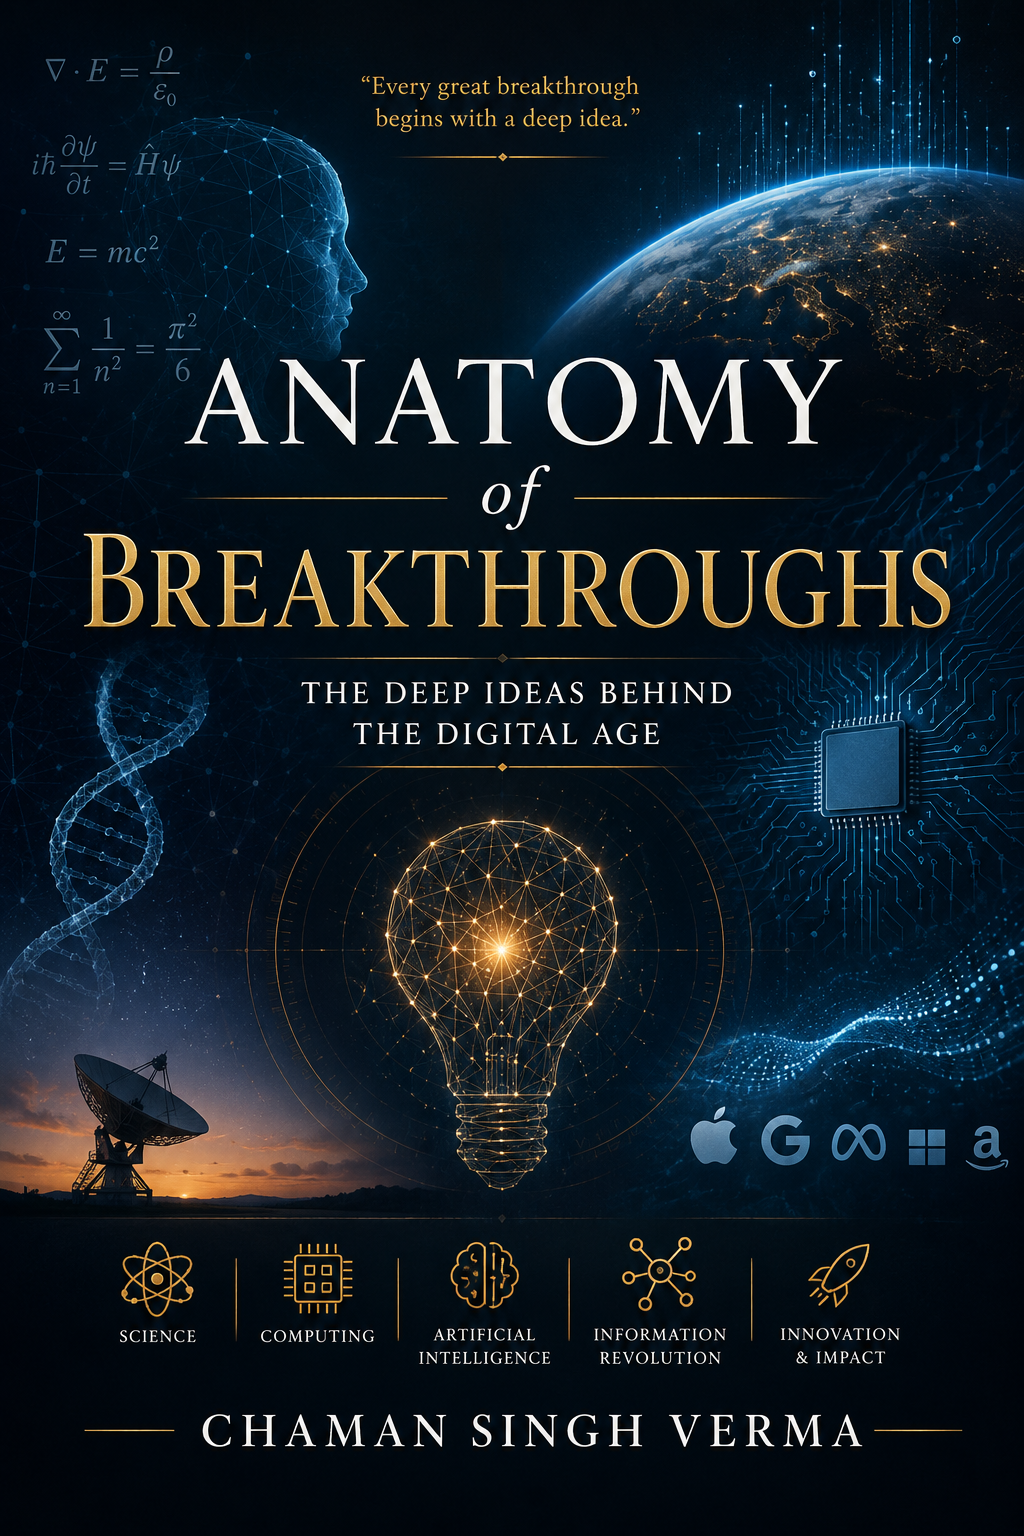
\includegraphics[width=\textwidth,height=\textheight,keepaspectratio]{frontpage.png}

\vfill

\noindent\begin{minipage}{0.85\textwidth}
\small
\textbf{Abstract.}---This monograph presents a systematic study of the foundational ideas that shaped modern computer science, information theory, and computational complexity. Fourteen chapters examine breakthroughs spanning computability (Turing machines, the Church--Turing Thesis), undecidability (the halting problem, Gödel's incompleteness theorems, Rice's Theorem), information theory (Shannon entropy, channel capacity, error-correcting codes), algorithmic information (Kolmogorov complexity, algorithmic randomness), computational complexity (P vs NP, NP-completeness, the PCP theorem), cryptography (public-key systems, zero-knowledge proofs, post-quantum schemes), distributed computing (consensus protocols, the FLP impossibility theorem), and interactive proofs (IP = PSPACE, multi-prover systems). Each chapter develops the relevant mathematics rigorously, situating the results within their historical and conceptual context. The epilogue identifies nine recurring cognitive patterns across these breakthroughs and analyzes their applicability to contemporary research in computer science, artificial intelligence, and related disciplines. The intended audience includes graduate students and researchers in theoretical computer science, mathematics, and the foundations of computation. Prerequisites include discrete mathematics, linear algebra, and probability theory.
\end{minipage}

\end{titlepage}

\maketitle

\tableofcontents

%%%%%%%%%%%%%%%%%%%%%%%%%%%%%%%%%%%%%%%%%%%%%%%%%%%%%%%%%%%%%%
\chapter*{Preface}
\addcontentsline{toc}{chapter}{Preface}

This monograph presents a systematic study of the foundational ideas that shaped modern computer science, information theory, and computational complexity. Fourteen chapters examine breakthroughs spanning computability (Turing machines, the Church--Turing Thesis), undecidability (the halting problem, G{\"o}del's incompleteness theorems, Rice's Theorem), information theory (Shannon entropy, channel capacity, error-correcting codes), algorithmic information (Kolmogorov complexity, algorithmic randomness), computational complexity (P vs. NP, NP-completeness, the PCP theorem), cryptography (public-key systems, zero-knowledge proofs, post-quantum schemes), distributed computing (consensus protocols, the FLP impossibility theorem), and interactive proofs (IP = PSPACE). Each chapter develops the relevant mathematics rigorously, situating the results within their historical and conceptual context. The epilogue identifies nine recurring cognitive patterns across these breakthroughs and analyzes their applicability to contemporary research in computer science, artificial intelligence, and related disciplines.

\section*{Methodology}
\addcontentsline{toc}{section}{Methodology}

Each chapter is organized around a consistent analytical framework:

\begin{enumerate}
\item \textbf{The Question} --- What problem was the community trying to solve?
\item \textbf{Why It Seemed Impossible} --- What conceptual barriers prevented progress?
\item \textbf{Historical Context} --- What was known at the time, and what related ideas were emerging?
\item \textbf{The Mental Leap} --- The creative insight that resolved the impasse.
\item \textbf{The Mathematics} --- A rigorous development of the theory, with formal definitions, theorems, and proofs.
\item \textbf{Consequences} --- What became possible as a result of this breakthrough?
\item \textbf{Philosophical Significance} --- What does this reveal about the nature of knowledge, computation, or reality?
\item \textbf{Modern Legacy} --- Where does this idea appear in contemporary research and applications?
\item \textbf{Summary and Key Takeaways} --- A concise synthesis of the chapter's arguments and results.
\end{enumerate}

This framework is not prescriptive; it is descriptive. The nine sections reflect the structure that emerges when a breakthrough is analyzed retrospectively: the question that motivated it, the barriers that obscured it, the insight that dissolved it, and the consequences that followed.

\section*{Selection Criteria}
\addcontentsline{toc}{section}{Selection Criteria}

Every chapter satisfies \emph{all} of the following criteria:

\begin{enumerate}
\item Introduced an entirely new conceptual framework.
\item Permanently changed computer science, mathematics, or engineering.
\item Influenced adjacent disciplines beyond its immediate domain.
\item Retains significance and generates active research more than a decade after its discovery.
\item Represents a qualitative advance rather than an incremental improvement.
\end{enumerate}

These criteria are deliberately restrictive. Many important ideas in computer science are excluded: they are technically significant but represent refinements of existing frameworks rather than the creation of new ones. The book focuses on discoveries that could not have been anticipated from the state of knowledge that preceded them.

\section*{Scope and Organization}
\addcontentsline{toc}{section}{Scope and Organization}

The chapters are organized into four parts:

\begin{itemize}
\item \textbf{Part I: The Nature of Computation} (Chapters 1--4) --- Establishes the foundations of computability theory.
\item \textbf{Part II: Information} (Chapters 5--7) --- Develops the theory of information and its manipulation.
\item \textbf{Part III: Difficulty and Coordination} (Chapters 8--13) --- Explores computational complexity, cryptography, and distributed consensus.
\item \textbf{Part IV: Epilogue} (Chapter 14) --- Identifies recurring patterns of insight across the preceding chapters.
\end{itemize}

Part I establishes the formal notion of computation and its limits. Part II extends the discussion to information, its measurement, and its protection. Part III examines the nature of computational difficulty, the harnessing of hardness for cryptographic purposes, and the coordination of distributed systems. Part IV synthesizes the preceding material into a taxonomy of cognitive patterns underlying breakthrough discoveries.

\section*{Intended Audience and Background}
\addcontentsline{toc}{section}{Intended Audience and Background}

This monograph is intended for graduate students and researchers in theoretical computer science, mathematics, and related fields. The prerequisites include:

\begin{itemize}
\item \textbf{Discrete mathematics:} Sets, functions, relations, induction, combinatorics.
\item \textbf{Linear algebra:} Vector spaces, matrices, eigenvalues, determinants (primarily Chapters 6 and 12).
\item \textbf{Probability theory:} Random variables, expectation, variance, concentration inequalities (primarily Chapters 8--13).
\item \textbf{Basic programming:} Understanding of algorithmic correctness (helpful for computational exercises).
\end{itemize}

A self-contained review of mathematical prerequisites is provided in the appendix. Each chapter is largely self-contained; however, earlier chapters provide essential background for later ones.

\section*{Notation}
\addcontentsline{toc}{section}{Notation}

Standard notation from computability theory, complexity theory, and information theory is used throughout. Key notation is summarized in the Mathematical Prerequisites appendix. Greek letters denote mathematical objects ($\mathbb{N}$, $\mathbb{Z}$, $\mathbb{Q}$, $\mathbb{R}$, $\mathbb{C}$), capital Roman letters denote complexity classes (P, NP, PSPACE, EXP), and lowercase Roman letters denote specific algorithms or protocols.

\mainmatter

%%%%%%%%%%%%%%%%%%%%%%%%%%%%%%%%%%%%%%%%%%%%%%%%%%%%%%%%%%%%%%
\part{The Nature of Computation}

%%%%%%%%%%%%%%%%%%%%%%%%%%%%%%%%%%%%%%%%%%%%%%%%%%%%%%%%%%%%%%
\include{chapters/01_what_is_computation}
% Chapter 2: The Halting Problem
% Part I: The Nature of Computation

\chapter{The Halting Problem}
\label{ch:halting}

%======================================================================
% SECTION 1: THE QUESTION
%======================================================================
\section{The Question: What Problem Was Humanity Trying to Solve?}
\label{sec:halting:question}

After Turing defined what computation \emph{is}, the immediate next question was: \emph{What can computation do?} Specifically, can a computer program analyze another computer program and predict its behavior?

\begin{question}Can a computer determine whether another computer will ever stop?\end{question}

More formally: Does there exist a program $H$ such that for any program $P$ and input $x$, $H(P, x)$ outputs ``halts'' if $P$ halts on $x$, and ``loops'' if $P$ runs forever on $x$?

\begin{highlightbox}[The Core Question]Is the halting behavior of a program a decidable property? Can we automate the task of debugging infinite loops — the most frustrating and time-consuming aspect of programming?\end{highlightbox}

This wasn't just a practical question about debugging. It was the \emph{Entscheidungsproblem} in disguise. If we could decide halting, we could decide any mathematical statement expressible as ``does this program halt?'' — which, via G\"odel numbering, is essentially all of mathematics.

The Entscheidungsproblem (German for ``decision problem''), posed by David Hilbert in 1928, asked whether there exists an algorithm that can determine the truth or falsity of any given logical statement. Hilbert believed that such an algorithm must exist — after all, mathematicians reason systematically, and that reasoning could presumably be mechanized. The halting problem is a concrete version of this grand question: instead of asking about arbitrary logical statements, we ask about the simplest non-trivial behavior of a program.

This framing transforms an abstract philosophical question into a precise mathematical one. If we cannot decide halting — the simplest possible question about a program's behavior — then we certainly cannot decide arbitrary mathematical truth. The halting problem became the linchpin of undecidability.

%======================================================================
% SECTION 2: WHY IT SEEMED IMPOSSIBLE
%======================================================================
\section{Why It Seemed Impossible}
\label{sec:halting:impossible}

The idea that we \emph{cannot} build a halting detector was deeply counterintuitive. After all:

\begin{enumerate}
\item \textbf{We do it manually:} Programmers trace through code, find infinite loops, prove termination. Why can't we automate this reasoning?

\item \textbf{Programs are finite:} A program is a finite string. Its behavior on a given input is determined. In principle, the answer exists — the program either halts or it doesn't. Why can't we compute it?

\item \textbf{Many special cases are decidable:} Programs without loops always halt. Programs with simple bounded loops halt. Linear arithmetic loops halt. The undecidable cases seem like pathological exceptions.

\item \textbf{The Universal Machine exists:} We can \emph{simulate} any program. If we simulate $P$ on $x$ and it halts, we know it halts. The problem is only when it \emph{doesn't} halt — we'd have to simulate forever to be sure.

\item \textbf{Every problem has an algorithm:} Hilbert's program was rooted in the belief that all mathematical questions are decidable in principle. The prevailing view among mathematicians in the early 20th century was that any well-posed problem has a solution that can be found by mechanical reasoning.
\end{enumerate}

\begin{roadblockbox}[The Intuition Trap]
``Just simulate it for a very long time. If it hasn't halted by then, it probably won't.'' This heuristic fails catastrophically: there are programs that run for $10^{10^{10}}$ steps and then halt. There is no computable bound on halting time. The busy beaver function $\Sigma(n)$ grows faster than any computable function; for $n=5$, $\Sigma(5) = 47,\!176,\!870$, but for $n=6$, the value is already beyond what any existing formal system can prove.

\end{roadblockbox}

\begin{roadblockbox}[Hilbert's Faith]
Hilbert declared in 1930: ``Wir m\"ussen wissen — wir werden wissen'' (We must know — we shall know). This was not naive optimism; it was a deeply held philosophical conviction that the universe of mathematics is completely knowable. G\"odel, Church, and Turing shattered this conviction within six years.

\end{roadblockbox}

The mathematical community expected a positive answer. Hilbert's program \emph{required} it. The discovery that the answer is \textbf{no} — and that the proof is devastatingly simple — was a shock that reverberated through mathematics, logic, and philosophy.

%======================================================================
% SECTION 3: HISTORICAL CONTEXT
%======================================================================
\section{Historical Context: What Was Known at the Time}
\label{sec:halting:context}

\begin{historicalbox}[1936: The Annus Mirabilis of Computability]
In a single year, three independent proofs of undecidability appeared:
\begin{itemize}
\item \textbf{Turing (May 1936):} Halting problem undecidable via diagonalization on Universal TM.
\item \textbf{Church (April 1936):} Entscheidungsproblem undecidable via $\lambda$-calculus (received before Turing's paper).
\item \textbf{Post (1936):} ``Post correspondence problem'' undecidable; tag systems.
\end{itemize}
Turing's proof is the most accessible and directly addresses the ``mechanical procedure'' intuition.

\end{historicalbox}

Key context:

\begin{itemize}
\item \textbf{(\cite{godel1931}) G{"o}del's Incompleteness (1931):} Showed that in any consistent formal system, there are true but unprovable statements. But G\"odel's proof was \emph{non-constructive} — it showed existence without giving a specific undecidable \emph{problem}. The halting problem gave a \emph{concrete, natural} undecidable problem.

\item \textbf{Diagonalization (Cantor 1891):} The technique that proves the reals are uncountable. Turing adapted it to computation: list all programs, construct one that differs from each on its own index.

\item \textbf{Self-Reference Paradoxes:} The Liar Paradox (``This statement is false''), Russell's Paradox (set of all sets not containing themselves). Turing's proof is a computational version of the Liar Paradox.

\item \textbf{Finite Combinatory Processes (Post 1936):} Emil Post independently developed a formulation of computation nearly identical to Turing's. His paper ``Finite Combinatory Processes — Formulation 1'' described what we now call a Post machine. Tragically, Post suffered from bipolar disorder and his work was delayed; he received word of Turing's results before publishing, but his contributions were acknowledged.
\end{itemize}

\begin{connectionbox}[Connection to Chapter 1]
The Universal Turing Machine (Chapter 1) is the \emph{enabler} of the halting problem proof. Without a single machine that can simulate all others, diagonalization across ``all programs'' has no formal meaning. Universality makes the set of all programs a single, well-defined object.

\end{connectionbox}

\subsection*{The Priority Dispute}

Turing's paper was submitted to the \emph{Proceedings of the London Mathematical Society} on May 28, 1936. Church's paper was submitted to the \emph{Journal of Symbolic Logic} in April 1936. Post's paper was submitted in 1936 as well. All three were working independently. The convergence of three different approaches (Turing machines, $\lambda$-calculus, canonical systems) on the same result — undecidability — was powerful evidence that the result was fundamental, not an artifact of any particular formalism.

\subsection*{The Church--Turing Dynamic}

The relationship between Church and Turing was complex. Church was Turing's PhD advisor at Princeton, yet their approaches to the Entscheidungsproblem were completely different. Church used G\"odel's recursive functions and his own lambda calculus to show that there is no algorithm for deciding validity in first-order logic. Turing invented an entirely new formalism — a-mathematical machines (later called Turing machines) — that was concretely mechanical rather than abstractly logical.

When Turing submitted his paper, Church served as a referee. \cite{turing1937}, Church insisted that Turing acknowledge the equivalence of his machines to $\lambda$-definability — a result Turing proved in his 1937 PhD thesis. This equivalence became foundational: it showed that all reasonable formalizations of computation capture the same class of functions, giving birth to the Church--Turing thesis.

Turing's paper was communicated by M. H. A. Newman and published in two parts (1936-37). The term ``Church-Turing thesis'' was coined later by Kleene.

\subsection*{Post's Delayed Publication}

Emil Post is a figure whose work was profoundly affected by bipolar disorder. He independently discovered the undecidability of the halting problem but delayed publication due to his condition. By the time he was ready to publish, Church's and Turing's papers had already appeared. \cite{post1936}, Post's paper ``Finite Combinatory Processes — Formulation 1'' was published in 1936 but added a valuable perspective: the \emph{tag system}, a remarkably simple model of computation that is also universal.

Post later posed what became known as \emph{Post's problem}: Do there exist recursively enumerable sets that are neither decidable nor complete (i.e., of intermediate Turing degree)? This question drove research in computability theory for over a decade until its solution by Friedberg and Muchnik in 1956-57.

\begin{historicalbox}[Key Figures]
\begin{itemize}
\item \textbf{Alan Turing (1912--1954):} British mathematician, logician, cryptanalyst, and computer scientist. Defined the Turing machine, broke the Enigma code at Bletchley Park, and made foundational contributions to artificial intelligence (Turing test), morphogenesis, and early computer design.

\item \textbf{Alonzo Church (1903--1995):} American mathematician and logician. Invented the lambda calculus, proved the undecidability of the Entscheidungsproblem, formulated the Church--Turing thesis. PhD advisor to Turing and many other pioneers.

\item \textbf{Emil Post (1897--1954):} Polish-American mathematician. Made foundational contributions to computability theory, including Post's problem, Post Correspondence Problem, and tag systems. His work was profoundly affected by bipolar disorder.

\item \textbf{Stephen C. Kleene (1909--1994):} American mathematician. Student of Church. Developed the recursion theorem, the arithmetical hierarchy, and the theory of recursive functions. Coined the term ``Church--Turing thesis.''
\end{itemize}

\end{historicalbox}

\subsection*{The G\"odel--Turing Correspondence}

An often-overlooked historical detail is G\"odel's reaction to Turing's work. \cite{godel1931}, In 1931, G{"o}del had shown the existence of undecidable propositions — statements that can neither be proved nor disproved within a given formal system. However, G\"odel's construction was highly artificial; it was unclear whether \emph{natural} mathematical problems might be undecidable.

When Turing's paper arrived, G\"odel immediately recognized its significance. In a 1936 letter to Zermelo, G\"odel called Turing's work ``the most important result in the foundations of mathematics'' since his own incompleteness theorems. Turing had shown that undecidability is not an artifact of logical self-reference but a fundamental feature of any computational system.

G\"odel later expressed reservations about Turing's definition of computation, arguing that Turing's machines might not capture all possible forms of effective calculability. However, over time, G\"odel accepted the Church--Turing thesis as the correct characterization of computability.

\subsection*{The Broader Intellectual Climate}

The 1930s was a remarkable decade for mathematical logic. The Vienna Circle was promoting logical positivism, and Hilbert's program was still the dominant philosophy of mathematics. The year 1936 alone saw not just the work of Church, Turing, and Post, but also Gentzen's consistency proof for arithmetic (using transfinite induction), Rosser's strengthening of G\"odel's incompleteness theorem, and Kleene's development of general recursive functions.

The convergence of so many foundational results in a single year was no coincidence. The Entscheidungsproblem was widely discussed, and the tools for solving it — G\"odel numbering, diagonalization, self-reference — were all in place. The intellectual climate was ripe for a resolution, whether positive or negative.

\subsection*{The Aftermath: Recognition and Tragedy}

Turing's paper was initially met with skepticism. Even G\"odel, who recognized its importance, initially doubted that Turing machines captured all computation. The mathematical establishment was slow to accept that such a fundamental limitation existed.

Turing continued his work at Princeton, completing his PhD under Church in 1938. He then returned to England, where he worked on cryptanalysis at Bletchley Park during World War II. After the war, he worked on the ACE computer design and contributed to early AI research. His death in 1954 (by cyanide poisoning, ruled suicide) cut short one of the most brilliant careers in the history of science.

Church continued his work in logic, supervising 29 PhD students including Turing, Kleene, and many others who shaped the field. He spent most of his career at Princeton, later moving to UCLA.

Post struggled with bipolar disorder throughout his life, eventually dying by electroconvulsive therapy in 1954 — the same year as Turing. His contributions were recognized posthumously, and Post's problem remained open for over a decade after his death.

%======================================================================
% SECTION 4: THE MENTAL LEAP
%======================================================================
\section{The Mental Leap: The Creative Insight That Changed Everything}
\label{sec:halting:leap}

\begin{mentalLeap}[The Insight]Turn the universal machine against itself. If a halting decider $H$ exists, build a machine $D$ that does the \emph{opposite} of what $H$ predicts on its own code. Feed $D$ its own description. Contradiction.\end{mentalLeap}

The leap is not the diagonalization — Cantor did that. The leap is: \emph{programs are data}. A program can take \emph{itself} as input. The universal machine makes ``program-as-data'' possible, and self-application is the dagger.

Turing's proof constructs a \emph{liar machine}:

\begin{enumerate}
\item Assume $H$ exists: $H(\langle P \rangle, x) = \text{``halts''}$ iff $P$ halts on $x$.
\item Define $D(\langle P \rangle)$: Run $H(\langle P \rangle, \langle P \rangle)$. If $H$ says ``halts'', loop forever. If $H$ says ``loops'', halt.
\item Run $D$ on its own description: $D(\langle D \rangle)$.
\item If $D(\langle D \rangle)$ halts, then $H(\langle D \rangle, \langle D \rangle) = \text{``halts''}$, so $D$ loops — contradiction.
\item If $D(\langle D \rangle)$ loops, then $H(\langle D \rangle, \langle D \rangle) = \text{``loops''}$, so $D$ halts — contradiction.
\item Therefore $H$ cannot exist.
\end{enumerate}

\begin{roadblockbox}[Why This Was Hard to See]
Before Turing, ``a program analyzing another program'' was a meta-level activity — something a \emph{human} does. The idea that a program could \emph{be} the input to another program (including itself) required the stored-program concept: code = data. This is the conceptual leap from ``calculating with numbers'' to ``calculating with calculations.''

\end{roadblockbox}

\subsection*{The Diagonalization Pattern}

The halting problem proof follows a template that appears throughout mathematics:

\begin{enumerate}
\item Assume a complete enumeration exists (of programs, reals, theorems, etc.)
\item Construct an object that differs from the $i$-th entry on its own index $i$ (the diagonal)
\item The constructed object cannot be in the enumeration — contradiction
\end{enumerate}

This same pattern proves:
\begin{itemize}
\item Cantor's theorem: $|\mathbb{R}| > |\mathbb{N}|$ (diagonalize on decimal expansions)
\item Russell's paradox: $\{x \mid x \notin x\}$ (diagonalize on set membership)
\item G\"odel's first incompleteness: $G \leftrightarrow \neg\text{Prov}(\ulcorner G \urcorner)$ (diagonalize on provability)
\item Tarski's undefinability of truth (diagonalize on truth predicate)
\item Rice's theorem (diagonalize on semantic properties)
\item Time/space hierarchy theorems (diagonalize on bounded computation)
\end{itemize}

\subsection*{The Deeper Insight: Self-Reference Is Inescapable}

The halting problem proof reveals something significant about any system powerful enough to represent its own processes. Once a system can talk about itself — once programs can be treated as data — paradox becomes inevitable. This is not a bug; it is a feature of the logical universe. The same self-reference that enables a Universal Turing Machine to simulate any program is the self-reference that prevents any program from solving the halting problem.

Lawvere's fixed-point theorem (1969) generalizes this pattern: in any category with sufficient structure, every endomorphism of an object that has a point-surjective map from itself to its function space has a fixed point. The halting problem, G\"odel's theorem, Russell's paradox, and Cantor's theorem are all instances of this same categorical principle.

\begin{roadblockbox}[Self-Application as the Essential Ingredient]
Turing's key innovation was not diagonalization itself — it was the realization that programs can be applied to themselves. The Universal Turing Machine from Chapter 1 computes a function $U(\langle P \rangle, x) = P(x)$. The halting proof uses $U$ with the same program in both positions: $U(\langle P \rangle, \langle P \rangle)$. This self-application is what creates the contradiction. Without it, diagonalization would have no purchase.

\end{roadblockbox}

%======================================================================
% SECTION 5: THE MATHEMATICS
%======================================================================
\section{The Mathematics: Rigorous Development of the Theory}
\label{sec:halting:math}

\subsection{Formal Definitions}
\label{sec:halting:definitions}

\begin{definition}[Halting Problem]
The \emph{halting problem} $\HALT$ is the language:
\[
\HALT = \{ \langle M, w \rangle \mid M \text{ is a TM that halts on input } w \}
\]
The \emph{halting decision problem} asks: Is $\HALT$ decidable (i.e., recursive)?
\end{definition}

\begin{definition}[Decidable Language]
A language $L \subseteq \Sigma^*$ is \emph{decidable} (recursive) if there exists a TM $M$ that halts on all inputs and $L(M) = L$.
\end{definition}

\begin{definition}[Semi-Decidable (Recursively Enumerable)]
A language $L$ is \emph{semi-decidable} (r.e.) if there exists a TM $M$ such that $L(M) = L$ (M halts and accepts on $w \in L$; may loop on $w \notin L$).
\end{definition}

\subsection{The Undecidability Proof}
\label{sec:halting:proof}

\begin{theorem}[Turing 1936: The Halting Problem Is Undecidable]
$\HALT$ is not decidable.
\end{theorem}

\begin{proof}
Assume for contradiction that $\HALT$ is decidable. Then there exists a TM $H$ that halts on all inputs and:
\[
H(\langle M, w \rangle) = 
\begin{cases}
\text{accept} & \text{if } M \text{ halts on } w \\
\text{reject} & \text{if } M \text{ loops on } w
\end{cases}
\]

Construct a new TM $D$:
\begin{enumerate}
\item On input $\langle M \rangle$ (description of a TM):
\item Run $H(\langle M, \langle M \rangle \rangle)$.
\item If $H$ accepts, \emph{loop forever}.
\item If $H$ rejects, \emph{halt}.
\end{enumerate}

Now consider $D$ on input $\langle D \rangle$:
\begin{itemize}
\item If $D(\langle D \rangle)$ halts, then $H(\langle D, \langle D \rangle \rangle)$ accepts, so $D$ loops — contradiction.
\item If $D(\langle D \rangle)$ loops, then $H(\langle D, \langle D \rangle \rangle)$ rejects, so $D$ halts — contradiction.
\end{itemize}

Therefore $H$ cannot exist. $\HALT$ is undecidable.
\end{proof}

\subsection*{A More Detailed Construction}

The proof above is the standard textbook version. For completeness, we present a more explicit Turing machine construction. Let $U$ be the Universal Turing Machine from Chapter 1. We construct $H$ as a two-stage TM:

\begin{enumerate}
\item $H$ reads input $\langle M, w \rangle$ and writes the transition table of $M$ onto its working tape.
\item $H$ simulates $M$ step by step, using $U$'s simulation technique.
\item If the simulation reaches a halt state, $H$ enters an accept state.
\item If the simulation enters a configuration it has seen before (a loop), $H$ enters a reject state.
\end{enumerate}

The critical point is step 4: detecting a loop is itself undecidable. But for the proof, we assume $H$ can do this — that is the assumption we will contradict.

The diagonal machine $D$ is then constructed as:
\begin{enumerate}
\item $D$ reads $\langle M \rangle$.
\item $D$ computes $\langle M, \langle M \rangle \rangle$ — pairing $M$ with its own description.
\item $D$ feeds this pair to $H$.
\item If $H$ accepts, $D$ enters an infinite loop (a simple cycle that never halts).
\item If $H$ rejects, $D$ halts immediately.
\end{enumerate}

The self-application $D(\langle D \rangle)$ creates the paradox. Note that $D$ does not need to ``understand'' the program it is checking — it simply follows the instructions described above.

\subsection{\texorpdfstring{$\HALT$}{HALT} Is Semi-Decidable}
\label{sec:halting:semidecidable}

\begin{theorem}
$\HALT$ is recursively enumerable (semi-decidable).
\end{theorem}

\begin{proof}
The Universal TM $U$ accepts $\HALT$: on input $\langle M, w \rangle$, simulate $M$ on $w$. If $M$ halts, $U$ accepts. If $M$ loops, $U$ loops. Thus $L(U) = \HALT$.
\end{proof}

\subsection{The Complement Is Not Semi-Decidable}
\label{sec:halting:complement}

\begin{theorem}
$\overline{\HALT}$ is \emph{not} recursively enumerable.
\end{theorem}

\begin{proof}
If both $\HALT$ and $\overline{\HALT}$ were r.e., then $\HALT$ would be decidable (run both semi-deciders in parallel; one must accept). But $\HALT$ is undecidable.
\end{proof}

\begin{corollary}
There exist languages that are not recursively enumerable.
\end{corollary}

\begin{theorem}[The Halting Problem Is Not Co-r.e.]
$\overline{\HALT}$ is not semi-decidable; equivalently, $\HALT$ is not co-r.e.
\end{theorem}

\begin{proof}
If $\overline{\HALT}$ were r.e., then $\HALT$ would be both r.e. and co-r.e., which would make it decidable. This contradicts Turing's theorem.
\end{proof}

\subsection{Many-One Reductions: Proving Other Problems Undecidable}
\label{sec:halting:reductions}

\begin{definition}[Many-One Reduction]
$A \le_m B$ if there exists a computable function $f$ such that $x \in A \iff f(x) \in B$.
\end{definition}

\begin{proposition}
If $A \le_m B$ and $B$ is decidable, then $A$ is decidable. Contrapositive: If $A$ is undecidable and $A \le_m B$, then $B$ is undecidable.
\end{proposition}

\begin{example}[The Blank Tape Halting Problem]
$\HALT_0 = \{ \langle M \rangle \mid M \text{ halts on empty input } \epsilon \}$.
Reduce $\HALT$ to $\HALT_0$: Given $\langle M, w \rangle$, construct $M_w$ that ignores its input, writes $w$ on the tape, then simulates $M$. $M$ halts on $w \iff M_w$ halts on $\epsilon$.
\end{example}

\begin{example}[The Totality Problem]
$\TOT = \{ \langle M \rangle \mid M \text{ halts on all inputs} \}$.
$\TOT$ is $\Pi^0_2$-complete (see arithmetical hierarchy below). Undecidable by reduction from $\HALT$.
\end{example}

\begin{example}[The Equivalence Problem]
$\EQ = \{ \langle M_1, M_2 \rangle \mid L(M_1) = L(M_2) \}$.
Undecidable by reduction from $\HALT$.
\end{example}

\begin{example}[The Emptiness Problem]
$\EMPTY = \{ \langle M \rangle \mid L(M) = \emptyset \}$.
Given $\langle M, w \rangle$, construct $M'$ that on any input $x$: first simulates $M$ on $w$; if $M$ halts, then simulate a universal machine on $x$ and accept if $x$ is accepted. If $M$ does not halt on $w$, $M'$ never halts. Then $L(M') = \emptyset$ iff $M$ does not halt on $w$. Hence $\overline{\HALT} \le_m \EMPTY$, so $\EMPTY$ is undecidable.
\end{example}

\begin{example}[The Regularity Problem]
$\REG = \{ \langle M \rangle \mid L(M) \text{ is regular} \}$.
Given $\langle M, w \rangle$, construct $M'$ that recognizes a non-regular language (e.g., $\{0^n 1^n \mid n \ge 0\}$) if $M$ halts on $w$, and the empty language otherwise. Then $M'$ is regular iff $M$ does not halt on $w$, reducing $\overline{\HALT} \le_m \REG$.
\end{example}

\begin{example}[The Context-Free Problem]
$\CFL = \{ \langle M \rangle \mid L(M) \text{ is context-free} \}$.
Similar construction: use a context-sensitive language (e.g., $\{0^n 1^n 2^n\}$) in place of the non-regular language. Shows that even determining whether a TM's language is context-free is undecidable.
\end{example}

\subsection*{Worked Example: Reduction from $\HALT$ to $\HALT_0$}

Consider how we reduce $\HALT$ to the blank-tape halting problem $\HALT_0$. Given $\langle M, w \rangle$ we construct $M_w$ as follows:

Construction of $M_w$: On input $x$:
\begin{enumerate}
\item Erase $x$ and write $w$ onto the tape.
\item Return the head to the start of $w$.
\item Simulate $M$ on $w$.
\end{enumerate}

Now:
\begin{itemize}
\item If $M$ halts on $w$, then $M_w$ halts on the empty tape (since it writes $w$ and then halts after $M$). So $\langle M_w \rangle \in \HALT_0$.
\item If $M$ does not halt on $w$, then $M_w$ loops on the empty tape (since it gets stuck simulating $M$). So $\langle M_w \rangle \notin \HALT_0$.
\end{itemize}

Thus $\langle M, w \rangle \in \HALT \iff f(\langle M, w \rangle) = \langle M_w \rangle \in \HALT_0$, and $f$ is clearly computable (we can print the code of $M_w$ given the code of $M$ and the string $w$). This reduction is surpisingly simple — the key idea is to ignore the input and hardcode the simulation.

\subsection*{Worked Example: Reduction in Detail}

\[
M \text{ halts on } w \iff M' \text{ halts on all inputs}
\]

Construction of $M'$: On input $x$:
\begin{enumerate}
\item Ignore $x$ and simulate $M$ on $w$.
\item If $M$ halts on $w$, then simulate a universal machine on $\langle \text{count}, x \rangle$ where $\text{count}$ is a TM that counts from $0$ to $|x|$ and halts.
\end{enumerate}

Now:
\begin{itemize}
\item If $M$ halts on $w$, then $M'$ always executes step 2, which halts for any $x$ (counting is total). So $M' \in \TOT$.
\item If $M$ does not halt on $w$, then $M'$ loops at step 1 for every input $x$. So $M' \notin \TOT$.
\end{itemize}

Thus $\HALT \le_m \TOT$, proving $\TOT$ is undecidable. This construction illustrates the general technique: embed the halting simulation as the first step, and use the branching to encode the answer.

\subsection*{Worked Example: Reduction from $\HALT$ to $\EQ$}

The equivalence problem $\EQ$ asks whether two Turing machines accept the same language. To show it is undecidable, reduce $\HALT$ to $\EQ$:

Given $\langle M, w \rangle$, construct two machines $M_1$ and $M_2$:
\begin{itemize}
\item $M_1$: On any input $x$, simulate $M$ on $w$. If $M$ halts, accept $x$. Otherwise, loop.
\item $M_2$: On any input $x$, accept $x$ immediately.
\end{itemize}

Now:
\begin{itemize}
\item If $M$ halts on $w$, then $M_1$ accepts all inputs (like $M_2$), so $\langle M_1, M_2 \rangle \in \EQ$.
\item If $M$ does not halt on $w$, then $M_1$ accepts no inputs (it loops on all), while $M_2$ accepts all inputs, so $\langle M_1, M_2 \rangle \notin \EQ$.
\end{itemize}

Thus $\HALT \le_m \EQ$, proving $\EQ$ is undecidable. This pattern — comparing a conditional machine with a fixed machine — is a standard trick for reductions to equivalence problems.

\subsection*{Worked Example: The Acceptance Problem}

The acceptance problem $A_{\TM} = \{ \langle M, w \rangle \mid M \text{ accepts } w \}$ is closely related to $\HALT$. In fact, they are many-one equivalent:

\begin{enumerate}
\item $A_{\TM} \le_m \HALT$: Given $\langle M, w \rangle$, modify $M$ to $M'$ that enters an infinite loop whenever $M$ would reject. Then $M$ accepts $w \iff M'$ halts on $w$.
\item $\HALT \le_m A_{\TM}$: Given $\langle M, w \rangle$, modify $M$ to $M'$ that accepts whenever $M$ would halt. Then $M$ halts on $w \iff M'$ accepts $w$.
\end{enumerate}

This equivalence shows that the difficulty of halting and the difficulty of accepting are the same — neither is harder than the other.

\subsection{Turing Reductions and Degrees of Unsolvability}
\label{sec:halting:turing}

Many-one reductions ($\le_m$) are not the only way to compare difficulty.

\begin{definition}[Turing Reduction]
$A \le_T B$ if there exists an oracle TM that decides $A$ given oracle access to $B$.
\end{definition}

While a many-one reduction is a single computable transformation from instances of $A$ to instances of $B$, a Turing reduction allows multiple queries to the oracle for $B$, possibly with adaptive queries where the choice of the next query depends on the answer to the previous one. This makes Turing reductions strictly more powerful than many-one reductions.

\begin{example}[Turing vs. Many-One]
Consider $\HALT$ and $\overline{\HALT}$. Clearly $\overline{\HALT} \le_T \HALT$: to decide if $\langle M, w \rangle \in \overline{\HALT}$, just query the $\HALT$ oracle and negate the answer. However, $\overline{\HALT} \not\le_m \HALT$ in general, because a many-one reduction would require a single total computable function mapping the complement into the original set, which would imply $\HALT$ is both r.e. and co-r.e. and hence decidable.
\end{example}

\begin{example}[Truth-Table vs. Turing Reductions]
Some problems require more than one query. Consider the problem of determining whether two machines $M_1$, $M_2$ have the same halting behavior on input $w$. A truth-table reduction (a Turing reduction where all queries are made in parallel) would ask two questions to $\HALT$ and then compute the answer. This is less powerful than a full Turing reduction where later queries depend on earlier answers.
\end{example}

\begin{definition}[Turing Degree]
The \emph{Turing degree} of $A$ is the equivalence class $\{ B \mid A \equiv_T B \}$ under mutual Turing reducibility.
\end{definition}

\subsection*{The Jump Operator and Turing Degrees}

\begin{definition}[Turing Jump]
The \emph{Turing jump} $A'$ of a set $A$ is the halting problem relativized to oracle $A$:
\[
A' = \{ \langle M \rangle \mid M^A \text{ halts on } \langle M \rangle \}
\]
where $M^A$ denotes a TM with oracle access to $A$.
\end{definition}

The jump operator provides a way to ascend through ever-harder problems. Starting from the empty set $\emptyset$, we define $\emptyset^{(0)} = \emptyset$, $\emptyset^{(1)} = \emptyset' = \HALT$, $\emptyset^{(2)} = \HALT'$, and so on. The $n$-th jump $\emptyset^{(n)}$ is the halting problem relativized to $\emptyset^{(n-1)}$.

\begin{theorem}[Post 1944]
$\HALT$ is the \emph{complete} r.e. degree: for any r.e. set $A$, $A \le_T \HALT$. Moreover, $\HALT$ has strictly higher degree than any decidable set.
\end{theorem}

\begin{theorem}[Kleene-Post 1954]
There exist r.e. degrees strictly between $\mathbf{0}$ (decidable) and $\mathbf{0}'$ (degree of $\HALT$).
\end{theorem}

\subsection*{The Recursion Theorem (Kleene 1938)}

One of the most powerful results in computability theory is Kleene's recursion theorem, which formalizes the intuition that programs can refer to their own code.

\begin{theorem}[Kleene's Recursion Theorem]
For any computable function $f: \N \to \N$, there exists an integer $e$ (called a \emph{fixed point}) such that $\varphi_e = \varphi_{f(e)}$, where $\varphi_i$ denotes the partial computable function computed by the $i$-th Turing machine.
\end{theorem}

\begin{proof}
Define a computable function $d(u)$ that, given input $u$, produces the index of a TM that does the following: on input $x$, simulate $\varphi_u(u)$ to obtain an index $v$, then simulate $\varphi_v(x)$. By the s-m-n theorem, $d$ is total computable.

Since $f$ is computable, $f \circ d$ is also computable. Let $u_0$ be an index for $f \circ d$. Set $e = d(u_0)$. Then:

\[
\varphi_e(x) = \varphi_{d(u_0)}(x) = \varphi_{\varphi_{u_0}(u_0)}(x) = \varphi_{(f \circ d)(u_0)}(x) = \varphi_{f(d(u_0))}(x) = \varphi_{f(e)}(x)
\]

Thus $\varphi_e = \varphi_{f(e)}$, as desired.
\end{proof}

The recursion theorem has many applications:

\begin{itemize}
\item \textbf{Self-reproducing programs (quines):} Choose $f$ to be a constant function that always outputs a fixed index $i$. The fixed point $e$ satisfies $\varphi_e = \varphi_i$. Thus there exists a program that does the same thing as the program indexed by $i$ — but more interestingly, the theorem guarantees the existence of programs that can refer to their own source code.

\item \textbf{The fixed-point formulation of incompleteness:} G\"odel's first incompleteness theorem can be proved using the recursion theorem: there exists a sentence that asserts its own unprovability.

\item \textbf{Recursive definitions:} The existence of a program satisfying $\varphi_e(x) = f(e, x)$ follows from the recursion theorem, enabling self-referential definitions in recursion theory.

\item \textbf{Coinductive definitions:} For infinite computations, the recursion theorem guarantees the existence of fixed points for computable transformations on infinite objects.
\end{itemize}

\subsection*{The S-m-n Theorem and Parameterization}

A key technical tool that underpins many reductions is the S-m-n theorem (also called the parameterization theorem):

\begin{theorem}[Kleene's S-m-n Theorem]
For each $m, n \ge 1$, there exists a computable function $S^m_n$ such that for all indices $e$ and all tuples $\vec{a}$ (length $m$), $\vec{b}$ (length $n$):
\[
\varphi_{S^m_n(e, \vec{a})}(\vec{b}) = \varphi_e(\vec{a}, \vec{b})
\]
\end{theorem}

In words: we can ``hardcode'' the first $m$ arguments of a program into a new program that takes only the remaining $n$ arguments. This is the formal justification for the construction $M_w$ we used in the reduction from $\HALT$ to $\HALT_0$. Given a TM $M$ and a string $w$, we needed to build a new TM $M_w$ that ignores its input and simulates $M$ on $w$. The S-m-n theorem guarantees that this transformation is computable.

The S-m-n theorem is also essential for proving the recursion theorem and for many constructions in computability theory. In programming terms, it is the theoretical basis for partial application and currying.

\begin{example}[Using S-m-n for Reductions]
To reduce $\HALT$ to $\HALT_0$: given $\langle M, w \rangle$, we want $\langle M_w \rangle$ such that $M_w$ halts on $\epsilon$ iff $M$ halts on $w$. The S-m-n theorem gives us a computable function $f$ such that:
\[
f(\langle M, w \rangle) = \langle M_w \rangle
\]
where $M_w$ ignores its input, writes $w$, and simulates $M$. The existence of $f$ as a computable function is guaranteed by S-m-n.
\end{example}

\subsection*{Post's Problem and Priority Arguments}

Post's problem, formulated by Emil Post in 1944, asks: Does there exist a recursively enumerable set $A$ that is neither decidable nor complete (i.e., neither $\emptyset \le_T A$ nor $\HALT \le_T A$)? In other words, is the structure of r.e. Turing degrees one-dimensional (just decidable and complete) or is there a richer structure?

\begin{historicalbox}[Post's Problem]
``Post's problem'' was the most famous open problem in computability theory for over a decade. Post himself made numerous unsuccessful attempts to solve it, developing partial results and intermediate concepts. The problem was finally solved independently by Richard Friedberg (a 20-year-old undergraduate at Harvard) and Albert Muchnik (a graduate student in Moscow) in 1956--57. Their solution introduced the \emph{priority method}, which became the central technique in modern computability theory.

\end{historicalbox}

The \emph{priority method} (or \emph{finite injury} method) works as follows:

\begin{enumerate}
\item We want to build two r.e. sets $A$ and $B$ such that neither is Turing-computable from the other.
\item We enumerate requirements: for each TM $M$, we must ensure $M$ does not decide $A$ (or $B$), and that $B$ is not reducible to $A$ (or vice versa).
\item Requirements are assigned \emph{priorities} (a ranking). When two requirements conflict, the higher-priority one wins.
\item At each stage of the construction, we attempt to satisfy the highest-priority unsatisfied requirement. We may need to ``injure'' previously satisfied lower-priority requirements by changing the sets. But since each requirement can be injured only finitely many times (by higher-priority requirements), all requirements are eventually satisfied.
\end{enumerate}

This ``finite injury'' method was revolutionary because it introduced the idea of dynamic, priority-driven constructions where earlier decisions might need to be undone. The method has been generalized to infinite injury, priority trees, and other sophisticated techniques.

\subsection*{The Friedberg--Muchnik Theorem}

\begin{theorem}[Friedberg 1957, Muchnik 1956]
There exist r.e. Turing degrees strictly between $\mathbf{0}$ and $\mathbf{0}'$. Equivalently, there exists an r.e. set $A$ that is neither decidable nor Turing-equivalent to $\HALT$.
\end{theorem}

\begin{proof}[Sketch]
We construct an r.e. set $A$ that satisfies two families of requirements:
\begin{itemize}
\item $R_{2e}$: $A \neq \{e\}$ (ensuring $A$ is not decidable), where $\{e\}$ is the $e$-th decidable set.
\item $R_{2e+1}$: $\HALT \not\le_T A$ via the $e$-th Turing reduction (ensuring $A$ is not complete).
\end{itemize}

We assign priorities: $R_0 > R_1 > R_2 > \cdots$. At stage $s$, we work on the highest-priority requirement $R_i$ that is not yet satisfied. To satisfy $R_{2e}$, we find an $x$ such that $x \in A \iff x \notin \{e\}$. To satisfy $R_{2e+1}$, we find an $x$ in $\HALT$ such that the $e$-th oracle machine with oracle $A$ gives the wrong answer about $x$.

When a lower-priority requirement is injured by a higher-priority one, it must restart its work. The finite injury lemma guarantees that each requirement is injured only finitely often, so the construction converges to a set $A$ satisfying all requirements.
\end{proof}

The Friedberg--Muchnik theorem was a landmark result that opened up the study of the structure of the r.e. degrees. It showed that the Turing degrees of r.e. sets form a dense partial order with infinitely many incomparable elements.

The \emph{arithmetical hierarchy} classifies degrees by the logical complexity of definitions:

\subsection{The Arithmetical Hierarchy}
\label{sec:halting:hierarchy}

\begin{definition}[Arithmetical Hierarchy]
\begin{itemize}
\item $\Sigma^0_0 = \Pi^0_0 = \Delta^0_0$ = computable (recursive) relations
\item $\Sigma^0_{n+1}$ = relations definable by $\exists x_1 \forall x_2 \dots Q x_{n+1} \, R(x_1, \dots, x_{n+1})$ where $R \in \Pi^0_n$
\item $\Pi^0_{n+1}$ = relations definable by $\forall x_1 \exists x_2 \dots Q x_{n+1} \, R(x_1, \dots, x_{n+1})$ where $R \in \Sigma^0_n$
\item $\Delta^0_n = \Sigma^0_n \cap \Pi^0_n$
\end{itemize}
\end{definition}

\begin{theorem}[Hierarchy Placement]
\begin{itemize}
\item $\HALT \in \Sigma^0_1$ (r.e.) and is $\Sigma^0_1$-complete
\item $\overline{\HALT} \in \Pi^0_1$ (co-r.e.) and is $\Pi^0_1$-complete
\item $\TOT = \{ \langle M \rangle \mid M \text{ halts on all inputs} \} \in \Pi^0_2$ and is $\Pi^0_2$-complete
\item $\mathsf{FIN} = \{ \langle M \rangle \mid M \text{ halts on finitely many inputs} \} \in \Sigma^0_2$ and is $\Sigma^0_2$-complete
\item $\mathsf{COF} = \{ \langle M \rangle \mid M \text{ halts on cofinitely many inputs} \} \in \Sigma^0_3$ and is $\Sigma^0_3$-complete
\item $\mathsf{REC} = \{ \langle M \rangle \mid L(M) \text{ is decidable} \} \in \Sigma^0_3$ and is $\Sigma^0_3$-complete
\end{itemize}
\end{theorem}

\begin{proof}[Sketch for $\TOT \in \Pi^0_2$]
$M \in \TOT \iff \forall x \exists t \, [M \text{ halts on } x \text{ in } t \text{ steps}]$.
The predicate ``$M$ halts on $x$ in $t$ steps'' is computable (simulate $t$ steps).
So $\TOT$ has form $\forall \exists$ computable $\to \Pi^0_2$.
\end{proof}

\subsection*{Detailed Classification}

The arithmetical hierarchy can be understood intuitively:

\begin{itemize}
\item $\Sigma^0_1$ (r.e.): Properties that can be verified by a finite search. $\HALT$ is $\Sigma^0_1$ because we can search for a halting computation.
\item $\Pi^0_1$ (co-r.e.): Properties that can be refuted by a finite search. $\overline{\HALT}$ is $\Pi^0_1$ because we can search for a contradiction to the claim that a program halts (though this search may never end).
\item $\Sigma^0_2$: Properties of the form ``there exists an $x$ such that for all $y$, a computable predicate holds.'' Example: ``$M$ halts on finitely many inputs'' means there is a bound $b$ such that for all inputs $y > b$, $M$ loops on $y$.
\item $\Pi^0_2$: Properties of the form ``for all $x$, there exists a $y$ such that a computable predicate holds.'' Example: ``$M$ halts on all inputs'' means for every input $x$, there is a computation time $t$ after which $M$ halts.
\item Higher levels continue this alternation of quantifiers, with each alternation adding expressive power.
\end{itemize}

The hierarchy is strict: $\Sigma^0_n \subsetneq \Sigma^0_{n+1}$, $\Pi^0_n \subsetneq \Pi^0_{n+1}$. This means there are genuinely harder problems at each level, and the classification is not arbitrary but reflects the inherent logical complexity.

\begin{theorem}[Post's Theorem]
A set is $\Sigma^0_{n+1}$ iff it is r.e. in $\emptyset^{(n)}$ (the $n$-th jump of the empty set).
\end{theorem}

\subsection*{The Jump Operator in Detail}

The \emph{Turing jump} $A'$ of a set $A$ is the halting problem relativized to oracle $A$:
\[
A' = \{ \langle M \rangle \mid M^A \text{ halts on } \langle M \rangle \}
\]
Then $\emptyset^{(n)}$ is the $n$-th iterate of the jump.

The jump operator creates an infinite hierarchy of unsolvability:
\[
\emptyset <_T \emptyset' <_T \emptyset'' <_T \emptyset''' <_T \cdots
\]

Each jump is strictly harder than the previous one. The arithmetical hierarchy corresponds exactly to this jump hierarchy:
\[
\Sigma^0_{n+1} = \{ A \mid A \text{ is r.e. in } \emptyset^{(n)} \}
\]

This means that the jump operator provides a bridge between the logical complexity of a definition (how many quantifier alternations it has) and the computational difficulty of deciding membership (how many halting-problem oracles are needed).

\subsection{The Structure of r.e. Degrees}

The Turing degrees of r.e. sets form a rich partial order. Key results:

\begin{itemize}
\item \textbf{Existence of minimal pairs:} There exist non-computable r.e. sets $A$ and $B$ such that any set computable from both $A$ and $B$ is computable. (Lachlan 1966, Yates 1966)
\item \textbf{Density:} Between any two r.e. degrees $\mathbf{a} < \mathbf{b}$, there exists an r.e. degree $\mathbf{c}$ with $\mathbf{a} < \mathbf{c} < \mathbf{b}$. (Sacks 1964)
\item \textbf{Incomparability:} There exist r.e. degrees $\mathbf{a}$ and $\mathbf{b}$ such that neither $\mathbf{a} \le_T \mathbf{b}$ nor $\mathbf{b} \le_T \mathbf{a}$. (Friedberg--Muchnik 1956/57)
\item \textbf{Non-existence of minimal r.e. degree:} There is no r.e. degree strictly above $\mathbf{0}$ that is below all other non-zero r.e. degrees.
\end{itemize}

\subsection*{Priority Arguments in the Modern Context}

The priority method introduced by Friedberg and Muchnik has become the foundational technique of modern computability theory. There are now many variants:

\begin{itemize}
\item \textbf{Finite injury priority:} Each requirement is injured only finitely often. Used for Friedberg--Muchnik, Sacks density theorem.
\item \textbf{Infinite injury priority:} Requirements may be injured infinitely often, but the injury is controlled in some way. Used for more complex degree constructions.
\item \textbf{Tree priority:} Requirements are organized on a tree structure, with branching based on oracle answers. Used for the ``plus-cupping'' theorem and other advanced results.
\item \textbf{``Priority on steroids'':} Modern techniques allow the construction of degrees with extremely specific structural properties.
\end{itemize}

\subsection*{Halting and Incompleteness: The Deep Connection}

One of the most significant consequences of the halting problem is its connection to G\"odel's incompleteness theorems. The two results are, in a precise sense, the same theorem viewed through different lenses.

G\"odel's first incompleteness theorem states: for any consistent formal system $F$ capable of expressing arithmetic, there exists a sentence $G_F$ such that $F$ neither proves nor refutes $G_F$. The halting problem gives a constructive version: there exists a specific Turing machine $M$ and input $w$ such that $M$ does not halt on $w$, but $F$ cannot prove this fact.

In fact, we can construct such a machine explicitly: let $M_{\text{G\"odel}}$ be a machine that searches for a proof of $0 = 1$ in $F$. If such a proof is found, it halts. If $F$ is consistent, $M_{\text{G\"odel}}$ never halts, but $F$ cannot prove that $M_{\text{G\"odel}}$ never halts (because if it could, it would prove its own consistency, violating G\"odel's second incompleteness theorem).

This connection shows that the halting problem and G\"odel's theorem are two sides of the same coin. G\"odel showed that there are true but unprovable statements; Turing showed that among those statements are concrete claims about program behavior. The arithmetical hierarchy further refines this: at each level $\Sigma^0_n$, we encounter statements that are true but whose truth requires $n$ levels of unbounded quantification to express.

\begin{connectionbox}[Connections to Later Chapters]
\begin{itemize}
\item Chapter 4 (Rice's Theorem): Generalizes the halting problem's undecidability to all non-trivial semantic properties of programs.
\item Chapter 7 (Kolmogorov Complexity): The uncomputability of $K(x)$ follows from a reduction to $\HALT$.
\item Chapter 8 (Complexity): The arithmetical hierarchy is the logical precursor to the polynomial hierarchy $\PH$, which separates problems by quantifier alternation in bounded time.
\end{itemize}

\end{connectionbox}

%======================================================================
% SECTION 6: CONSEQUENCES
%======================================================================
\section{Consequences: What Became Possible}
\label{sec:halting:consequences}

The halting problem's undecidability is not a negative result — it is a \emph{structural} result that shapes all of computer science:

\begin{enumerate}
\item \textbf{No Perfect Debugger:} There can be no tool that infallibly detects infinite loops. Every static analyzer must either miss some bugs (false negatives) or flag correct code (false positives) — or not terminate. This tradeoff is not a design limitation; it is a mathematical inevitability.

\item \textbf{Compiler Optimizations Are Heuristics:} Determining if two programs are equivalent, if a loop terminates, if a variable is used — all undecidable. Compilers use conservative approximations. For example, dead code elimination cannot always determine whether code is reachable; it errs on the side of keeping potentially dead code.

\item \textbf{Type Systems Are Conservative:} A type system that accepts all safe programs and rejects all unsafe ones would solve the halting problem. Real type systems reject some safe programs. This is why Rust's borrow checker rejects some valid programs, and why Java's type system cannot verify certain correctness properties.

\item \textbf{Program Verification Is Inherently Hard:} Proving arbitrary properties of programs (Rice's Theorem, Chapter 4) is undecidable. Verification tools require human guidance (invariants, annotations). This is not a limitation of current tools — it is a fundamental constraint on what can be automated.

\item \textbf{The Foundation of Complexity:} The halting problem separates \emph{computable} from \emph{uncomputable}. Complexity theory (Chapter 8) separates \emph{efficiently computable} from \emph{intractable}. The former is a hard boundary; the latter is a practical one.

\item \textbf{G\"odel's Incompleteness, Made Constructive:} The halting problem gives an \emph{explicit} undecidable problem. G\"odel's theorem says ``some statement is unprovable''; Turing says ``here is a specific program whose halting behavior is unprovable.''

\item \textbf{Rice's Theorem (Chapter 4):} The halting problem is the seed from which Rice's theorem grows — it generalizes undecidability to \emph{all} non-trivial semantic properties.

\item \textbf{The Arithmetical Hierarchy:} The jump operator and degrees of unsolvability create a rich structure above the computable sets, with $\HALT$ as the first step.

\item \textbf{Abstract Interpretation (Cousot \& Cousot 1977):} Rather than trying to solve undecidable problems exactly, abstract interpretation computes safe approximations. By defining an abstract semantics that over-approximates all possible behaviors, static analyzers can prove the absence of certain bugs, at the cost of false positives. This tradeoff is the direct consequence of the halting problem.

\item \textbf{Model Checking:} Finite-state model checking is decidable because the state space is finite. The halting problem tells us why infinite-state systems require abstraction, bisimulation, or other approximation techniques.

\item \textbf{The Limits of AI:} No AI system can, in general, determine whether another AI system will enter an infinite loop. This has implications for AI safety, formal verification of learned systems, and the theoretical limits of automated reasoning.

\item \textbf{Symbolic Execution and Concolic Testing:} Tools like KLEE and SAGE use symbolic execution to explore program paths. The halting problem ensures they cannot cover all paths; they must use heuristics to prioritize which paths to explore. This is why symbolic execution tools can find deep bugs but cannot provide complete coverage guarantees.

\item \textbf{Operating System Scheduling:} The halting problem underlies the impossibility of scheduling algorithms that can always distinguish between a process in an infinite loop and a process that will eventually produce output. Time-sharing systems use preemptive scheduling precisely because they cannot trust programs to voluntarily yield.

\item \textbf{Malware Detection:} Determining whether an arbitrary program is malicious is a form of the halting problem. If we could decide maliciousness, we could decide halting (by constructing a program that behaves maliciously iff it halts). This is why antivirus software relies on signatures, heuristics, and behavioral analysis rather than perfect detection.

\item \textbf{Database Query Optimization:} Determining whether two SQL queries are equivalent is undecidable in general, as is determining whether a query terminates. Query optimizers use equivalence-preserving transformations, which are sound but incomplete.

\item \textbf{Protocol Verification:} Verifying that a communication protocol terminates (no infinite waits, no deadlocks) is undecidable for general infinite-state protocols. Tools like SPIN and TLA+ use finite-state abstractions or theorem proving.
\end{enumerate}

\begin{roadblockbox}[The Undecidability Tradeoff]
Every static analysis tool faces the same fundamental tradeoff: soundness (no false negatives) is incompatible with completeness (no false positives) for any non-trivial property. This is not a flaw in the tool — it is the halting problem in action. The art of static analysis is choosing the right approximation to maximize useful answers while accepting the inevitable gaps.

\end{roadblockbox}

%======================================================================
% SECTION 7: PHILOSOPHICAL SIGNIFICANCE
%======================================================================
\section{Philosophical Significance: What It Taught Us About Knowledge, Computation, or Reality}
\label{sec:halting:philosophy}

\begin{enumerate}
\item \textbf{Knowledge Has Hard Limits:} Not just ``we don't know yet'' — \emph{provably cannot know}. The halting problem is not a puzzle waiting for a clever solution. It is a boundary of the knowable. This is a fundamentally different kind of limitation from those encountered in everyday science (where new theories overturn old ones). It is a limitation intrinsic to the very nature of computation.

\item \textbf{Self-Reference Creates Paradox:} The proof is a computational Liar Paradox. Any system powerful enough to represent its own programs (self-reference) inherits the paradox. This applies to formal systems (G\"odel), truth predicates (Tarski), and computation (Turing). The common thread is that self-reference introduces a diagonalization that cannot be contained.

\item \textbf{Prediction Requires Simulation:} To know what a program does, one must essentially run it. There is no ``shortcut'' to the future of a computation. This is \emph{computational irreducibility} (Wolfram 2002) — the only way to know the outcome is to perform the computation. This principle has significant implications for physics (can the universe simulate itself faster than it runs?), biology (can a brain predict its own future states?), and economics (can a market predict its own behavior?).

\item \textbf{The Map Is Not the Territory, But the Program Is the Machine:} In physics, a simulation approximates reality. In computation, the simulation \emph{is} the reality. The universal machine doesn't model computation — it \emph{is} computation. This collapse of the map-territory distinction is unique to computation and explains why the halting problem is so fundamental.

\item \textbf{Uncertainty Is Intrinsic, Not Epistemic:} We don't fail to solve the halting problem because we lack information. We fail because the answer \emph{does not exist} as a computable function. This is ontological, not epistemological. It is not a limitation of our ingenuity; it is a limitation of the mathematical structure of computation itself.

\item \textbf{The Hierarchy of Ignorance:} The arithmetical hierarchy shows that undecidability comes in degrees. $\HALT$ is just the first step. There are problems strictly harder than $\HALT$, and harder still, ad infinitum. Each jump represents a new level of uncomputability. This hierarchy is not merely a mathematical curiosity — it reflects the fact that some truths require more powerful reasoning methods than others.

\item \textbf{The Mind--Body Problem:} The halting problem has been invoked in discussions of consciousness and the mind-body problem. If human mathematicians can solve instances of the halting problem that cannot be solved by any fixed formal system (as some argue via G\"odel's theorem), then human reasoning is not computable. This argument, most famously advanced by Roger Penrose, is controversial but illustrates the halting problem's reach beyond computer science.

\item \textbf{Free Will and Determinism:} The halting problem provides a precise mathematical model of a deterministic system whose future states cannot be predicted by any algorithm within the same system. This suggests that determinism does not imply predictability — a distinction with implications for debates about free will.

\item \textbf{Computational Irreducibility in Physics:} Stephen Wolfram's Principle of Computational Equivalence suggests that many physical systems are computationally universal, and hence their behavior is computationally irreducible. The halting problem implies that predicting the long-term behavior of such systems is fundamentally impossible without simulating them step by step.

\item \textbf{The Nature of Mathematical Proof:} The halting problem tells us that there is no general algorithm for proving theorems. Each theorem requires its own insight. This is not a limitation of current mathematics — it is a fundamental fact about the relationship between proof and truth. G\"odel showed that some truths are unprovable; Turing showed that even the truth of halting statements is unprovable in general.

\item \textbf{The Limits of Reductionism:} The halting problem demonstrates that the behavior of a deterministic system cannot always be predicted by analyzing its components. A Turing machine's behavior is completely determined by its transition table and input, yet predicting whether it halts is beyond any algorithmic analysis. This is a precise mathematical instance of emergence: the whole is not reducible to its parts in any computational sense.

\item \textbf{Algorithmic Information Theory:} The halting problem connects to Kolmogorov complexity (Chapter 7) through Chaitin's $\Omega$, the halting probability. $\Omega$ is a well-defined real number whose digits encode the solutions to all halting problems. Yet $\Omega$ is uncomputable and its digits are algorithmically random — they cannot be compressed into any finite theory. This unifies three deep ideas: undecidability, randomness, and incompleteness.

\item \textbf{The Parable of the Perfect Tool:} The halting problem teaches us that there is no perfect tool — no algorithm that solves all instances of a non-trivial problem. Every tool makes tradeoffs. The most sophisticated verification systems (separation logic, dependent types, interactive theorem provers) all require human guidance. Accepting this limitation is not defeat; it is the beginning of wisdom in software engineering.
\end{enumerate}

%======================================================================
% SECTION 8: MODERN LEGACY
%======================================================================
\section{Modern Legacy: Where This Idea Appears Today}
\label{sec:halting:legacy}

\begin{itemize}
\item \textbf{Static Analysis / Abstract Interpretation:} All sound static analyzers (Astree, Infer, CodeQL) must over-approximate. They answer ``definitely halts,'' ``maybe halts,'' ``definitely loops'' — the middle category is unavoidable. Modern tools like Infer (Facebook/Meta) and Astree (Airbus) handle millions of lines of code using clever approximations that are guaranteed to be sound.

\item \textbf{Termination Checkers:} Tools like AProVE, T2, Julia's termination analysis prove termination for restricted classes (size-change termination, polynomial interpretations). They succeed on real code but cannot be complete. The state of the art can handle most practical programs while remaining sound.

\item \textbf{Smart Contract Verification:} Ethereum's gas limit exists \emph{because} halting is undecidable. Without a step bound, a contract could run forever, freezing the blockchain. Gas meters are an engineering solution to an undecidable problem: instead of determining whether a program halts, we bound the resources it can consume.

\item \textbf{Model Checking:} Finite-state model checking (SPIN, NuSMV) is decidable because the state space is finite. But infinite-state systems (programs with unbounded integers, recursion) hit the halting barrier. Tools like SLAM and BLAST use predicate abstraction to model infinite-state systems with finite approximations.

\item \textbf{AI Safety / Interpretability:} Can we build an AI that proves it won't enter an infinite loop? The halting problem says: not in general. This constrains formal verification of AI behavior. However, for specific AI architectures (e.g., transformer networks with finite context), we can sometimes prove termination.

\item \textbf{Busy Beaver and the Limits of Mathematics:} $\Sigma(n)$ (maximum halting steps for $n$-state TM) grows faster than any computable function. Determining $\Sigma(5)$ required proving that a specific 5-state TM runs for 47,176,870 steps — the boundary of what mathematics can currently decide. $\Sigma(6)$ is unknown and likely beyond current mathematics.

\item \textbf{Chaitin's $\Omega$ (Chapter 7):} The halting probability $\Omega = \sum_{p: U(p)\downarrow} 2^{-|p|}$ is a real number that encodes the halting problem. Its bits are algorithmically random and unprovable in any fixed formal system. $\Omega$ is a concrete example of a number that is well-defined but whose digits cannot be computed.

\item \textbf{Post's Correspondence Problem (PCP):} A simple undecidable problem about matching strings. Used to prove undecidability of many problems in formal languages, compiler optimization, and database theory. PCP is particularly useful for reductions because its simplicity makes it adaptable to many domains.

\item \textbf{Hilbert's 10th Problem:} The undecidability of Diophantine equations (Matiyasevich 1970) builds on the halting problem. Hilbert asked for an algorithm to determine whether any polynomial equation with integer coefficients has integer solutions. Matiyasevich showed this is equivalent to the halting problem, providing another natural undecidable problem outside logic.

\item \textbf{Word Problem for Groups:} Determining whether a given word in a group presentation equals the identity is undecidable (Novikov 1955, Boone 1959). This connects the halting problem to abstract algebra, showing that undecidability appears in group theory as well.

\item \textbf{Program Obfuscation:} The halting problem underlies the impossibility of perfect obfuscation. If we could perfectly obfuscate programs, we could solve the halting problem by comparing obfuscated behaviors. This leads to the concept of indistinguishability obfuscation (iO), which is a best-possible approximation.

\item \textbf{The Lambda Calculus:} Church's lambda calculus was the first formalism in which undecidability was proved. The $\beta$-reduction problem (does a lambda term have a normal form?) is the halting problem for the lambda calculus. This connects directly to functional programming languages like Haskell and OCaml.

\item \textbf{Interactive Theorem Proving:} Systems like Coq, Isabelle, and Lean require users to guide proofs precisely because the halting problem makes fully automated theorem proving impossible. These tools succeed by combining automation with human insight, embodying the ``good enough'' philosophy that the halting problem necessitates.

\item \textbf{Type Inference in Advanced Type Systems:} Undecidable type inference in languages like Haskell (with GADTs, type families, and dependent types) is a direct consequence of the halting problem. GHC's type checker uses various heuristics and conservative approximations, rejecting some valid programs to ensure termination of type checking.

\item \textbf{Concurrency and Deadlock Detection:} Determining whether a concurrent program will deadlock is undecidable in general. Tools like Rust's Send/Sync traits and Go's race detector use static and dynamic approximations that are sound but incomplete. The halting problem explains why there can be no perfect deadlock detector.

\item \textbf{Bioinformatics and Protein Folding:} The halting problem appears unexpectedly in bioinformatics: determining whether a cellular automaton or a gene regulatory network reaches a stable state is often undecidable. This constrains what can be proved about biological systems and guides the development of simulation-based approaches.

\item \textbf{Computational Neuroscience:} The question of whether a neural network will converge during training is a form of the halting problem. This explains why training algorithms use stopping criteria (gradient thresholds, patience) rather than convergence guarantees.

\item \textbf{Programming Language Design:} Modern programming languages increasingly acknowledge the halting problem. Rust's borrow checker accepts a conservative approximation of memory safety. TypeScript's type system is deliberately not Turing-complete to ensure decidability. Even so, TypeScript's type-level computation can simulate a Turing machine, leading to undecidable type checking in pathological cases.
\end{itemize}

\begin{connectionbox}[Connections]
\begin{itemize}
\item Chapter 1 (Computation): Universal TM enables the proof.
\item Chapter 3 (G\"odel): Halting problem is the computational face of incompleteness.
\item Chapter 4 (Rice's Theorem): Generalizes halting to \emph{all} semantic properties.
\item Chapter 7 (Kolmogorov): Chaitin's $\Omega$ encodes $\HALT$; $K(x)$ is uncomputable (reduction from halting).
\item Chapter 8 (Complexity): Halting is the ``decidable vs. undecidable'' boundary; P vs NP is the ``efficient vs. intractable'' boundary.
\end{itemize}

\end{connectionbox}

%======================================================================
% SECTION 9: LESSONS FOR FUTURE SCIENTISTS
%======================================================================
\section{Summary}
\label{sec:halting:summary}

This chapter established the undecidability of the halting problem, proving that no algorithm can determine whether an arbitrary Turing machine halts on a given input. The proof employed Cantor's diagonalization technique, adapted to the computational setting via self-reference: a hypothetical halting decider is fed its own description, yielding a contradiction analogous to the liar paradox. The chapter formalized the notions of recursively enumerable (r.e.) and recursive (decidable) languages, establishing that the halting problem is r.e. but not recursive. Rice's Theorem was presented as a generalization of the halting problem, showing that every non-trivial semantic property of Turing machines is undecidable. The chapter also discussed the arithmetical hierarchy, locating the halting problem at $\Sigma^0_1$-completeness and the totality problem $\text{TOT}$ at $\Pi^0_2$-completeness. Various reductions from HALT were demonstrated, including to the blank-tape halting problem, the emptiness problem, and the Post Correspondence Problem. The recursion theorem (Kleene 1938) was introduced as a powerful self-reference tool, showing that any computable transformation of a program's description can be realized by a program that has access to its own description. The chapter concluded with a discussion of computational irreducibility (Wolfram 2002) and the Busy Beaver function, which grows faster than any computable function and provides a concrete witness to the limits of formal systems.

\section*{Key Takeaways}
\begin{itemize}
\item The halting problem is undecidable: no Turing machine can decide whether an arbitrary Turing machine halts on a given input, proven by diagonalization and self-reference.
\item The halting problem is recursively enumerable but not recursive; it is $\Sigma^0_1$-complete in the arithmetical hierarchy.
\item Rice's Theorem generalizes the undecidability of the halting problem to all non-trivial semantic properties of Turing machines.
\item The recursion theorem provides a formal mechanism for self-reference in computation, underpinning quines, self-replicating programs, and fixed-point combinators.
\item Open problems include the precise classification of problems in the arithmetical hierarchy, the construction of intermediate recursively enumerable degrees (Post's problem, resolved by Friedberg--Muchnik), and the determination of Busy Beaver values for small state counts.
\end{itemize}

%======================================================================
% EXERCISES
%======================================================================
% EXERCISES
%======================================================================
\section{Exercises}
\label{sec:halting:exercises}

\begin{exercise}[Basic]
Prove that the language $\{ \langle M \rangle \mid M \text{ halts on at least one input} \}$ is undecidable by reducing from $\HALT$.
\end{exercise}

\begin{exercise}[Basic]
Show that $\HALT$ is not decidable by reducing from the \emph{acceptance problem} $A_{\TM} = \{ \langle M, w \rangle \mid M \text{ accepts } w \}$.
\end{exercise}

\begin{exercise}[Basic]
Prove that the blank tape halting problem $\HALT_0$ is undecidable.
\end{exercise}

\begin{exercise}[Basic]
Prove that the language $\{ \langle M \rangle \mid M \text{ halts on exactly three inputs} \}$ is undecidable.
\end{exercise}

\begin{exercise}[Basic]
Show that the complement of the halting problem, $\overline{\HALT}$, is not semi-decidable.
\end{exercise}

\begin{exercise}[Intermediate]
A \emph{total computable function} is a function $f: \N \to \N$ computed by a TM that halts on all inputs. Prove that the set of indices of total computable functions is not recursively enumerable. (Hint: diagonalize against all partial computable functions.)
\end{exercise}

\begin{exercise}[Intermediate]
Prove that $\TOT = \{ \langle M \rangle \mid M \text{ halts on all inputs} \}$ is $\Pi^0_2$-complete.
\end{exercise}

\begin{exercise}[Intermediate]
Show that the \emph{index set} for the class of finite languages, $\{ \langle M \rangle \mid L(M) \text{ is finite} \}$, is $\Sigma^0_2$-complete.
\end{exercise}

\begin{exercise}[Intermediate]
Prove that the \emph{recursion theorem} (Kleene 1938) follows from the diagonalization used in the halting problem proof: For any computable $f$, there exists $e$ such that $\varphi_e = \varphi_{f(e)}$.
\end{exercise}

\begin{exercise}[Intermediate]
Let $\INF = \{ \langle M \rangle \mid L(M) \text{ is infinite} \}$. Show that $\INF$ is $\Pi^0_2$-complete. (Hint: reduce $\TOT$ to $\INF$.)
\end{exercise}

\begin{exercise}[Intermediate]
Prove that $\EMPTY = \{ \langle M \rangle \mid L(M) = \emptyset \}$ is not semi-decidable. Show that $\overline{\EMPTY}$ is semi-decidable.
\end{exercise}

\begin{exercise}[Intermediate]
Define a reduction from $\HALT$ to the language $\{ \langle M \rangle \mid M \text{ halts on at most 42 inputs} \}$.
\end{exercise}

\begin{exercise}[Challenge]
Research the \emph{arithmetical hierarchy}: $\Sigma^0_n$, $\Pi^0_n$, $\Delta^0_n$. Where does $\HALT$ sit? Where does $\TOT = \{ \langle M \rangle \mid M \text{ halts on all inputs} \}$ sit? Prove $\TOT$ is $\Pi^0_2$-complete.
\end{exercise}

\begin{exercise}[Challenge]
Research \emph{Priority Arguments} (Friedberg-Muchnik 1956/57). How do they construct r.e. sets of intermediate Turing degree? What is the ``finite injury'' method?
\end{exercise}

\begin{exercise}[Challenge]
Prove \emph{Rice's Theorem} (Chapter 4) directly from the undecidability of $\HALT$. Show that any non-trivial semantic property is undecidable by constructing a reduction from $\HALT$.
\end{exercise}

\begin{exercise}[Challenge]
Prove that the Post Correspondence Problem is undecidable by reduction from $\HALT$. Show at least two concrete PCP instances — one solvable and one unsolvable — alongside the reduction.
\end{exercise}

\begin{exercise}[Challenge]
Show that the problem of determining whether a Diophantine equation has an integer solution (Hilbert's 10th Problem) can be reduced from the halting problem. Explain the key idea of Matiyasevich's theorem.
\end{exercise}

\begin{exercise}[Computational]
Implement a reduction from the halting problem for 2-counter Minsky machines to the halting problem for Turing machines. Verify that the 2-counter machine for the Collatz function ($n \to n/2$ if even, $3n+1$ if odd) halts on all inputs $< 10^6$ (open problem for all inputs!).
\end{exercise}

\begin{exercise}[Computational]
Implement a Universal Turing Machine simulator. Use it to run the 5-state Busy Beaver candidate and verify it runs for 47,176,870 steps.
\end{exercise}

\begin{exercise}[Computational]
Write a program that takes a Python function as input and attempts to prove it terminates using size-change termination. Test it on various recursive functions.
\end{exercise}

\begin{exercise}[Computational]
Implement a simple abstract interpreter that detects non-termination for a toy programming language with bounded loops. Run it on programs that implement the Collatz function, the Ackermann function, and a simple infinite loop. Which ones can your analyzer handle, and why?
\end{exercise}

\begin{exercise}[Computational]
Implement a quine (a program that prints its own source code) in your favorite programming language. Explain how the recursion theorem guarantees its existence.
\end{exercise}

%======================================================================
% TIMELINE
%======================================================================
\section{Timeline}
\label{sec:halting:timeline}
\addcontentsline{toc}{section}{Timeline}

\begin{tabularx}{\linewidth}{|l|X|}
\hline
\textbf{Year} & \textbf{Event} \\ \hline
1891 & Cantor's diagonal argument; uncountability of $\R$ \\ \hline
1901 & Russell's Paradox \\ \hline
1928 & Hilbert poses the Entscheidungsproblem \\ \hline
1931 & G\"odel's Incompleteness Theorems \\ \hline
1936 (Apr) & Church: $\lambda$-calculus; Entscheidungsproblem undecidable \\ \hline
1936 (May) & Turing: ``On Computable Numbers''; TM, Universal TM, Halting Problem \\ \hline
1936 & Post: Tag systems, Post Correspondence Problem \\ \hline
1937 & Turing proves TM $\equiv$ $\lambda$-calculus (PhD under Church) \\ \hline
1938 & Kleene's Recursion Theorem \\ \hline
1943 & McCulloch-Pitts neural networks (finite automata) \\ \hline
1944 & Post: Degrees of unsolvability, Post's problem \\ \hline
1945 & Von Neumann's EDVAC report; stored-program architecture \\ \hline
1954 & Turing dies; the field mourns \\ \hline
1955 & Novikov: Word problem for groups undecidable \\ \hline
1956 & Friedberg-Muchnik: Solution to Post's problem (intermediate r.e. degrees) \\ \hline
1959 & Boone: Word problem for groups undecidable (independent) \\ \hline
1962 & Tarski: Undefinability of truth \\ \hline
1965 & Hartmanis-Stearns: Complexity classes; halting problem is ``just'' the first level \\ \hline
1970 & Matiyasevich: Hilbert's 10th Problem undecidable (Diophantine equations) \\ \hline
1977 & Cousot \& Cousot: Abstract Interpretation — sound approximation of undecidable properties \\ \hline
1984 & Cousot \& Cousot: Formal definition of abstract interpretation \\ \hline
2002 & Wolfram: Computational irreducibility; Principle of Computational Equivalence \\ \hline
2019 & Busy Beaver $\Sigma(5)$ resolved: 47,176,870 steps \\ \hline
2024 & AI verification tools incorporate undecidability-aware techniques \\ \hline
\end{tabularx}

%======================================================================
% CITATIONS
%======================================================================
\section{Citations}
\label{sec:halting:citations}

\begin{enumerate}
  \item \cite{turing1936}
  \item \cite{church1936}
  \item \cite{post1936}
  \item \cite{godel1931}
  \item \cite{davis2000}
  \item \cite{rogers1967}
  \item \cite{soare1987}
  \item \cite{sipser2012}
  \item \cite{aaronson2020}
  \item \cite{wolfram2002}
  \item \cite{hodges1983}
  \item \cite{kleene1936}
  \item \cite{cousot1977}
  \item \cite{myhill1955}
\end{enumerate}

%======================================================================
% INDEX ENTRIES
%======================================================================
\index{halting problem}
\index{undecidability}
\index{diagonalization}
\index{self-reference}
\index{Turing, Alan}
\index{Universal Turing Machine}
\index{recursively enumerable}
\index{semi-decidable}
\index{Rice's Theorem}
\index{computational irreducibility}
\index{Busy Beaver}
\index{arithmetical hierarchy}
\index{Turing jump}
\index{Turing degrees}
\index{Post's problem}
\index{many-one reduction}
\index{Turing reduction}
\index{Post Correspondence Problem}
\index{priority method}
\index{Friedberg-Muchnik theorem}
\index{recursion theorem}
\index{Kleene, Stephen C.}
\index{Church, Alonzo}
\index{abstract interpretation}
\index{model checking}
\index{Entscheidungsproblem}
\index{Hilbert, David}
\index{Church--Turing thesis}

\include{chapters/03_godel_incompleteness}
% Chapter 4: Rice's Theorem
% Part I: The Nature of Computation

\chapter{Rice's Theorem}
\label{ch:rice}

%======================================================================
% SECTION 1: THE QUESTION
%======================================================================
\section{The Question: What Problem Was Humanity Trying to Solve?}
\label{sec:rice:question}

The halting problem (Chapter 2) asks: can we decide if a \emph{specific} program halts on a \emph{specific} input? But programmers care about \emph{properties of programs} --- not just halting. Does this program ever divide by zero? Does it leak memory? Does it compute the correct function? Does it have a buffer overflow? Does it ever access an array out of bounds? Is it susceptible to a race condition? Does it respect a security policy?

Each of these questions asks whether a program satisfies a \emph{property} --- a predicate over all possible executions. A property is \emph{decidable} if there is an algorithm that, given the program source code, can answer yes or no for every program. The surprising discovery of recursion theory is that for virtually any property that depends on what the program \emph{does} (as opposed to how it \emph{looks}), no such algorithm exists.

Formally, we can think of each Turing machine $M$ as having an index $\langle M \rangle$ (its G\"odel number) and computing a partial function $\varphi_{\langle M \rangle}$. A \emph{semantic} property of programs is then a set $\mathcal{P}$ of partial computable functions. The decision problem for $\mathcal{P}$ is: given an index $e$, is $\varphi_e \in \mathcal{P}$? Rice's Theorem answers this question for virtually all interesting $\mathcal{P}$.

Each of these is a question about what a program \emph{does} --- its \emph{semantics} --- not about its syntactic structure. Before Rice's Theorem, the research community confronted a troubling pattern: every interesting semantic question about programs seemed to be undecidable, but the proofs were all different. Was there a \emph{unified} explanation?

\begin{question}
Why are almost all semantic questions about programs undecidable?
\end{question}

More formally: Let $\mathcal{P}$ be a non-trivial property of the function computed by a Turing machine (i.e., a property of the \emph{language} recognized or the \emph{function} computed). Is the set $\{ \langle M \rangle \mid L(M) \text{ has property } \mathcal{P} \}$ decidable?

Rice's Theorem (1953) answers: \textbf{No} --- for \emph{any} non-trivial semantic property.

\begin{highlightbox}[The Core Question]
If the halting problem is undecidable, is that an isolated phenomenon? Or is undecidability the \emph{rule} for reasoning about what programs \emph{do} (as opposed to how they look)?

\end{highlightbox}

\begin{roadblockbox}[The Programmer's Lament]
A working programmer might ask: ``Surely I can \emph{check} whether my program will crash on a given input? one runs it!'' But running it on \emph{one} input does not tell you about \emph{all} inputs. And running it on all inputs would take forever. The question is: can we inspect the code and \emph{decide}, once and for all, whether a property holds for every possible execution? Rice's Theorem says: not if the property is semantic and non-trivial.

\end{roadblockbox}

The theorem draws a sharp line through the space of all possible questions about programs. On one side lie syntactic questions --- ``does this program have more than 100 lines?'' --- which are trivially decidable. On the other side lie semantic questions --- ``does this program compute a prime number?'' --- which are uniformly undecidable. The boundary is not between easy and hard semantic questions; it is between semantic and syntactic questions \emph{tout court}.

\begin{connectionbox}[Connection to Software Engineering]
Every software engineer encounters Rice's Theorem in practice, even if they do not know its name. When a code review asks ``does this function handle all edge cases?'' or ``can this input cause a crash?'' --- these are semantic questions. The theorem tells us that no tool can answer them automatically for arbitrary programs. This is why code review, testing, and formal verification by human experts remain essential: they bring \emph{understanding} to bear where algorithms must fail.

\end{connectionbox}

%======================================================================
% SECTION 2: WHY IT SEEMED IMPOSSIBLE
%======================================================================
\section{Why It Seemed Impossible}
\label{sec:rice:impossible}

Before Rice, the landscape of undecidability was fragmented. Each new undecidability result required a bespoke reduction:

\begin{enumerate}
\item \textbf{The Halting Problem:} Undecidable (Turing 1936).
\item \textbf{The Blank Tape Halting Problem:} Undecidable --- does $M$ halt starting from a blank tape?
\item \textbf{The Totality Problem:} Does $M$ halt on \emph{all} inputs? Undecidable.
\item \textbf{The Equivalence Problem:} Do $M_1$ and $M_2$ compute the same function? Undecidable.
\item \textbf{The Emptiness Problem:} Does $M$ accept any input? Undecidable.
\item \textbf{The Finiteness Problem:} Does $M$ accept a finite language? Undecidable.
\item \textbf{The Regularity Problem:} Does $M$ accept a regular language? Undecidable.
\item \textbf{The Context-Freeness Problem:} Does $M$ accept a context-free language? Undecidable.
\end{enumerate}

Each required its own reduction proof, its own clever encoding, its own diagonalization. It seemed like undecidability was a property of \emph{specific} problems --- some semantic properties might be decidable, others not. There was no \emph{unifying principle}.

\begin{roadblockbox}[The Intuition Trap]
``Surely \emph{some} semantic properties are decidable. For example: `Does this program accept the empty string?' --- just run it on $\epsilon$! If it accepts, yes. If it rejects or loops\ldots oh. We're back to halting.''

The trap: any property that depends on the program's \emph{behavior} on \emph{infinite} inputs inherits the halting problem. But proving this \emph{generally} seemed to require a new proof for each property. Researchers in the 1940s and early 1950s were caught in a pattern of proving each undecidability result individually, without seeing the forest for the trees.

\end{roadblockbox}

\begin{roadblockbox}[The Hidden Assumption]
Another intuition trap: ``What about syntactic semantic properties? For example: `Does this program have exactly 5 states and accept the empty string?' That mixes syntax and semantics --- surely we can decide it?'' The catch: the syntactic part (``5 states'') is decidable, but the semantic part (``accepts the empty string'') is not. The conjunction inherits undecidability from the semantic conjunct. Mixing syntax with semantics does not make the semantic part go away.

\end{roadblockbox}

Experts expected a case-by-case classification: some semantic properties decidable, some not. Rice showed this expectation was wrong --- the boundary is not between properties, but between \emph{trivial} and \emph{non-trivial}. The only decidable semantic properties are those that hold for \emph{every} program or \emph{no} program. Everything else is undecidable.

The prevailing view before Rice was shaped by several prominent near-misses. Post's Correspondence Problem (1944) was a specific undecidable problem about string rewriting, but its proof gave no general template. The word problem for groups (Novikov 1955, Boone 1954) showed undecidability in algebra, but again with a problem-specific proof. Rice's great insight was to see past these individual results to the unifying principle.

To appreciate the difficulty of Rice's insight, consider the state of knowledge in the late 1940s. Researchers had a growing list of undecidable problems but no framework for classifying them. The concept of a \emph{semantic property} had not been formalized. The notion of \emph{index sets} --- sets of G\"odel numbers of programs --- was implicit in G\"odel's work but had not been applied to program properties. The idea that one could prove a theorem about \emph{all} semantic properties at once required seeing programs as data (the insight of the universal Turing machine) and recognizing that the halting problem could be \emph{reduced} to any non-trivial semantic property. This insight was analogous to Cantor's diagonalization: Cantor showed that \emph{any} infinite set has a larger power set; Rice showed that \emph{any} non-trivial semantic property is undecidable.

A skeptic in 1950 might have argued: ``But surely there are semantic properties that are decidable --- for instance, whether a program accepts an input of length exactly 42? We can just run it on all strings of length 42!'' The flaw, of course, is that running a program on all $256^{42}$ possible strings would not terminate if the program loops on any of them. The skeptic's mistake is assuming that ``running the program'' is the same as ``deciding the property.'' Rice's Theorem shows that this assumption is equivalent to solving the halting problem.

\begin{connectionbox}[The P vs.\ NP Connection]
Rice's Theorem also applies to complexity-theoretic properties. Deciding whether a program runs in polynomial time is a semantic property --- it depends on the resource usage of the computation, not the code. Rice tells us this is undecidable. This means that if $\mathsf{P} \neq \mathsf{NP}$, we cannot even \emph{algorithmically verify} that a program solves an $\mathsf{NP}$-complete problem in polynomial time, unless we accept the limitations that Rice imposes. This is one reason why the $\mathsf{P} \neq \mathsf{NP}$ question is so deep: proving that no polynomial-time algorithm exists for a problem is not just hard; it is embedded in a context where even \emph{recognizing} such algorithms is undecidable.

\end{connectionbox}

%======================================================================
% SECTION 3: HISTORICAL CONTEXT
%======================================================================
\section{Historical Context: What Was Known at the Time}
\label{sec:rice:context}

\begin{historicalbox}[Henry Gordon Rice (1920--2003)]
Henry Gordon Rice was born in 1920 in New York. He served in the United States Army during World War II, working on cryptographic problems --- an experience that likely sharpened his interest in the limits of mechanical computation. After the war, he pursued a PhD at Syracuse University under the supervision of J. C. E. Dekker, a leading figure in recursion theory who had made foundational contributions to the theory of creative sets and myriads (a generalization of the concept of ``almost all'' for sets of natural numbers).

Rice's 1951 dissertation, ``Recursive and Recursively Enumerable Sets,'' contained the theorem that would bear his name. \cite{rice1953}. It was published in 1953 in the \emph{Transactions of the American Mathematical Society} under the title ``Classes of Recursively Enumerable Sets and Their Decision Problems.'' After a brief period at the National Security Agency (NSA) during the early Cold War, Rice joined the faculty at Cornell University, where he spent the remainder of his career teaching logic and the foundations of mathematics.

Rice was a quiet, meticulous scholar. He did not seek fame; his theorem emerged from a careful study of the structure of index sets and the classification of recursively enumerable languages. He died in 2003, having witnessed his theorem become a cornerstone of computability theory and program analysis.

\end{historicalbox}

Rice's Theorem was not immediately recognized as the sweeping result it is. The 1950s were a time of rapid development in recursion theory, and many results were being discovered simultaneously. Post's problem --- whether there exist non-recursive, non-complete r.e. Turing degrees --- was solved independently by Friedberg and Muchnik in 1956 using the priority method, which dominated recursion theory for the next two decades. Rice's classification of index sets was initially seen as a helpful classification tool for organizing r.e. sets, but not as the foundational result about program analysis that we recognize today.

\begin{historicalbox}[The Reception of Rice's Theorem]
When Rice's Theorem first appeared, it was received as an elegant piece of recursion theory but not as a revolution. Logicians like Kleene and Post appreciated the classification of index sets, but the theorem's implications for computing practice were not immediately visible. The computing landscape of 1953 was dominated by punch-card machines, assembly language, and nascent compiler technology (Fortran would not appear until 1957). The idea that programs could have undecidable semantic properties was abstract and distant.

It was only in the 1970s, as programming languages matured (ALGOL, Pascal, C), that the theorem's practical bite became clear. Compiler writers trying to optimize code, researchers building program verifiers, and engineers developing testing methodologies all found themselves bumping against Rice's wall. By the 1980s, the theorem was recognized as one of the most practically relevant results in computability theory --- a rare case of a deep mathematical theorem with direct engineering consequences.

\end{historicalbox} Post's problem (whether there exist recursively enumerable sets of intermediate Turing degree) dominated the attention of recursion theorists. Rice's classification of index sets was initially seen as a technical lemma about the structure of r.e. sets rather than a foundational result about program analysis. It took the rise of programming languages, compiler construction, and static analysis in the 1960s and 1970s for the broader significance of Rice's Theorem to become apparent.

The theorem gained prominence through Rogers' influential 1967 textbook \emph{Theory of Recursive Functions and Effective Computability}, which presented Rice's result as one of the central theorems of recursion theory. Rogers showed how index sets could be classified using the arithmetical hierarchy, and how Rice's Theorem fit into the broader program of understanding the degrees of unsolvability. By the 1970s, Rice's Theorem was a standard part of every computability theory curriculum.

Timeline of undecidability results leading to Rice:

\begin{itemize}
\item \textbf{1931:} G\"odel --- Incompleteness Theorems: any consistent formal system containing arithmetic cannot prove its own consistency. This was the first hint that mechanical reasoning has limits.
\item \textbf{1936:} Church --- The Entscheidungsproblem (decision problem for first-order logic) is undecidable. Church used $\lambda$-calculus; Turing used his machines.
\item \textbf{1936:} Turing --- Halting problem undecidable. The first machine-specific undecidability result.
\item \textbf{1938:} Turing --- The oracle machine concept, introducing relative computability and the beginnings of the Turing jump hierarchy.
\item \textbf{1944:} Post --- Post Correspondence Problem undecidable. A purely combinatorial undecidable problem, far removed from computation.
\item \textbf{1950:} Rice's PhD thesis --- ``Recursive and Recursively Enumerable Sets.''
\item \textbf{1951:} Kleene --- The recursion theorem and the arithmetical hierarchy begin to take shape.
\item \textbf{1953:} Rice's Theorem published in the \emph{Transactions of the AMS}.
\item \textbf{1954:} Boone --- Word problem for groups undecidable (independent proof).
\item \textbf{1955:} Myhill --- Creative sets, Rice's Theorem for creative sets, Myhill isomorphism theorem.
\item \textbf{1956:} Myhill-Shepherdson --- Rice-Shapiro Theorem characterizing r.e. index sets.
\item \textbf{1960s:} Rogers --- \emph{Theory of Recursive Functions and Effective Computability} (standard reference that codified Rice's Theorem and its variants).
\end{itemize}

\begin{connectionbox}[Connection to Chapter 2]
Rice's Theorem \emph{generalizes} the halting problem. The halting problem is the special case where $\mathcal{P} = \{ f \mid f(x) \text{ is defined} \}$ for a fixed input $x$. Rice shows this is not a special case at all --- it's the \emph{generic} case. Every non-trivial semantic property is at least as hard as the halting problem.

\end{connectionbox}

\begin{connectionbox}[Connection to G\"odel]
Rice's Theorem is sometimes called ``G\"odel's Theorem for programmers.'' G\"odel showed that any sufficiently powerful formal system cannot decide all arithmetic truths. Rice showed that any sufficiently powerful programming language cannot decide all semantic properties of its own programs. Both are limitative theorems: they draw boundaries around what formal methods can achieve.

\end{connectionbox}

\begin{historicalbox}[The Syracuse School of Recursion Theory]
Syracuse University in the late 1940s and early 1950s was a vibrant center for recursion theory. J. C. E. Dekker, a student of Emil Post at CCNY, had moved to Syracuse and built a research group. The ``Syracuse School'' included Rice, along with other notable recursion theorists. They focused on the structure of recursively enumerable sets, creative and productive sets, and the use of index sets to classify decision problems. This environment --- steeped in the Post program of classifying undecidable problems by their degree of unsolvability --- was the perfect incubator for Rice's unifying insight.

The intellectual atmosphere at Syracuse was characterized by a blend of algebraic and computational thinking. Dekker had introduced the concept of a \emph{myriad} (a set that contains almost all natural numbers) and had developed the theory of creative sets, which are r.e. sets whose complement is productively non-r.e. These concepts provided the technical vocabulary that Rice used to formulate his theorem. The group met weekly to discuss new results, and the cross-pollination of ideas was intense. Rice's result emerged from this collaborative environment, combining Dekker's work on creative sets with Post's program of classifying undecidable problems.

Dekker's influence on Rice cannot be overstated. Dekker had studied with Post at CCNY, where Post had formulated his famous problem: does there exist a recursively enumerable set that is neither recursive nor complete? (This became Post's problem, solved in 1956.) Dekker brought this problem-rich environment to Syracuse, and Rice absorbed the emphasis on understanding the structure of index sets. The result was a theorem that, in hindsight, seems almost inevitable given the tools available --- but it took Rice's key insight to see the connections.

\end{historicalbox}

\begin{connectionbox}[The Wider Intellectual Context]
The 1950s was a remarkable decade for logic and computability. Shannon's information theory (1948) had shown that communication has fundamental limits. Von Neumann's architecture (1945) was enabling the first stored-program computers. The ENIAC (1946) had demonstrated that general-purpose computation was physically realizable. Against this backdrop, recursion theorists were mapping the theoretical limits of computation. Rice's Theorem, along with the recursion theorem (Kleene 1938), the arithmetical hierarchy (Kleene 1943), and Post's problem (1954), formed a coherent picture of the landscape of unsolvability. By the end of the 1950s, the foundations of computability theory were essentially complete.

\end{connectionbox}

%======================================================================
% SECTION 4: THE MENTAL LEAP
%======================================================================
\section{The Mental Leap: The Creative Insight That Changed Everything}
\label{sec:rice:leap}

\begin{mentalLeap}[The Insight]A semantic property of programs is a property of the \emph{function} they compute, not the \emph{code} they contain. Any non-trivial such property partitions the set of all computable functions into two non-empty classes. To decide the property, we must distinguish these classes. But we can \emph{reduce} the halting problem to this distinction: given a program $M$ and input $x$, construct a program $M'$ that behaves like a function in class $A$ if $M$ halts on $x$, and like a function in class $B$ otherwise. Deciding the property decides halting.\end{mentalLeap}

The leap is recognizing that \emph{all} non-trivial semantic properties are ``equally hard'' --- they all sit at the same level of the arithmetical hierarchy ($\Sigma^0_1$ or $\Pi^0_1$ or higher). The proof doesn't care \emph{what} the property is --- only that it's non-trivial (true for some computable functions, false for others) and semantic (depends only on the function, not the code).

To see the insight concretely, suppose we want to know whether a program $M$ halts on input $w$. Consider the property $\mathcal{P}$ = ``the language recognized by a TM contains the string `hello'.'' This is clearly semantic (it depends only on the language) and non-trivial (some TMs accept `hello', others don't). Now given $\langle M, w \rangle$, we construct a new TM $M_{M,w}$ as follows: on any input $x$, ignore $x$, simulate $M$ on $w$, and if $M$ halts, accept. Then $L(M_{M,w})$ is either empty (if $M$ does not halt on $w$) or $\Sigma^*$ (all strings, including `hello') if $M$ halts. Therefore, $M_{M,w}$ has property $\mathcal{P}$ iff $M$ halts on $w$. Deciding $\mathcal{P}$ would decide the halting problem.

\begin{roadblockbox}[Why This Matters]
Before Rice, one might hope: ``Maybe `does this program compute a polynomial-time function?' is decidable, even though halting isn't.'' Rice says: \textbf{No}. If the property is semantic and non-trivial, it's undecidable. The \emph{entire semantic landscape} is undecidable. This was surprising because it meant that the undecidability of the halting problem was not an isolated curiosity but the first instance of a universal phenomenon.

\end{roadblockbox}

The diagonalization argument underlying Rice's Theorem deserves special attention. Unlike the direct self-reference of the halting problem (a program that halts iff it does not halt), Rice's reduction constructs a program whose behavior \emph{simulates} another computation. It uses \emph{indirect} self-reference: the constructed program does not refer to itself, but rather to the halting behavior of another program. This indirect construction is more flexible and more general, which is why it subsumes so many individual undecidability proofs.

Another way to understand Rice's insight is through the lens of \emph{extensionality}. An extensional property is one that respects the equivalence relation ``computes the same function.'' Rice's Theorem says that any non-trivial extensional property is undecidable. This is surprising because extensionality seems like a natural requirement --- if two programs do the same thing, shouldn't they satisfy the same properties? The paradox is that extensionality forces the property to be ``global'' --- it must look at the entire input-output behavior of the program, which is an infinite object. Finite algorithms cannot reliably decide properties of infinite objects.

\begin{connectionbox}[Connection to Diagonalization]
The halting problem proof uses a direct diagonalization: a program that asks about itself. Rice's proof uses a \emph{reduction} rather than a direct diagonalization. But the reduction is powered by the same insight: programs can be treated as data, and the ability to simulate one program inside another creates a pipeline from any halting question to any semantic property question. The capacity for self-reference --- encoded in the existence of a universal Turing machine --- is what makes both proofs work.

\end{connectionbox}

%======================================================================
% SECTION 5: THE MATHEMATICS
%======================================================================
\section{The Mathematics: Rigorous Development of the Theory}
\label{sec:rice:math}

\subsection{Definitions}
\label{sec:rice:definitions}

We begin by formalizing the key concepts. Throughout this section, let $\varphi_e$ denote the partial computable function computed by Turing machine $M_e$ under a fixed G\"odel numbering (effective enumeration) of all Turing machines. The domain of $\varphi_e$ is denoted $W_e$, the $e$-th recursively enumerable set.

\begin{definition}[Semantic Property]
A property $\mathcal{P}$ of Turing machines is \emph{semantic} (or \emph{extensional}) if for any two TMs $M_1, M_2$:
\[
L(M_1) = L(M_2) \implies (M_1 \in \mathcal{P} \iff M_2 \in \mathcal{P})
\]
That is, $\mathcal{P}$ depends only on the language recognized (or function computed), not on the machine's implementation. Equivalently, $\mathcal{P}$ is a property of $\varphi_e$, not of the syntactic representation $e$.
\end{definition}

Equivalently, a semantic property can be viewed as a set $\mathcal{P} \subseteq \{ \varphi_e \mid e \in \mathbb{N} \}$ of partial computable functions. A machine $M_e$ satisfies $\mathcal{P}$ exactly when $\varphi_e \in \mathcal{P}$.

\begin{definition}[Trivial Property]
A semantic property $\mathcal{P}$ is \emph{trivial} if either:
\begin{itemize}
\item $\mathcal{P}$ holds for \emph{all} computable functions, or
\item $\mathcal{P}$ holds for \emph{no} computable functions.
\end{itemize}
Otherwise, $\mathcal{P}$ is \emph{non-trivial}.
\end{definition}

\begin{definition}[Index Set]
For a semantic property $\mathcal{P}$, the \emph{index set} is:
\[
I_\mathcal{P} = \{ \langle M \rangle \mid L(M) \in \mathcal{P} \} = \{ e \mid \varphi_e \in \mathcal{P} \}
\]
Rice's Theorem asks: for which $\mathcal{P}$ is $I_\mathcal{P}$ decidable?
\end{definition}

Index sets are the bridge between semantic properties and decision problems. Deciding $\mathcal{P}$ is equivalent to deciding membership in $I_\mathcal{P}$. The study of index sets --- their classification in the arithmetical hierarchy --- is one of the main tools of recursion theory.

\begin{definition}[Many-One Reduction]
A set $A \subseteq \mathbb{N}$ is \emph{many-one reducible} to $B \subseteq \mathbb{N}$, written $A \leq_m B$, if there exists a total computable function $f$ such that:
\[
n \in A \iff f(n) \in B
\]
If $B$ is decidable and $A \leq_m B$, then $A$ is decidable. Contrapositively, if $A$ is undecidable and $A \leq_m B$, then $B$ is undecidable. The proof of Rice's Theorem proceeds by showing $\HALT \leq_m I_\mathcal{P}$ for any non-trivial $\mathcal{P}$.
\end{definition}

\begin{definition}[The s-m-n Theorem]
The \emph{s-m-n theorem} (Kleene 1943) states that for any $m,n \geq 1$, there exists a total computable function $s^m_n$ such that:
\[
\varphi_{s^m_n(e, x_1, \ldots, x_m)}(y_1, \ldots, y_n) = \varphi_e(x_1, \ldots, x_m, y_1, \ldots, y_n)
\]
Intuitively, the s-m-n theorem allows us to ``bake in'' some of a program's inputs as constants, producing a new program whose behavior depends on the original parameters. This is the formal mechanism underlying the construction of $M_{M,w}$ in the proof of Rice's Theorem.
\end{definition}

\subsection{Rice's Theorem}
\label{sec:rice:theorem}

\begin{theorem}[Rice's Theorem (1953)]
Let $\mathcal{P}$ be a non-trivial semantic property of recursively enumerable languages (or partial computable functions). Then the index set $I_\mathcal{P}$ is undecidable.
\end{theorem}

\begin{proof}
Since $\mathcal{P}$ is non-trivial, there exist TMs $M_{yes}$ and $M_{no}$ such that $L(M_{yes}) \in \mathcal{P}$ and $L(M_{no}) \notin \mathcal{P}$. We assume without loss of generality that $L(M_{no}) = \emptyset$; if not, we can modify the proof to handle the general case by swapping the roles or using a separate construction.

We reduce $\HALT$ to $I_\mathcal{P}$. Given $\langle M, w \rangle$, we construct a TM $M_{M,w}$ as follows:

\begin{enumerate}
\item On input $x$:
\item Simulate $M$ on $w$.
\item If $M$ halts on $w$, simulate $M_{yes}$ on $x$ and output whatever $M_{yes}$ outputs.
\item If $M$ loops on $w$, $M_{M,w}$ loops on all $x$ --- so $L(M_{M,w}) = \emptyset$.
\end{enumerate}

Now analyze:

\begin{itemize}
\item If $M$ halts on $w$, then $L(M_{M,w}) = L(M_{yes}) \in \mathcal{P}$, so $\langle M_{M,w} \rangle \in I_\mathcal{P}$.
\item If $M$ loops on $w$, then $L(M_{M,w}) = \emptyset = L(M_{no})$ (or some language not in $\mathcal{P}$). In any case, $L(M_{M,w}) \notin \mathcal{P}$, so $\langle M_{M,w} \rangle \notin I_\mathcal{P}$.
\end{itemize}

Thus $\langle M, w \rangle \in \HALT \iff \langle M_{M,w} \rangle \in I_\mathcal{P}$. Since $\HALT$ is undecidable, $I_\mathcal{P}$ is undecidable.
\end{proof}

The proof highlights the central technique: the construction $M_{M,w}$ acts as a ``bridge'' that transforms a question about halting into a question about property $\mathcal{P}$. The key is that $M_{M,w}$'s semantics --- its input-output behavior --- depends entirely on whether $M$ halts on $w$, not on the syntactic details of $M$ or $w$.

\begin{roadblockbox}[A Closer Look at the Construction]
The TM $M_{M,w}$ constructed in the proof is a \emph{conditional} program: it first simulates $M$ on $w$, ignoring its own input $x$. Only if the simulation halts does it proceed to behave like $M_{yes}$. This means $M_{M,w}$ either computes the same function as $M_{yes}$ (if $M(w) \downarrow$) or computes the nowhere-defined function (if $M(w) \uparrow$). The correctness of the reduction depends on $M_{yes}$ and the nowhere-defined function belonging to different sides of the $\mathcal{P}$ partition, which is guaranteed by non-triviality.

\end{roadblockbox}

We can also prove Rice's Theorem using the Kleene Recursion Theorem, which provides another perspective on why the theorem holds.

\begin{proof}[Alternative proof using the Recursion Theorem]
Assume for contradiction that $I_\mathcal{P}$ is decidable. Since $\mathcal{P}$ is non-trivial, there exist indices $a$ and $b$ such that $a \in I_\mathcal{P}$ and $b \notin I_\mathcal{P}$. By the s-m-n theorem, there is a total computable function $f$ such that for all $e, x$:
\[
\varphi_{f(e)}(x) = \begin{cases}
\varphi_a(x) & \text{if } \varphi_e(e) \downarrow \\
\varphi_b(x) & \text{if } \varphi_e(e) \uparrow
\end{cases}
\]
But $f$ is computable and $I_\mathcal{P}$ is decidable by assumption, so the set $\{ e \mid f(e) \in I_\mathcal{P} \}$ is decidable. This set is exactly $\{ e \mid \varphi_e(e) \downarrow \}$, which is the halting set --- a contradiction.
\end{proof}

This alternative proof shows how self-reference interacts with semantic properties. The function $f$ builds a program whose behavior depends on the halting of another program on its own index, creating a self-referential loop.

\subsection{Fixed Points and the Recursion Theorem}
\label{sec:rice:fixedpoints}

The Kleene Recursion Theorem, used in the alternative proof above, is deeply connected to Rice's Theorem. The recursion theorem states that for any total computable function $f$, there exists an index $e$ (called a \emph{fixed point}) such that $\varphi_e = \varphi_{f(e)}$. That is, the program with index $e$ and the program obtained by applying $f$ to $e$ compute the same partial function.

\begin{theorem}[Kleene Recursion Theorem]
For any total computable function $f$, there exists $e \in \mathbb{N}$ such that $\varphi_e = \varphi_{f(e)}$.
\end{theorem}

This theorem is the computability-theoretic analog of the fixed-point combinator in $\lambda$-calculus ($Y = \lambda f. (\lambda x. f(xx))(\lambda x. f(xx))$). It allows programs to refer to their own indices, enabling self-referential constructions.

The connection to Rice's Theorem is significant: if $I_\mathcal{P}$ were decidable, then the Recursion Theorem would force a contradiction with non-triviality. Specifically, consider the function $f$ defined as:
\[
f(e) = \begin{cases}
a & \text{if } e \notin I_\mathcal{P} \\
b & \text{if } e \in I_\mathcal{P}
\end{cases}
\]
where $a \in I_\mathcal{P}$ and $b \notin I_\mathcal{P}$. If $I_\mathcal{P}$ were decidable, $f$ would be computable. By the Recursion Theorem, $f$ has a fixed point $e$: $\varphi_e = \varphi_{f(e)}$. But then $e \in I_\mathcal{P} \iff f(e) \in I_\mathcal{P}$. By construction, $f(e)$ belongs to the opposite side of $\mathcal{P}$ from $e$, so $e \in I_\mathcal{P} \iff e \notin I_\mathcal{P}$, a contradiction.

\begin{roadblockbox}[Why Fixed Points Matter]
The fixed-point perspective on Rice's Theorem reveals that undecidability is intimately connected to the impossibility of a global ``semantic equivalence test.'' If we could decide whether two programs compute the same function, we could decide any semantic property: a decision procedure for $I_\mathcal{P}$ would ask ``does $M$ compute the same function as a known $M_{yes}$?'' But the recursion theorem shows that this equivalence test is self-referentially unstable --- any attempt to define it creates a program that defeats it.

\end{roadblockbox}

The Recursion Theorem is also the foundation for understanding \emph{self-modifying code} and \emph{quines} (programs that output their own source code). A quine is a fixed point of the function that maps a program description to an output string. The existence of quines for any Turing-complete language follows from the Recursion Theorem. The connection to Rice's Theorem is that the existence of these fixed points --- programs that refer to themselves --- is what makes the index set structure so intricate. If programs could not self-refer, the arithmetical hierarchy would collapse and many semantic properties might become decidable.

A particularly elegant application of the Recursion Theorem to Rice-style results is the following: define $f(e)$ as the index of a program that behaves like program $e$ on all inputs except that it outputs a specific constant $c$ on input $0$. This is computable by the s-m-n theorem. If $\mathcal{P}$ were decidable, we could decide whether $\varphi_e(0) = c$ --- but this is the halting problem. The Recursion Theorem thus provides a general method for proving undecidability of questions about program behavior.

\begin{connectionbox}[Connection to \texorpdfstring{$\lambda$}{Lambda}-Calculus]
In the $\lambda$-calculus, the fixed-point combinator $Y = \lambda f. (\lambda x. f(xx))(\lambda x. f(xx))$ satisfies $Y f = f(Y f)$ for any term $f$. This is the $\lambda$-calculus analog of the Recursion Theorem. Rice's Theorem in the $\lambda$-calculus says: any non-trivial property of $\beta$-normal forms (the ``output'' of a computation) is undecidable. The Church-Turing thesis ensures that this is equivalent to the Turing machine formulation. The $\lambda$-calculus perspective emphasizes the connection between undecidability and the inability to decide $\beta$-equivalence of arbitrary terms.

\end{connectionbox}

\subsection{Variants and Extensions}
\label{sec:rice:variants}

Rice's Theorem has several important variants that extend its reach and refine its conclusions.

\begin{theorem}[Rice's Theorem for Total Functions]
Let $\mathcal{P}$ be a non-trivial property of \emph{total} computable functions. Then $\{ \langle M \rangle \mid M \text{ is total and } f_M \in \mathcal{P} \}$ is undecidable.
\end{theorem}

\begin{proof}[Sketch]
We reduce the totality problem (itself undecidable) to the property $\mathcal{P}$. Given $M$, construct $M'$ that on input $n$ simulates $M$ on all inputs $\leq n$ and outputs a fixed function from $\mathcal{P}$ if all simulations halt, otherwise loops. Then $M'$ is total iff $M$ is total, and we can use the non-triviality of $\mathcal{P}$ to create a reduction.
\end{proof}

\begin{theorem}[Rice-Shapiro Theorem (1956)]
A semantic property $\mathcal{P}$ of r.e. sets (or partial computable functions) is recursively enumerable (i.e., $I_\mathcal{P}$ is r.e.) iff $\mathcal{P}$ is \emph{compact}: for all r.e. sets $A$,
\[
A \in \mathcal{P} \iff \exists \text{ finite } F \subseteq A \text{ such that } F \in \mathcal{P}
\]
This characterizes which semantic properties are \emph{semi-decidable}.
\end{theorem}

\begin{proof}[Sketch]
($\Rightarrow$) If $I_\mathcal{P}$ is r.e., then there exists a Turing machine that enumerates all indices of programs whose languages belong to $\mathcal{P}$. By the way r.e. sets are built from finite approximations, any $A \in \mathcal{P}$ must have a finite subset $F$ that is also in $\mathcal{P}$, because the enumeration can only certify programs based on their finite behavior. Conversely ($\Leftarrow$), if $\mathcal{P}$ is compact, we can semi-decide membership in $I_\mathcal{P}$ by dovetailing through all finite subsets of a given language and checking if any finite subset $F$ satisfies $F \in \mathcal{P}$. If the program's language is infinite, this process may never terminate --- but if it does terminate, we know $L(M) \in \mathcal{P}$.
\end{proof}

The Rice-Shapiro Theorem refines Rice's Theorem by telling us \emph{which} undecidable properties are semi-decidable (r.e.) and which are not. For example:

\begin{itemize}
\item ``$L(M)$ is non-empty'' is r.e.: if a language contains some string, we will eventually discover this by enumerating computations.
\item ``$L(M)$ is cofinite'' is \emph{not} r.e.: to know that a language contains all but finitely many strings, we would need to check infinitely many strings, which cannot be done in finite time.
\item ``$L(M)$ is finite'' is not r.e.: we can never be sure a program will not eventually accept one more string.
\end{itemize}

\begin{theorem}[Myhill-Shepherdson Theorem (1955)]
A function $F$ mapping partial computable functions to partial computable functions is \emph{recursively continuous} (i.e., computable on indices) iff it is \emph{extensional} (semantic) and \emph{continuous} (finite amounts of output depend only on finite amounts of input). More precisely, a total function $\Phi: \mathbb{N} \to \mathbb{N}$ is an \emph{index function} (computable and extensional) if and only if there exists a computable, monotone, continuous operator on partial functions that $\Phi$ represents.
\end{theorem}

The Myhill-Shepherdson Theorem is a ``Rice's Theorem for functionals'' --- it characterizes which operations on programs (e.g., compilers, code transformers) can be computed without inspecting the code. A compiler, for instance, should map semantically equivalent programs to semantically equivalent outputs; the theorem tells us that any such semantic compiler must be continuous: the output for any input program can only depend on a finite amount of information about that program.

The relationship between Rice-Shapiro and Myhill-Shepherdson is subtle but important. Rice-Shapiro tells us which properties of r.e. sets are semi-decidable: those that are compact (finite subsets determine membership). Myhill-Shepherdson tells us which operations \emph{on} partial functions are computable: those that are continuous (finite outputs depend on finite inputs). Both are manifestations of the same underlying principle: computable operations on infinite objects must be determined by finite approximations. This principle, known as \emph{effective continuity}, is a cornerstone of computable analysis and domain theory.

\begin{highlightbox}[Effective Continuity and the Scott Topology]
The Scott topology on the set of partial functions $\mathbb{N} \rightharpoonup \mathbb{N}$ has as its open sets those sets $U$ such that (1) if $f \in U$ and $f \subseteq g$, then $g \in U$, and (2) if $f \in U$, then there exists a finite $f_0 \subseteq f$ with $f_0 \in U$. Rice-Shapiro says: a property $\mathcal{P}$ is semi-decidable iff the set of functions satisfying $\mathcal{P}$ is open in the Scott topology. Myhill-Shepherdson says: a functional $\Phi$ is computable iff it is Scott-continuous (preserves directed suprema). This topological perspective unifies the two theorems and reveals their deep connection to the mathematics of approximation.

\end{highlightbox}

\begin{theorem}[Rice's Theorem for Complexity Classes]
Let $\mathcal{C}$ be a non-trivial complexity class (e.g., $\mathsf{P}$, $\mathsf{NP}$, $\mathsf{PSPACE}$) closed under finite variants. Then $\{ \langle M \rangle \mid L(M) \in \mathcal{C} \}$ is undecidable. (Even for $\mathsf{P}$!)
\end{theorem}

\begin{proof}[Sketch]
The proof mirrors the standard Rice reduction. Given $\langle M, w \rangle$, construct $M'$ that on input $x$ simulates $M$ on $w$ for $|x|$ steps. If $M$ halts within that bound, simulate a fixed machine $M_{\mathsf{P}}$ whose language is in $\mathsf{P}$; otherwise, reject. If $M$ halts on $w$, then for sufficiently long inputs $x$, $M'$ behaves like $M_{\mathsf{P}}$ (after a finite prefix), so $L(M') \in \mathsf{P}$ (since $\mathsf{P}$ is closed under finite variants). If $M$ does not halt on $w$, $M'$ rejects all inputs, so $L(M') = \emptyset \in \mathsf{P}$ as well --- wait, this shows both cases land in $\mathsf{P}$, which does not help. We need a more careful construction where the two outcomes land on opposite sides of the $\mathcal{C}$ boundary.

A corrected construction: Let $M_{in}$ be a TM whose language is in $\mathcal{C}$ and $M_{out}$ be a TM whose language is not in $\mathcal{C}$. Given $\langle M, w \rangle$, build $M'$ that on input $x$ simulates $M$ on $w$ for $|x|$ steps. If $M$ halts within those $|x|$ steps, run $M_{in}$ on $x$; else, run $M_{out}$ on $x$. If $M$ halts on $w$ at all, it does so after some finite number $k$ of steps. Then for all $x$ with $|x| \geq k$, $M'$ behaves like $M_{in}$, so $L(M')$ differs from $L(M_{out})$ by at most finitely many strings. Since $\mathcal{C}$ is closed under finite variants, $L(M') \in \mathcal{C}$ iff $L(M_{in}) \in \mathcal{C}$, which is true. If $M$ never halts, then $M'$ always behaves like $M_{out}$, so $L(M') = L(M_{out}) \notin \mathcal{C}$. Thus $\HALT \leq_m I_\mathcal{C}$.
\end{proof}

\begin{roadblockbox}[Why This Matters for Complexity Theory]
This theorem has a devastating consequence: we cannot algorithmically determine the complexity class of an arbitrary program. ``Is this program in $\mathsf{P}$?'' is undecidable. ``Does this program run in polynomial space?'' is undecidable. ``Is this program's worst-case running time $O(n^2)$?'' is undecidable. This means that automatic complexity analysis --- determining the asymptotic resource usage of arbitrary code --- is fundamentally impossible. All practical complexity analysis tools (e.g., Loop bound analysis in compilers) must use conservative approximations.

\end{roadblockbox}

\subsection{Index Sets and Their Properties}
\label{sec:rice:indexsets}

Index sets have a rich structure that goes beyond mere undecidability. The classification of index sets in the arithmetical hierarchy reveals the precise logical complexity of each semantic property.

\begin{definition}[Index Set Classification]
An index set $I_\mathcal{P}$ is:
\begin{itemize}
\item $\Sigma^0_n$ if membership can be expressed as a formula with $n$ alternating quantifiers starting with $\exists$, where the innermost quantifier ranges over natural numbers.
\item $\Pi^0_n$ if membership can be expressed with $n$ alternating quantifiers starting with $\forall$.
\item $\Delta^0_n$ if it is both $\Sigma^0_n$ and $\Pi^0_n$, which is equivalent to being decidable at level $n-1$ of the Turing jump.
\end{itemize}
\end{definition}

The level of an index set in the arithmetical hierarchy corresponds to the complexity of verifying the property. For example:
\begin{itemize}
\item ``$L(M) \neq \emptyset$'': $\exists x (M \text{ accepts } x)$ --- $\Sigma^0_1$.
\item ``$L(M) = \emptyset$'': $\forall x (M \text{ does not accept } x)$ --- $\Pi^0_1$.
\item ``$L(M)$ is infinite'': $\forall n \exists x > n (M \text{ accepts } x)$ --- $\Pi^0_2$ (or $\Sigma^0_2$ depending on the encoding).
\item ``$L(M)$ is cofinite'': $\exists n \forall x > n (M \text{ accepts } x)$ --- $\Sigma^0_3$.
\item ``$L(M)$ is recursive (decidable)'': $\exists e (\varphi_e \text{ is total and } \forall x (x \in L(M) \iff \varphi_e(x) = 1))$ --- $\Sigma^0_3$.
\end{itemize}

\subsection{The Arithmetical Hierarchy Classification}
\label{sec:rice:hierarchy}

Rice's Theorem places index sets in the arithmetical hierarchy. The arithmetical hierarchy classifies sets of natural numbers by the number and alternation of quantifiers needed to define them:

\begin{itemize}
\item $\Sigma^0_1$ sets are recursively enumerable (r.e.). They are definable by $\exists y \, R(x, y)$ where $R$ is computable.
\item $\Pi^0_1$ sets are co-r.e. ($\forall y \, R(x, y)$).
\item $\Sigma^0_2$ sets are definable by $\exists y \forall z \, R(x, y, z)$.
\item $\Pi^0_2$ sets by $\forall y \exists z \, R(x, y, z)$.
\item In general, $\Sigma^0_{n+1}$ = $\exists^\omega \Pi^0_n$ and $\Pi^0_{n+1} = \forall^\omega \Sigma^0_n$.
\end{itemize}

The level of an index set in this hierarchy tells us the minimal amount of ``oracle power'' needed to decide it. A $\Sigma^0_{n+1}$-complete set is exactly the halting problem relative to a $\Sigma^0_n$-complete oracle. We can classify common semantic properties:

\begin{itemize}
\item $\mathcal{P} =$ ``$L(M)$ is non-empty'' $\to$ $\Sigma^0_1$-complete (r.e., undecidable).
\item $\mathcal{P} =$ ``$L(M)$ is empty'' $\to$ $\Pi^0_1$-complete (co-r.e., undecidable).
\item $\mathcal{P} =$ ``$L(M)$ is infinite'' $\to$ $\Pi^0_2$-complete.
\item $\mathcal{P} =$ ``$L(M)$ is finite'' $\to$ $\Sigma^0_2$-complete.
\item $\mathcal{P} =$ ``$L(M)$ is cofinite'' $\to$ $\Sigma^0_3$-complete.
\item $\mathcal{P} =$ ``$L(M)$ is recursive (decidable)'' $\to$ $\Sigma^0_3$-complete.
\item $\mathcal{P} =$ ``$L(M)$ is regular'' $\to$ $\Sigma^0_3$-complete.
\item $\mathcal{P} =$ ``$L(M)$ is context-free'' $\to$ $\Sigma^0_3$-complete (or $\Pi^0_3$ in some formulations; exact classification is subtle).
\item $\mathcal{P} =$ ``$L(M)$ is a singleton'' $\to$ $\Pi^0_2$-complete.
\item $\mathcal{P} =$ ``$L(M)$ contains a specific string $w$'' $\to$ $\Sigma^0_1$-complete.
\item $\mathcal{P} =$ ``$L(M)$ contains all palindromes'' $\to$ $\Pi^0_2$-complete.
\end{itemize}

The \emph{complexity} of the property determines its level in the hierarchy. Rice's Theorem is the base: \emph{all} non-trivial semantic properties are at least $\Sigma^0_1$-hard, meaning they are at least as hard as the halting problem. Some climb higher into the hierarchy, but none are decidable. This hierarchy is \emph{proper}: each level contains strictly harder problems than the levels below.

The arithmetical hierarchy also has important closure properties. If a property $\mathcal{P}$ and its negation $\neg\mathcal{P}$ are both $\Sigma^0_1$, then $\mathcal{P}$ is $\Delta^0_1$, which is equivalent to being decidable. This means that for any non-trivial semantic property, at most one of $\mathcal{P}$ or $\neg\mathcal{P}$ can be semi-decidable. For most natural properties, neither is semi-decidable. For example, ``$L(M)$ is regular'' is $\Sigma^0_3$-complete, so neither it nor its negation is in $\Sigma^0_1 \cup \Pi^0_1$.

To determine the level of a property in the arithmetical hierarchy, express the property as a quantified formula over natural numbers. The number of quantifier alternations determines the level. For example, ``$L(M)$ is non-empty'' becomes $\exists s (\text{accepts}(M, s))$ --- one existential quantifier, hence $\Sigma^0_1$. ``$L(M)$ is infinite'' becomes $\forall n \exists s > n (\text{accepts}(M, s))$ --- a $\forall\exists$ alternation, hence $\Pi^0_2$. The classification is not always unique: a property may have multiple definitions with different quantifier structures, and the lowest level is the ``true'' complexity.

\begin{highlightbox}[The Limit Lemma]
Post's Theorem (1948) connects the arithmetical hierarchy to the Turing jump: a set is $\Sigma^0_{n+1}$ iff it is recursively enumerable in $\emptyset^{(n)}$ (the $n$-th Turing jump of the empty set). Equivalently, $\Sigma^0_{n+1} = \Sigma^1_n$ where $\Sigma^1_n$ denotes enumeration relative to the $n$-th jump. This means: to semi-decide a $\Sigma^0_{n+1}$ property of programs, you need an oracle for $\emptyset^{(n)}$. For $\Sigma^0_1$ (like non-emptiness), the halting problem oracle suffices. For $\Sigma^0_2$ (like finiteness), you need $\emptyset''$, and so on.

\end{highlightbox}

A striking consequence of the arithmetical hierarchy classification is that some properties of programs are \emph{more undecidable} than others. The halting problem is undecidable, but the set of indices of machines that accept infinite languages is strictly harder: it cannot be decided even with an oracle for the halting problem. This means there is an infinite hierarchy of undecidability, and semantic properties of programs populate its lower levels.

\begin{roadblockbox}[The Jump Operator]
The structure of index sets is intimately connected with the \emph{Turing jump}. The halting problem $\emptyset'$ (the jump of the empty set) is $\Sigma^0_1$-complete. The jump of $\emptyset'$ (written $\emptyset''$) is $\Sigma^0_2$-complete, and so on. The classification of index sets tells us: to decide whether a program's language is infinite, you need an oracle for $\emptyset''$; to decide if it is cofinite, you need $\emptyset'''$. The higher you climb in the hierarchy, the more oracle power you need.

\end{roadblockbox}

\subsection{Examples of Applying Rice's Theorem}
\label{sec:rice:examples}

Rice's Theorem is not just a theoretical result; it is a practical tool for quickly determining undecidability. Here are typical applications:

\begin{enumerate}
\item \textbf{Emptiness:} $\mathcal{P} = \{ L \mid L = \emptyset \}$. This is semantic and non-trivial (some languages are empty, others not). Therefore $\{ \langle M \rangle \mid L(M) = \emptyset \}$ is undecidable. (Reduction: $M$ halts on $w$ iff a machine that ignores input and simulates $M$ on $w$ has non-empty language.)

\item \textbf{Universality:} $\mathcal{P} = \{ L \mid L = \Sigma^* \}$. Non-trivial. Undecidable. (Reduction: $M$ halts on $w$ iff a machine that simulates $M$ on $w$ and then accepts has language $\Sigma^*$.)

\item \textbf{Regularity:} $\mathcal{P} = \{ L \mid L \text{ is regular} \}$. Non-trivial and semantic. Undecidable.

\item \textbf{Context-Freeness:} $\mathcal{P} = \{ L \mid L \text{ is context-free} \}$. Non-trivial and semantic. Undecidable.

\item \textbf{Computing the Identity Function:} $\mathcal{P} = \{ f \mid f(x) = x \text{ for all } x \}$. Semantic (depends on the function) and non-trivial (some programs compute identity, others don't). Undecidable.

\item \textbf{Polynomial-Time Computability:} $\mathcal{P} = \{ L \mid L \in \mathsf{P} \}$. Semantic and non-trivial. Undecidable. (Turing machines that compute languages in $\mathsf{P}$ exist, as do machines that compute languages outside $\mathsf{P}$.)

\item \textbf{Containing a Palindrome:} $\mathcal{P} = \{ L \mid L \text{ contains at least one palindrome} \}$. Semantic and non-trivial. Undecidable.

\item \textbf{Emitting a Given String:} $\mathcal{P} = \{ L \mid \texttt{"Hello, World!"} \in L \}$. Semantic and non-trivial. Undecidable. (This is why we cannot automatically verify that a program will print a specific output.)

\item \textbf{Totality:} $\mathcal{P} = \{ f \mid f \text{ is total} \}$. Semantic and non-trivial. Undecidable.

\item \textbf{Being a Constant Function:} $\mathcal{P} = \{ f \mid \exists c \, \forall x \, f(x) = c \}$. Non-trivial and semantic. Undecidable.

\item \textbf{Being One-to-One:} $\mathcal{P} = \{ f \mid f(x) = f(y) \implies x = y \}$. Semantic, non-trivial. Undecidable.
\end{enumerate}

In each case, Rice's Theorem saves us the effort of constructing an explicit reduction. We need only check two conditions: (1) the property is semantic (depends on the function, not the code), and (2) it is non-trivial (true for some program, false for another). If both hold, undecidability follows immediately.

\begin{center}
\begin{tabularx}{0.95\textwidth}{|l|l|l|}
\hline
\textbf{Property} & \textbf{Semantic?} & \textbf{Non-Trivial?} \\
\hline
``L(M) contains ''hello'' & Yes & Yes (some do, some don't) \\
``L(M) is empty'' & Yes & Yes \\
``L(M) is regular'' & Yes & Yes \\
``M has $\leq 50$ states'' & No & --- (syntactic) \\
``M's language is r.e.'' & Yes & No (all languages are r.e.) \\
``M computes $f(x)=x^2$'' & Yes & Yes \\
``M reads from tape cell 3'' & No & --- (syntactic) \\
\hline
\end{tabularx}
\end{center}

This quick-reference table shows the pattern: Rice's Theorem applies to the first column (semantic + non-trivial) and does not apply to the others.

\begin{roadblockbox}[When Rice's Theorem Does NOT Apply]
Rice's Theorem has no force against syntactic properties. ``Does $M$ have fewer than 50 states?'' is decidable --- just count the states. ``Does $M$ use a specific tape symbol?'' is decidable. ``Does $M$ contain a loop?'' is syntactic and decidable (assuming we can parse the machine description). The boundary is not between easy and hard properties; it is between properties of \emph{code} (syntactic) and properties of \emph{behavior} (semantic). Also, Rice's Theorem requires the property to be non-trivial: ``Does $M$ accept a language?'' is trivial (all TMs accept some language), so it is trivially decidable (always true).

\end{roadblockbox}

%======================================================================
% SECTION 6: CONSEQUENCES
%======================================================================
\section{Consequences: What Became Possible}
\label{sec:rice:consequences}

Rice's Theorem is the ``no free lunch'' theorem for program analysis. It tells us what we \emph{cannot} do, and thereby defines the space of what we \emph{can} do practically:

\begin{enumerate}
\item \textbf{No Perfect Static Analyzer:} Any tool that claims to decide a non-trivial semantic property (``this program has no buffer overflows,'' ``this program terminates,'' ``this program computes a prime-generating function'') must either:
\begin{itemize}
\item Give wrong answers (unsound),
\item Fail to terminate on some inputs, or
\item Give up (answer ``don't know'').
\end{itemize}
This is known as the \textbf{undecidability trilemma}: no static analyzer can be simultaneously sound, complete, and terminating on all inputs.

\item \textbf{Type Systems Are Conservative:} A type system accepting exactly the programs with property $\mathcal{P}$ would decide $\mathcal{P}$. Real type systems (Hindley-Milner, System F, dependent types) are conservative approximations --- they reject some correct programs (false positives) to guarantee that they never accept incorrect ones (soundness). For example, the type system in Standard ML rejects a program that correctly computes $n!$ because it cannot prove the recursion is well-founded, not because the program is wrong.

\item \textbf{Compiler Optimizations Are Heuristic:} Determining if two code fragments are semantically equivalent (for common subexpression elimination, dead code elimination, loop invariant hoisting) is undecidable. Compilers use syntactic sufficient conditions --- pattern matching, data-flow equations, and conservative approximations. The GCC and LLVM optimizers do not attempt to determine true semantic equivalence; they apply transformations that are \emph{guaranteed} to preserve semantics for all programs they match, but they may miss many opportunities.

\item \textbf{Program Verification Requires Annotations:} Since we cannot \emph{automatically} prove arbitrary properties, verification tools (Dafny, Why3, Frama-C, Lean) require human-provided invariants, pre/post-conditions, and lemmas. The user guides the proof; the tool checks it. This is not a limitation of the tools but a fundamental consequence of Rice's Theorem --- if verification were fully automatic for arbitrary properties, it would decide undecidable problems.

\item \textbf{Malware Detection Is Fundamentally Limited:} ``Is this program a virus?'' asks whether the program will perform a malicious action under some execution. This is a semantic property (depends on behavior, not code structure) and non-trivial (some programs are viruses, others are not). Rice's Theorem implies no perfect antivirus exists. Heuristics, signatures, and sandboxing are the only options. Every antivirus tool has false negatives (missed malware) and false positives (false alarms).

\item \textbf{Software Metrics Are Approximate:} Cyclomatic complexity, Halstead metrics, maintainability indices --- all syntactic proxies for semantic properties. They correlate with code quality but cannot capture the essence. Rice's Theorem explains why no metric can perfectly predict bug density or maintainability: those are semantic properties.

\item \textbf{Deterministic Testing Cannot Prove Absence of Bugs:} Testing can show the presence of bugs (by exhibiting a failing input) but cannot prove their absence --- because correctness is a semantic property. This is the direct practical consequence of Rice's Theorem for software engineering: exhaustive testing is impossible for non-trivial programs.
\end{enumerate}

\subsection*{Abstract Interpretation: The Positive Response to Rice}

Rice's Theorem says exact semantic analysis is impossible. Abstract Interpretation (Cousot \& Cousot 1977) is the mathematical framework for \emph{sound approximation}. Rather than trying to decide a property exactly, abstract interpretation computes a conservative over-approximation of program behavior, trading precision for decidability.

The core idea can be understood through the lens of \emph{Galois connections}. Let $\mathcal{C}$ be the concrete domain (e.g., sets of program states) and $\mathcal{A}$ be an abstract domain (e.g., intervals approximating integer values). A Galois connection consists of:

\begin{itemize}
\item An \emph{abstraction function} $\alpha: \mathcal{C} \to \mathcal{A}$ that maps concrete values to their best abstract approximation.
\item A \emph{concretization function} $\gamma: \mathcal{A} \to \mathcal{C}$ that maps abstract values to the set of concrete values they represent.
\item These satisfy: $\alpha(c) \sqsubseteq_\mathcal{A} a \iff c \subseteq \gamma(a)$, meaning the abstraction is sound (the abstract value over-approximates the concrete value).
\end{itemize}

The abstract interpreter then computes in the abstract domain instead of the concrete domain. Each concrete operation $\llbracket f \rrbracket$ is replaced by an abstract counterpart $\llbracket f \rrbracket^\#$ such that:
\[
\alpha(\llbracket f \rrbracket(c)) \sqsubseteq \llbracket f \rrbracket^\#(\alpha(c))
\]
This ensures that results computed in the abstract domain are sound over-approximations of concrete results.

\begin{highlightbox}[A Concrete Example: Interval Analysis]
Consider a program with integer variables. The concrete domain is $\mathcal{P}(\mathbb{Z})$ (sets of integers). The abstract domain is $\mathsf{Interval} = \{ [l, u] \mid l \leq u, l \in \mathbb{Z} \cup \{-\infty\}, u \in \mathbb{Z} \cup \{\infty\} \} \cup \{\bot\}$. The abstraction of a set $S \subseteq \mathbb{Z}$ is $\alpha(S) = [\min(S), \max(S)]$ (or $\bot$ if $S = \emptyset$). Concretization of $[l,u]$ is $\{ z \mid l \leq z \leq u \}$.

Addition in the abstract domain: $[l_1, u_1] + [l_2, u_2] = [l_1 + l_2, u_1 + u_2]$. This is sound: if $x \in [l_1, u_1]$ and $y \in [l_2, u_2]$, then $x + y \in [l_1 + l_2, u_1 + u_2]$.

By iterating this abstract semantics, the analyzer can prove that an array index $i$ at a program point is always within $[0, 9]$, guaranteeing no out-of-bounds access --- without examining every possible execution path individually.

\end{highlightbox}

The soundness condition $\alpha(\llbracket f \rrbracket(c)) \sqsubseteq \llbracket f \rrbracket^\#(\alpha(c))$ ensures that every concrete behavior is captured by the abstract computation. However, the converse need not hold: the abstract computation may produce results that do not correspond to any concrete execution. This over-approximation is what makes abstract interpretation sound (no false negatives for the properties it checks), but incomplete (it may report false positives because the over-approximation introduces spurious behaviors).

The lattice-theoretic foundation of abstract interpretation is essential to its correctness proofs. Both the concrete and abstract domains form complete lattices under their respective orderings. The abstract domain must be a \emph{complete lattice} to support fixpoint computation, and the concrete and abstract domains must be related by a \emph{Galois connection} (or, more generally, a \emph{soundness relation}) to ensure the abstract semantics soundly approximates the concrete semantics.

The choice of abstract domain determines the properties that can be verified:

\begin{itemize}
\item \textbf{Intervals:} Can prove absence of buffer overflows, division by zero, integer overflow. Used in the Astree static analyzer.
\item \textbf{Polyhedra (convex linear constraints):} Can prove linear relationships between variables. More precise but exponentially more expensive than intervals.
\item \textbf{Octagons:} A middle ground tracking constraints of the form $\pm x \pm y \leq c$. Used in Astree and other production tools.
\item \textbf{Sign Domain:} Tracks only the sign of each variable ($+, -, 0, \top, \bot$). Very fast but imprecise. Used in early data-flow analyses.
\item \textbf{Equality Domain:} Tracks which variables have equal values. Useful for compiler optimizations like copy propagation.
\end{itemize}

To ensure termination of the abstract computation on loops, abstract interpretation uses \emph{widening} and \emph{narrowing}:
\begin{itemize}
\item \textbf{Widening} ($\nabla$): An operator that accelerates convergence of the abstract fixpoint computation, trading precision for termination. For intervals, the widening operator extrapolates: $[l_1, u_1] \nabla [l_2, u_2] = [\text{if } l_2 < l_1 \text{ then } -\infty \text{ else } l_1,\; \text{if } u_2 > u_1 \text{ then } \infty \text{ else } u_1]$. This ensures that the analysis of any loop terminates after finitely many iterations.
\item \textbf{Narrowing} ($\triangle$): Applied after widening to recover some lost precision, narrowing improves the result without losing termination guarantees.
\end{itemize}

\begin{roadblockbox}[How Tools Use Abstract Interpretation]
\begin{itemize}
\item \textbf{Astr\'ee} (Airbus): Verifies absence of runtime errors (division by zero, buffer overflow, floating-point overflow) in flight control software. Uses a combination of intervals, octagons, and decision diagrams. Analyzes 400,000+ lines of C in a few hours, with zero false negatives for its target properties.
\item \textbf{Facebook Infer}: Uses separation logic and bi-abduction to find memory safety bugs, resource leaks, and concurrency issues in Android/Java/C/Objective-C code. Deployed on every code change at Meta.
\item \textbf{Polyspace} (MathWorks): Applies abstract interpretation to embedded C/C++ code to prove absence of critical runtime errors. Used in automotive, aerospace, and medical devices.
\item \textbf{Frama-C}: An open-source framework for C code analysis. Combines abstract interpretation with value analysis, dependency analysis, and weakest-precondition verification.
\end{itemize}

\end{roadblockbox}

This is the theoretical foundation of tools like Astree (Airbus flight control verification), Infer (Facebook), and Polyspace. Each tool chooses an abstract domain that makes the target property decidable by over-approximation, accepting incompleteness (false positives) in exchange for soundness and termination.

Consider a simple C-like program with a loop:
\begin{quote}
\texttt{int i = 0;}\\
\texttt{while (i < 100) \{}\\
\texttt{\ \ \ \ int x = a[i];\ \ // potential buffer overflow?}\\
\texttt{\ \ \ \ i = i + 1;}\\
\texttt{\}}
\end{quote}

\begin{highlightbox}[A Concrete Abstract Interpretation Walkthrough]
An interval-based abstract interpreter analyzes this loop as follows. Initially, $i \in [0,0]$. After the loop body, $i \in [1,1]$. The analyzer computes the join (union) of the entering and looping-back states: $i \in [0,0] \sqcup [1,1] = [0,1]$. On the second iteration, the exit state is $i \in [1,2]$, and the join becomes $[0,2]$. Without widening, this sequence grows indefinitely: $[0,0], [0,1], [0,2], \ldots, [0,n], \ldots$

With widening (after, say, 3 iterations), the loop bound is extrapolated: $[0,2] \nabla [0,3] = [0, \infty]$. This stabilized state represents ``$i$ is some non-negative integer.'' The analyzer then checks the array access: $a[i]$ with $i \in [0, \infty]$. If $a$ is declared as \texttt{int a[100]}, the analyzer reports a potential buffer overflow (a false positive, since the loop only runs while $i < 100$) --- unless the abstract domain is expressive enough to track the loop condition. This example illustrates the fundamental trade-off: interval analysis is sound (it does not miss overflows) but imprecise (it may report spurious overflows).

After widening, \emph{narrowing} can recover some precision. For the loop above, after widening to $[0, \infty]$, narrowing with the loop condition $i < 100$ might refine the bound to $[0, 99]$ if the analyzer tracks loop exit conditions. The combination of widening and narrowing gives a terminating analysis that is more precise than widening alone, though still potentially imprecise for complex loop conditions.

\end{highlightbox}

\begin{roadblockbox}[What Rice's Theorem Does NOT Say]
Rice's Theorem is often misinterpreted as saying ``all interesting properties of programs are undecidable.'' This is too broad. What it actually says is: all non-trivial \emph{semantic} properties of programs are undecidable. Many useful properties are syntactic (``does this program contain a memory deallocation after every allocation?'') and are decidable. Many semantic properties become decidable when restricted to finite-state programs (model checking), bounded executions (bounded model checking), or when approximations are accepted (abstract interpretation). The theorem does not say analysis is useless; it says exact analysis of arbitrary behavior is impossible.

\end{roadblockbox}

\subsection*{The Undecidability Trilemma in Practice}

The undecidability trilemma --- soundness, completeness, termination: pick at most two --- manifests in every practical analysis tool:

\begin{itemize}
\item \textbf{TypeScript's Type Checker:} Sound (rejects ill-typed programs) and terminating (type checking always finishes), but incomplete (rejects some well-typed programs). The TypeScript type system is deliberately unsound in some aspects (e.g., type assertions, \texttt{any}) to improve completeness.
\item \textbf{Clang Static Analyzer:} Sound for its modeled semantics (symbolic execution of paths up to a bound) and terminating (bounded exploration), but incomplete (misses bugs that require deep paths). It sacrifices completeness by bounding path length and loop unrolling.
\item \textbf{Valgrind (Memcheck):} Sound for memory errors on actually executed paths and terminating, but incomplete (only checks executed paths). It sacrifices completeness by only analyzing dynamic executions.
\item \textbf{Microsoft's Terminator:} Sound for termination (if it says ``terminates,'' the program does) and terminating, but incomplete (fails to prove termination for many terminating programs). It sacrifices completeness by using ranking functions that are sufficient but not necessary.
\end{itemize}

Each of these is a practical embodiment of Rice's Theorem: faced with an undecidable problem, the tool designer chooses which two of the three desiderata to satisfy.

Another consequence worth highlighting is the \textbf{no-free-lunch theorem for test coverage criteria}. Statement coverage, branch coverage, path coverage, MC/DC coverage --- all are syntactic proxies for the semantic property ``have we tested the program thoroughly?'' Rice's Theorem tells us that no coverage criterion can guarantee that testing has covered all semantically relevant behaviors, because determining what constitutes ``semantically relevant'' is itself undecidable. The best we can do is to use coverage criteria as heuristics that correlate with --- but do not guarantee --- thorough testing.

%======================================================================
% SECTION 7: PHILOSOPHICAL SIGNIFICANCE
%======================================================================
\section{Philosophical Significance: What It Taught Us About Knowledge, Computation, or Reality}
\label{sec:rice:philosophy}

\begin{enumerate}
\item \textbf{Semantics Is Harder Than Syntax:} Syntactic properties (``does this program contain a `while' loop?'') are decidable. Semantic properties (``does this program halt?'') are not. The gap between \emph{form} and \emph{meaning} is unbridgeable by algorithm. This has deep implications for linguistics (Chomsky's hierarchy separates syntax from semantics), for artificial intelligence (symbol manipulation versus understanding), and for the philosophy of mathematics (formal systems versus mathematical truth).

\item \textbf{The Map of All Programs Is Fractal:} The space of programs, partitioned by any semantic property, has an undecidable boundary. There is no clean separation between ``programs with property $\mathcal{P}$'' and ``programs without $\mathcal{P}$'' --- the boundary is infinitely complex, resembling the Mandelbrot set in its intricate structure. Every program that satisfies $\mathcal{P}$ is arbitrarily close (in some metric on program space) to a program that does not, and vice versa.

\item \textbf{Understanding Requires More Than Computation:} To know if a program has property $\mathcal{P}$, you must \emph{understand} it --- not just execute it. Understanding is not a computational process (or at least, not a decidable one). This echoes Searle's Chinese Room argument: syntax manipulation (running a program) does not equal semantic understanding (knowing what the program does). Rice's Theorem gives this philosophical position a precise mathematical foundation.

The Chinese Room thought experiment asks: if a person follows syntactic rules to manipulate Chinese characters without understanding Chinese, do they ``understand'' Chinese? Searle says no --- syntax alone does not constitute semantics. Rice's Theorem provides a formal analog: no algorithm can reliably determine whether a program satisfies a semantic property by purely syntactic (code-level) analysis. The theorem proves that the gap between syntax and semantics is not just philosophical but mathematical.

\item \textbf{Approximation Is the Only Path:} Since exact answers are impossible, the entire field of static analysis (abstract interpretation, model checking, symbolic execution) is built on \emph{sound approximation}: compute an over-approximation of the program's behavior. If the over-approximation satisfies $\mathcal{P}$, the program does. If not, we don't know. This is the technical version of the philosophical insight that we must settle for imperfect knowledge when perfect knowledge is provably unattainable.

\item \textbf{The Boundary Is Where Engineering Lives:} Rice's Theorem draws a hard line. On one side: decidable, automatable, syntactic. On the other: undecidable, requiring insight, semantic. All interesting program analysis tools live \emph{on the boundary} --- pushing as far into the undecidable as possible while remaining sound. The art of static analysis is to carve out decidable fragments of undecidable problems.

\item \textbf{Undecidability Is Generic, Not Exceptional:} Before Rice, each undecidable problem was a surprise. After Rice, we understand that undecidability is the default for any non-trivial semantic question. This changes how we think about software: we should expect that most interesting questions about programs cannot be fully automated, and we should design methodologies (testing, verification, monitoring) that acknowledge this limitation rather than fighting it.

\item \textbf{The Inevitability of False Positives and False Negatives:} Any automated system that claims to detect a semantic property (bugs, malware, plagiarism, security vulnerabilities) must have false positives and false negatives. Rice's Theorem proves this is not a limitation of current technology but a fundamental law. The goal is not to eliminate errors but to minimize them while satisfying the constraints of the application domain.

\item \textbf{The Church-Turing Thesis Meets Rice:} The Church-Turing thesis states that everything computable is computable by a Turing machine. Rice's Theorem says that for any non-trivial semantic property, the set of machines satisfying it is not computable. Together, they imply that the space of programs is not just large but \emph{structurally incomprehensible} by algorithmic means. Any complete understanding of programs requires going beyond computation.

\item \textbf{Knowledge and Ignorance:} Rice's Theorem is a theorem about the limits of knowledge. It says there are facts about programs --- even simple, well-defined facts --- that cannot be known by algorithmic means. This is not a limitation of our cleverness or our technology; it is a limitation of the very concept of mechanical computation. It parallels G\"odel's incompleteness: there are truths that cannot be proved, and there are program behaviors that cannot be decided.

\item \textbf{Naming and Necessity in Programs:} Rice's Theorem has a surprising connection to the philosophy of language. In ``Naming and Necessity,'' Kripke argued that natural kind terms (``water,'' ``gold'') refer rigidly --- they denote the same substance in all possible worlds. Program indices are like names: ``the program with G\"odel number 42'' refers rigidly to a specific syntactic object. But semantic properties are like natural kinds: they depend on the \emph{behavior} of the referent, not its name. Rice's Theorem says that no algorithmic naming system can reliably connect names (indices) to semantic kinds (properties). This is a precise analog of the philosophical gap between syntax and semantics.
\end{enumerate}

%======================================================================
% SECTION 8: MODERN LEGACY
%======================================================================
\section{Modern Legacy: Where This Idea Appears Today}
\label{sec:rice:legacy}

\begin{itemize}
\item \textbf{Abstract Interpretation (Cousot \& Cousot 1977):} The mathematical framework for sound approximation. Instead of deciding $\mathcal{P}$, compute in an abstract domain that over-approximates concrete semantics. Used in Astree (Airbus flight control verification), Infer (Facebook), Polyspace (MathWorks), and Frama-C.

\item \textbf{Model Checking:} Finite-state model checking (SPIN, NuSMV, TLA+) is decidable because it restricts to finite state spaces. Infinite-state model checking hits Rice's boundary. The field has developed techniques like predicate abstraction (SLAM, BLAST) that create finite abstractions of infinite-state systems, trading completeness for decidability.

\item \textbf{Symbolic Execution:} KLEE, Angr, S2E execute programs with symbolic inputs. Path explosion is the computational manifestation of Rice's Theorem --- the number of execution paths is unbounded, and determining reachability is undecidable. Tools use heuristics (path pruning, state merging, concretization) to explore a finite subset of paths.

\item \textbf{Dependent Types and Proof Assistants:} Coq, Lean, Agda, Idris move the boundary by making proofs part of the program. But type checking is decidable; the user must \emph{provide} the proof. Rice's Theorem says the proof cannot be automatically synthesized for arbitrary properties, which explains why proof assistants require human guidance.

\item \textbf{Termination Analysis:} Tools like AProVE, Terminator, and the Microsoft Termination Analyzer attempt to prove that programs terminate on all inputs. By Rice's Theorem, this is undecidable in general. These tools use well-founded orderings, ranking functions, and size-change analysis --- all sufficient conditions that imply termination but may fail to prove it for terminating programs.

\item \textbf{Smart Contract Verification:} Tools like Certora, Securify, Slither analyze Solidity code for vulnerabilities (reentrancy, integer overflow, access control). They use heuristics, pattern matching, and bounded model checking. Rice's Theorem guarantees they will have false negatives and false positives. Formal verification of smart contracts requires human-provided specifications and invariants.

\item \textbf{AI Code Analysis:} LLMs (GitHub Copilot, CodeQL, DeepCode) predict bugs using statistical patterns learned from large code corpora. They approximate semantic properties by learning syntactic correlates. Rice's Theorem explains why they can never be perfect --- they are approximating an undecidable property with finite training data and finite computation.

\item \textbf{Differential Privacy and Program Analysis:} Proving a program satisfies differential privacy is a semantic property --- undecidable by Rice's Theorem. Tools like LightDP, ShadowDP, and DP-Finder use type systems, logical relations, and SMT-based verification as conservative approximations.

\item \textbf{Program Synthesis:} Automatically generating a program that satisfies a given specification is the inverse of program analysis. If the specification is a semantic property, determining whether a synthesized program satisfies it is undecidable. This limits the scope of program synthesis to decidable fragments (syntax-guided synthesis, component-based synthesis with restricted specifications).

\item \textbf{Bioinformatics and Systems Biology:} Rice's Theorem applies to models of computation in biology. For example, determining whether a gene regulatory network reaches a given state is undecidable for many formalisms (Petri nets, Boolean networks), and Rice-style arguments establish limits on what can be automatically verified about biological models.

\item \textbf{Computational Learning Theory:} The PAC (Probably Approximately Correct) learning framework asks whether a concept class is learnable from examples. Rice's Theorem implies that the set of concepts (languages) that can be learned from finite data is limited: any class that is not compact in the sense of Rice-Shapiro is not PAC-learnable. The index set perspective provides a bridge between computability theory and learning theory.

\item \textbf{Compiler Correctness:} Proving that a compiler preserves the semantics of the source program is a semantic verification problem. Rice's Theorem implies that fully automatic compiler verification is impossible for Turing-complete languages. CompCert, the verified C compiler, uses a proof assistant (Coq) with human-provided proofs of semantic preservation for each compilation pass.

\item \textbf{Software Watermarking and Obfuscation:} Determining whether one program is a copy or obfuscation of another is a semantic property (it depends on what the program computes, not its syntactic form). Rice's Theorem implies that no algorithm can perfectly detect software plagiarism. This is why watermarking schemes rely on statistical fingerprints and heuristics rather than perfect detection.

\item \textbf{Human-in-the-Loop Verification:} Rice's Theorem provides a formal justification for the necessity of human guidance in program verification. Tools like Dafny, Why3, and Lean require user-provided invariants because the problem of automatically discovering invariants is undecidable. The human provides the creative insight; the machine checks the reasoning. This division of labor --- humans provide the creative leaps, machines verify the logical consequences --- is a direct consequence of the fundamental limits Rice's Theorem describes.

\item \textbf{Formal Methods Methodology:} Rice's Theorem shapes the entire methodology of formal verification. Since full automation is impossible, verification engineers use a combination of techniques: (1) type systems for decidable properties, (2) model checking for finite-state abstractions, (3) abstract interpretation for sound over-approximation, (4) interactive theorem proving for complex properties with human guidance, and (5) testing for empirical validation. Each technique carves out a decidable or practical fragment of the undecidable general problem.

\item \textbf{Automated Grading of Programming Assignments:} Determining whether a student's program correctly implements a specification is a semantic property. Rice's Theorem implies that automated grading systems cannot be perfectly accurate for arbitrary programs. This is why grading systems use test cases (which can show the presence of bugs but not their absence), combined with manual code review for critical assessments.

\item \textbf{Program Repair and Automatic Bug Fixing:} Automatically repairing a program to satisfy a specification is doubly affected by Rice's Theorem. First, determining that the original program is buggy (does not satisfy the specification) is undecidable. Second, verifying that the repaired program satisfies the specification is also undecidable. This is why program repair tools use test suites, syntactic templates, and bounded verification --- accepting that their repairs may be incomplete or unsound.
\end{itemize}

\begin{connectionbox}[Connections]
\begin{itemize}
\item Chapter 2 (Halting): Special case of Rice's Theorem.
\item Chapter 5 (Uncomputability): Deeper exploration of the arithmetical hierarchy and Turing degrees.
\item Chapter 8 (Complexity): Rice for complexity classes --- ``Is this program in P?'' undecidable; implications for automatic complexity analysis.
\item Chapter 10 (Cryptography): ``Does this program leak secrets?'' is a semantic property, hence undecidable --- formalizes the limits of cryptographic protocol verification.
\item Chapter 11 (Zero Knowledge): Proving a program has a property without revealing it --- the property itself is undecidable to verify, placing fundamental limits on zero-knowledge proofs for arbitrary program properties.
\item Chapter 14 (Static Analysis): Abstract interpretation as the practical response to Rice's Theorem; detailed treatment of Galois connections, widening, and narrowing.
\end{itemize}

\end{connectionbox}

%======================================================================
% SECTION 9: LESSONS FOR FUTURE SCIENTISTS
%======================================================================
\section{Summary}
\label{sec:rice:summary}

This chapter presented Rice's Theorem (1953), which establishes that every non-trivial semantic property of Turing machines is undecidable. A property is \emph{semantic} if it depends solely on the function computed by the machine (i.e., its input--output behavior), rather than on its syntactic description. A property is \emph{non-trivial} if it holds for some but not all computable functions. Rice's Theorem states that for any non-trivial semantic property $\mathcal{P}$, the index set $I_{\mathcal{P}} = \{ \langle M \rangle \mid L(M) \text{ has property } \mathcal{P} \}$ is undecidable. The proof proceeds by reduction from the halting problem: given a machine $M$ and input $w$, construct a machine $M'$ that, on any input, simulates $M$ on $w$ and, if $M$ halts, behaves according to the property $\mathcal{P}$. The chapter also discussed the Rice--Shapiro Theorem, which characterizes the r.e. semantic properties as those that are compact (a language has the property iff some finite sublanguage has it). The arithmetical hierarchy classification of index sets was explored: for example, the index set of total computable functions is $\Sigma^0_3$-complete, and the index set of cofinite languages is $\Sigma^0_3$-complete. The chapter examined the practical implications for static analysis and program verification, noting that Rice's Theorem necessitates the use of sound but incomplete approximations (abstract interpretation, type systems, model checking). The distinction between syntactic and semantic properties was emphasized as a fundamental axis in program analysis.

\section*{Key Takeaways}
\begin{itemize}
\item Rice's Theorem: every non-trivial semantic property of Turing machines is undecidable, proven by reduction from the halting problem.
\item The Rice--Shapiro Theorem characterizes r.e. semantic properties as compact properties of finitely enumerable sublanguages.
\item Index sets for semantic properties occupy various levels of the arithmetical hierarchy (e.g., $\Sigma^0_1$, $\Pi^0_2$, $\Sigma^0_3$), reflecting their computational complexity.
\item Rice's Theorem establishes the fundamental limitation of static analysis: no algorithm can decide non-trivial behavioral properties of programs, necessitating sound but incomplete approximations.
\item Open problems include the fine-grained classification of index sets within the arithmetical hierarchy, the development of more precise approximation frameworks, and the relationship between Rice-style undecidability and learning theory.
\end{itemize}

%======================================================================
% EXERCISES
%======================================================================
% EXERCISES
%======================================================================
\section{Exercises}
\label{sec:rice:exercises}

\begin{exercise}[Basic]
Prove that the following properties are undecidable using Rice's Theorem:
(a) ``$M$ accepts at least one string.''
(b) ``$M$ accepts infinitely many strings.''
(c) ``$M$ accepts a regular language.''
(d) ``$M$ computes a total function.''
For each, explicitly identify why the property is semantic and why it is non-trivial.
\end{exercise}

\begin{exercise}[Basic]
Is the property ``$M$ has an even number of states'' semantic? Is it decidable? Explain why Rice's Theorem does not apply.
\end{exercise}

\begin{exercise}[Basic]
Is the property ``$M$ halts within 100 steps on input $0$'' semantic? Is it decidable? (Hint: consider two TMs that accept the same language but one halts in 50 steps and the other in 150 steps.)
\end{exercise}

\begin{exercise}[Basic]
Classify each of the following properties as syntactic or semantic:
(a) ``$M$ has exactly 15 states.''
(b) ``$M$ accepts the string `abc'.''
(c) ``$M$ computes the successor function.''
(d) ``$M$ never writes to the third tape cell.''
(e) ``$M$ runs in $O(n^2)$ time.''
(f) ``$M$ contains the instruction `MOVE R5, R6'.''
\end{exercise}

\begin{exercise}[Basic]
Show that the property ``$M$ accepts some string of length 5'' is undecidable using Rice's Theorem. Is this property $\Sigma^0_1$ or $\Pi^0_1$? Explain.
\end{exercise}

\begin{exercise}[Intermediate]
Prove the Rice-Shapiro Theorem: A semantic property $\mathcal{P}$ of r.e. sets is r.e. iff $\mathcal{P}$ is compact ($A \in \mathcal{P} \iff \exists$ finite $F \subseteq A, F \in \mathcal{P}$).
\end{exercise}

\begin{exercise}[Intermediate]
Use the Rice-Shapiro Theorem to determine which of the following properties are r.e.:
(a) ``$L(M)$ is non-empty.''
(b) ``$L(M)$ is finite.''
(c) ``$L(M)$ contains the string $w$.''
(d) ``$L(M)$ is regular.''
Justify each answer.
\end{exercise}

\begin{exercise}[Intermediate]
Prove that the index set $I_\mathcal{P}$ for $\mathcal{P} =$ ``$M$ accepts at least two different strings'' is $\Sigma^0_1$-complete. Show that it is r.e. and that $\HALT \leq_m I_\mathcal{P}$.
\end{exercise}

\begin{exercise}[Intermediate]
Let $\mathcal{P}$ be a non-trivial semantic property. Prove that $I_\mathcal{P}$ is not recursive (undecidable) but may be r.e., co-r.e., or neither. Give an example of each case.
\end{exercise}

\begin{exercise}[Intermediate]
Prove that the property ``$M$ computes a constant function'' is undecidable. Is its index set $\Sigma^0_2$ or $\Pi^0_2$? (Hint: a constant function satisfies $\forall x \forall y (f(x) = f(y))$.)
\end{exercise}

\begin{exercise}[Intermediate]
Consider the Myhill-Shepherdson Theorem. Show that a compiler --- a program that translates source code to semantically equivalent target code --- cannot be fully automatic for a Turing-complete language if it must always preserve semantics. Explain how this relates to Rice's Theorem.
\end{exercise}

\begin{exercise}[Advanced]
Research the \emph{Myhill-Shepherdson} theorem and the \emph{Rice-Shapiro} theorem for partial computable functions. How do they refine Rice's Theorem for r.e. properties? Write a proof sketch of the Myhill-Shepherdson theorem showing that any extensional, computable functional is continuous.
\end{exercise}

\begin{exercise}[Advanced]
Prove that the set of indices of Turing machines that accept recursive (decidable) languages is $\Sigma^0_3$-complete. That is, show: (a) it is in $\Sigma^0_3$, and (b) there is a reduction from a known $\Sigma^0_3$-complete problem (e.g., the third jump of the halting problem).
\end{exercise}

\begin{exercise}[Advanced]
Let $\mathcal{P}$ be the property ``$L(M)$ contains infinitely many prime numbers.'' Classify $I_\mathcal{P}$ in the arithmetical hierarchy. Is it $\Sigma^0_2$? $\Pi^0_2$? Higher? Prove your classification.
\end{exercise}

\begin{exercise}[Advanced]
Define a property $\mathcal{P}$ as \emph{index-set-definable} if there exists a set of indices $I$ such that $M \in \mathcal{P} \iff \langle M \rangle \in I$. Prove that a language class $\mathcal{C}$ is index-set-definable iff it is closed under the equivalence relation $L(M_1) = L(M_2)$. Use this to characterize the expressive power of index sets.
\end{exercise}

\begin{exercise}[Computational]
Use the Facebook Infer static analyzer (or Clang Static Analyzer) on a medium-sized open-source codebase (e.g., a C library, a Java Android app, or an Objective-C iOS app). Identify a bug it finds and a bug it misses. Explain why the missed bug corresponds to a semantic property that Rice's Theorem says is undecidable. Write a short report (1--2 pages) analyzing your findings.
\end{exercise}

\begin{exercise}[Computational]
Implement a simple abstract interpreter for a small imperative language (with integer variables, arithmetic, conditionals, and loops). Use the interval domain. Test it on programs with known buffer overflows to verify that it catches them soundly (no false negatives) but may have false positives. Measure how widening affects precision and termination.
\end{exercise}

\begin{exercise}[Computational]
Choose a property $\mathcal{P}$ that is undecidable by Rice's Theorem (e.g., ``$M$ prints `Hello' on some input''). Implement a (necessarily incomplete) program that attempts to decide this property for simple Python functions by using dynamic analysis (execution on random inputs) and syntactic heuristics. Discuss the false positives and false negatives your tool exhibits and why Rice's Theorem guarantees they are unavoidable.
\end{exercise}

\begin{exercise}[Writing]
Write a short essay (750--1000 words) on the following question: ``Rice's Theorem is often described as a negative result. Is it? Or does it enable positive advances (abstract interpretation, type systems, verification methodology) by clearly defining the boundary of the possible?'' Support your argument with specific examples from the chapter.
\end{exercise}

\begin{exercise}[Writing]
Compare and contrast Rice's Theorem with G\"odel's First Incompleteness Theorem. Both are limitative theorems: what limits do they describe? How are their proofs related? Why does one talk about formal systems and the other about programs? What does each imply about the other?
\end{exercise}

\begin{exercise}[Writing]
Write a 500-word essay explaining the undecidability trilemma to a fellow software engineer who has not studied computability theory. Use concrete examples from their daily work (code review, testing, type checking, static analysis). The goal is to help them understand why their tools have limitations and why human judgment remains essential.
\end{exercise}

\begin{exercise}[Advanced]
Prove that the property ``$L(M)$ is a regular language'' is $\Sigma^0_3$-complete. Part 1: Show that membership is expressible as $\exists k \exists \text{DFA } D \text{ of size } k \, \forall x (x \in L(M) \iff x \in L(D))$, which is $\Sigma^0_3$. Part 2: Reduce $\text{COF}$ (the set of indices of cofinite languages, known to be $\Sigma^0_3$-complete) to the regularity index set.
\end{exercise}

\begin{exercise}[Advanced]
Show that the set $\{ \langle M \rangle \mid L(M) \text{ is recognizable by a Turing machine with at most 5 states} \}$ is decidable. Explain why this does not contradict Rice's Theorem. Generalize: what is the general condition under which a semantic property becomes decidable?
\end{exercise}

\begin{exercise}[Advanced]
Let $\mathcal{F}$ be the set of all total computable functions $\mathbb{N} \to \mathbb{N}$. Prove that there is no computable enumeration of $\mathcal{F}$ --- that is, the index set of total functions is not r.e. Use the Recursion Theorem to prove this.
\end{exercise}

\begin{exercise}[Advanced]
Define a property $\mathcal{P}$ to be \emph{extensional} if $L(M_1) = L(M_2) \implies (M_1 \in \mathcal{P} \iff M_2 \in \mathcal{P})$. Prove that if $\mathcal{P}$ is extensional and non-trivial, then $\mathcal{P}$ is not decidable. This is a direct generalization of Rice's Theorem. Then show that the converse does not hold: there exist non-extensional (intensional) properties that are also undecidable.
\end{exercise}

\begin{exercise}[Computational]
Implement a simple static analyzer that uses the sign domain ($\{+, -, 0, \top, \bot\}$) for a small imperative language. Test it on programs with division by zero to see how the sign domain catches the error. Then extend your analyzer with the interval domain and compare precision. Write up a 1-page report on the trade-offs between domain precision and analysis performance.
\end{exercise}

\begin{exercise}[Research]
Find one significant bug in a widely-used open-source project that Rice's Theorem guarantees no static analyzer could catch automatically. Explain the bug, why it is a semantic property, and what methodology (code review, testing, etc.) would be needed to catch it. Projects to consider: Linux kernel, OpenSSL, curl, Git, SQLite.
\end{exercise}

\begin{exercise}[Research]
Survey three static analysis tools (e.g., Clang Static Analyzer, Infer, CodeQL, SonarQube, Semgrep). For each tool, identify: (1) what class of bugs it detects, (2) whether the property it checks is syntactic or semantic, (3) whether it is sound, complete, or neither for that class, and (4) how it handles the undecidability trilemma. Write a comparative analysis (2--3 pages).
\end{exercise}

\begin{exercise}[Project]
Design and implement a small domain-specific language (DSL) that is not Turing-complete (e.g., a regular expression matcher, a linear arithmetic language, or a while-loop-free language). Prove that all programs in your DSL terminate. Show that Rice's Theorem does NOT apply to your DSL because it is not expressive enough to simulate a Turing machine. Discuss what properties become decidable in your restricted language and what is lost in expressiveness.
\end{exercise}

\begin{exercise}[Project]
Create a tutorial (aimed at advanced undergraduate CS students) that explains Rice's Theorem through interactive visualizations. For example, show a grid of all possible Turing machines of a given (small) size, color-coded by a property $\mathcal{P}$, and demonstrate why the boundary between $\mathcal{P}$ and $\neg\mathcal{P}$ is undecidable. Use the visualization to illustrate the arithmetical hierarchy classification. (This project combines computing, visualization, and pedagogy.)
\end{exercise}

%======================================================================
% TIMELINE
%======================================================================
\section{Timeline}
\label{sec:rice:timeline}
\addcontentsline{toc}{section}{Timeline}

\begin{tabularx}{\linewidth}{|l|X|}
\hline
\textbf{Year} & \textbf{Event} \\ \hline
1931 & G\"odel: Incompleteness Theorems (first limitative result of the modern era) \\ \hline
1936 & Turing: Halting problem undecidable; Church: Entscheidungsproblem undecidable \\ \hline
1938 & Turing: Oracle machines and relative computability \\ \hline
1943 & Kleene: Recursion theorem and arithmetical hierarchy \\ \hline
1944 & Post: Post Correspondence Problem; creative sets introduced \\ \hline
1949 & Post: Degrees of unsolvability (Post's problem) \\ \hline
1951 & Rice's PhD thesis (Syracuse University) \\ \hline
1953 & Rice's Theorem published in \emph{Transactions of the AMS} \\ \hline
1954 & Boone: Word problem for groups undecidable \\ \hline
1955 & Myhill: Creative sets, Rice for creative sets, Myhill isomorphism theorem \\ \hline
1956 & Rice-Shapiro Theorem (Myhill, Shepherdson) \\
 \hline
1967 & Rogers: \emph{Theory of Recursive Functions} (standard reference) \\
 \hline
1972 & Kleene: Formalization of the arithmetical hierarchy \\
 \hline
1977 & Cousot \& Cousot: Abstract Interpretation (sound approximation) \\
 \hline
1980s & Model checking (Clarke, Emerson, Sifakis, Queille) \\
 \hline
1988 & Harel: Computability of dynamic logic, further Rice-style results \\
 \hline
1990s & Symbolic execution (King, Clarke); SPIN model checker \\
 \hline
2000s & Software model checking (SLAM, BLAST); Abstract interpretation in industry (Astree) \\
 \hline
2005 & CompCert: First verified C compiler using Coq \\
 \hline
2010s & Facebook Infer; Google Tricorder; Microsoft CodeQL \\
 \hline
2015 & Calcagno et al.: Infer deployed at Facebook scale \\
 \hline
2020s & LLM-based code analysis; Neural program analysis; AI-assisted verification \\
 \hline
\end{tabularx}

%======================================================================
% CITATIONS
%======================================================================
\section{Citations}
\label{sec:rice:citations}

\begin{enumerate}
  \item \cite{rice1953}
  \item \cite{rogers1967}
  \item \cite{myhill1955}
  \item \cite{shapiro1956}
  \item \cite{cousot1977}
  \item \cite{clarke1981}
  \item \cite{king1976}
  \item \cite{calcagno2015}
  \item \cite{sipser2012}
  \item \cite{soare1987}
  \item \cite{kleene1943}
  \item \cite{post1944}
  \item \cite{boone1954}
  \item \cite{godel1931}
  \item \cite{turing1936}
  \item \cite{church1936}
  \item \cite{Cook1971}
  \item \cite{hoare1969}
  \item \cite{floyd1967}
\end{enumerate}

%======================================================================
% INDEX ENTRIES
%======================================================================
\index{Rice's Theorem}
\index{Rice, Henry Gordon}
\index{semantic property}
\index{trivial property}
\index{index set}
\index{undecidability}
\index{Rice-Shapiro Theorem}
\index{Myhill-Shepherdson Theorem}
\index{abstract interpretation}
\index{Galois connection}
\index{widening}
\index{narrowing}
\index{interval analysis}
\index{static analysis}
\index{program verification}
\index{approximation}
\index{arithmetical hierarchy}
\index{Sigma-0-1@$\Sigma^0_1$}
\index{Pi-0-1@$\Pi^0_1$}
\index{many-one reduction}
\index{s-m-n theorem}
\index{recursion theorem}
\index{Astree@Astr\'ee}
\index{Infer (Facebook)}
\index{Polyspace}
\index{model checking}
\index{symbolic execution}
\index{type systems (conservative)}
\index{malware detection}
\index{compiler optimization}
\index{termination analysis}
\index{program synthesis}
\index{differential privacy}
\index{Kleene recursion theorem}
\index{undecidability trilemma}
\index{Galois connection}
\index{limit lemma}
\index{Post's theorem}
\index{fixed point}
\index{continuous functional}
\index{Myhill isomorphism theorem}
\index{Dekker, J. C. E.}
\index{Post, Emil}
\index{Church, Alonzo}
\index{Turing, Alan}
\index{Kleene, Stephen}
\index{compiler correctness}
\index{PAC learning}
\index{Scott topology}
\index{false positive/false negative}
\index{automated grading}
\index{software plagiarism}
\index{sign domain}
\index{polyhedra domain}
\index{octagon domain}
\index{AProVE}
\index{Certora}
\index{CompCert}
\index{Dafny}
\index{Why3}
\index{program repair}
\index{test coverage}
\index{Chinese room argument}
\index{undecidability (generic vs. exceptional)}
\index{Clang Static Analyzer}
\index{Frama-C}
\index{Astree@Astr\'ee (Airbus)}
\index{undecidability trilemma}


%%%%%%%%%%%%%%%%%%%%%%%%%%%%%%%%%%%%%%%%%%%%%%%%%%%%%%%%%%%%%%
\part{Information}

%%%%%%%%%%%%%%%%%%%%%%%%%%%%%%%%%%%%%%%%%%%%%%%%%%%%%%%%%%%%%%
\include{chapters/05_what_is_information}
\include{chapters/06_error_correcting_codes}
\include{chapters/07_kolmogorov_complexity}

%%%%%%%%%%%%%%%%%%%%%%%%%%%%%%%%%%%%%%%%%%%%%%%%%%%%%%%%%%%%%%
\part{Difficulty and Coordination}

%%%%%%%%%%%%%%%%%%%%%%%%%%%%%%%%%%%%%%%%%%%%%%%%%%%%%%%%%%%%%%
% Chapter 8: Computational Complexity
% Part III: Difficulty

\chapter{Computational Complexity}
\label{ch:complexity}

%======================================================================
% SECTION 1: THE QUESTION
%======================================================================
\section{The Question: What Problem Was Humanity Trying to Solve?}
\label{sec:complexity:question}

Turing (1936) answered ``What is computable?'' But not all computable problems are equal. Some take seconds; others take longer than the age of the universe. The question that birthed complexity theory:

What makes a problem \emph{inherently} difficult? Can we classify problems by their intrinsic computational cost, independent of algorithms or hardware?

Is there a fundamental difference between problems solvable in polynomial time and those requiring exponential time? Can we prove that certain problems \emph{require} exponential resources — or is every problem in EXP actually in P, waiting for a clever algorithm?

Before complexity theory, ``difficulty'' was not a mathematical concept. A sorting algorithm might be ``slow'' for large inputs, but the problem of sorting itself was not considered intrinsically hard or easy. The radical idea: difficulty is a property of the \emph{problem}, not the \emph{algorithm} — and it can be measured, classified, and proven.

The distinction between polynomial and exponential growth is stark. A problem solvable in $n^3$ steps on a $10^9$ ops/sec machine can handle inputs of size $10^6$ within seconds. An exponential $2^n$ algorithm struggles at $n = 50$. This gap defines the boundary between the feasible and the intractable.

Even after defining polynomial time as ``efficient,'' we face a deeper question: can we determine, for any given problem, which class it belongs to? The P vs NP question — are efficient verification and efficient solution the same? — remains open after 50 years and \$1M Clay Prize. The entire field orbits this single question.

Kolmogorov complexity measures the \emph{descriptive} difficulty of individual strings. Computational complexity measures the \emph{computational} difficulty of \emph{sets} of strings (languages). Both confront the same question: what does it mean for something to be ``hard?'' Chapter 7 defines randomness via incompressibility; this chapter defines intractability via resource lower bounds.

%======================================================================
% SECTION 2: WHY IT SEEMED IMPOSSIBLE
%======================================================================
\section{Why It Seemed Impossible: What Barriers Blocked Progress}
\label{sec:complexity:impossible}

Before the 1960s, ``difficulty'' was not a mathematical concept:

\begin{enumerate}
\item \textbf{No Formal Model of Cost:} Turing machines compute functions; they don't measure \emph{how long} they take. Time/space as complexity measures required a new layer of theory.
\item \textbf{Algorithm-Centric View:} Difficulty was attributed to \emph{algorithms} (``this sorting algorithm is slow''), not \emph{problems} (``sorting is inherently hard''). The idea that a problem has an \emph{intrinsic} difficulty, independent of the algorithm used, was radical.
\item \textbf{No Lower Bounds:} Proving that \emph{no} algorithm can solve a problem faster than $f(n)$ seemed impossible. You'd have to reason about \emph{all possible algorithms} — including ones not yet invented.
\item \textbf{The ``Clever Programmer'' Hope:} For every ``hard'' problem, experts believed a clever algorithm would eventually make it easy. The concept of \emph{inherent intractability} was foreign.
\end{enumerate}

Before the 1960s, the only lower bounds were trivial: any algorithm solving a problem that depends on all $n$ input bits must read them all ($\Omega(n)$). Subroutines like comparison-based sorting had $\Omega(n \log n)$ lower bounds but these were model-specific (comparison trees), not about TMs. The idea of a \emph{universal} lower bound — one that holds for every possible algorithm in any reasonable model — was considered hopeless.

Proving upper bounds is easy: exhibit an algorithm. Proving lower bounds requires showing \emph{no algorithm exists} — a universal quantification over all possible algorithms. This is why we have P $\neq$ NP (conjectured) but almost no unconditional lower bounds beyond trivial ones (reading input takes $\Omega(n)$). The only unconditional separations we have are via diagonalization (hierarchy theorems), which work by constructing problems with built-in self-reference — not by analyzing natural problems.

Baker, Gill, and Solovay (1975) showed that there exist oracles $A$ and $B$ such that $\mathsf{P}^A = \mathsf{NP}^A$ and $\mathsf{P}^B \neq \mathsf{NP}^B$. This means any proof resolving P vs NP must be \emph{non-relativizing} — it cannot treat all TMs uniformly as black boxes. This eliminated diagonalization (which relativizes) as a viable approach. Later, Aaronson and Wigderson (2008) identified an even broader class of techniques (algebrization) that also cannot resolve the question.

%======================================================================
% SECTION 3: HISTORICAL CONTEXT
%======================================================================
\section{Historical Context: What Was Known at the Time}
\label{sec:complexity:context}

\begin{itemize}
\item \textbf{1960:} Rabin: ``Degree of difficulty of computing a function.''
\item \textbf{1965:} Hartmanis \& Stearns: ``On the Computational Complexity of Algorithms'' — defined time/space complexity classes, hierarchy theorems, founded the field.
\item \textbf{1965:} \cite{edmonds1965}, Edmonds: ``Paths, Trees, and Flowers'' — proposed \emph{polynomial time} as the formal definition of ``tractable'' (``good algorithms'').
\item \textbf{1967:} \cite{cobham1965}, Cobham: ``The Intrinsic Computational Difficulty of Functions'' — independently proposed polynomial time = feasible.
\item \textbf{1971:} Cook: ``The Complexity of Theorem-Proving Procedures'' — NP-completeness, SAT is NP-complete.
\item \textbf{1972:} Karp: ``Reducibility Among Combinatorial Problems'' — 21 NP-complete problems.
\item \textbf{1973:} Levin (USSR): Universal search problems — independent discovery of NP-completeness.
\end{itemize}

Born in Latvia, Hartmanis experienced World War II as a refugee, fleeing the Soviet occupation. He earned his PhD from Caltech in 1955 and joined Cornell, where he collaborated with Richard Stearns. Their 1965 paper founded computational complexity theory. Hartmanis later served as Cornell's department chair and received the Turing Award in 1993 (with Stearns). His work bridged the gap between recursive function theory and practical computation.

Stearns earned his PhD from Princeton (1961) working on game theory and sequential machines. At GE Research Lab, he met Hartmanis at a conference and they began a collaboration that produced the hierarchy theorems. Stearns also contributed to automata theory, distributed computing (the Byzantine Generals problem), and received the Turing Award (1993). His career exemplifies how theoretical insight can emerge from industrial research laboratories.

Edmonds revolutionized combinatorial optimization. His 1965 paper ``Paths, Trees, and Flowers'' gave the first polynomial-time algorithm for maximum matching in general graphs (the ``blossom algorithm''). In it, he explicitly defined polynomial time as the criterion for an algorithm to be ``good.'' This was a deliberate choice: ``For practical purposes, the difference between algebraic and exponential order is more crucial than the difference between finite and non-finite.'' He also proved that matroid intersection is in P and conjectured that P $\neq$ NP.

Cobham independently formulated the polynomial-time thesis in his 1965 paper ``The Intrinsic Computational Difficulty of Functions.'' Writing from IBM's Watson Research Center, he proposed that problems solvable in polynomial time form the natural boundary of tractability — now called ``Cobham's thesis.'' His work was less algorithmically oriented than Edmonds' but equally influential in formalizing the notion of efficient computation.

Key precursors:
\begin{itemize}
\item \textbf{1936:} Turing machines (the model).
\item \textbf{1956:} G\"odel's letter to von Neumann — first mention of ``polynomial time'' as a barrier. G\"odel asked whether a problem (SAT) could be solved in $kn$ or $kn^2$ steps, presaging the P vs NP question by 15 years.
\item \textbf{1960s:} Early attempts at lower bounds (switching circuits, formula size).
\item \textbf{1959--1962:} Rabin, Yamada, and others studied time-bounded computation but lacked the key insight of polynomial time as a robust class.
\end{itemize}

Hartmanis-Stearns used \emph{multitape Turing machines} as the cost model. The \emph{invariance thesis} (extended Church-Turing): any ``reasonable'' model of computation can be simulated on a TM with polynomial overhead. This makes P, NP, EXP \emph{model-independent} classes. Chapter 1 asked ``what is computation?'' — this chapter asks ``what is the \emph{cost} of computation?''

%======================================================================
% SECTION 4: THE MENTAL LEAP
%======================================================================
\section{The Mental Leap: The Creative Insight That Changed Everything}
\label{sec:complexity:leap}

\emph{Polynomial time} ($n^{O(1)}$) is the correct mathematical formalization of ``tractable,'' ``feasible,'' ``efficiently computable.''

This is not obvious: why not $n \log n$? Why not $2^{\sqrt{n}}$? Why not $n^{100}$? The answer: \textbf{polynomials are closed under composition}. If subroutine A runs in $p(n)$ and calls subroutine B running in $q(n)$, the total is $p(q(n))$ — still polynomial. This \emph{modularity} makes polynomial time the only complexity class that supports abstraction and composition — the essence of engineering.

The second leap (Cook 1971, Levin 1973, Karp 1972):

\emph{Reduction} is the right tool for comparing difficulty. If problem A reduces to problem B (A $\le_p$ B), then B is ``at least as hard as'' A. This creates a \emph{partial order} on problems. The \emph{maximal} elements of NP under this order are the \emph{NP-complete} problems — the ``hardest'' problems in NP. If \emph{any} NP-complete problem is in P, then P = NP.

Together, these insights created a \emph{taxonomy of difficulty}:
\begin{itemize}
\item P: Efficiently solvable.
\item NP: Efficiently verifiable.
\item NP-complete: Hardest in NP (mutually reducible).
\item EXP: Exponential time.
\item PSPACE, L, NL, BPP, PH, \dots
\end{itemize}

\begin{example}[Why Polynomial Time Is the Right Notion of Feasibility]
Consider three algorithms for a problem:
\begin{align*}
\text{Alg 1:} &\quad n^3 \text{ steps} \\
\text{Alg 2:} &\quad 2^{\sqrt{n}} \text{ steps} \\
\text{Alg 3:} &\quad 2^n \text{ steps}
\end{align*}
At $n = 10^6$, Alg 1 takes $10^{18}$ steps ($\approx 30$ years at 1 GHz). Alg 2 takes $2^{1000} \approx 10^{301}$ steps — physically impossible. But Alg 1 can be combined with other poly-time subroutines and remain polynomial; Alg 2 cannot. The boundary is not about absolute speed but about \emph{composability}: polynomial time is the only class closed under polynomial reductions.
\end{example}

\begin{example}[A Concrete Reduction: Independent Set $\le_p$ Vertex Cover]
Given a graph $G = (V,E)$, Independent Set asks: is there a set $S \subseteq V$ of size $k$ with no edges inside? Vertex Cover asks: is there a set $C \subseteq V$ of size $k$ touching all edges? Observation: $S$ is an independent set iff $V \setminus S$ is a vertex cover. So $G$ has an independent set of size $k$ iff $G$ has a vertex cover of size $n-k$. This polynomial-time reduction shows the two problems are essentially the same — solving either solves the other.
\end{example}

%======================================================================
% SECTION 5: THE MATHEMATICS
%======================================================================
\section{The Mathematics: Rigorous Development of the Theory}
\label{sec:complexity:math}

\subsection{Complexity Classes}
\label{sec:complexity:classes}

\begin{definition}[DTIME, NTIME, DSPACE, NSPACE]
$\mathsf{DTIME}(t(n))$ = languages decided by deterministic TM in $O(t(n))$ time.
$\mathsf{NTIME}(t(n))$ = languages decided by non-deterministic TM in $O(t(n))$ time.
$\mathsf{DSPACE}(s(n))$, $\mathsf{NSPACE}(s(n))$ analogously for space.
\end{definition}

\begin{definition}[Standard Classes]
\begin{align*}
\mathsf{P} &= \bigcup_{k} \mathsf{DTIME}(n^k) \\
\mathsf{NP} &= \bigcup_{k} \mathsf{NTIME}(n^k) \\
\mathsf{EXP} &= \bigcup_{k} \mathsf{DTIME}(2^{n^k}) \\
\mathsf{NEXP} &= \bigcup_{k} \mathsf{NTIME}(2^{n^k}) \\
\mathsf{PSPACE} &= \bigcup_{k} \mathsf{DSPACE}(n^k) \\
\mathsf{L} &= \mathsf{DSPACE}(\log n) \\
\mathsf{NL} &= \mathsf{NSPACE}(\log n) \\
\mathsf{BPP} &= \text{probabilistic poly-time, error } \le 1/3 \\
\mathsf{coNP} &= \{ L \mid \overline{L} \in \mathsf{NP} \} \\
\mathsf{PH} &= \bigcup_{i \ge 0} \Sigma_i^{\mathsf{P}} \quad \text{(Polynomial Hierarchy)}
\end{align*}
\end{definition}

\begin{definition}[coNP and Complements]
A language $L$ is in coNP if its complement $\overline{L}$ is in NP. Equivalently: ``no'' instances have polynomial-size certificates. The question NP = coNP is almost as deep as P = NP. If NP $\neq$ coNP, then P $\neq$ NP. (Because P is closed under complement, so P = NP would imply NP = coNP.)
\end{definition}

\begin{definition}[Polynomial Hierarchy (Stockmeyer 1976)]
Define $\Sigma_0^{\mathsf{P}} = \Pi_0^{\mathsf{P}} = \mathsf{P}$. For $i \ge 0$:
\begin{align*}
\Sigma_{i+1}^{\mathsf{P}} &= \mathsf{NP}^{\Sigma_i^{\mathsf{P}}} \\
\Pi_{i+1}^{\mathsf{P}} &= \mathsf{coNP}^{\Sigma_i^{\mathsf{P}}}
\end{align*}
The Polynomial Hierarchy $\mathsf{PH} = \bigcup_{i \ge 0} \Sigma_i^{\mathsf{P}}$. If any level collapses ($\Sigma_i^{\mathsf{P}} = \Pi_i^{\mathsf{P}}$ or $\Sigma_i^{\mathsf{P}} = \Sigma_{i+1}^{\mathsf{P}}$), the whole hierarchy collapses to that level. P = NP would collapse PH to P.
\end{definition}

\subsection{Hierarchy Theorems}
\label{sec:complexity:hierarchy}

The hierarchy theorems were the first — and remain among the only — unconditional separations of complexity classes. They use \emph{diagonalization}, a technique inherited from computability theory (Chapter 2).

\begin{theorem}[Time Hierarchy Theorem (Hartmanis-Stearns 1965)]
If $t_1(n) \log t_1(n) = o(t_2(n))$, then $\mathsf{DTIME}(t_1(n)) \subsetneq \mathsf{DTIME}(t_2(n))$.
\end{theorem}

\begin{proof}
We construct a Turing machine $D$ that decides a language $L(D)$ in $\mathsf{DTIME}(t_2)$ but not in $\mathsf{DTIME}(t_1)$. 

$D$ operates as follows on input $x$ of length $n = |x|$:
\begin{enumerate}
\item Interpret $x$ as $\langle M \rangle 10^k$ where $M$ is a TM description (if $x$ is not of this form, reject). Let $m$ be the length of $\langle M \rangle$.
\item Compute $t_2(n)$. Initialize a counter to $t_2(n)$.
\item Simulate $M$ on input $\langle M \rangle$ while decrementing the counter. If the counter reaches 0 before $M$ halts, reject.
\item If $M$ halts and accepts, \emph{reject}; if $M$ halts and rejects, \emph{accept}.
\end{enumerate}

\textbf{Correctness:} $D$ always halts within $O(t_2(n))$ steps because the counter enforces the bound. If $M$ runs in $t_1(n)$ time, then for sufficiently large $n$ (where $t_2(n) > t_1(m) \log t_1(m)$), the simulation completes, and $D$ flips $M$'s answer. Thus $L(D) \neq L(M)$ for any $M$ running in $t_1$ time. Therefore $L(D) \notin \mathsf{DTIME}(t_1)$.

\textbf{Time analysis:} Simulating $M$ for $t$ steps on a multitape TM takes $O(t \log t)$ steps (due to the overhead of simulating $M$'s tape layout and state transitions). Since $t_1(n) \log t_1(n) = o(t_2(n))$, for large $n$ we have $t_1(m) \log t_1(m) \le t_2(n)$, and $D$ runs in $O(t_2(n))$ time overall. So $L(D) \in \mathsf{DTIME}(t_2)$.
\end{proof}

\begin{corollary}
$\mathsf{P} \subsetneq \mathsf{EXP}$. (Take $t_1 = n^k$, $t_2 = 2^n$.)
\end{corollary}

\begin{corollary}
$\mathsf{DTIME}(n) \subsetneq \mathsf{DTIME}(n^2) \subsetneq \mathsf{DTIME}(n^3) \subsetneq \dots$. Time classes form a strict hierarchy, at least for functions separated by a $\log$ factor.
\end{corollary}

\begin{theorem}[Space Hierarchy Theorem]
If $s_1(n) = o(s_2(n))$, then $\mathsf{DSPACE}(s_1(n)) \subsetneq \mathsf{DSPACE}(s_2(n))$.
\end{theorem}

\begin{proof}
The construction is similar to the time hierarchy, but space is easier: we do not need the $\log$ factor. Construct a machine $D$ that on input $x = \langle M \rangle 10^k$:
\begin{enumerate}
\item Simulates $M$ on $\langle M \rangle$, keeping a counter of space used.
\item If the simulation would exceed $s_2(n)$ space, reject.
\item If $M$ halts, flip the answer.
\end{enumerate}
The simulation overhead for space is a constant factor ($M$'s tape alphabet may need encoding). Since $s_1 = o(s_2)$, for large enough $n$ the simulation fits within $s_2(n)$. Thus $L(D) \in \mathsf{DSPACE}(s_2)$ but $L(D) \notin \mathsf{DSPACE}(s_1)$.
\end{proof}

\begin{corollary}
$\mathsf{L} \subsetneq \mathsf{PSPACE}$ and $\mathsf{PSPACE} \subsetneq \mathsf{EXP}$. Hierarchy theorems give us these separations unconditionally — a rare gift in complexity theory.
\end{corollary}

\begin{theorem}[Savitch's Theorem (1970)]
$\mathsf{NSPACE}(s(n)) \subseteq \mathsf{DSPACE}(s(n)^2)$ for $s(n) \ge \log n$.
\end{theorem}

\begin{proof}
Let $N$ be an NTM using $s(n)$ space. For a fixed input $x$ of length $n$, consider $N$'s \emph{configuration graph} $G_N$: vertices are all possible configurations reachable on space $s = s(n)$, with edges representing non-deterministic transitions. Each configuration includes the tape contents, head position, and state. The number of configurations is $|Q| \cdot (n + s) \cdot |\Gamma|^{O(s)} = 2^{O(s)}$, where $Q$ are states and $\Gamma$ is the tape alphabet.

Define $\text{CANYIELD}(c_1, c_2, t)$: is there a path of length at most $2^t$ from $c_1$ to $c_2$? We compute this recursively:
\begin{align*}
\text{CANYIELD}(c_1, c_2, 0) &\iff c_1 = c_2 \text{ or } c_1 \to c_2 \text{ in one step} \\
\text{CANYIELD}(c_1, c_2, t) &\iff \exists c_m : \text{CANYIELD}(c_1, c_m, t-1) \land \text{CANYIELD}(c_m, c_2, t-1)
\end{align*}
The recursive algorithm explores all possible midpoints $c_m$. The depth of recursion is $O(\log(2^{O(s)})) = O(s)$. At each level, we store $O(s)$ bits for the current configuration. Total space: $O(s^2)$.

Finally, to decide if $N$ accepts $x$, we check $\text{CANYIELD}(c_{\text{start}}, c_{\text{accept}}, O(s))$ where $c_{\text{start}}$ is the initial configuration and $c_{\text{accept}}$ is the accepting configuration. This runs in $\mathsf{DSPACE}(s(n)^2)$.
\end{proof}

\begin{corollary}
$\mathsf{PSPACE} = \mathsf{NPSPACE}$. (Unlike time, non-determinism gives at most quadratic space advantage.)
\end{corollary}

\begin{corollary}
$\mathsf{NL} \subseteq \mathsf{DSPACE}(\log^2 n)$. In particular, $\mathsf{NL} \subseteq \mathsf{P}$.
\end{corollary}

\subsection{Relationships Between Classes}
\label{sec:complexity:relationships}

\begin{theorem}
$\mathsf{L} \subseteq \mathsf{NL} \subseteq \mathsf{P} \subseteq \mathsf{NP} \subseteq \mathsf{PSPACE} \subseteq \mathsf{EXP}$.
\end{theorem}

\begin{proof}[Key Inclusions]
\begin{itemize}
\item $\mathsf{NL} \subseteq \mathsf{P}$: Configuration graph of logspace NTM has poly size; reachability in P.
\item $\mathsf{P} \subseteq \mathsf{NP}$: Deterministic is special case of non-deterministic.
\item $\mathsf{NP} \subseteq \mathsf{PSPACE}$: Try all non-deterministic branches in polynomial space (DFS).
\item $\mathsf{PSPACE} \subseteq \mathsf{EXP}$: At most $2^{O(s(n))}$ configurations; simulate in exp time.
\end{itemize}
\end{proof}

\begin{remark}
It is known that $\mathsf{L} \neq \mathsf{PSPACE}$ (by space hierarchy), $\mathsf{P} \neq \mathsf{EXP}$ (by time hierarchy), and $\mathsf{NL} \neq \mathsf{PSPACE}$ (by space hierarchy applied to NSPACE). But we do not know any of: $\mathsf{L} = \mathsf{P}$, $\mathsf{P} = \mathsf{NP}$, $\mathsf{NP} = \mathsf{PSPACE}$, $\mathsf{PSPACE} = \mathsf{EXP}$. These are the central open questions.
\end{remark}

\begin{theorem}[Padding Argument]
If $\mathsf{P} = \mathsf{NP}$, then $\mathsf{EXP} = \mathsf{NEXP}$. More generally, for any ``reasonable'' time classes, collapsing smaller classes collapses larger ones.
\end{theorem}

\begin{proof}[Sketch]
Given a language $L \in \mathsf{NEXP}$ decided by a non-deterministic TM in $2^{n^k}$ time, define its \emph{padded version} $L' = \{ x10^{2^{|x|^k}} \mid x \in L \}$. $L'$ is in $\mathsf{NP}$ (the padding provides enough time to simulate the exponential computation). If $\mathsf{P} = \mathsf{NP}$, then $L' \in \mathsf{P}$, and therefore $L \in \mathsf{EXP}$ by reversing the padding. So $\mathsf{EXP} = \mathsf{NEXP}$.
\end{proof}

\begin{theorem}[Ladner's Theorem (1975)]
If $\mathsf{P} \neq \mathsf{NP}$, then there exist problems in $\mathsf{NP} \setminus \mathsf{P}$ that are \emph{not} NP-complete (NP-intermediate).
\end{theorem}

\begin{proof}[Proof Sketch]
The proof constructs a language $L$ by a stage-wise diagonalization. Let $f(n) = n^{\log n}$ (or any function that grows faster than any polynomial but slower than exponentials). Define an NP problem:
\[
\text{SAT-HALT} = \{ \phi 10^{f(|\phi|)} \mid \phi \in \text{SAT} \}
\]
where the padding $10^{f(|\phi|)}$ ensures the input length is stretched. 

We need to ensure SAT-HALT is:
\begin{itemize}
\item In NP: The verifier strips the padding and checks $\phi$ is satisfiable.
\item Not in P: If it were in P, we could solve SAT in $O(p(f(n)))$ time — but since $f$ grows super-polynomially, this would put SAT in P, contradicting $\mathsf{P} \neq \mathsf{NP}$.
\item Not NP-complete: Any polynomial-time reduction from SAT to SAT-HALT would have to deal with the padding — the output size must be polynomial in the input. The super-polynomial padding prevents this, because the reduction cannot ``stretch'' the input enough to simulate the padding requirement.
\end{itemize}

The actual construction uses a delicate \emph{delayed diagonalization}: we define a language that alternates between behaving like SAT and like a polynomial-time language, with the switch points determined by a function $g(n)$ that grows slowly enough to keep the problem out of P but fast enough to prevent NP-completeness.
\end{proof}

\begin{remark}[NP-Intermediate Candidates]
If $\mathsf{P} \neq \mathsf{NP}$, then Ladner's theorem guarantees a rich hierarchy within NP. Leading candidates for NP-intermediate status include: Graph Isomorphism, Factoring, the Shortest Vector Problem (SVP) in lattices, and the Minimum Circuit Size Problem (MCSP). None is known to be in P or NP-complete.
\end{remark}

\begin{theorem}[Relativization (Baker-Gill-Solovay 1975)]
There exist oracles $A$ and $B$ such that $\mathsf{P}^A = \mathsf{NP}^A$ and $\mathsf{P}^B \neq \mathsf{NP}^B$. Therefore, any proof resolving P vs NP must be \emph{non-relativizing}.
\end{theorem}

\begin{proof}[Sketch]
For $A$, take a PSPACE-complete language. Then $\mathsf{NP}^A \subseteq \mathsf{PSPACE} \subseteq \mathsf{P}^A$ since $\mathsf{P}^{\mathsf{PSPACE}} = \mathsf{PSPACE}$. For $B$, define an oracle that encodes a unary language $L_B = \{ 1^n \mid \text{the } n\text{-th TM doesn't accept } 1^n \text{ in } 2^n \text{ steps with oracle } B \}$. The standard diagonalization shows $\mathsf{P}^B \neq \mathsf{NP}^B$.
\end{proof}

\subsection{The Extended Church-Turing Thesis}
\label{sec:complexity:ect}

\begin{quote}
\textbf{Extended Church-Turing Thesis:} Any ``reasonable'' model of computation can be simulated on a probabilistic Turing machine with at most polynomial overhead.
\end{quote}

This makes P, BPP, etc. \emph{physically} meaningful — not just TM artifacts. Quantum computers challenge this (BQP $\not\subseteq$ BPP?).

The invariance thesis, formalized by Pippenger and Fischer (1979), states that all ``reasonable'' sequential models (RAM machines, pointer machines, $\lambda$-calculus, cellular automata) simulate each other with polynomial overhead. The key is that Turing machines with multiple tapes can simulate $k$-tape TMs with $O(\log k)$ overhead, and RAM machines simulate TMs with $O(n^2)$ overhead. This robustness justifies P as a model-independent class.

\subsection{Circuit Complexity and Non-Uniform Models}
\label{sec:complexity:circuits}

Circuit complexity studies the size/depth of Boolean circuits computing functions. Unlike TMs, circuits are \emph{non-uniform}: a different circuit can be used for each input length.

\begin{definition}[Circuit Classes]
\begin{itemize}
\item $\mathsf{AC}^0$: constant depth, unbounded fan-in AND/OR/NOT gates.
\item $\mathsf{AC}^0[p]$: $\mathsf{AC}^0$ with MOD$_p$ gates.
\item $\mathsf{TC}^0$: constant depth, majority (threshold) gates.
\item $\mathsf{NC}^1$: log depth, bounded fan-in.
\item $\mathsf{NC}$: polylog depth, bounded fan-in.
\item $\mathsf{P}/\mathsf{poly}$: polynomial-size circuit families (non-uniform).
\end{itemize}
\end{definition}

\begin{theorem}[Furst-Saxe-Sipser 1984; Ajtai 1983; Yao 1985; H{\aa}stad 1986]
Parity $\notin \mathsf{AC}^0$. Specifically, any depth-$d$ circuit computing parity on $n$ bits requires size $\exp(\Omega(n^{1/(d-1)}))$.
\end{theorem}

\begin{proof}[Proof Sketch via the Switching Lemma]
The proof uses the \emph{switching lemma}: any depth-2 circuit (a CNF or DNF) can be ``switched'' to the opposite form with high probability after a random restriction (setting most variables randomly). By iterating this lemma, any $\mathsf{AC}^0$ circuit can be reduced to a shallow decision tree that depends on few variables.

\textbf{Step 1:} Randomly restrict variables: for each variable independently, set it to 0 or 1 with probability $p$, leave it free with probability $1-2p$. 

\textbf{Step 2:} The switching lemma guarantees that a CNF of width $w$ becomes a DNF of width $w$ with high probability after restriction. By applying this bottom-up through the circuit, we reduce each layer.

\textbf{Step 3:} After $d-1$ applications, the circuit collapses to a function depending on at most $O(\log n)$ variables — a constant function relative to the number of remaining free variables.

\textbf{Step 4:} But parity of $n$ bits, after a random restriction leaving $m$ free variables, is still parity on $m$ bits (uniformly random). Parity on $m$ variables depends on all $m$ of them. So for a circuit to compute parity, it must have depth at least $\Omega(\log n / \log \log n)$ or exponential size.

The tight lower bound, due to H{\aa}stad: any depth-$d$ circuit for parity has size $\exp(\Omega(n^{1/(d-1)}))$.
\end{proof}

\begin{example}[Why Parity Is Hard for AC$^0$]
Parity is the function $\text{XOR}(x_1, \dots, x_n) = 1$ iff an odd number of inputs are 1. A DNF for parity requires $2^{n-1}$ terms (all odd-parity assignments). A CNF requires $2^{n-1}$ clauses. The switching lemma shows this blowup is unavoidable at any constant depth — small-depth circuits cannot ``aggregate'' information across all $n$ inputs without exponential growth.
\end{example}

\begin{theorem}[Razborov-Smolensky 1987]
MOD$_p$ gates cannot compute MOD$_q$ for distinct primes $p, q$. $\mathsf{AC}^0[p]$ lower bounds.
\end{theorem}

\begin{proof}[Sketch]
The proof uses polynomial approximations over finite fields. Suppose a circuit with MOD$_p$ gates computes MOD$_q$. Each MOD$_p$ gate can be approximated by a low-degree polynomial over $\mathbb{F}_p$. Composing these approximations gives a low-degree polynomial approximating MOD$_q$. But MOD$_q$ requires degree $\Omega(n)$ to approximate over $\mathbb{F}_p$ (because MOD$_q$ is not a polynomial function over $\mathbb{F}_p$ when $p \neq q$). This gives a contradiction for sufficiently large $n$.
\end{proof}

\begin{theorem}[Adleman 1978]
$\mathsf{BPP} \subseteq \mathsf{P}/\mathsf{poly}$. Any randomized algorithm can be derandomized with polynomial-size non-uniform circuits.
\end{theorem}

\begin{proof}[Sketch]
Let $L \in \mathsf{BPP}$ with error $\le 1/3$. By running the algorithm $O(n)$ times and taking the majority vote, we reduce error to $< 2^{-n}$. By the union bound, there exists a single sequence of random bits that works for all $2^n$ inputs of length $n$. Hard-wire this sequence as advice. The resulting circuit is polynomial-size.
\end{proof}

\begin{theorem}[Natural Proofs Barrier (Razborov-Rudich 1997)]
If strong pseudorandom generators exist (i.e., one-way functions exist), then no ``natural'' property can prove superpolynomial circuit lower bounds for NP. A property $\mathcal{P}$ is \emph{natural} if:
\begin{itemize}
\item \textbf{Constructive:} $\mathcal{P}$ is decidable in $2^{O(n)}$ time (can be checked by a circuit of size $2^{O(n)}$).
\item \textbf{Large:} $\mathcal{P}$ holds for at least a $1/\mathsf{poly}(n)$ fraction of all $n$-input Boolean functions.
\end{itemize}
A natural property \emph{useful against} $\mathsf{P}/\mathsf{poly}$ is one that holds for all functions in $\mathsf{P}/\mathsf{poly}$ and fails for some function (which would separate NP from $\mathsf{P}/\mathsf{poly}$).
\end{theorem}

\begin{proof}[Explanation]
Suppose there exists a natural property $\mathcal{P}$ useful against $\mathsf{P}/\mathsf{poly}$. Being constructive, $\mathcal{P}$ can be computed by a circuit of size $2^{O(n)}$. Being large, a random function satisfies $\mathcal{P}$ with probability $1/\mathsf{poly}(n)$. 

Now consider a candidate pseudorandom generator $G: \{0,1\}^{n^c} \to \{0,1\}^{2^n}$, computable in $\mathsf{DTIME}(2^{O(n)})$, that fools circuits of size $2^{O(n)}$. Since $\mathcal{P}$ is constructible, $G$ must fool it: $\Pr_{x}[ \mathcal{P}(G(x)) ] \approx \Pr_{y \in \{0,1\}^{2^n}}[ \mathcal{P}(y) ] \ge 1/\mathsf{poly}(n)$. 

But the image of $G$ has size $2^{n^c}$, which is $\mathsf{P}/\mathsf{poly}$ (each output corresponds to a polynomial-size circuit by the PRG construction). If $\mathcal{P}$ holds for all $\mathsf{P}/\mathsf{poly}$ functions, then $\mathcal{P}(G(x))$ holds with probability 1. This contradicts the approximation if $1/\mathsf{poly}(n) < 1$. Formalizing this yields: if one-way functions exist, natural proofs cannot separate $\mathsf{NP}$ from $\mathsf{P}/\mathsf{poly}$.

This barrier explains why we cannot prove P $\neq$ NP via circuit lower bounds — unless we find non-constructive or non-large properties. Most known circuit lower bound techniques (including the switching lemma and Razborov-Smolensky) give natural properties, which means they cannot separate P from NP.
\end{proof}

The Razborov-Rudich barrier is not just a technical result — it is a deep insight about the limits of current mathematical reasoning. Most lower bound techniques (random restrictions, polynomial approximation, combinatorial discrepancy) produce ``natural'' properties. The barrier says: if cryptography is possible (one-way functions exist), then these techniques \emph{cannot} prove NP $\not\subseteq$ P/poly. To separate P from NP, we need entirely new methods — perhaps those that exploit the \emph{uniformity} of computation (the fact that a single algorithm works for all input sizes). This is why progress on P vs NP has been so slow: the obvious tools are provably inadequate.

\subsection{Derandomization and Pseudorandomness}
\label{sec:complexity:derand}

Derandomization asks: can every randomized algorithm be made deterministic without losing efficiency? The answer, surprisingly, depends on circuit lower bounds.

\begin{definition}[Pseudorandom Generator (PRG)]
A function $G: \{0,1\}^s \to \{0,1\}^n$ is a \emph{pseudorandom generator} against a class of circuits $\mathcal{C}$ if for every $C \in \mathcal{C}$:
\[
\left| \Pr_{x \in \{0,1\}^s}[C(G(x)) = 1] - \Pr_{y \in \{0,1\}^n}[C(y) = 1] \right| \le \epsilon
\]
The PRG \emph{fools} $\mathcal{C}$: no circuit in $\mathcal{C}$ can distinguish the output of $G$ from truly random bits.
\end{definition}

\begin{theorem}[Nisan-Wigderson 1994]
Let $f: \{0,1\}^n \to \{0,1\}$ be a function hard for circuits of size $2^{\epsilon n}$ for some $\epsilon > 0$. Then there exists a pseudorandom generator $G_{\text{NW}}: \{0,1\}^{O(\log n)} \to \{0,1\}^n$ that fools circuits of size $n$.
\end{theorem}

\begin{proof}[Sketch of NW Construction]
The NW generator uses a \emph{hardness-amplified} function $f$ and an \emph{(n, k)-design} — a collection of subsets $S_1, \dots, S_n \subseteq [\ell]$ (where $\ell = O(\log n)$) such that each $|S_i| = m$ and $|S_i \cap S_j|$ is small. The generator is:
\[
G_{\text{NW}}(x) = f(x|_{S_1}) \circ f(x|_{S_2}) \circ \cdots \circ f(x|_{S_n})
\]
where $x \in \{0,1\}^\ell$ is the seed and $x|_S$ denotes the bits of $x$ indexed by $S$.

\textbf{Proof by contradiction:} Suppose a circuit $C$ of size $n$ distinguishes $G_{\text{NW}}(x)$ from uniform. By a hybrid argument, there exists a position $i$ and a circuit that predicts the $i$-th bit given the first $i-1$ bits with advantage $> \epsilon/n$. Using the design property (small intersections), this yields a circuit that computes $f$ on a fresh input with nontrivial advantage, contradicting the hardness of $f$.

The existence of such $f$ (exponential circuit complexity, computable in $\mathsf{E}$) implies $\mathsf{P} = \mathsf{BPP}$ via a universal derandomization.
\end{proof}

\begin{theorem}[Impagliazzo-Wigderson 1997]
If $\mathsf{E}$ requires exponential-size circuits (i.e., $\mathsf{E} \not\subseteq \mathsf{SIZE}(2^{\epsilon n})$), then $\mathsf{P} = \mathsf{BPP}$.
\end{theorem}

\begin{proof}[High-Level Structure]
\begin{enumerate}
\item Start with a problem in $\mathsf{E}$ that requires circuits of size $2^{\epsilon n}$. By a hardness amplification lemma (Yao's XOR lemma), we can construct a function $f$ that is $2^{\epsilon n}$-hard for circuits.
\item Use the NW construction to build a PRG $G: \{0,1\}^{O(\log n)} \to \{0,1\}^n$ that fools circuits of size $n$ with seed length $O(\log n)$.
\item To derandomize a BPP algorithm $A(x, r)$ (using $n$ random bits), enumerate all $2^{c \log n} = n^c$ seeds and check if \emph{majority} of $A(x, G(s))$ accept. This runs in polynomial time.
\end{enumerate}
Thus every BPP algorithm can be simulated in P, assuming sufficiently strong circuit lower bounds.
\end{proof}

The IW theorem establishes a deep duality: hardness (worst-case circuit lower bounds) is equivalent to randomness (the ability to derandomize). This is one of the most beautiful connections in complexity theory. It says: either some problem is truly hard (exponential circuit complexity), or randomness gives no power at all (BPP = P). We cannot have both: strong pseudorandomness \emph{requires} and \emph{implies} hardness.

\subsection{Quantum Complexity}
\label{sec:complexity:quantum}

Quantum computation challenges the Extended Church-Turing Thesis by proposing a physically realizable model that may offer exponential speedups.

\begin{definition}[BQP]
$\mathsf{BQP}$ = languages decidable by a uniform family of quantum circuits in polynomial time with bounded error ($\le 1/3$). The circuit uses polynomial-size quantum gates (Hadamard, CNOT, phase gates) and ends with a measurement.
\end{definition}

\begin{definition}[Key Quantum Gates]
\begin{itemize}
\item \textbf{Hadamard:} $H|0\rangle = \frac{1}{\sqrt{2}}(|0\rangle + |1\rangle)$, $H|1\rangle = \frac{1}{\sqrt{2}}(|0\rangle - |1\rangle)$. Creates superposition.
\item \textbf{CNOT:} Controlled-NOT flips the target qubit if the control qubit is 1.
\item \textbf{Phase:} $R_\theta|0\rangle = |0\rangle$, $R_\theta|1\rangle = e^{i\theta}|1\rangle$. Introduces relative phase.
\end{itemize}
\end{definition}

\begin{theorem}[Shor 1994]
Factoring and Discrete Log are in $\mathsf{BQP}$.
\end{theorem}

\begin{proof}[Sketch of Shor's Algorithm]
Shor's algorithm reduces factoring to order-finding, then solves order-finding using the Quantum Fourier Transform (QFT).

\textbf{Step 1 — Reduction:} To factor $N$, pick random $a < N$. Compute $g = \gcd(a, N)$. If $g > 1$, we found a factor. Otherwise, find the order $r$ of $a$ modulo $N$ — the smallest $r$ such that $a^r \equiv 1 \pmod{N}$.

\textbf{Step 2 — Quantum order-finding:} Use two quantum registers. Initialize to uniform superposition over $q$ basis states ($q = 2^m$, $N^2 \le q < 2N^2$):
\[
\frac{1}{\sqrt{q}} \sum_{x=0}^{q-1} |x\rangle |0\rangle
\]

\textbf{Step 3 — Modular exponentiation:} Compute $a^x \bmod N$ in the second register:
\[
\frac{1}{\sqrt{q}} \sum_{x=0}^{q-1} |x\rangle |a^x \bmod N\rangle
\]

\textbf{Step 4 — QFT:} Apply the Quantum Fourier Transform to the first register:
\[
\frac{1}{q} \sum_{x=0}^{q-1} \sum_{y=0}^{q-1} e^{2\pi i xy/q} |y\rangle |a^x \bmod N\rangle
\]

\textbf{Step 5 — Measurement:} Measuring the first register gives $y$ with probability concentrated near values where $y/q \approx k/r$ for some integer $k$. Use continued fractions to extract $r$ from $y/q$.

\textbf{Step 6 — Factorization:} Once $r$ is known, with high probability $\gcd(a^{r/2} \pm 1, N)$ yields a non-trivial factor of $N$.
\end{proof}

\begin{theorem}[Grover 1996]
Search in an unstructured database of size $N$ requires $\Omega(\sqrt{N})$ quantum queries. The optimal quantum search algorithm achieves this bound.
\end{theorem}

\begin{proof}[Sketch of Grover's Algorithm]
Grover's algorithm uses amplitude amplification. Start with uniform superposition $|\psi\rangle = \frac{1}{\sqrt{N}} \sum_{x=0}^{N-1} |x\rangle$. Define two operations: (1) the oracle $O_f$ that flips the phase of the target state, and (2) the Grover diffusion operator $D = 2|\psi\rangle\langle\psi| - I$, which reflects about $|\psi\rangle$. Applying $O_f D$ repeatedly $O(\sqrt{N})$ times rotates the state toward the target. Measurement then gives the target with high probability. The lower bound $\Omega(\sqrt{N})$ follows from the fact that quantum operations are unitary and information from the oracle is limited by the angle between initial and target states.
\end{proof}

\begin{theorem}[Bennett-Bernstein-Brassard-Vazirani 1997]
$\mathsf{BQP} \subseteq \mathsf{PSPACE}$.
\end{theorem}

\begin{proof}[Sketch]
The acceptance probability of a quantum circuit can be expressed as a sum of exponentials of matrix entries. By summing over all computational paths (which are exponentially many but can be enumerated in polynomial space using depth-first search), we can compute the probability exactly. The key: quantum amplitudes are complex numbers, but deciding whether a given outcome has nonzero probability reduces to evaluating a polynomial-sized sum-of-products, which is in PSPACE.
\end{proof}

Open questions: $\mathsf{BQP}$ vs $\mathsf{PH}$? $\mathsf{BQP}$ vs $\mathsf{NP}$? Is factoring in P? Does quantum supremacy (random circuit sampling) imply $\mathsf{BQP} \not\subseteq \mathsf{PH}$?

Google's 2019 experiment (Sycamore processor) claimed to demonstrate that random circuit sampling is beyond classical simulation. The complexity-theoretic basis: if sampling from the output distribution of random quantum circuits were in $\mathsf{BPP}$, then $\mathsf{PH}$ would collapse to the third level. This is a conditional hardness result: being in BPP is unlikely because it would have implausible consequences for the polynomial hierarchy. Thus, quantum supremacy experiments are complexity-theoretic, not just engineering feats.

\subsection{Fine-Grained Complexity}
\label{sec:complexity:fine}

Instead of ``P vs NP,'' asks: ``Is this $O(n^2)$ or $O(n^{3-\epsilon})$?'' While P vs NP separates polynomial from exponential, fine-grained complexity distinguishes among polynomial runtimes.

\begin{definition}[Strong Exponential Time Hypothesis (SETH)]
For every $\epsilon > 0$, there exists $k$ such that $k$-SAT cannot be solved in $O(2^{(1-\epsilon)n})$ time. Equivalently, SAT requires essentially $2^n$ time — no subexponential algorithm exists even with unbounded clause length.
\end{definition}

\begin{definition}[Orthogonal Vectors Hypothesis (OVH)]
Given two sets of $n$ vectors in $\{0,1\}^d$, deciding if there's an orthogonal pair requires $n^{2-o(1)}$ time (for $d = \omega(\log n)$).
\end{definition}

\begin{theorem}[Equivalences under OVH and SETH]
Under SETH, many problems require quadratic time:
\begin{itemize}
\item Edit Distance, LCS (Longest Common Subsequence)
\item Fr\'echet Distance
\item Dynamic Time Warping
\item Pattern Matching with Wildcards
\end{itemize}
Each of these problems has an $O(n^2)$ dynamic programming algorithm that is believed to be optimal.
\end{theorem}

\begin{example}[Edit Distance Lower Bound]
Computing the edit distance (Levenshtein distance) between two strings of length $n$ can be done in $O(n^2)$ time via DP. A sub-quadratic algorithm ($O(n^{2-\epsilon})$) would refute SETH. This is shown by encoding a SAT instance as a pair of strings such that edit distance encodes the satisfiability of the instance. The reduction is delicate: each clause becomes a gadget in the string, and the edit distance calculation simulates the search for a satisfying assignment.
\end{example}

\begin{definition}[3SUM Hypothesis]
3SUM (given $n$ integers, find three summing to 0) requires $n^{2-o(1)}$ time.
\end{definition}

\begin{definition}[APSP Equivalence]
All-Pairs Shortest Paths (APSP) is equivalent to (min,+) matrix multiplication, negative triangle detection, and several other graph problems. Any $O(n^{3-\epsilon})$ algorithm for one yields such an algorithm for all.
\end{definition}

\begin{theorem}[Williams 2014]
If $\mathsf{NEXP} \not\subseteq \mathsf{P}/\mathsf{poly}$, then some problem in $\mathsf{NTIME}(2^{O(n)})$ requires $n^{\omega(\log n)}$ ACC$^0$ circuit size — a non-uniform fine-grained lower bound. This connects non-uniform lower bounds (circuit complexity) to uniform separations (NEXP vs P/poly).
\end{theorem}

\subsection{Parameterized Complexity}
\label{sec:complexity:param}

Parameterized complexity studies problems with a natural parameter $k$ (e.g., solution size, treewidth, dimension). The goal: is the problem tractable when $k$ is small, even if $n$ is large?

\begin{definition}[Fixed-Parameter Tractable (FPT)]
A problem is FPT if it can be solved in $f(k) \cdot n^{O(1)}$ time, where $k$ is a parameter (e.g., solution size, treewidth). The function $f$ may grow super-polynomially (e.g., $2^k$), but the exponent of $n$ is independent of $k$.
\end{definition}

\begin{definition}[Treewidth]
A graph has treewidth $t$ if it can be decomposed into a tree of overlapping bags, each containing at most $t+1$ vertices. Treewidth measures how ``tree-like'' a graph is. Many NP-hard problems become FPT parameterized by treewidth via dynamic programming on tree decompositions.
\end{definition}

\begin{theorem}[Downey-Fellows 1999]
$k$-Vertex Cover is FPT ($O(1.2738^k + kn)$, Chen-Kanj-Xia 2010). $k$-Clique is W[1]-complete (not FPT unless FPT = W[1]).
\end{theorem}

\begin{proof}[Sketch: Vertex Cover]
The classic FPT algorithm uses bounded search tree branching. Pick any edge $(u,v)$. Any vertex cover must include at least one of $u$ or $v$. Branch on both possibilities, removing covered edges, and recurse with $k-1$. This yields $O(2^k)$ branching. The improved algorithm uses more careful case analysis (crown reduction, kernelization) to achieve $O(1.2738^k)$.

\textbf{Kernelization:} First reduce the instance to a smaller ``kernel'' of size $O(k^2)$ using the following rules: (1) remove isolated vertices; (2) if a vertex has degree $> k$, it must be in the cover (add it, decrease $k$); (3) otherwise the remaining graph has at most $k^2 + k$ edges. Then apply the branching on the kernel.
\end{proof}

The W-hierarchy: $\mathsf{FPT} \subseteq \mathsf{W}[1] \subseteq \mathsf{W}[2] \subseteq \dots \subseteq \mathsf{XP}$.

\begin{definition}[W-hierarchy]
$\mathsf{W}[t]$ is defined via the weft of a circuit — roughly, the number of alternations between large fan-in AND/OR gates on any path from input to output. Parameterized reductions preserve the parameter up to a polynomial. Key complete problems:
\begin{itemize}
\item $\mathsf{W}[1]$-complete: $k$-Clique, $k$-Independent Set
\item $\mathsf{W}[2]$-complete: $k$-Dominating Set, $k$-Set Cover
\end{itemize}
If any $\mathsf{W}[t]$-complete problem is in FPT, then $\mathsf{FPT} = \mathsf{W}[t]$, which would imply $\mathsf{FPT} = \mathsf{W}[t]$ for all $t$. This is believed false.
\end{definition}

\begin{example}[Parameterized Intractability: $k$-Clique]
$k$-Clique is complete for $\mathsf{W}[1]$ via a parameterized reduction from Independent Set. The brute-force $O(n^k)$ algorithm is not FPT because $k$ appears in the exponent. Showing $k$-Clique $\in$ FPT would imply $\mathsf{FPT} = \mathsf{W}[1]$, which is as unlikely as P = NP. The parameterized lens reveals a fine-grained hierarchy within NP-hard problems: some admit $f(k) \cdot n^{O(1)}$ algorithms (Vertex Cover), while others inherently require $n^{\Omega(k)}$ (Clique).
\end{example}

\subsection{Proof Complexity}
\label{sec:complexity:proof}

Proof complexity studies the length of proofs in propositional proof systems. It connects complexity theory to logic: lower bounds on proof length imply computational lower bounds.

\begin{definition}[Propositional Proof Systems]
\begin{itemize}
\item \textbf{Resolution:} Derive the empty clause from a CNF formula using the rule $(C \lor x), (D \lor \lnot x) \vdash (C \lor D)$. Refutation = deriving the empty clause (contradiction).
\item \textbf{Cutting Planes:} Linear inequalities over integers. Derive $0 \ge 1$ from a set of 0-1 inequalities representing clauses. Uses addition and division rules.
\item \textbf{Polynomial Calculus:} Polynomial equations over a field. Derive $1 = 0$ from $x_i^2 - x_i = 0$ and clause polynomials. Uses algebraic reasoning.
\item \textbf{Sum-of-Squares (SoS):} Polynomial inequalities with sum-of-squares certificates. Powerful for optimization (approximation algorithms).
\item \textbf{Extended Frege:} Frege with definitions — allows introducing new variables for subformulas. The most powerful natural system.
\end{itemize}
\end{definition}

\begin{theorem}[Cook-Reckhow 1979]
$\mathsf{NP} = \mathsf{coNP}$ iff there exists a polynomially-bounded proof system (all tautologies have poly-size proofs).
\end{theorem}

\begin{proof}[Sketch]
($\Rightarrow$) If $\mathsf{NP} = \mathsf{coNP}$, then $\mathsf{TAUT}$ (the set of tautologies) is in $\mathsf{NP}$. The NP verifier for $\mathsf{TAUT}$ acts as a polynomially-bounded proof system: the certificate is a proof that the formula is a tautology.

($\Leftarrow$) If a polynomially-bounded proof system exists, then $\mathsf{TAUT} \in \mathsf{NP}$: on input $\phi$, guess a proof and verify it. Since $\mathsf{TAUT}$ is coNP-complete, $\mathsf{coNP} \subseteq \mathsf{NP}$ (and symmetrically $\mathsf{NP} \subseteq \mathsf{coNP}$), so $\mathsf{NP} = \mathsf{coNP}$.
\end{proof}

\begin{theorem}[Resolution Width Lower Bound (Ben-Sasson-Wigderson 2001)]
If a CNF formula $F$ has resolution complexity $S$, then there exists a proof of width $\le O(\sqrt{n \log S})$. Conversely, any formula requiring width $w$ requires proof size $\exp(\Omega(w^2/n))$. Thus width lower bounds imply size lower bounds.
\end{theorem}

\begin{proof}[Sketch]
The upper bound: any resolution proof can be ``compressed'' to a proof with bounded width by a careful extraction of a subproof. The lower bound: define a graph whose vertices are clauses; clause width corresponds to the number of variables. The size-width relationship shows that exponential-size lower bounds follow from linear-width lower bounds. This is used to prove that the pigeonhole principle requires exponential resolution proofs ($\mathsf{PHP}_n^{n+1}$ has no poly-size resolution refutation).
\end{proof}

\begin{example}[Pigeonhole Principle: Proof Complexity Lower Bound]
The pigeonhole principle ($n+1$ pigeons in $n$ holes forces some hole to contain 2 pigeons) is a tautology. Encoding it as a CNF yields a formula $\mathsf{PHP}_n^{n+1}$ with $O(n^2)$ clauses. Resolution requires $\exp(\Omega(n))$ steps to refute it, despite the formula being small. This shows resolution cannot efficiently prove even simple counting principles. In contrast, Extended Frege can prove $\mathsf{PHP}$ in polynomial size using definitions that introduce counting predicates.
\end{example}

\begin{remark}[Proof Complexity and Circuit Lower Bounds]
Feasible interpolation: if a proof system has feasible interpolation, then lower bounds for the proof system imply circuit lower bounds. This connects proof complexity (non-uniform) to circuit complexity. For example, Cutting Planes has feasible interpolation, which allowed the proof that $\mathsf{NP} \neq \mathsf{coNP}$ cannot be proved in Cutting Planes (unless certain cryptographic assumptions fail). Resolution also has feasible interpolation (via monotone circuit lower bounds). This is why proof complexity lower bounds are hard: they would imply circuit lower bounds, which the Natural Proofs barrier suggests are beyond current techniques.
\end{remark}

%======================================================================
% SECTION 6: CONSEQUENCES
%======================================================================
\section{Consequences: What Became Possible}
\label{sec:complexity:consequences}

\begin{enumerate}
\item \textbf{Algorithm Design as Optimization:} Now we ask: ``Is this problem in P? If not, can we approximate it? Is it fixed-parameter tractable? Can we solve it for small $k$ quickly?'' The complexity class \emph{guides} the algorithmic approach — choosing approximation, heuristics, parameterization, or exact exponential algorithms.

\item \textbf{Cryptography (Chapter 10):} Modern crypto \emph{requires} P $\neq$ NP (actually, average-case hardness, one-way functions). If P = NP, most crypto collapses. The complexity-theoretic foundation of cryptography is the existence of problems that are hard on average, not just in the worst case. This is why cryptography is not just ``applied complexity'' — it introduces fundamentally new requirements (average-case hardness, one-way functions).

\item \textbf{Optimization:} NP-completeness explains why TSP, SAT, Knapsack, Graph Coloring resist exact polynomial algorithms. We use: approximation algorithms (with provable guarantees), ILP solvers (branch-and-cut), SAT solvers (CDCL), local search (no guarantees but practical), parameterized algorithms (exponential in $k$ only), and exact exponential algorithms ($O(c^n)$ with small $c$).

\item \textbf{Proof Complexity:} Cook-Reckhow (1979): propositional proof systems. Lower bounds on proof length $\leftrightarrow$ lower bounds on computation. P vs NP $\leftrightarrow$ existence of polynomially-bounded proof systems. Automated theorem provers (SAT solvers) are essentially searching for Resolution proofs — their power and limitations are exactly those of the proof system.

\item \textbf{Descriptive Complexity (Fagin 1974):} $\mathsf{NP} = \exists$SO (existential second-order logic). $\mathsf{P} = \mathsf{FO}$(LFP) (fixed-point logic). Complexity = logic expressiveness. This means P vs NP is equivalent to: can every property expressible in second-order logic also be expressed in first-order logic with fixed-point operators? This reformulation connects complexity to model theory.

\item \textbf{Quantum Complexity (BQP):} Shor's algorithm (1994): factoring in BQP. Not known to be in P. BQP vs PH is a major open question. If BQP $\not\subseteq$ PH, then quantum computers can solve problems beyond classical heuristic reasoning.

\item \textbf{Derandomization:} $\mathsf{P} = \mathsf{BPP}$? (Impagliazzo-Wigderson 1997: if $\mathsf{E}$ requires exponential circuits, then $\mathsf{P} = \mathsf{BPP}$.) Pseudorandom generators connect hardness to randomness. This has practical implications: we can often replace random bits with the output of a cryptographic PRG and be confident of correctness.

\item \textbf{Learning Theory:} PAC learning (Valiant 1984) is intimately connected to circuit complexity. A concept class is efficiently PAC-learnable iff there is a compression scheme for it. The equivalence: learnability $\iff$ Occam's Razor. Cryptographic lower bounds for learning (under worst-case hardness assumptions) show that some concept classes (like DNF formulas) are not efficiently learnable.

\end{enumerate}

%======================================================================
% SECTION 7: PHILOSOPHICAL SIGNIFICANCE
%======================================================================
\section{Philosophical Significance: What It Revealed About Limits of Formal Systems}
\label{sec:complexity:philosophy}

\begin{enumerate}
\item \textbf{Difficulty Is Intrinsic, Not Algorithmic:} A problem's complexity is a property of the \emph{problem}, not the \emph{algorithm}. This is a Platonic view: the ``hardness'' of TSP exists independently of humans. Like the primes, the complexity classes were there waiting to be discovered — they existed as mathematical structures long before we named them.

\item \textbf{Verification vs. Generation:} NP = ``easy to check, hard to find.'' This asymmetry (P vs NP) is a fundamental fact about \emph{solutions} vs. \emph{proofs}. Creativity (finding) is harder than criticism (verifying) — a mathematical truth. If P = NP, then creativity and verification are equivalent: every puzzle whose solution is easy to check is easy to solve. This would have profound implications for mathematics (automated theorem proving), science (hypothesis generation), and artificial intelligence.

\item \textbf{The Map of the Computable Universe:} Complexity theory is the \emph{geography} of computation. P, NP, PSPACE, EXP are continents. Reductions are roads. Complete problems are capitals. We are mapping a landscape that exists whether we explore it or not. The completeness phenomenon — that seemingly unrelated problems (SAT, TSP, 3-Coloring, Subset Sum) are the same problem in disguise — reveals a deep unity of computational difficulty.

\item \textbf{Feasibility Has a Phase Transition:} Polynomial vs. exponential is not a gradient — it's a \emph{phase boundary}. Problems just above the boundary (e.g., $n^{\log n}$) are ``moderately exponential'' — often practically solvable for moderate $n$. The boundary is sharp but the \emph{practical} boundary is fuzzy. Similarly, SAT instances near the clause/variable ratio $4.26$ undergo a phase transition from almost-satisfiable to almost-unsatisfiable.

\item \textbf{Mathematics as Computation:} Proof verification is in P (check each step). Proof \emph{finding} is in NP (guess proof, verify). G\"odel's speed-up theorem: some theorems have exponentially longer proofs in weak systems. Complexity adds a \emph{quantitative} dimension to logic. The P vs NP question is thus about the nature of mathematical creativity itself: is finding a proof no harder than checking one?

\item \textbf{Barriers as Discoveries:} The three great barriers — Relativization (Baker-Gill-Solovay), Natural Proofs (Razborov-Rudich), Algebrization (Aaronson-Wigderson) — teach us about the limits of mathematical reasoning. Each barrier is a theorem that certain proof techniques \emph{cannot} resolve P vs NP. This is meta-mathematics: not about computation, but about what we can prove about computation. The barriers are some of the deepest results in the field.

\end{enumerate}

%======================================================================
% SECTION 8: MODERN LEGACY
%======================================================================
\section{Modern Legacy: Where This Idea Appears Today}
\label{sec:complexity:legacy}

\begin{itemize}
\item \textbf{SAT/SMT Solvers:} CDCL (Conflict-Driven Clause Learning) solves industrial SAT instances with millions of variables. NP-complete in theory; often easy in practice. The ``SAT revolution'' (2000s). Modern solvers combine clause learning, restarts, VSIDS branching heuristic, and preprocessing — techniques that exploit the structure of real-world instances.

\item \textbf{Fine-Grained Complexity:} Not just ``P vs NP'' but ``$O(n^2)$ vs $O(n^{3-\epsilon})$''. Orthogonal Vectors Hypothesis, 3SUM, APSP equivalences. Tight bounds for polynomial-time problems. This is the ``P vs NP for polynomial-time problems'' — understanding the exact exponent of polynomial runtimes.

\item \textbf{Parameterized Complexity:} $k$-Vertex Cover in $O(1.2738^k + kn)$. Downey-Fellows (1999). FPT = Fixed-Parameter Tractable. W-hierarchy for parameterized hardness. The kernelization dichotomy: problems either have polynomial-size kernels (Vertex Cover) or no polynomial kernel unless $\mathsf{NP} \subseteq \mathsf{P/poly}$ (K-CNF, Set Cover).

\item \textbf{Circuit Complexity:} Non-uniform models. $\mathsf{P}/\mathsf{poly}$, $\mathsf{NC}$, $\mathsf{AC}^0$, $\mathsf{TC}^0$. Razborov-Smolensky (1987): MOD$_p$ gates. Natural Proofs barrier (Razborov-Rudich 1997). Recent breakthroughs: lower bounds for $\mathsf{NC}^1$ circuits computing the permanent (but still far from separating P from NP).

\item \textbf{Quantum Supremacy:} Random circuit sampling (Google 2019). BQP vs PH. Complexity theory guides quantum algorithm design and benchmarks quantum hardware. The complexity-theoretic argument for quantum supremacy — that sampling from certain distributions is classically hard — provides evidence that quantum computation is real.

\item \textbf{Meta-Complexity:} Complexity of complexity: MCSP (Minimum Circuit Size Problem), MKTP (Minimum Kt-complexity Problem). Is MCSP NP-complete? (Open since 1970s.) Recent results show that worst-case to average-case reductions can be based on meta-complexity, connecting circuit complexity, cryptography, and meta-complexity in surprising ways.

\item \textbf{Proof Complexity and SAT:} Resolution width/space lower bounds. Feasible interpolation. Connections to circuit lower bounds. Practical SAT solvers correspond to restricted Resolution (tree-like, regular, general). Understanding the limits of SAT solving is understanding the limits of Resolution.

\item \textbf{PAC Learning (Valiant 1984):} Learnability corresponds to compression. Cryptographic hardness implies unlearnability. The connection between complexity and learning: if one-way functions exist, some concept classes (like AC$^0$ under certain distributions) are not efficiently PAC-learnable.

\end{itemize}

\begin{itemize}
\item Chapter 9 (NP-Completeness): The central open problem of this chapter.
\item Chapter 10 (Cryptography): One-way functions $\to$ P $\neq$ NP (necessary but not sufficient).
\item Chapter 11 (Zero Knowledge): ZK $\subseteq$ IP = PSPACE. Complexity classes as proof systems.
\item Chapter 12 (Interactive Proofs): Interactive proofs collapse the polynomial hierarchy; IP = PSPACE.
\item Chapter 13 (Consensus): Distributed complexity (LOCAL, CONGEST models). FLP = async consensus impossible.
\end{itemize}

%======================================================================
% SECTION 9: LESSONS FOR FUTURE SCIENTISTS
%======================================================================
\section{Summary}
\label{sec:complexity:summary}

This chapter developed the theory of computational complexity, classifying problems by their intrinsic resource requirements. The chapter formalized the complexity classes $\mathsf{P}$, $\mathsf{NP}$, $\mathsf{coNP}$, $\mathsf{PSPACE}$, $\mathsf{EXP}$, $\mathsf{NEXP}$, $\mathsf{BPP}$, and $\mathsf{L}$, and established their containment relationships via the hierarchy theorems (Hartmanis--Stearns 1965). Savitch's theorem ($\mathsf{NSPACE}(s(n)) \subseteq \mathsf{DSPACE}(s(n)^2)$) and the Immerman--Szelepcsényi theorem ($\mathsf{NL} = \mathsf{coNL}$) were proven. The chapter discussed the extended Church--Turing thesis and its refutation by quantum algorithms (Shor's factoring algorithm in $\mathsf{BQP}$). Circuit complexity was introduced, with the Furst--Saxe--Sipser and Ajtai results showing $\mathsf{PARITY} \notin \mathsf{AC}^0$, and Håstad's tight switching lemma lower bounds. The polynomial hierarchy $\mathsf{PH}$ was defined via alternating quantifiers, and the relationship $\mathsf{BPP} \subseteq \Sigma_2^{\mathsf{P}} \cap \Pi_2^{\mathsf{P}}$ (Sipser--Gács theorem) was established. The chapter examined derandomization results: the Nisan--Wigderson pseudorandom generator, and the implication that $\mathsf{E} \not\subseteq \mathsf{SIZE}(2^{\epsilon n})$ implies $\mathsf{P} = \mathsf{BPP}$ (Impagliazzo--Wigderson 1997). Fine-grained complexity was discussed via the Orthogonal Vectors Hypothesis and the Strong Exponential Time Hypothesis (SETH). Parameterized complexity was introduced with the W-hierarchy and the concept of fixed-parameter tractability. The natural proofs barrier (Razborov--Rudich 1997) and the relativization barrier (Baker--Gill--Solovay 1975) were analyzed as fundamental obstacles to resolving $\mathsf{P}$ vs $\mathsf{NP}$.

\section*{Key Takeaways}
\begin{itemize}
\item The complexity classes $\mathsf{P}$, $\mathsf{NP}$, $\mathsf{PSPACE}$, $\mathsf{EXP}$, $\mathsf{BPP}$, and $\mathsf{L}$ are related by strict inclusions given by the hierarchy theorems, with $\mathsf{P} \subseteq \mathsf{NP} \subseteq \mathsf{PSPACE} \subseteq \mathsf{EXP}$.
\item Savitch's theorem shows that nondeterministic space can be simulated deterministically with at most a quadratic blowup: $\mathsf{NSPACE}(s) \subseteq \mathsf{DSPACE}(s^2)$.
\item Circuit lower bounds ($\mathsf{AC}^0$ lower bounds by Furst--Saxe--Sipser, Ajtai, Håstad) demonstrate that certain problems require superpolynomial-size circuits.
\item The natural proofs barrier (Razborov--Rudich) and relativization barrier (Baker--Gill--Solovay) show that standard techniques cannot resolve $\mathsf{P}$ vs $\mathsf{NP}$.
\item Open problems include resolving $\mathsf{P}$ vs $\mathsf{NP}$, derandomizing $\mathsf{BPP}$ unconditionally, proving superpolynomial circuit lower bounds for $\mathsf{NP}$, and understanding the relationship between worst-case and average-case complexity (Impagliazzo's five worlds).
\end{itemize}

%======================================================================
% EXERCISES
%======================================================================
% EXERCISES
%======================================================================
\section{Exercises}
\label{sec:complexity:exercises}

\begin{exercise}[Basic]
Prove that if $\mathsf{P} = \mathsf{NP}$, then $\mathsf{EXP} = \mathsf{NEXP}$. (Hint: padding argument.)
\end{exercise}

\begin{exercise}[Basic]
Show that $\mathsf{L} \subseteq \mathsf{NL} \subseteq \mathsf{P}$. Why don't we know if $\mathsf{L} = \mathsf{P}$?
\end{exercise}

\begin{exercise}[Basic]
Prove that $\mathsf{P} \subseteq \mathsf{NP} \cap \mathsf{coNP}$. Show that if $\mathsf{NP} \neq \mathsf{coNP}$, then $\mathsf{P} \neq \mathsf{NP}$.
\end{exercise}

\begin{exercise}[Basic]
Show that $\mathsf{BPP} \subseteq \mathsf{PSPACE}$ by simulating all random strings using depth-first search.
\end{exercise}

\begin{exercise}[Basic]
Prove that $\mathsf{coNP}$ is closed under polynomial-time reductions: if $A \le_p B$ and $B \in \mathsf{coNP}$, then $A \in \mathsf{coNP}$.
\end{exercise}

\begin{exercise}[Intermediate]
Prove Savitch's Theorem: $\mathsf{NSPACE}(s(n)) \subseteq \mathsf{DSPACE}(s(n)^2)$ for $s(n) \ge \log n$. (Hint: recursive reachability in configuration graph.)
\end{exercise}

\begin{exercise}[Intermediate]
Prove the padding argument: $\mathsf{P} = \mathsf{NP}$ implies $\mathsf{EXP} = \mathsf{NEXP}$. Show that the converse is false (padding cannot be reversed for smaller classes).
\end{exercise}

\begin{exercise}[Intermediate]
Prove Adleman's Theorem: $\mathsf{BPP} \subseteq \mathsf{P}/\mathsf{poly}$. (Hint: error reduction via majority vote, then union bound over all inputs.)
\end{exercise}

\begin{exercise}[Intermediate]
Show that $\mathsf{BPP} \subseteq \Sigma_2^{\mathsf{P}} \cap \Pi_2^{\mathsf{P}}$ (Sipser-G\'acs Theorem). This shows BPP lies low in the polynomial hierarchy.
\end{exercise}

\begin{exercise}[Intermediate]
Prove that the Parity function cannot be computed by a depth-2 $\mathsf{AC}^0$ circuit of subexponential size. Generalize this to depth $d$ using the switching lemma.
\end{exercise}

\begin{exercise}[Intermediate]
Prove that $k$-Vertex Cover is FPT via bounded search tree: branch on an edge, recurse with $k-1$, and analyze the branching factor.
\end{exercise}

\begin{exercise}[Intermediate]
Show that if $\mathsf{NP} = \mathsf{coNP}$, then the Polynomial Hierarchy collapses to $\mathsf{NP}$ ($\mathsf{PH} = \mathsf{NP}$).
\end{exercise}

\begin{exercise}[Challenge]
Research the \emph{Natural Proofs} barrier (Razborov-Rudich 1997). Explain why any proof that separates P from NP via circuit lower bounds must either be non-constructive or fail to apply to a ``natural'' property.
\end{exercise}

\begin{exercise}[Challenge]
Research \emph{fine-grained complexity}: What is the Orthogonal Vectors Hypothesis? How does it imply conditional lower bounds for Edit Distance, LCS, and Dynamic Programming problems?
\end{exercise}

\begin{exercise}[Challenge]
Research \emph{derandomization}: How does the Nisan-Wigderson generator work? Why does $\mathsf{E} \not\subseteq \mathsf{SIZE}(2^{\epsilon n})$ imply $\mathsf{P} = \mathsf{BPP}$?
\end{exercise}

\begin{exercise}[Challenge]
Prove the Resolution width lower bound: show that the pigeonhole principle $\mathsf{PHP}_n^{n+1}$ requires width $\Omega(n)$ in Resolution, and therefore size $\exp(\Omega(n))$.
\end{exercise}

\begin{exercise}[Challenge]
Research Impagliazzo's five worlds. For each world, determine: (1) what computational assumptions hold; (2) what cryptographic primitives exist; (3) what is the status of P vs NP.
\end{exercise}

\begin{exercise}[Challenge]
Show that $k$-Clique is $\mathsf{W}[1]$-complete via a parameterized reduction from $k$-Independent Set. Explain why this rules out FPT algorithms for Clique (unless $\mathsf{FPT} = \mathsf{W}[1]$).
\end{exercise}

\begin{exercise}[Challenge]
Research the PCP Theorem and explain its statement. Why does it imply that MAX-3SAT is NP-hard to approximate within a factor of $7/8 + \epsilon$?
\end{exercise}

\begin{exercise}[Computational]
Implement a CDCL SAT solver (or use PySAT/Z3). Test on random 3-SAT at the phase transition ($m/n \approx 4.26$). Plot solving time vs. $n$. Compare with DPLL.
\end{exercise}

\begin{exercise}[Computational]
Implement a simple parameterized algorithm for Vertex Cover (branching on edges). Measure runtime vs. $k$ and $n$. Compare with ILP formulation.
\end{exercise}

\begin{exercise}[Computational]
Implement a DP algorithm for Edit Distance. Then try to find sub-quadratic speedups for special cases (e.g., when edit distance is small). Compare with the fine-grained lower bound.
\end{exercise}

%======================================================================
% TIMELINE
%======================================================================
\section{Timeline}
\label{sec:complexity:timeline}
\addcontentsline{toc}{section}{Timeline}

\begin{tabularx}{\linewidth}{|l|X|}
\hline
\textbf{Year} & \textbf{Event} \\ \hline
1956 & G\"odel's letter to von Neumann (first P vs NP intuition) \\ \hline
1960 & Rabin: Degree of difficulty \\ \hline
1965 & Hartmanis-Stearns: Complexity classes, hierarchy theorems \\ \hline
1965 & Edmonds: Polynomial time = tractable (``good algorithms'') \\
 \hline
1965 & Cobham: Intrinsic computational difficulty \\
 \hline
1967 & Paterson: Time-bounded TMs \\
 \hline
1970 & Savitch: NSPACE($s$) $\subseteq$ DSPACE($s^2$) \\
 \hline
1971 & Cook: SAT is NP-complete \\
 \hline
1972 & Karp: 21 NP-complete problems \\
 \hline
1973 & Levin: Universal search problems (USSR) \\
 \hline
1974 & Fagin: Descriptive complexity (NP = $\exists$SO) \\
 \hline
1975 & Ladner: NP-intermediate problems \\
 \hline
1975 & Baker-Gill-Solovay: Relativization (P vs NP oracles) \\
 \hline
1976 & Pippenger-Fischer: Oblivious TM simulation \\
 \hline
1978 & Adleman: BPP $\subseteq$ P/poly \\
 \hline
1979 & Cook-Reckhow: Proof complexity \\
 \hline
1983 & Yao: BPP $\subseteq$ P/poly (alternative proof); Yao's XOR lemma \\
 \hline
1984 & Furst-Saxe-Sipser, Ajtai: Parity $\notin$ AC$^0$ \\
 \hline
1986 & H{\aa}stad: Tight switching lemma, optimal AC$^0$ lower bounds \\
 \hline
1987 & Razborov-Smolensky: AC$^0$[p] lower bounds \\
 \hline
1991 & Babai-Moran: Arthur-Merlin games \\
 \hline
1994 & Shor: Factoring in BQP \\
 \hline
1994 & Nisan-Wigderson: Pseudorandom generator from hardness \\
 \hline
1996 & Grover: Quantum search ($O(\sqrt{N})$) \\
 \hline
1997 & Razborov-Rudich: Natural Proofs barrier \\
 \hline
1997 & Impagliazzo-Wigderson: P = BPP from circuit lower bounds \\
 \hline
1999 & Downey-Fellows: Parameterized complexity (W-hierarchy) \\
 \hline
2001 & Dinur: PCP theorem (alternative proof) \\
 \hline
2001 & Ben-Sasson-Wigderson: Size-width tradeoff for Resolution \\
 \hline
2008 & Aaronson-Wigderson: Algebrization barrier \\
 \hline
2010s & Fine-grained complexity, optimal SETH-based lower bounds \\
 \hline
2014 & Williams: ACC lower bounds via circuit satisfiability \\
 \hline
2019 & Google Sycamore: Quantum supremacy experiment \\
 \hline
2020s & Meta-complexity: MCSP, worst-case to average-case reductions \\
 \hline
\end{tabularx}

%======================================================================
% CITATIONS
%======================================================================
\section{Citations}
\label{sec:complexity:citations}

\begin{enumerate}
  \item \cite{HartmanisStearns1965}
  \item \cite{Edmonds1965}
  \item \cite{Cobham1965}
  \item \cite{Cook1971}
  \item \cite{Karp1972}
  \item \cite{Levin1973}
  \item \cite{Savitch1970}
  \item \cite{Ladner1975}
  \item \cite{BakerGillSolovay1975}
  \item \cite{FurstSaxeSipser1984}
  \item \cite{Ajtai1983}
  \item \cite{RazborovSmolensky1987}
  \item \cite{RazborovRudich1997}
  \item \cite{NisanWigderson1994}
  \item \cite{ImpagliazzoWigderson1997}
  \item \cite{Shor1994}
  \item \cite{Grover1996}
  \item \cite{DowneyFellows1999}
  \item \cite{CookReckhow1979}
  \item \cite{BenSassonWigderson2001}
  \item \cite{arorabarack2009}
  \item \cite{goldreich2004}
  \item \cite{Stockmeyer1976}
  \item \cite{Valiant1984}
  \item \cite{Fagin1974}
  \item \cite{Williams2014}
\end{enumerate}

%======================================================================
% INDEX ENTRIES
%======================================================================
\index{computational complexity}
\index{P vs NP}
\index{polynomial time}
\index{NP-complete}
\index{hierarchy theorems}
\index{Hartmanis, Juris}
\index{Stearns, Richard}
\index{Edmonds, Jack}
\index{Cobham, Alan}
\index{Cook, Stephen}
\index{Karp, Richard}
\index{Levin, Leonid}
\index{Savitch's theorem}
\index{Extended Church-Turing Thesis}
\index{fine-grained complexity}
\index{parameterized complexity}
\index{natural proofs}
\index{circuit complexity}
\index{derandomization}
\index{pseudorandomness}
\index{BQP}
\index{quantum complexity}
\index{meta-complexity}
\index{proof complexity}
\index{Relativization}
\index{Switching Lemma}
\index{Polynomial Hierarchy}
\index{FPT}
\index{W-hierarchy}
\index{Resolution}
\index{Cutting Planes}
\index{Sum-of-Squares}
\index{SETH}
\index{OV Hypothesis}
\index{3SUM}
\index{APSP}
\index{kernelization}
\index{treewidth}
\index{Impagliazzo's Five Worlds}
\index{PAC learning}
\index{descriptive complexity}

\include{chapters/09_np_completeness}
\include{chapters/10_cryptography}
% Chapter 11: Zero Knowledge Proofs
% Part III: Difficulty

\chapter{Zero Knowledge Proofs}
\label{ch:zk}

%======================================================================
% SECTION 1: THE QUESTION
%======================================================================
\section{The Question: What Problem Was Humanity Trying to Solve?}
\label{sec:zk:question}

A prover wants to convince a verifier that a statement is true --- without revealing \emph{why} it's true.

\begin{itemize}
\item ``I know the secret key for this public key.''
\item ``This graph is 3-colorable.''
\item ``This program executed correctly.''
\item ``I have a valid transaction (but I won't show you the details).''
\end{itemize}

\begin{question}How can you prove you know something without revealing it?\end{question}

\begin{highlightbox}[The Core Question]
Can a prover convince a verifier of the truth of a statement \emph{without transmitting any information} beyond the fact that the statement is true?

\end{highlightbox}

This question arises naturally in cryptography, where Alice wants to prove she knows a decryption key without revealing it, or prove that a ciphertext decrypts to a particular message without disclosing the plaintext. But the question is deeper: it asks whether \emph{knowledge} and \emph{conviction} are separable.

%======================================================================
% SECTION 2: WHY IT SEEMED IMPOSSIBLE
%======================================================================
\section{Why It Seemed Impossible: What Barriers Blocked Progress}
\label{sec:zk:impossible}

\begin{enumerate}
\item \textbf{The Paradox of Proof:} A proof traditionally \emph{is} information --- a sequence of logical steps. To verify, the verifier must \emph{see} the steps. If the verifier sees nothing, how can they be convinced?

\item \textbf{Knowledge vs. Proof:} In classical logic (and NP), a proof \emph{is} a witness (certificate). If you give the witness, you've revealed the secret. If you don't give it, how does the verifier check?

\item \textbf{Interaction as a Resource:} Before Goldwasser-Micali-Rackoff (1985), proofs were \emph{static} (written down, checked once). The idea that \emph{interaction} (challenge-response) and \emph{randomness} could enable new kinds of proofs was radical.

\item \textbf{Simulation Paradigm:} The definition of zero-knowledge --- ``whatever the verifier learns, they could have simulated themselves'' --- is deeply counterintuitive. It says the verifier gains \emph{zero} knowledge, yet is \emph{convinced}.
\end{enumerate}

\begin{roadblockbox}[The Intuition Barrier]
``If I don't tell you the secret, you can't check it. If I do tell you, it's not zero-knowledge.'' The resolution: \emph{I don't tell you the secret; I prove I \emph{could} tell you, by responding correctly to your unpredictable challenges.}

\end{roadblockbox}

\begin{roadblockbox}[The Soundness Error Barrier]
Each round of an interactive proof only catches a cheating prover with some probability $p < 1$. How can we ever be certain? The answer: \emph{repetition amplifies soundness}. After $k$ independent rounds, the cheating probability drops to $(1-p)^k \le e^{-pk}$, which can be made exponentially small. Crucially, this repetition preserves zero-knowledge under sequential composition.

\end{roadblockbox}

\begin{roadblockbox}[The Verification Paradox]
A verifier who is convinced by a ZK proof learns nothing new --- yet the verifier's state has changed (they now believe the statement). How can a change in belief not correspond to learning? The resolution: the verifier learns the \emph{truth of the statement}, which they already knew (it was part of the input). The \emph{conviction} comes from the interaction, not from new information. This is the key insight: conviction and information transfer are separable.

\end{roadblockbox}

\begin{itemize}
\item \textbf{The Randomness Barrier:} The verifier must be \emph{randomized}. A deterministic verifier could be tricked by a prover who predicts the challenges. Randomness makes challenges unpredictable, and soundness becomes probabilistic rather than absolute.
\item \textbf{The Ciphertext Analogy:} A ciphertext hides a message but reveals nothing about it. Could a proof similarly hide its witness while revealing nothing beyond the statement's truth? This analogy, while imperfect, points toward the right intuition.
\item \textbf{The Computational vs. Information-Theoretic Divide:} Classical proofs are information-theoretic --- a correct proof is accepted, an incorrect one is rejected, with absolute certainty. ZK proofs are \emph{computational}: soundness holds only against polynomial-time provers, and privacy holds only against polynomial-time verifiers. This shift from absolute to computational guarantees was deeply unsettling to mathematicians.
\item \textbf{The Circularity Objection:} ``To construct a simulator, you need to know what the verifier will challenge --- but that's the secret!'' The resolution: the simulator doesn't need to know beforehand; it can \emph{rewind} the verifier after a wrong guess, resetting the verifier's state. This rewind ability is the verifier's algorithmic leash.
\end{itemize}

%======================================================================
% SECTION 3: HISTORICAL CONTEXT
%======================================================================
\section{Historical Context: What Was Known at the Time}
\label{sec:zk:context}

\begin{historicalbox}[The ZK Revolution (1980s)]
\begin{itemize}
\item \textbf{1982:} Goldwasser, Micali, Rackoff (GMR): ``The Knowledge Complexity of Interactive Proof Systems'' (STOC). Defined IP, ZK, knowledge complexity. Quadratic Residuosity ZK proof.
\item \textbf{1985:} Goldreich, Micali, Wigderson (GMW): ``Proofs that Yield Nothing But Their Validity'' --- \emph{every} NP statement has a ZK proof (assuming OWFs). Graph 3-coloring ZK proof.
\item \textbf{1986:} Feige, Fiat, Shamir: ZK identification (Fiat-Shamir heuristic).
\item \textbf{1988:} Brassard, Chaum, Crépeau: Multi-prover ZK (MIP).
\item \textbf{1990:} Babai, Fortnow, Lund: $\mathsf{IP} = \mathsf{PSPACE}$ (Shamir 1992).
\item \textbf{1991:} Kilian: ZK arguments (computationally sound, succinct). PCPs.
\item \textbf{1992:} Feige, Kilian: Parallel repetition.
\item \textbf{2000s:} zk-SNARKs (Groth, Gennaro, Pinocchio, Groth16), zk-STARKs (Ben-Sasson et al. 2018), Bulletproofs (B\"unz et al. 2018).
\end{itemize}

\end{historicalbox}

Key figures:

\begin{itemize}
\item \textbf{Shafi Goldwasser} (MIT, Weizmann; Turing Award 2012): Born in New York to Israeli parents, Goldwasser earned her Ph.D. at UC Berkeley under Manuel Blum. Her thesis work on interactive proofs emerged from thinking about how a smart card could prove its identity without revealing its secret key. Along with Micali, she developed the simulation paradigm --- perhaps the single most influential idea in modern cryptography. She later made fundamental contributions to zero-knowledge (delegation of computation, non-malleable cryptography) and theoretical machine learning (PAC learning with noise). She has advised dozens of students who became leaders in the field, and she remains an active voice for diversity in computer science.

\item \textbf{Silvio Micali} (MIT; Turing Award 2012): Born in Palermo, Italy, Micali earned his Ph.D. at UC Berkeley. His collaboration with Goldwasser produced not just zero-knowledge proofs but also the foundations of public-key encryption (semantic security, with Goldwasser) and pseudorandom generation (with Blum and Yao). He introduced Verifiable Random Functions (VRFs), which are essential for blockchain consensus. His more recent work on the Algorand blockchain (a pure proof-of-stake system) demonstrates his rare ability to translate theoretical insights into deployed systems serving millions of users.

\item \textbf{Charles Rackoff} (University of Toronto): Rackoff brought crucial expertise in complexity theory and probability theory. His contribution to the GMR paper included the precise definition of knowledge complexity and the construction of the quadratic residuosity protocol --- the first nontrivial example of a zero-knowledge proof for a specific number-theoretic language. He also contributed the ``Rackoff bound'' in pseudorandomness and has influenced generations of students at the University of Toronto.

\item \textbf{Oded Goldreich} (Weizmann Institute): A towering figure in theoretical cryptography. The GMW paper (with Micali and Wigderson) showed that \emph{every NP statement} has a zero-knowledge proof, assuming the existence of one-way functions. This was the first general result connecting cryptography to NP-completeness. Goldreich also pioneered pseudorandom functions (with Goldwasser and Micali), hard-core bits, and the study of interactive proof systems. His multi-volume book \emph{Foundations of Cryptography} (2001, 2004) is the standard reference that trained an entire generation of cryptographers. He has been a fierce defender of rigorous theoretical standards in the field.

\item \textbf{Avi Wigderson} (IAS, Princeton; Turing Award 2021): Born in Haifa, Israel, Wigderson earned his Ph.D. at Princeton. His contributions span complexity theory, cryptography, and the theory of randomness. The GMW paper applied his deep understanding of NP-completeness to show that graph 3-coloring (an NP-complete problem) admits a ZK proof, which by reduction means all of NP does. Wigderson also played a central role in the $\mathsf{IP} = \mathsf{PSPACE}$ result and the hardness-vs-randomness paradigm, which asks whether randomness can always be eliminated from efficient algorithms. His book \emph{Mathematics and Computation} (2019) is a masterful synthesis of computational complexity theory.

\item \textbf{Adi Shamir} (Weizmann Institute; Turing Award 2002): Co-inventor of RSA (with Rivest and Adleman) at age 26, Shamir's contributions span the entire field of cryptography. He contributed the Fiat-Shamir heuristic (with Feige and Fiat) that converts interactive ZK protocols into non-interactive ones --- now used in virtually every deployed ZK system. He also proved $\mathsf{IP} = \mathsf{PSPACE}$, establishing that interactive proofs capture all of polynomial space. Other seminal contributions include secret sharing (Shamir's secret sharing scheme), differential cryptanalysis, and the ``cube root'' attack on RSA.

\item \textbf{Joe Kilian} (Northeastern University): Kilian pioneered the connection between probabilistically checkable proofs (PCPs) and succinct arguments. \cite{goldreichmicaliwigderson1991}, His 1991 paper introduced the notion of computationally sound proofs that are shorter than the NP witness --- the intellectual precursor to zk-SNARKs. He also contributed to the theory of zero-knowledge (concurrent ZK, parallel repetition) and to practical cryptography (the Kilian-Petrank protocol for electronic voting).

\item \textbf{Alessandro Chiesa} (UC Berkeley), \textbf{Eli Ben-Sasson} (StarkWare), \textbf{Eran Tromer} (Tel Aviv), \textbf{Madars Virza} (MIT): This group drove the transition from theory to practice. Chiesa co-invented the Pinocchio protocol (the first practical zk-SNARK) and co-founded the Zcash company. Ben-Sasson co-invented zk-STARKs (transparent, post-quantum) and co-founded StarkWare, which powers StarkNet and other L2 solutions. Tromer contributed to the design of STARKs and to side-channel attacks. Virza implemented the first Zcash shielded transactions and contributed to the design of BCTV14 and Groth16.

\item \textbf{Additional Contributors:} Jens Groth (Groth16, the most efficient zk-SNARK), Jonathan Katz (foundations), Yehuda Lindell (ZK for MPC), Rafail Ostrovsky (perfect ZK for NP), Boaz Barak (non-black-box ZK), Nir Bitansky (recursive ZK and complexity), Justin Thaler (practical ZK and FRI analysis), Srinath Setty (Nova folding scheme), and the teams behind critical implementations (arkworks, gnark, Circom, Noir, SnarkJS).
\end{itemize}

\begin{connectionbox}[Connection to Chapters 9, 10]
ZK for NP (GMW) uses \emph{any} NP-complete problem (Graph 3-Coloring) + commitment scheme (from OWFs, Chapter 10). The \emph{simulation paradigm} (Chapter 3: self-reference) is central: simulator rewinds verifier.

\end{connectionbox}

%======================================================================
% SECTION 4: THE MENTAL LEAP
%======================================================================
\section{The Mental Leap: The Creative Insight That Changed Everything}
\label{sec:zk:leap}

There are four major leaps here:

\begin{mentalLeap}[Leap 1 (GMR 1985)]\emph{Proofs Can Be Interactive and Probabilistic.}\end{mentalLeap}
The verifier sends \emph{random challenges}; the prover responds. Soundness: if statement false, no prover can cheat except with negligible probability. Completeness: honest prover always convinces. This is \emph{Interactive Proofs (IP)}.

\begin{mentalLeap}[Leap 2 (GMR 1985)]\emph{Zero Knowledge = Simulatability.}\end{mentalLeap}
A proof is \emph{zero-knowledge} if there exists a \emph{simulator} that, given only the statement (not the witness), can produce a transcript \emph{indistinguishable} from a real interaction. The verifier learns nothing they couldn't have generated themselves!

\begin{mentalLeap}[Leap 3 (GMW 1986)]\emph{Every NP Statement Has a ZK Proof.}\end{mentalLeap}
Reduce any NP statement to Graph 3-Coloring. Prover commits to a random permutation of a valid 3-coloring. Verifier challenges a random edge. Prover reveals colors of endpoints. Repeat $O(n^2)$ times. If graph not 3-colorable, cheating prover caught with probability $\ge 1/|E|$. Zero-knowledge via commitment hiding + permutation.

\begin{mentalLeap}[Leap 4 (Kilian 1992 / Micciancio 2000 / Groth 2010)]\emph{Succinct Non-Interactive ZK (zk-SNARKs).}\end{mentalLeap}
Using PCPs (probabilistically checkable proofs) + cryptographic commitments (pairings, lattices, hashes), the prover sends \emph{one short message} (proof $\approx$ 100--200 bytes) that verifies in milliseconds. The \emph{Fiat-Shamir transform} (heuristic) makes it non-interactive in the Random Oracle Model.

\begin{mentalLeap}[Leap 5 (2016--Present)]\emph{ZK Goes Mainstream.}\end{mentalLeap}
What was pure theory in the 1980s and early 2000s became production infrastructure starting with Zcash (2016). zk-SNARKs power blockchain scaling (ZK-rollups), private payments, verifiable computation, and identity systems. ZK circuits are now written in high-level languages (Circom, Noir, Leo), proven in hardware-accelerated provers, and verified on mobile devices. The technology has moved from a handful of cryptography Ph.D.s to thousands of engineers building production systems.

\begin{connectionbox}[The Architecture of Insight]
Each leap strips away an assumption: Leap 1 removes the assumption that proofs must be static. Leap 2 removes the assumption that a convincing proof must transmit information. Leap 3 shows the result is universal (all NP). Leap 4 removes interaction and adds succinctness --- the proof becomes a single message, shorter than the witness. Leap 5 shows that theoretical breakthroughs can transform into world-changing infrastructure.

\end{connectionbox}

%======================================================================
% SECTION 5: THE MATHEMATICS
%======================================================================
\section{The Mathematics: Rigorous Development of the Theory}
\label{sec:zk:math}

\subsection{Interactive Proofs}
\label{sec:zk:ip}

The GMR definition of interactive proofs formalizes the notion of a \emph{probabilistic} verification protocol.

\begin{definition}[Interactive Proof System]
A pair $(P, V)$ of probabilistic polynomial-time interactive machines for language $L$:
\begin{itemize}
\item \textbf{Completeness:} $x \in L \implies \Pr[\langle P, V \rangle(x) = 1] \ge 2/3$.
\item \textbf{Soundness:} $x \notin L \implies \forall P^*, \Pr[\langle P^*, V \rangle(x) = 1] \le 1/3$.
\end{itemize}
$\mathsf{IP}$ = languages with interactive proofs.
\end{definition}

The completeness and soundness parameters can be amplified by repetition. The constants $2/3$ and $1/3$ are arbitrary; any $c > s$ with $c - s$ non-negligible suffices. A key distinction is between \emph{public-coin} protocols (verifier's random coins are revealed to prover) and \emph{private-coin} protocols (verifier keeps coins secret). Goldwasser and Sipser (1986) showed they are equivalent: any private-coin IP can be transformed into a public-coin IP with at most an exponential blowup in rounds, and subsequent work (through the $\mathsf{IP} = \mathsf{PSPACE}$ theorem) showed this blowup can be polynomial.

The \emph{sum-check protocol}, due to Lund, Fortnow, Karloff, and Nisan (LFKN, 1990), is the central building block for $\mathsf{IP} = \mathsf{PSPACE}$. It allows a verifier to check a claim about a multivariate polynomial summation:

\begin{definition}[Sum-Check Protocol]
Given a $v$-variate polynomial $g$ over a finite field $\mathbb{F}$, the prover claims $H = \sum_{x_1 \in \{0,1\}} \cdots \sum_{x_v \in \{0,1\}} g(x_1,\dots,x_v)$. The protocol proceeds in $v$ rounds:
\begin{enumerate}
\item Prover sends a univariate polynomial $g_1(x_1) = \sum_{x_2,\dots,x_v \in \{0,1\}} g(x_1, x_2, \dots, x_v)$.
\item Verifier checks $g_1(0) + g_1(1) = H$, picks random $r_1 \in \mathbb{F}$, sends to prover.
\item Prover sends $g_2(x_2) = \sum_{x_3,\dots,x_v \in \{0,1\}} g(r_1, x_2, \dots, x_v)$.
\item Verifier checks $g_2(0) + g_2(1) = g_1(r_1)$, picks random $r_2$, sends.
\item Continue. After $v$ rounds, verifier checks $g(r_1,\dots,r_v) \stackrel{?}{=} g_v(r_v)$ by evaluating $g$ at the random point.
\end{enumerate}
Soundness: If the initial claim is false, a cheating prover is caught with probability $\ge 1 - v \cdot d / |\mathbb{F}|$ where $d = \deg(g)$.
\end{definition}

\paragraph{Sum-Check Worked Example.} Let $g(x_1,x_2) = 2x_1^2 + x_1 x_2 + x_2 + 1$ over $\mathbb{F}_7$, and the prover claims $H = \sum_{x_1 \in \{0,1\}} \sum_{x_2 \in \{0,1\}} g(x_1,x_2) = 7$. Round 1: prover sends $g_1(x_1) = g(x_1,0) + g(x_1,1) = (2x_1^2 + 1) + (2x_1^2 + x_1 + 1 + 1) = 4x_1^2 + x_1 + 3$. Verifier checks $g_1(0)+g_1(1) = 3 + (4+1+3) = 3+1 = 4 \pmod{7}$ which is not equal to the claimed $H=7=0\pmod{7}$. The verifier rejects. The soundness guarantee: if the prover's claim were wrong, the verifier catches it at this round with probability at least $1 - d/|\mathbb{F}| = 1 - 2/7 \approx 0.714$ (where $d=2$ is the maximum degree in $x_1$).

The sum-check protocol shows that $\mathsf{\#P}$ (counting problems) is in $\mathsf{IP}$: given a SAT formula $\phi$, let $g$ be its arithmetization; the sum over all assignments counts satisfying assignments. Since $\mathsf{\#P}$-complete problems are in IP, and $\mathsf{PSPACE}$ can be expressed as $\mathsf{\#P}$ with alternation, the full $\mathsf{IP} = \mathsf{PSPACE}$ follows.

\begin{theorem}[Shamir 1990, building on LFKN]
$\mathsf{IP} = \mathsf{PSPACE}$.
\end{theorem}

\begin{proof}[Sketch]
$\mathsf{IP} \subseteq \mathsf{PSPACE}$: Verifier's strategy space is poly-space.
$\mathsf{PSPACE} \subseteq \mathsf{IP}$: Arithmetize QBF formula $\to$ low-degree polynomial. Sum-check protocol. Verifier checks polynomial evaluations at random points.

In more detail: For a TQBF formula $\Phi = \forall x_1 \exists x_2 \forall x_3 \cdots \phi(x_1,\dots,x_n)$, construct an arithmetic expression $E$ by replacing $\forall y$ with $\prod_{y \in \{0,1\}}$ and $\exists y$ with $\sum_{y \in \{0,1\}}$. While this creates an exponential explosion in the number of operators, careful use of linearization polynomials and the sum-check protocol keeps the interaction polynomial.

The critical technical hurdle: a quantified formula $\forall x\; \exists y\; \phi(x,y)$ arithmetizes to $\prod_{x \in \{0,1\}} \sum_{y \in \{0,1\}} g_\phi(x,y)$, which has degree that may double with each alternation. Shamir's key insight: introduce \emph{linearization polynomials} that keep the degree bounded. Specifically, after each quantifier alternation, the prover sends a linearized version of the current polynomial, and the verifier checks consistency at a random point. This keeps the protocol polynomial in the formula size.
\end{proof}

\begin{connectionbox}[Connection to Chapter 4: The Axiomatic Method]
The arithmetization of TQBF mirrors the axiomatic method: a complex logical formula (quantified Boolean logic) is reduced to elementary arithmetic operations (addition, multiplication) over a finite field. The verifier only checks local consistency at random points --- a direct analogue of checking each inference step in a formal proof.

\end{connectionbox}

\begin{roadblockbox}[Why Can't the Prover Cheat?]
The verifier's random choices ``trap'' the prover at each step. If the prover lies about $g_1$, the verifier's check $g_1(0) + g_1(1)$ fails immediately. If the prover waits until later, the verifier's random $r_1$ makes the next check depend on a value the prover committed to before knowing $r_1$. This \emph{commit-then-challenge} pattern is the heart of interactive proofs.

\end{roadblockbox}

\subsection{Zero-Knowledge}
\label{sec:zk:zkdef}

\begin{definition}[Perfect Zero-Knowledge]
$(P,V)$ is \emph{perfect ZK} for $L$ if $\exists$ PPT simulator $S$ such that $\forall x \in L$, $\forall$ verifiers $V^*$:
\[
\text{View}_{V^*}[\langle P, V^* \rangle(x)] \equiv S(x)
\]
(identical distributions). \emph{Statistical ZK:} statistical distance negligible. \emph{Computational ZK (CZK):} computationally indistinguishable.
\end{definition}

The three flavors correspond to different adversary models. Perfect ZK is the strongest --- but also the rarest. Most practical protocols achieve computational ZK. The definition also extends to \emph{auxiliary-input ZK}: the verifier may have prior knowledge (auxiliary input) that could help distinguish. A protocol is \emph{auxiliary-input ZK} if the simulator's output is indistinguishable even when the verifier has auxiliary input $z$. This is essential for composition: without it, sequential composition of ZK protocols may leak information.

The \emph{simulation paradigm} defines knowledge as ``whatever you can compute, you could have computed before.'' The simulator captures the verifier's entire post-interaction state and must produce it without access to the prover's secret. A protocol is zero-knowledge precisely when simulation is possible.

The distinction between types of ZK is subtle but crucial:
\begin{itemize}
\item \textbf{Perfect ZK:} The distributions are literally identical. Example: the quadratic residuosity protocol (GMR). Achieved when the prover's messages are uniformly random subject to the constraints.
\item \textbf{Statistical ZK:} The statistical distance is negligible (e.g., $2^{-n}$). Example: the graph isomorphism protocol. The simulator's output is not perfectly identical but statistically close.
\item \textbf{Computational ZK:} The distributions are computationally indistinguishable. Example: the GMW 3-coloring protocol (assuming commitment hiding). This is the weakest --- but also the most widely achievable --- notion.
\end{itemize}

\paragraph{Black-Box vs. Non-Black-Box ZK.} In the standard definition, the simulator is given black-box access to the verifier: it can run the verifier, rewind it, and examine its input/output behavior. This is called \emph{black-box zero-knowledge}. Most known ZK protocols are black-box. Barak (2001) showed there exist protocols that are ZK but not black-box ZK, using a non-black-box simulator that analyzes the verifier's code. This was a major theoretical breakthrough, though practical protocols remain black-box.

\paragraph{The Quadratic Residuosity Protocol (GMR).} The original GMR paper constructed a perfect zero-knowledge proof for the Quadratic Residuosity (QR) language: given $(N, y)$ where $N = pq$ is an RSA modulus, prove that $y$ is a quadratic residue modulo $N$ (i.e., $\exists x$ s.t. $x^2 \equiv y \pmod{N}$). The protocol:
\begin{enumerate}
\item Prover picks random $r \in \mathbb{Z}_N^*$, sends $a = r^2 \bmod N$.
\item Verifier sends random challenge $c \in \{0,1\}$.
\item If $c=0$, prover sends $r$ (showing $a$ is a random square). If $c=1$, prover sends $x \cdot r \bmod N$ (showing knowledge of a square root of $y$).
\item Verifier checks: if $c=0$, $r^2 \equiv a$; if $c=1$, $(x r)^2 \equiv a \cdot y$.
\end{enumerate}
Soundness: if $y$ is not a quadratic residue, no square root of $y$ exists, so the prover can only answer one of the two challenges. The cheating prover succeeds with probability $1/2$ per round. After $k$ rounds, error drops to $2^{-k}$. Perfect ZK: the simulator guesses $c$ before the round; if wrong, rewinds. Since the simulation is exact (no computational assumptions), this is \emph{perfect} zero-knowledge.

\subsection{Graph 3-Coloring ZK Proof (GMW)}
\label{sec:zk:3color}

\begin{enumerate}
\item \textbf{Common Input:} Graph $G=(V,E)$. \textbf{Prover's Secret:} Valid 3-coloring $\phi: V \to \{1,2,3\}$.
\item \textbf{Commitment Scheme:} $\mathsf{Com}(m; r)$ perfectly hiding, computationally binding.
\item \textbf{Protocol (repeat $|E| \cdot k$ times):}
\begin{enumerate}
\item Prover picks random permutation $\pi: \{1,2,3\} \to \{1,2,3\}$. For each $v \in V$, computes $c_v = \mathsf{Com}(\pi(\phi(v)))$. Sends $\{c_v\}_{v \in V}$.
\item Verifier picks random edge $(u,v) \in E$. Sends $(u,v)$.
\item Prover opens $c_u, c_v$: reveals $\pi(\phi(u)), \pi(\phi(v))$ and randomness.
\item Verifier checks: commitments open correctly, colors are different ($\pi(\phi(u)) \neq \pi(\phi(v))$).
\end{enumerate}
\end{enumerate}

\begin{theorem}
If $G$ is 3-colorable, honest prover always accepted (Completeness).
If $G$ is not 3-colorable, any prover accepted with prob $\le 1 - 1/|E|$ per round (Soundness).
Protocol is Computational ZK (Simulator guesses verifier's challenge, rewinds if wrong).
\end{theorem}

\paragraph{Worked Example.} Consider the triangle graph $K_3$ with vertices $\{a,b,c\}$ and edges $\{(a,b),(b,c),(a,c)\}$. A valid 3-coloring is $\phi(a)=1, \phi(b)=2, \phi(c)=3$. The prover picks a random permutation $\pi$, say the identity, and commits to colors. The verifier picks edge $(a,b)$. The prover opens $c_a$ and $c_b$, revealing colors 1 and 2. The verifier checks they are different. If the graph were not 3-colorable (e.g., a 4-clique $K_4$), at least one edge must have the same color on both endpoints. A cheating prover must guess which edge the verifier will check. The probability of guessing correctly in one round is $1/|E|$. After $|E|$ rounds, the soundness error is $(1 - 1/|E|)^{|E|} \approx 1/e$. To achieve soundness error $2^{-\lambda}$, repeat $|E| \cdot \lambda$ times: the error becomes $\approx e^{-\lambda}$.

\paragraph{Parallel Repetition.} A subtle question: can we run all $|E| \cdot k$ rounds \emph{in parallel} (all commitments sent at once, then all challenges, then all openings)? Parallel repetition preserves soundness (the probability of cheating across all rounds multiplies), but it does \emph{not} preserve zero-knowledge with respect to a malicious verifier. A cheating verifier could correlate its challenges based on the commitments, potentially extracting information. Feige and Kilian (1992) showed that parallel repetition of ZK protocols does not necessarily preserve ZK, and more sophisticated techniques (e.g., Fischlin's transform) are needed to obtain concurrent ZK.

\paragraph{NP-Completeness Reduction.} Because graph 3-coloring is NP-complete, any NP statement can be reduced to an instance of graph 3-coloring via a polynomial-time reduction $R$. The ZK proof for the original statement then proceeds by applying the GMW protocol to $R(x)$. This shows $\mathsf{NP} \subseteq \mathsf{CZK}$ assuming one-way functions exist (for the commitment scheme). This is perhaps the central theorem of zero-knowledge: every efficiently verifiable statement can be proved in zero-knowledge.

\paragraph{Simulator Construction.} The simulator $S$ works as follows: it picks a random edge $(u,v) \in E$ to guess the verifier's challenge. It assigns random distinct colors to $u$ and $v$, and random colors to all other vertices. It commits to all colors. If the verifier challenges $(u,v)$, the simulator opens successfully (the colors are different). If the verifier challenges a different edge, the simulator rewinds (restarts from scratch). Expected number of attempts: $|E|$. The simulated transcript is computationally indistinguishable from a real transcript because the commitment scheme hides the colors.

\begin{connectionbox}[Connection to Chapter 3: Self-Reference]
The simulator \emph{rewinds} the verifier --- it runs the verifier forward, then resets it to an earlier state. This self-referential ability (the simulator controls the verifier) mirrors the self-reference in G\"odel's theorems (Chapter 3). In both cases, a system's ability to reason about its own operation unlocks new power.

\end{connectionbox}

\subsection{Sigma Protocols}
\label{sec:zk:sigma}

A \emph{Sigma protocol} is a three-move public-coin interactive proof system with a special structure: \textbf{Commit} $\to$ \textbf{Challenge} $\to$ \textbf{Response}.

\begin{definition}[Sigma Protocol]
A Sigma protocol for relation $R = \{(x,w)\}$ (where $x$ is the statement and $w$ is the witness) satisfies:
\begin{itemize}
\item \textbf{Completeness:} If $(x,w) \in R$, the honest prover convinces the honest verifier with probability 1.
\item \textbf{Special Soundness:} From two accepting transcripts $(a, c, z)$ and $(a, c', z')$ with the same commitment $a$ and distinct challenges $c \neq c'$, there exists a polynomial-time extractor that outputs $w$ such that $(x,w) \in R$.
\item \textbf{Special Honest-Verifier Zero Knowledge (HVZK):} There exists a simulator that, given $x$ and a challenge $c$, outputs $(a, z)$ such that $(a, c, z)$ is indistinguishable from a real transcript with that challenge.
\end{itemize}
\end{definition}

\paragraph{Schnorr Protocol (Proof of Discrete Logarithm Knowledge).}
Let $\mathbb{G}$ be a cyclic group of prime order $q$ with generator $g$. The prover knows $x \in \mathbb{Z}_q$ such that $h = g^x$.

\begin{enumerate}
\item \textbf{Commit:} Prover picks $r \xleftarrow{\$} \mathbb{Z}_q$, sends $a = g^r$.
\item \textbf{Challenge:} Verifier picks $c \xleftarrow{\$} \mathbb{Z}_q$, sends $c$.
\item \textbf{Response:} Prover sends $z = r + c \cdot x \bmod q$.
\item \textbf{Verify:} Verifier checks $g^z \stackrel{?}{=} a \cdot h^c$.
\end{enumerate}

\paragraph{Special Soundness Proof.} Given two transcripts $(a, c, z)$ and $(a, c', z')$ with $c \neq c'$:
\[
g^z = a \cdot h^c, \qquad g^{z'} = a \cdot h^{c'}.
\]
Dividing: $g^{z - z'} = h^{c - c'}$. Since $c - c' \neq 0$, we compute $x = (z - z') \cdot (c - c')^{-1} \bmod q$. This is the discrete logarithm of $h$ base $g$.

\paragraph{Special HVZK.} Given challenge $c$, simulator picks $z \xleftarrow{\$} \mathbb{Z}_q$ and sets $a = g^z \cdot h^{-c}$. The transcript $(a, c, z)$ is uniformly distributed over all accepting transcripts with challenge $c$, exactly as in a real interaction.

\paragraph{AND Proofs.} To prove knowledge of both $w_1$ (for $x_1$) and $w_2$ (for $x_2$), the prover runs two independent Sigma protocols using the \emph{same} challenge. The verifier sends a single challenge $c$, and the prover computes responses $z_1$ and $z_2$ for both protocols. This gives a compact proof of conjunctions with only one challenge message.

\paragraph{OR-Proofs (CDS 1994).} A prover can prove knowledge of a witness for statement $x_1$ \emph{or} $x_2$ without revealing which. Suppose the prover knows $w_1$ such that $(x_1, w_1) \in R$ but does not know $w_2$. The prover simulates a transcript for $x_2$ (using the HVZK simulator) and runs the real protocol for $x_1$, then uses a clever challenge-splitting technique: $c = c_1 \oplus c_2$. The verifier receives both commitments and responses, checks $c = c_1 \oplus c_2$, and verifies both transcripts. This proves the prover must know at least one witness, without revealing which.

\paragraph{Equality Proofs.} A particularly important variant proves that two commitments commit to the same value. Given $C_1 = g^{x} h^{r_1}$ and $C_2 = g^{x} h^{r_2}$, the prover proves knowledge of $x$ consistent with both. This is the basis for ``proof of same secret'' used in anonymous credentials, chain analysis, and threshold signatures.

\begin{roadblockbox}[The Schnorr Protocol in Practice]
The Schnorr protocol is the most deployed ZK protocol in the world. Every EdDSA signature (Ed25519, Ed448) uses a Fiat-Shamir-transformed Schnorr proof. Bitcoin's Taproot upgrade (2021) adopted Schnorr signatures for their key aggregation properties. The IETF's EdDSA standard (RFC 8032) is based on Schnorr. The protocol's simplicity, efficiency, and provable security make it the workhorse of modern cryptography.

\end{roadblockbox}

\paragraph{Sigma Protocol for Knowledge of Opening.} Given a Pedersen commitment $C = g^x h^r$, the prover can prove knowledge of $(x,r)$ via the following Sigma protocol: commit $(a,d) = (g^a h^d)$; challenge $c$; response $(z_x = a + c x, z_r = d + c r)$; verify $g^{z_x} h^{z_r} = (a,d) \cdot C^c$. This shows knowledge is both extractable and zero-knowledge, forming the basis for many privacy-preserving protocols.

\begin{roadblockbox}[Why Can't the Prover Compute the Challenge Ahead of Time?]
In a Sigma protocol, the commitment $a$ is sent before the challenge $c$ is received. If the prover could choose $a$ after seeing $c$, they could cheat by picking $(c,z)$ and setting $a = g^z h^{-c}$. The sequential nature --- commit, then challenge, then respond --- is essential. This is exactly the structure that the Fiat-Shamir transform replaces with a hash function.

\end{roadblockbox}

\subsection{The Fiat-Shamir Transform}
\label{sec:zk:fiatshamir}

The Fiat-Shamir heuristic (1986) converts any public-coin interactive proof into a non-interactive one by replacing the verifier's random challenges with the output of a cryptographic hash function.

\begin{definition}[Fiat-Shamir Transform]
Given a public-coin interactive proof $(P,V)$ with transcript $(a_1, c_1, z_1, a_2, c_2, z_2, \dots)$:
\begin{enumerate}
\item The prover computes $c_1 = H(x, a_1)$ where $H$ is a cryptographic hash function (modeled as a random oracle).
\item After receiving $z_1$, the prover computes $c_2 = H(x, a_1, z_1, a_2)$.
\item Continue for all rounds. The proof is the full transcript $(a_1, z_1, a_2, z_2, \dots)$.
\item The verifier re-computes all $c_i$ using $H$ and verifies each round.
\end{enumerate}
\end{definition}

The security proof uses the \emph{Forking Lemma} (Pointcheval and Stern, 1996): if an adversary can forge a non-interactive proof with non-negligible probability, then by rewinding the adversary and running it twice with the same random tape but different oracle answers (a ``fork''), one can extract a witness. This formalizes the intuition that the hash function acts as an unpredictable verifier.

The Fiat-Shamir transform is \emph{sound in the Random Oracle Model} (ROM) but not necessarily in the standard model. There exist contrived protocols (e.g., the Goldwasser-Kalai proof) where the transform produces an unsound non-interactive proof despite the interactive version being sound. Nevertheless, the transform is used ubiquitously in practice (Schnorr signatures, EdDSA, zk-SNARKs, STARKs).

\paragraph{The Random Oracle Model.} The ROM idealizes a hash function $H$ as a truly random function that responds consistently to each query. Security proofs in the ROM assume the adversary can only learn $H$ values by querying; there is no algebraic structure. While this assumption is known to be false for real hash functions (SHA-256, Keccak, BLAKE3), the ROM remains the standard security model for Fiat-Shamir-transformed protocols. The ``random oracle is not a hash function'' critique (Canetti-Goldreich-Halevi, 1998) shows that there exist schemes secure in the ROM but insecure with any concrete hash function --- yet these counterexamples are highly contrived, and the ROM has proven reliable in practice.

\paragraph{The Forking Lemma.} The formal security proof for Fiat-Shamir uses the forking lemma (Pointcheval and Stern, 1996). Suppose an adversary $\mathcal{A}$ produces a valid non-interactive proof $(a, c, z)$ with non-negligible probability, where $c = H(x, a)$. By replaying $\mathcal{A}$ with the same random tape but different oracle answers, the simulator can obtain two valid proofs $(a, c, z)$ and $(a, c', z')$ with $c \neq c'$. The simulator then extracts the witness using the special soundness property of the underlying Sigma protocol. This shows that Fiat-Shamir preserves knowledge soundness in the ROM.

\subsection{zk-SNARKs (Succinct Non-Interactive ARguments of Knowledge)}
\label{sec:zk:snark}

\begin{enumerate}
\item \textbf{Arithmetic Circuit:} NP statement $\to$ circuit $C(x,w)=0$ over $\mathbb{F}_p$.
\item \textbf{R1CS:} Rank-1 Constraint System: $A \cdot z \circ B \cdot z = C \cdot z$ where $z = (w, x, 1)$ is the witness vector and $\circ$ denotes entrywise product. Each constraint is a single equation $(\sum A_i z_i) \cdot (\sum B_i z_i) = \sum C_i z_i$.
\item \textbf{QAP:} Quadratic Arithmetic Program: Polynomials $A_i(x), B_i(x), C_i(x)$ s.t. $\sum w_i A_i(x) \cdot \sum w_i B_i(x) - \sum w_i C_i(x) = H(x) \cdot Z(x)$ where $Z(x) = \prod (x - r_i)$ and $r_i$ are distinct evaluation points for each constraint.
\item \textbf{Trusted Setup (Groth16):} SRS = $\{ [\alpha]_1, [\beta]_1, [\gamma]_1, [\delta]_1, [x^i]_1, [\alpha x^i]_1, [\beta x^i]_1, [x^i]_2, \dots \}$ using pairings $e: \mathbb{G}_1 \times \mathbb{G}_2 \to \mathbb{G}_T$.
\item \textbf{Proof:} $\pi = ([A]_1, [B]_2, [C]_1)$ where $A = \alpha + \sum w_i A_i(x) + r \delta$, $B = \beta + \sum w_i B_i(x) + s \delta$, $C = \frac{\sum w_i (\beta A_i(x) + \alpha B_i(x) - C_i(x)) + H(x)Z(x)}{\delta} + r s \delta$, using random blinding values $r, s$.
\item \textbf{Verification:} Pairing checks: $e(A,B) \stackrel{?}{=} e(\alpha,\beta) \cdot e(\sum w_i \gamma_i, \gamma) \cdot e(C,\delta)$. Additional public input handling: replace $\sum w_i \gamma_i$ with $\sum (w_i \gamma_i + \text{public\_inputs}\cdot \beta_i)$.
\end{enumerate}

\paragraph{R1CS Worked Example.} Consider the constraint $x^3 + x - 30 = 0$, which is satisfied by $x=3$. We decompose this into R1CS constraints:
\begin{enumerate}
\item $v_1 = x \cdot x$ (intermediate: $x^2$)
\item $v_2 = v_1 \cdot x$ (intermediate: $x^3$)
\item $v_3 = v_2 + x - 30 = 0$ (final constraint)
\end{enumerate}
The witness vector is $z = (x=3, v_1=9, v_2=27, v_3=0, 1)$. Each constraint becomes a row in matrices $A, B, C$:
\begin{itemize}
\item For constraint 1: $A_1 = [1,0,0,0,0]$, $B_1 = [1,0,0,0,0]$, $C_1 = [0,1,0,0,0]$ (encoding $x \cdot x = v_1$).
\item For constraint 2: $A_2 = [0,1,0,0,0]$, $B_2 = [1,0,0,0,0]$, $C_2 = [0,0,1,0,0]$ (encoding $v_1 \cdot x = v_2$).
\item For constraint 3: $A_3 = [1,0,1,0,-30]$, $B_3 = [0,0,0,0,1]$, $C_3 = [0,0,0,1,0]$ (encoding $(v_2 + x - 30) \cdot 1 = v_3$ where $v_3$ must be 0).
\end{itemize}
The QAP then interpolates these matrix entries as polynomials $A_i(x), B_i(x), C_i(x)$ over three evaluation points (one per constraint).

\paragraph{QAP Construction (Lagrange Interpolation).} Given $n$ constraints evaluated at points $r_1, r_2, \dots, r_n$, for each witness variable $i$ we define target polynomial $Z(x) = \prod_{j=1}^n (x - r_j)$. For each $j$, the value $A_i(r_j)$ is the $(j,i)$ entry of matrix $A$. Using Lagrange interpolation:
\[
A_i(x) = \sum_{j=1}^n A_i(r_j) \cdot \ell_j(x), \quad \text{where } \ell_j(x) = \prod_{k \neq j} \frac{x - r_k}{r_j - r_k}.
\]
The same construction applies to $B_i(x)$ and $C_i(x)$. The constraint satisfaction condition becomes:
\[
\sum_i w_i A_i(x) \cdot \sum_i w_i B_i(x) - \sum_i w_i C_i(x) \equiv 0 \pmod{Z(x)},
\]
which is equivalent to the existence of a quotient polynomial $H(x)$ satisfying the QAP equation.

\paragraph{Trusted Setup Ceremony.} The structured reference string (SRS) requires generating secret random values $\alpha, \beta, \gamma, \delta, x \in \mathbb{F}_p$. These must be destroyed after the setup; if leaked, an adversary can forge proofs. In practice, a multi-party computation (MPC) ceremony is used: $n$ participants each contribute randomness, and the final SRS is secure as long as at least one participant destroys their secret. The Zcash Powers of Tau ceremony involved hundreds of participants across the globe.

\begin{roadblockbox}[Why Must the Toxic Waste Be Destroyed?]
The secret values $\alpha, \beta, \gamma, \delta, x$ allow any adversary to produce valid proofs for false statements. If an adversary knows $\alpha$ and $\beta$, they can set $A = \alpha$, $B = \beta$, $C=0$ and satisfy the verification equation. The ceremony's security relies on at least one honest participant who destroys their contribution --- a single point of failure that motivates transparent protocols (STARKs, Bulletproofs, Nova).

\end{roadblockbox}

\begin{connectionbox}[Connection to Chapter 10: Pairings]
Groth16 and other pairing-based SNARKs use bilinear pairings $e: \mathbb{G}_1 \times \mathbb{G}_2 \to \mathbb{G}_T$ (Chapter 10) to enable the verification equation. The pairing allows the verifier to check polynomial identities without seeing the secret polynomial evaluation point --- it hides the secret $x$ in the exponent while enabling the check via the bilinear property.

\end{connectionbox}

\subsubsection*{Universal and Updatable Setups}

\begin{itemize}
\item \textbf{Marlin (2019):} Universal SRS (depends only on circuit size). Updatable via multi-party ceremony.
\item \textbf{PLONK (2019):} Universal, updatable setup. Permutation argument for wiring constraints. Flexible gate arity. Uses a single polynomial commitment scheme (Kate, bulletproofs, or FRI).
\item \textbf{Halo (2019):} Recursive ZK, no trusted setup. Uses inner product argument (Bulletproofs) + cycle of elliptic curves.
\end{itemize}

\subsection{zk-STARKs (Scalable Transparent ARguments of Knowledge)}
\label{sec:zk:stark}

\begin{itemize}
\item No trusted setup (transparent). Uses \emph{FRI} (Fast Reed-Solomon IOP) for polynomial commitment.
\item Hash-based (collision-resistant hash function), post-quantum.
\item Larger proofs (~100 KB vs ~200 bytes), but no toxic waste.
\item Execution trace $\to$ polynomial constraints $\to$ low-degree test $\to$ FRI.
\end{itemize}

The STARK pipeline proceeds as follows:
\begin{enumerate}
\item \textbf{Arithmeticization:} Represent the computation as an \emph{execution trace} --- a table of register states at each step. Encode the transition rules as polynomial constraints $P(\text{trace}_i, \text{trace}_{i+1}) = 0$.
\item \textbf{Low-Degree Extension:} Interpolate the trace to a polynomial $f$ on a larger domain $D$ (the Reed-Solomon code). The prover commits to $f$ via Merkle tree of evaluations.
\item \textbf{Constraint Checking:} The prover and verifier interact (or use Fiat-Shamir) to check that $f$ satisfies the constraint polynomials at random points.
\item \textbf{Low-Degree Test (FRI):} The verifier checks that $f$ is close to a low-degree polynomial (degree $\ll |D|$), which ensures the trace was computed honestly.
\end{enumerate}

\subsubsection*{FRI (Fast Reed-Solomon IOP)}
\label{sec:zk:fri}

\begin{enumerate}
\item \textbf{Commit:} Prover commits to polynomial $f$ of degree $< d$ on domain $D$ of size $n = |D|$ (typically $n$ is a power of 2, $d = \rho n$ for some rate $\rho \in (0,1)$).
\item \textbf{Folding (repeat $\log n$ times):}
  \begin{enumerate}
  \item Write $f(x) = g(x^2) + x \cdot h(x^2)$ where $g$ and $h$ have degree $< d/2$. 
  \item Verifier sends random $\beta \in \mathbb{F}$. Prover computes $f_1(y) = g(y) + \beta \cdot h(y)$ on domain $D_1 = \{x^2 : x \in D\}$.
  \item Commit to $f_1$ on $D_1$. Set $f := f_1$, $d := d/2$, $D := D_1$.
  \end{enumerate}
\item \textbf{Query:} Verifier picks random $x_0 \in D$, queries $f(x_0), f(-x_0), f_1(x_0^2), f_2(x_0^4), \dots$ and checks consistency at each folding level.
\end{enumerate}

The FRI protocol has soundness error proportional to the distance of $f$ from the Reed-Solomon code. The number of queries and the rate $\rho$ determine the security level. Concretely, with rate $\rho = 1/16$ and $n=2^{20}$, the proof size is roughly $2^{20} \cdot \log n \cdot \text{hash} \approx 100$~KB.

\paragraph{FRI Soundness Analysis.} The soundness of FRI relies on the fact that if $f$ is $\delta$-far from any degree-$d$ polynomial (i.e., differs on at least $\delta$ fraction of domain points), then with high probability the folding step produces $f_1$ that is $\delta'$-far from degree $d/2$, where $\delta' \approx \delta$ when $|\mathbb{F}|$ is large relative to the domain. The query phase checks consistency at a random point; if $f$ and $f_1$ are not consistent, the verifier catches it with probability $1 - (d+1)/|\mathbb{F}|$. The final check verifies the folded polynomial has the claimed degree. The total soundness error is bounded by $(1 - \rho) \cdot \text{queries} + \text{folding error}$.

\paragraph{Field Selection in STARKs.} STARKs require a field with a large smooth subgroup to enable FFT-based interpolation. Common choices:
\begin{itemize}
\item \textbf{Goldilocks field} $\mathbb{F}_p$ with $p = 2^{64} - 2^{32} + 1$: supports $2^{32}$-th roots of unity, enabling highly efficient FFT operations. Used by Plonky2 and RISC Zero.
\item \textbf{Mersenne-31 / Baby Bear / Koala Bear:} Small fields (around 31 bits) that fit in a single 32-bit register. Multiple small-field limbs are combined via CRT or extension towers for security.
\item \textbf{BN254 scalar field:} The scalar field of the BN254 pairing-friendly curve, used for compatibility with Ethereum on-chain verification.
\end{itemize}

\subsection{Bulletproofs: Short Proofs Without Trusted Setup}
\label{sec:zk:bulletproofs}

Bulletproofs (B\"unz et al., 2018) provide short zero-knowledge proofs for general statements with logarithmic communication and no trusted setup. They are most famously used for \emph{range proofs}: proving that a committed value $v$ lies in $[0, 2^n - 1]$ without revealing $v$.

\paragraph{Inner Product Argument.} The core building block is an inner product argument: given commitments $A = \mathbf{g}^{\mathbf{a}} \mathbf{h}^{\mathbf{b}}$ and $P = g^{\langle \mathbf{a}, \mathbf{b} \rangle}$ (in Pedersen vector commitment style), prove that the committed vectors $\mathbf{a}, \mathbf{b} \in \mathbb{Z}_p^n$ satisfy $\langle \mathbf{a}, \mathbf{b} \rangle = c$. The argument uses a recursive halving technique:
\begin{enumerate}
\item If $n=1$, prover sends $a, b$; verifier checks $g^{a} h^{b} = A$ and $g^{ab} = P$.
\item If $n>1$, split $\mathbf{a} = (\mathbf{a}_L, \mathbf{a}_R)$, $\mathbf{b} = (\mathbf{b}_L, \mathbf{b}_R)$. Prover computes $A_L = \mathbf{g}^{\mathbf{a}_R} \mathbf{h}^{\mathbf{b}_L}$ and $A_R = \mathbf{g}^{\mathbf{a}_L} \mathbf{h}^{\mathbf{b}_R}$ with appropriate basis vectors. Verifier sends random $x$. Prover computes folded vectors $\mathbf{a}' = x \mathbf{a}_L + x^{-1} \mathbf{a}_R$, $\mathbf{b}' = x^{-1} \mathbf{b}_L + x \mathbf{b}_R$, and folded commitment $A' = A_L^{x^2} \cdot A \cdot A_R^{x^{-2}}$. Recurse with $n/2$.
\end{enumerate}
The total communication is $2 \log_2 n$ group elements and $2$ field elements.

\paragraph{Range Proof Construction.} To prove $v \in [0, 2^n - 1]$:
\begin{enumerate}
\item Commit to $v$ as $V = g^v h^r$.
\item Express $v$ in binary: $\mathbf{a}_L \in \{0,1\}^n$ (bits of $v$), $\mathbf{a}_R = \mathbf{a}_L - \mathbf{1}^n$.
\item Prove $\mathbf{a}_L \circ \mathbf{a}_R = \mathbf{0}$ (each bit is 0 or 1) and $\langle \mathbf{a}_L, \mathbf{2}^n \rangle = v$ (bits reconstruct $v$).
\item Use the inner product argument to prove these constraints simultaneously.
\end{enumerate}
The proof size is $2 \log_2 n + 4$ group elements --- about 1.3~KB for $n=64$. Bulletproofs are used in Monero (since October 2018) and the Liquid sidechain.

\paragraph{Bulletproofs Example (n=4).} Suppose we want to prove $v = 7 \in [0, 15]$ (so $n=4$). The bit decomposition is $v = 0111_2$, so $\mathbf{a}_L = (0,1,1,1)$. The constraint $\mathbf{a}_L \circ \mathbf{a}_R = \mathbf{0}$ checks that each bit is 0 or 1: $\mathbf{a}_R = (0,1,1,1) - (1,1,1,1) = (-1,0,0,0)$, and the entrywise product $\mathbf{a}_L \circ \mathbf{a}_R = (0,0,0,0)$. The inner product $\langle \mathbf{a}_L, \mathbf{2}^n \rangle = 0\cdot8 + 1\cdot4 + 1\cdot2 + 1\cdot1 = 7 = v$, confirming the bits reconstruct the value. The inner product argument compresses these $n=4$ constraints into a proof of $2\log_2 4 + 4 = 8$ group elements.

\paragraph{Aggregation.} Bulletproofs support \emph{batch} range proofs: proving that multiple values $v_1,\dots,v_m$ are all in $[0, 2^n-1]$ with a single proof whose size grows only as $O(\log(mn))$. This is achieved by combining the inner product arguments using random linear combinations. Aggregation is critical for blockchain scalability: a single aggregated range proof can prove that all outputs in a transaction are valid, replacing $O(m)$ separate proofs.

\subsection{Recursive ZK and Folding Schemes}
\label{sec:zk:recursive}

\begin{itemize}
\item \textbf{Halo (2019):} Recursive ZK without trusted setup. Uses inner product argument on cycle of curves (e.g., Pasta curves: Pallas/Vesta). Inner proof verifies outer proof.
\item \textbf{Nova (2021):} Folding scheme: fold two R1CS instances $(A \cdot z_1 \circ B \cdot z_1 = C \cdot z_1)$ and $(A \cdot z_2 \circ B \cdot z_2 = C \cdot z_2)$ into one instance. Based on discrete log (no pairings). Incrementally Verifiable Computation (IVC).
\item \textbf{SuperNova (2022):} Generalizes Nova to arbitrary circuits. Folds multiple instances.
\item \textbf{ProtoStar (2023):} Folding with better efficiency. No FFT needed.
\item \textbf{Sangria (2023):} Folding for PLONKish circuits.
\end{itemize}

\paragraph{Nova Folding in Detail.} Nova introduces \emph{relaxed R1CS}, which extends standard R1CS with an error vector $E$ and a scalar $u$:
\[
A z \circ B z = u \cdot C z + E
\]
where $z = (w, x, u)$. A standard R1CS instance $(A z \circ B z = C z)$ is embedded as $(A z \circ B z = u \cdot C z + E)$ with $u=1$ and $E=\mathbf{0}$. Two relaxed instances $\mathbb{I}_1 = (u_1, E_1, w_1, x_1)$ and $\mathbb{I}_2 = (u_2, E_2, w_2, x_2)$ with the same structure $(A,B,C)$ are folded as:
\begin{align*}
u &= u_1 + r \cdot u_2 \\
E &= E_1 + r \cdot E_2 + r \cdot (A z_1 \circ B z_2 + A z_2 \circ B z_1 - u_1 C z_2 - u_2 C z_1) \\
w &= w_1 + r \cdot w_2 \\
x &= x_1 + r \cdot x_2
\end{align*}
where $r$ is a random challenge from the verifier. The cross-terms ensure correctness. The key insight: the cross-term $A z_1 \circ B z_2 + A z_2 \circ B z_1 - u_1 C z_2 - u_2 C z_1$ is pre-computed by the prover and absorbed into $E$, keeping the verifier's work $O(|x|)$ --- independent of the circuit size!

This enables \emph{incrementally verifiable computation} (IVC): given a function $F$ and an initial state $s_0$, the prover iteratively folds proofs that $s_{i+1} = F(s_i)$. The verifier only checks the final folded proof, which is logarithmic in the number of steps. This is the core technology behind many zkVMs.

\paragraph{IVC Construction with Nova.} To prove $T$ steps of $F$:
\begin{enumerate}
\item Start with initial instance $\mathbb{I}_0$ with $u_0=1$, $E_0=\mathbf{0}$, witness $w_0$, and state $s_0$.
\item For step $i = 0, 1, \dots, T-1$:
  \begin{enumerate}
  \item Compute $s_{i+1} = F(s_i)$ and new witness $w_{i+1}$.
  \item Create standard R1CS instance $\mathbb{U}_{i+1}$ for the step $(s_i, w_i) \to (s_{i+1}, w_{i+1})$.
  \item The verifier (which is itself a circuit) runs the folding verifier: pick random $r$, compute $\mathbb{I}_{i+1} = \text{Fold}(\mathbb{I}_i, \mathbb{U}_{i+1}, r)$.
  \end{enumerate}
\item At step $T$, the prover outputs the folded instance $\mathbb{I}_T$ and the witness $w_T$.
\item The verifier checks that $\mathbb{I}_T$ satisfies the relaxed R1CS equation. This verification is $O(|x|)$ --- independent of $T$ and the circuit size!
\end{enumerate}
The key to efficiency is that the folding verifier (which runs inside the circuit) is \emph{much} simpler than a full SNARK verifier. It only performs a few field operations and a hash (for the random challenge), making it feasible to prove inside the next step's circuit.

\begin{roadblockbox}[Why Does Folding Work Without Pairings?]
Traditional recursive ZK (e.g., Halo) uses pairings or inner product arguments to verify proofs inside proofs. Nova avoids this by relaxing the R1CS equation: instead of requiring $Az \circ Bz = Cz$, it allows $Az \circ Bz = u \cdot Cz + E$. The error term $E$ accumulates cross-term errors that would otherwise require expensive cryptographic operations. The verifier's only cryptographic work is checking the final relaxed equation --- no pairings, no inner products.

\end{roadblockbox}

\subsection{ZK Virtual Machines (zkVMs)}
\label{sec:zk:zkvm}

zkVMs prove correct execution of arbitrary programs (RISC-V, MIPS, WASM, EVM):

\begin{itemize}
\item \textbf{RISC Zero (2021):} RISC-V ISA. STARK-based (FRI). Prover generates a trace of execution (register states, memory accesses), arithmetizes the RISC-V instruction set as polynomial constraints, and proves low-degree via FRI. Supports \emph{continuations} for programs too large for a single trace: the computation is split into segments, each proven separately, and segments are linked via recursive verification. Uses the Bn254 curve for on-chain verification. The RISC Zero zkVM is built on the \emph{RISC-V 32IM} specification, supporting 32 registers, a 32-bit address space, and standard arithmetic, memory, and control-flow instructions.

\item \textbf{SP1 (Succinct 2023):} RISC-V. Based on Plonky2 (Goldilocks field + FRI), which uses the ``Goldilocks'' field $\mathbb{F}_p$ with $p = 2^{64} - 2^{32} + 1$ for fast arithmetic (field operations compile to $\le 4$ CPU instructions on modern x86-64). Precompiles for Keccak, SHA-256, elliptic curve operations (secp256k1, BN254). Achieves prover speeds of hundreds of thousands of RISC-V cycles per second. The precompile system allows native code execution for performance-critical operations while proving the results in ZK.

\item \textbf{Valida (2023):} Custom ISA (``Valida Instruction Set'') designed specifically for ZK-friendliness. LLVM backend allows compiling C/Rust to Valida. Eliminates complex RISC-V instructions that are expensive to prove (e.g., division, branch prediction, barrel shifters). Instead, Valida provides a minimal set of instructions that can be efficiently arithmetized. The resulting proof system uses Plonky3 (the successor to Plonky2).

\item \textbf{zkEVMs:} Polygon zkEVM, zkSync Era, Scroll, Linea, Taiko. Prove EVM execution in zero-knowledge. Classified by type:
  \begin{itemize}
  \item \textbf{Type 1 (Fully Ethereum-equivalent):} Taiko, PSE zkEVM. Prove any Ethereum block, including all precompiles. Highest compatibility, lowest prover speed.
  \item \textbf{Type 2 (EVM-equivalent but modified precompiles):} Polygon zkEVM. Match EVM semantics exactly but replace or remove expensive precompiles. Good compatibility-efficiency tradeoff.
  \item \textbf{Type 3 (ZK-friendly):} zkSync Era, Scroll. Use custom bytecode representations and modified opcodes. Higher prover speed but requires modified deployment.
  \end{itemize}

\item \textbf{Cairo (StarkWare):} Custom language and virtual machine designed for STARK proofs. Cairo programs compile to CASM (Cairo Assembly), which produces an execution trace of ``AIR'' (Algebraic Intermediate Representation) constraints. Used in StarkNet (L2) and StarkEx (validium). The Cairo 2.0 compiler adds higher-level language features (traits, generics, match, pattern matching). Cairo's STARK verifier is itself written in Cairo, enabling recursive proofs.

\item \textbf{Jolt (2023):} RISC-V via the \emph{Lasso} lookup argument. Uses a ``lookup-based'' approach where each instruction's execution is proven by looking up its result in a precomputed table, rather than arithmetizing the instruction directly. This yields faster prover times and simpler implementations. Jolt precomputes a ``sum of products'' table for each instruction type; the prover's work is dominated by the lookup argument (Lasso) and the sum-check protocol, achieving speedups of 10--100$\times$ over prior approaches for certain workloads.
\end{itemize}

\begin{roadblockbox}[The Prover Time Bottleneck]
Despite rapid advances, ZK provers remain $10^3$--$10^6 \times$ slower than native execution. A simple Ethereum transaction (21,000 gas) takes seconds to prove; proving a full Ethereum block (10M+ gas) takes hours. This has driven intense research into hardware acceleration (GPUs, FPGAs, ASICs) and algorithmic improvements (lookup arguments, folding schemes, parallelization). The goal: make proving as fast as execution, enabling ubiquitous ZK for all computation.

\end{roadblockbox}

\paragraph{Arithmetization Approaches.} The way a program is encoded as polynomial constraints determines the efficiency of the resulting proof. Three dominant approaches exist:
\begin{itemize}
\item \textbf{AIR (Algebraic Intermediate Representation):} Used by STARKs and RISC Zero. The execution trace is a matrix where each row represents one cycle; constraints are expressed as polynomials over adjacent rows. Flexible but requires careful constraint design.
\item \textbf{R1CS (Rank-1 Constraint System):} Used by Groth16 and Nova. Each constraint is a quadratic equation $(a \cdot z)(b \cdot z) = c \cdot z$. Simple and well-studied but requires many constraints for complex operations.
\item \textbf{PLONKish (PLONK-style):} Used by PLONK and its derivatives. A generalization of R1CS with custom gates and a permutation argument for wiring. More expressive than R1CS, allowing fewer constraints for common operations.
\end{itemize}

\begin{connectionbox}[Connection to Chapter 10: Cryptographic Building Blocks]
Modern ZK systems rely on the cryptographic primitives developed in Chapter 10: one-way functions (for commitment schemes), hash functions (for Fiat-Shamir and Merkle trees), pairings (for Groth16 and PLONK), and elliptic curve groups (for Pedersen commitments and inner product arguments). ZK is not a standalone technology --- it is the culmination of decades of cryptographic research.

\end{connectionbox}

\subsubsection*{Lookup Arguments}
\label{sec:zk:lookup}

Modern zkVMs use lookup arguments (Lasso, cq, plookup) to handle table lookups (bitwise ops, memory, precompiles) efficiently. Commit to a table $T$, then prove that a vector $\mathbf{f}$ of length $m$ is contained in $T$ of length $n$ (typically $n \gg m$):

\begin{itemize}
\item \textbf{plookup (2019):} Given vectors $\mathbf{f} \in \mathbb{F}^m$ and $T \in \mathbb{F}^n$, prove $\{f_i\} \subseteq T$ using a permutation-based argument. Construct a combined sorted vector $s = \text{sort}(\mathbf{f} \cup T)$ and check that adjacent elements are either equal or adjacent in $T$. Uses a grand product $\prod_i (s_i + \beta) / (t_i + \beta)$ to compress the checks into a single polynomial equation. The protocol requires $O(n + m \log n)$ prover work for sorting.

\item \textbf{cq (2022):} Cached quotients. Improves on plookup by caching certain polynomial evaluations, reducing prover time. The key insight: the sorted vector $s$ can be pre-processed, and the grand product polynomials can be evaluated at batch points using cached quotients. This reduces the prover's work from $O(n + m \log n)$ to $O(n + m)$.

\item \textbf{Lasso (2023):} A new lookup paradigm that separates the lookup argument into (a) proving $\mathbf{f} \subseteq T$ and (b) proving the looked-up values. The prover commits to $\mathbf{f}$ and a vector $\mathbf{v}$ of multiplicities (how many times each table entry is looked up). The verifier checks that $\sum \mathbf{v}_j = m$ and that for all $i$, $\mathbf{f}_i = \text{lookup}(T, i)$. Lasso achieves prover costs that are sublinear in the table size --- a major breakthrough for large tables (e.g., 256-bit wide tables for hash functions). The prover work is $O(m + \lambda n^{1/k})$ where $\lambda$ is the security parameter and $k$ is a parameter controlling the time-space tradeoff.

\item \textbf{LogUp (2023):} A logarithmic derivative-based lookup argument that replaces grand products with sums of fractions. Instead of checking a product of ratios, LogUp checks a sum of fractions $\sum_i \frac{1}{f_i + \beta} - \sum_j \frac{\mathbf{v}_j}{t_j + \beta} \equiv 0$, which is cheaper to prove because it avoids the multiplicative complexity of grand products. Used in the StarkNet Prover.

\item \textbf{Binius (2024):} A binary-field-based lookup argument that operates over binary fields ($\mathbb{F}_{2^k}$) rather than prime fields. Uses novel techniques from binary field arithmetic, sumcheck, and polynomial commitment to achieve extremely fast provers for bitwise operations (e.g., AND, OR, XOR).
\end{itemize}

\begin{connectionbox}[Connection to Chapter 4: Axiomatic Method]
The reduction of program execution to polynomial constraints mirrors the axiomatic method: a few simple algebraic rules (addition, multiplication) are sufficient to encode arbitrarily complex computations. The verifier only needs to check these local constraints at random points --- a direct analogue of verifying a proof by checking individual inference steps.

\end{connectionbox}

%======================================================================
% SECTION 6: CONSEQUENCES
%======================================================================
\section{Consequences: What Became Possible}
\label{sec:zk:consequences}

\begin{enumerate}
\item \textbf{Identification Without Secrets:} Fiat-Shamir (1986): Prover proves knowledge of $x$ s.t. $y = f(x)$ without revealing $x$. Basis for ZK authentication, blockchain addresses. The Schnorr signature scheme, used in Bitcoin Taproot and EdDSA, is a direct application of the Fiat-Shamir transform to the Schnorr identification protocol.

\item \textbf{Zcash (2016):} First production zk-SNARK deployment. Shielded transactions: $\mathsf{Pour}$ circuit proves validity without revealing sender, receiver, amount. Subsequent upgrades (Sapling, Orchard) improved efficiency, moving from Bowe-Hopwood (BCTV14) to Groth16 to Halo 2 (no trusted setup).

\item \textbf{Ethereum ZK-Rollups:} zkSync, StarkNet, Scroll, Polygon zkEVM. Batch 1000s of txs, prove validity with one ZK proof. L1 verifies proof; L2 executes. As of 2026, zk-rollups have processed billions of transactions across Ethereum, with settlement costs of a few cents per transaction.

\item \textbf{Verifiable Computation:} Outsource computation to untrusted cloud; receive result + ZK proof of correctness. Truebit, RISC Zero, SP1. This enables \emph{zk-coprocessors} that offload heavy computation from smart contracts to off-chain provers.

\item \textbf{Privacy-Preserving Credentials:} Anonymous credentials (Idemix, Coconut), range proofs (Bulletproofs: prove $v \in [0, 2^{64}]$ without revealing $v$), set membership. Used in digital identity (Identity.com, cheqd), KYC compliance without data exposure.

\item \textbf{MPC + ZK:} Combine MPC (Chapter 10) with ZK for maliciously secure computation with public verifiability. MPC ensures inputs remain private; ZK ensures correct execution. This combination underpins many blockchain privacy protocols (Zcash, Aztec, Secret Network).

\item \textbf{Light Clients:} Prove blockchain state (headers, Merkle proofs) to resource-constrained devices via ZK. Succinct (Telepathy bridge), Herodotus (storage proofs). ZK bridges use consensus proofs: prove $n$ validators signed a block header on chain A, allowing chain B to accept the state.

\item \textbf{ZK-ML:} Prove model inference (zkCNN) or training correctness. zkCNN, zkML, Circom + ONNX. Applications: proving credit scores, medical diagnoses, or model fairness without revealing the model or the data.

\item \textbf{ZK Coprocessors:} Offload computation (SQL, ML, heavy math) to ZK prover (RISC Zero, SP1, Valida). A blockchain smart contract requests a ZK proof of a computation; the proof is verified on-chain. This enables \emph{any} off-chain computation to be used on-chain with full trust guarantees.

\item \textbf{Blockchain Privacy Beyond Currency:} Aztec Network provides private smart contracts using Noir (a domain-specific language for ZK). Mina Protocol uses a single 22~KB recursive ZK proof for the entire chain state (``succinct blockchain''). Aleo builds a privacy-focused L1 with ZK at the consensus layer.

\item \textbf{Proof Aggregation and Recursion:} Multiple ZK proofs can be recursively aggregated into a single proof. Aggregation schemes (Proof of Proof (PoP), accumulation schemes, and folding) enable compressing thousands of blockchain blocks into one proof. This is the architecture behind Mina's ``succinct blockchain'' and Succinct's Telepathy bridge.

\item \textbf{zk-Oracles and Verifiable Data:} Provide cryptographically verified external data to smart contracts. For example, a zk-oracle can prove ``the NYT reported X on date Y'' by proving knowledge of a TLS session or a DKIM signature on an email. This eliminates the need for trusted oracles.

\item \textbf{Decentralized Identity (DID) and Verifiable Credentials (VC):} ZK enables selective disclosure: prove ``I am over 18'' without revealing your birth date, or ``I hold a valid driver's license'' without revealing the license number. Standards bodies (W3C, DIF, IETF) are incorporating ZK into the verifiable credentials ecosystem.

\item \textbf{Supply Chain and Provenance:} ZK proofs enable verification of product provenance without revealing proprietary supply chain relationships. A manufacturer can prove that components meet regulatory standards without exposing suppliers. Walmart, IBM, and the Linux Foundation's Hyperledger are exploring ZK for supply chain transparency.

\item \textbf{Healthcare and Genomics:} ZK enables proving medical test results (e.g., ``Patient has immunity to disease X''') without revealing raw genomic data. This is critical for genomic data marketplaces and medical research, where data is sensitive but verification is necessary. Companies like Nebula Genomics and EncrypGen explore ZK for genomic privacy.

\item \textbf{Voting and Governance:} ZK-based voting systems allow voters to prove their vote was correctly counted (individual verifiability) without revealing their choice (ballot secrecy). Systems like Helios, sVote, and the Ethereum-based MACI (Minimum Anti-Collusion Infrastructure) use ZK proofs for verifiable voting.
\end{enumerate}

\begin{connectionbox}[Connection to Chapter 12: Consensus]
ZK-rollups and ZK bridges are the primary scaling technologies for blockchain consensus. They separate execution (off-chain, fast) from verification (on-chain, cheap). This architectural pattern --- ``verify, don't compute'' --- is enabled entirely by the succinctness and zero-knowledge properties of modern ZK proofs.

\end{connectionbox}

%======================================================================
% SECTION 7: PHILOSOPHICAL SIGNIFICANCE
%======================================================================
\section{Philosophical Significance: What It Revealed About Limits of Formal Systems}
\label{sec:zk:philosophy}

\begin{enumerate}
\item \textbf{Knowledge $\neq$ Information:} Zero-knowledge separates \emph{conviction} from \emph{information transfer}. You can be \emph{certain} of a fact without learning \emph{anything} about its internals. This reframes epistemology.

\item \textbf{The Simulator as Epistemic Ideal:} ``Whatever you can compute after the interaction, you could have computed before.'' The simulator captures the \emph{essence} of learning nothing. This is a \emph{computational} definition of knowledge (vs. semantic).

\item \textbf{Interaction Creates Power:} Static proofs (NP) = witness. Interactive proofs (IP) = PSPACE. Randomness + interaction $\to$ exponential power. ZK adds privacy on top. The \emph{protocol} is the proof.

\item \textbf{Trust Minimization:} ZK lets you verify \emph{any} computation without trusting the executor. ``Don't trust, verify'' becomes mathematically rigorous. This is the philosophical core of blockchain scaling.

\item \textbf{The Witness Is Not the Proof:} In ZK, the witness (secret) is \emph{hidden}; the proof is a \emph{dance} with the verifier. The proof is \emph{ephemeral} (interactive) or \emph{succinct} (SNARK). The witness is the \emph{source}, the proof is the \emph{certificate}.

\item \textbf{The Cost of Privacy:} ZK proofs are not free. Producing a proof requires $10^3$--$10^6$ times the computation of the original statement. This asymmetry between proving (expensive) and verification (cheap) creates an economic tradeoff. The philosophical lesson: privacy has a computational cost, just as it has a social cost. ZK makes explicit the resource tradeoff between secrecy and computation.

\item \textbf{Verification as a Public Good:} A ZK proof can be verified by anyone, anywhere, without trusting the prover. This makes verification a \emph{non-rivalrous public good}: the same proof convinces everyone. In the blockchain context, one verification suffices for all network participants, creating massive economies of scale.

\item \textbf{Zero-Knowledge as Social Technology:} The ability to prove facts without revealing information transforms social coordination. It enables anonymous voting (prove eligibility without revealing identity), private auctions (prove bid validity without revealing amount), and confidential contracts (prove compliance without revealing terms). ZK is not just a mathematical tool --- it is a social technology for trust minimization.
\end{enumerate}

%======================================================================
% SECTION 8: MODERN LEGACY
%======================================================================
\section{Modern Legacy: Where This Idea Appears Today}
\label{sec:zk:legacy}

\begin{itemize}
\item \textbf{zkEVM:} Prove EVM execution in ZK (Polygon zkEVM, Scroll, Linea, Taiko). Type 1 (Ethereum-equivalent) to Type 3 (ZK-friendly). As of 2026, multiple Type 1 zkEVMs are in production, proving full Ethereum blocks.

\item \textbf{Recursive ZK:} Prove verification of a ZK proof inside another ZK proof (Nova, Halo, Plonky2). Incrementally verifiable computation. Used to aggregate many ZK proofs into one (proof aggregation).

\item \textbf{Folding Schemes:} Nova (Kothapalli-Setty 2022): Fold multiple instances into one. No trusted setup, no pairings, based on discrete log. Extended by SuperNova (multiple circuits), ProtoStar (no FFT), Sangria (PLONKish circuits).

\item \textbf{ZK-ML:} Prove model inference (zkCNN) or training correctness. zkCNN, zkML, Circom + ONNX. Open-source frameworks (EZKL, Sherlock, Zkalc) allow ML engineers to prove inference without cryptographic expertise.

\item \textbf{ZK Bridges:} Prove consensus of one chain to another (Succinct, Herodotus, Lagrange). ZK light clients verify consensus rules without running a full node. The Telepathy bridge proves Ethereum consensus to any chain.

\item \textbf{ZK Coprocessors:} Offload computation (SQL, ML, heavy math) to ZK prover (RISC Zero, SP1, Valida). Aave uses ZK coprocessors for off-chain credit scoring; Uniswap uses them for historical swap data verification.

\item \textbf{ZK Email/Identity:} Prove email ownership (DKIM) without revealing content. ZK-creds for KYC. ZK-Email (2023) proves an email was sent by a particular domain without revealing the email body. Used for on-chain identity verification.

\item \textbf{Hardware Acceleration:} ZK ASICs (Ingonyama, Cysic, Fabric), FPGA, GPU (ICICLE, GPU-FRI). Prover times have dropped from hours to seconds for many circuits. The ICICLE library accelerates MSM (multi-scalar multiplication) and NTT (number-theoretic transform) on GPUs.

\item \textbf{Developer Tooling:} Languages and frameworks (Circom, Noir, Leo, Zinc, Snarky/ Pickles, Halo 2) allow developers to write ZK circuits without understanding the underlying cryptography. The ZK developer ecosystem has grown from a handful of specialists to thousands of engineers.

\item \textbf{Standardization:} The ZKProof standards effort (2018--) defines common terminology, security models, and interoperability formats. The R1CS/API standard (RICS) enables cross-platform proof generation and verification.

\item \textbf{Industry Adoption Beyond Blockchain:} Major technology companies are investing in ZK technology. Meta explores ZK for private data sharing. Apple integrates ZK concepts in privacy-preserving ad attribution (Private Click Measurement). Google's Transparency Report uses ZK for private data verification. Intel and AMD explore ZK acceleration in CPUs and GPUs. These developments suggest ZK may become as fundamental as encryption in the digital infrastructure.

\item \textbf{Academic Landscape:} The field has grown explosively. CRYPTO, EUROCRYPT, TCC (Theory of Cryptography), and SBC (Secure Blockchain Computing) conferences feature dozens of ZK papers annually. Dedicated workshops (ZKProof, ZK Summit, StarkWare Sessions, Devconnect ZK) bring together researchers and practitioners. Multiple universities (UC Berkeley, MIT, Tel Aviv, Weizmann, Technion, ETH Zurich) have active ZK research groups.
\end{itemize}

\begin{connectionbox}[Connections to Later Chapters]
\begin{itemize}
\item Chapter 3 (G\"odel): Self-reference in simulator (rewinding).
\item Chapter 9 (NP): GMW shows NP $\subseteq$ CZK.
\item Chapter 10 (Crypto): Commitments, OWFs, pairings, hashes are building blocks.
\item Chapter 13 (Consensus): ZK light clients, ZK bridges, ZK-rollups.
\item Chapter 4 (Axiomatic Method): Arithmetic circuit satisfiability reduces all of NP to polynomial equations.
\end{itemize}

\end{connectionbox}

%======================================================================
% SECTION 9: LESSONS FOR FUTURE SCIENTISTS
%======================================================================
\section{Summary}
\label{sec:zk:summary}

This chapter developed the theory of zero-knowledge proofs, establishing that a prover can convince a verifier of the truth of a statement without revealing any information beyond the validity of the statement itself. The Goldwasser--Micali--Rackoff (GMR) framework (1985) was introduced, defining zero-knowledge via the simulation paradigm: a protocol is zero-knowledge if there exists a polynomial-time simulator that can produce transcripts indistinguishable from real interactions, without access to the prover's witness. The chapter proved that graph 3-coloring admits a computational zero-knowledge interactive proof (Goldreich, Micali, Wigderson 1986), and that every language in $\mathsf{NP}$ admits a zero-knowledge proof under standard cryptographic assumptions. Sigma protocols were formalized as three-move interactive proofs (commitment, challenge, response) with special soundness and special honest-verifier zero-knowledge, with the Schnorr identification protocol as the canonical example. The Fiat--Shamir heuristic was analyzed, showing how interactive proofs can be made non-interactive via hash functions in the random oracle model. The chapter examined zero-knowledge succinct non-interactive arguments of knowledge (zk-SNARKs), presenting the Groth16 construction (2010) based on bilinear pairings and quadratic arithmetic programs (QAPs), and the PLONK protocol (Gabizon, Williamson, Ciobotaru 2019) with a universal trusted setup. zk-STARKs (Ben-Sasson et al. 2018) were presented as transparent (no trusted setup), post-quantum-resistant alternatives based on collision-resistant hash functions and the FRI low-degree test. The chapter also discussed recursive zero-knowledge proofs (folding schemes such as Nova by Kothapalli and Setty 2021), zkEVMs, and the practical deployment of zero-knowledge proofs in blockchain scaling (ZK-rollups).

\section*{Key Takeaways}
\begin{itemize}
\item Zero-knowledge proofs are defined via the simulation paradigm: a protocol is zero-knowledge if a simulator can reproduce transcripts without access to the witness.
\item Every $\mathsf{NP}$ language admits a zero-knowledge interactive proof under standard cryptographic assumptions (GMW 1986).
\item Sigma protocols provide a general framework for constructing zero-knowledge proofs of knowledge, with special soundness and special honest-verifier zero-knowledge.
\item zk-SNARKs (Groth16, PLONK) and zk-STARKs provide succinct, non-interactive zero-knowledge proofs with constant-time verification, differing in their trust assumptions and post-quantum security.
\item Open problems include the construction of post-quantum zk-SNARKs without trusted setups, improving prover efficiency for practical deployment, and the theoretical understanding of zero-knowledge in the presence of correlated witnesses.
\end{itemize}

%======================================================================
% EXERCISES
%======================================================================
% EXERCISES
%======================================================================
\section{Exercises}
\label{sec:zk:exercises}

\begin{exercise}[Basic]
Implement the Schnorr identification protocol (Sigma protocol for DL knowledge). Prove special soundness and special HVZK.
\end{exercise}

\begin{exercise}[Basic]
Implement the Graph 3-Coloring ZK proof (GMW) for a small graph. Use a commitment scheme (e.g., Pedersen). Simulate the verifier's challenge and show the simulator works.
\end{exercise}

\begin{exercise}[Basic]
Work through the sum-check protocol manually for the polynomial $g(x_1,x_2) = 2x_1^2 + x_1x_2 + x_2 + 1$ over $\mathbb{F}_7$. Show each round's polynomial and the final check.
\end{exercise}

\begin{exercise}[Basic]
Implement the Pedersen commitment scheme $\mathsf{Com}(m) = g^m h^r$ over a prime-order group. Prove it is perfectly hiding and computationally binding under the discrete log assumption.
\end{exercise}

\begin{exercise}[Basic]
Apply the Fiat-Shamir transform to the Schnorr identification protocol to produce a signature scheme. Write the signing and verification algorithms. Explain why the forking lemma guarantees security.
\end{exercise}

\begin{exercise}[Intermediate]
Research the \emph{PCP Theorem} and its equivalence to hardness of approximation. Explain the statement $\mathsf{NP} = \mathsf{PCP}(\log n, 1)$ in terms of proof verification.
\end{exercise}

\begin{exercise}[Intermediate]
Implement a Sigma protocol for proving knowledge of a discrete log in a group of unknown order (e.g., class group). Explain how to handle the lack of efficient group operations.
\end{exercise}

\begin{exercise}[Intermediate]
Construct the simulator for the GMW Graph 3-Coloring protocol. Show that the simulated transcript is computationally indistinguishable from a real transcript, assuming the commitment scheme is computationally hiding.
\end{exercise}

\begin{exercise}[Intermediate]
Implement an OR-proof for discrete logarithm: given group elements $g, h_1, h_2$, prove knowledge of $x$ such that $h_1 = g^x$ OR $h_2 = g^x$, without revealing which.
\end{exercise}

\begin{exercise}[Intermediate]
Construct an R1CS constraint system for the circuit $y = x^3 + x + 5$ over $\mathbb{F}_{101}$. Write the matrices $A, B, C$ explicitly and verify that the witness $x=3, y=35$ satisfies all constraints.
\end{exercise}

\begin{exercise}[Intermediate]
Implement the Bulletproofs inner product argument for vectors of length $n=4$. Show the recursive folding and verify the final inner product.
\end{exercise}

\begin{exercise}[Challenge]
Implement a simple R1CS $\to$ QAP $\to$ Groth16 proof for a toy circuit (e.g., $x^3 + x + 5 = y$). Use a pairing library (e.g., \texttt{py\_ecc}). Verify the proof.
\end{exercise}

\begin{exercise}[Challenge]
Implement a simple folding step for Nova: fold two R1CS instances into one. Verify the folding relation holds.
\end{exercise}

\begin{exercise}[Challenge]
Implement the FRI low-degree test for a polynomial of degree $d=10$ over a field of size $p$ with rate $\rho=1/4$. Show the folding steps and verify soundness.
\end{exercise}

\begin{exercise}[Challenge]
Implement Nova for the repeated squaring function $F(x) = x^2 \bmod N$. Use the folding scheme to prove $2^k$ squarings with $O(1)$ verification.
\end{exercise}

\begin{exercise}[Computational]
Use the \texttt{arkworks} or \texttt{gnark} library to build a ZK circuit for a simple program (e.g., Merkle tree membership). Generate and verify a Groth16 proof. \url{https://github.com/arkworks-rs/...}
\end{exercise}

\begin{exercise}[Computational]
Use RISC Zero or SP1 to prove a simple program (e.g., Fibonacci, SHA-256). Measure proof size, prover time, verifier time. \url{https://github.com/risc0/risc0}
\end{exercise}

\begin{exercise}[Computational]
Use Circom to write a circuit for a simple ML model (linear regression). Generate a ZK proof of correct inference.
\end{exercise}

\begin{exercise}[Computational]
Compare proof sizes and verification times for the same program expressed in Groth16, PLONK (with KZG commitments), and a STARK-based system (RISC Zero or Plonky2). Explain the tradeoffs.
\end{exercise}

\begin{exercise}[Computational]
Use Plonky2 or the \texttt{plonky2} library to build a proof for a simple arithmetic circuit. Measure the prover time and proof size. \url{https://github.com/0xPolygonZero/plonky2}
\end{exercise}

\begin{exercise}[Challenge]
Trace through the execution of a simple EVM opcode (e.g., \texttt{ADD} or \texttt{SHA3}) and explain how a zkEVM would represent and prove it. Use the Polygon zkEVM or zkSync Era open-source codebase.
\end{exercise}

\begin{exercise}[Challenge]
Use the \texttt{circom} and \texttt{snarkjs} toolchain to implement a ZK proof of membership in a Merkle tree. Generate and verify a proof. Explain the proving key, verification key, and proof structure.
\end{exercise}

\begin{exercise}[Basic]
Explain why the Quadratic Residuosity protocol (GMR) achieves \emph{perfect} zero-knowledge while the GMW 3-coloring protocol only achieves \emph{computational} zero-knowledge. What assumption is the difference due to?
\end{exercise}

\begin{exercise}[Challenge]
Implement a proof aggregation scheme: given $n$ Groth16 proofs for the same circuit, aggregate them into a single proof using an inner product argument or a folding scheme. Verify the aggregate proof.
\end{exercise}

%======================================================================
% TIMELINE
%======================================================================
\section{Timeline}
\label{sec:zk:timeline}
\addcontentsline{toc}{section}{Timeline}

\begin{tabularx}{\linewidth}{|l|X|}
\hline
\textbf{Year} & \textbf{Event} \\ \hline
1982 & Goldwasser-Micali-Rackoff: Knowledge complexity, IP, ZK (STOC) \\\hline
1985 & Goldreich-Micali-Wigderson: NP $\subseteq$ CZK (GMW) \\
\hline
1985 & Goldwasser-Sipser: Public-coin IPs = Private-coin IPs \\
\hline
1986 & Feige-Fiat-Shamir: ZK identification, Fiat-Shamir heuristic \\
\hline
1988 & Brassard-Chaum-Cr\'epeau: Multi-prover ZK (MIP) \\
\hline
1990 & Babai-Fortnow-Lund: $\mathsf{IP} = \mathsf{PSPACE}$ (Shamir 1992) \\
\hline
1991 & Kilian: ZK arguments (succinct), PCPs \\
\hline
1991 & Lund-Fortnow-Karloff-Nisan (LFKN): Sum-check protocol, $\#\mathsf{P} \in \mathsf{IP}$ \\
\hline
1992 & Arora-Safra: PCP Theorem \\
\hline
1992 & Feige-Kilian: Parallel repetition \\
\hline
2000 & Goldwasser-Kalai-Rothblum: Delegating computation \\
\hline
2006 & Groth-Ostrovsky-Sahai: Perfect ZK for NP \\
\hline
2007 & Ishai-Kushilevitz-Ostrovsky-Sahai: Zero-knowledge from linear PCPs \\
\hline
2008 & Groth: Short pairing-based ZK (Groth10) \\
\hline
2010 & Groth: Short non-interactive ZK (Groth16) \\
\hline
2013 & Ben-Sasson et al.: zk-SNARKs (Pinocchio) \\
\hline
2016 & Zcash: First production zk-SNARK deployment \\
\hline
2018 & Ben-Sasson et al.: zk-STARKs (transparent, post-quantum) \\
\hline
2018 & B\"unz et al.: Bulletproofs (range proofs, no trusted setup) \\
\hline
2019 & Chiesa et al.: Marlin (universal setup) \\
\hline
2019 & Gabizon et al.: PLONK (universal, updatable setup) \\
\hline
2019 & Bowe et al.: Halo (recursive ZK, no trusted setup) \\
\hline
2021 & Kothapalli-Setty: Nova (folding, no pairings) \\
\hline
2022 & Polygon zkEVM, zkSync, Scroll: zkEVMs launch \\
\hline
2022 & Kothapalli et al.: SuperNova (multi-circuit folding) \\
\hline
2023 & RISC Zero, SP1: ZK-VMs (RISC-V, general purpose) \\
\hline
2023 & Valida, Jolt: ZK-VMs (custom ISA, lookup args) \\
\hline
2023 & Setty et al.: ProtoStar (folding, no FFT) \\
\hline
2023 & Zapico et al.: Lasso lookup arguments \\
\hline
2023 & Burn-Buulet: Binius (binary-field ZK proofs) \\
\hline
2024 & ZK-rollups reach billions of txns across Ethereum \\
\hline
2024 & Aztec: Private smart contracts on Noir \\
\hline
2025 & ZK coprocessors in production (Aave, Uniswap) \\
\hline
2025 & zkEmail: Prove email ownership without revealing content \\
\hline
2026 & Type 1 zkEVMs in production; ZK hardware ASICs shipping \\
\hline
2026 & Folding-based L1 blockchains in testnet (Nexus, =nil;) \\
\hline
\end{tabularx}

%======================================================================
% CITATIONS
%======================================================================
\section{Citations}
\label{sec:zk:citations}

\begin{enumerate}
  \item \cite{GoldwasserMicaliRackoff1985}
  \item \cite{GoldreichMicaliWigderson1986}
  \item \cite{FeigeFiatShamir1987}
  \item \cite{BabaiFortnowLund1991}
  \item \cite{Kilian1992}
  \item \cite{Groth2010}
  \item \cite{BenSasson2013}
  \item \cite{BenSasson2018}
  \item \cite{Bunz2018}
  \item \cite{Chiesa2020}
  \item \cite{KothapalliSetty2021}
  \item \cite{Gabizon2019}
  \item \cite{Bowe2019}
  \item \cite{Setty2023}
  \item \cite{Zapico2023}
\end{enumerate}

%======================================================================
% INDEX ENTRIES
%======================================================================
\index{zero-knowledge proofs}
\index{ZK}
\index{GMR}
\index{GMW}
\index{interactive proofs}
\index{IP = PSPACE}
\index{PCP theorem}
\index{zk-SNARK}
\index{zk-STARK}
\index{Bulletproofs}
\index{simulation paradigm}
\index{Sigma protocols}
\index{Schnorr protocol}
\index{Fiat-Shamir transform}
\index{random oracle model}
\index{forking lemma}
\index{trusted setup}
\index{toxic waste}
\index{recursive ZK}
\index{folding schemes}
\index{Nova}
\index{SuperNova}
\index{ProtoStar}
\index{Sangria}
\index{zkEVM}
\index{Zcash}
\index{ZK-rollup}
\index{zkVM}
\index{RISC Zero}
\index{SP1}
\index{Valida}
\index{Jolt}
\index{lookup arguments}
\index{Lasso}
\index{plookup}
\index{PLONK}
\index{Marlin}
\index{Halo}
\index{sum-check protocol}
\index{arithmetization}
\index{OR-proofs}
\index{inner product argument}
\index{range proof}
\index{Monero}
\index{light clients}
\index{ZK bridge}
\index{ZK coprocessor}
\index{ZK-ML}
\index{Cairo}
\index{Noir}
\index{Circom}
\index{snarkjs}
\index{Groth16}
\index{PLONK}
\index{special soundness}
\index{special HVZK}
\index{AND-proofs}
\index{OR-proofs}
\index{equality proofs}
\index{aggregation}
\index{proof aggregation}
\index{accumulation scheme}
\index{incrementally verifiable computation}
\index{IVC}
\index{relaxed R1CS}
\index{IP}
\index{QAP}
\index{R1CS}
\index{AIR}
\index{PLONKish}
\index{execution trace}
\index{low-degree extension}
\index{Reed-Solomon code}
\index{Merkle tree}
\index{Goldilocks field}
\index{small field}
\index{LogUp}
\index{Binius}
\index{cq}
\index{zkEmail}
\index{zkOracle}
\index{MACl}
\index{Helios}
\index{voting}
\index{supply chain}
\index{genomics}
\index{healthcare}
\index{Goldwasser}
\index{Micali}
\index{Rackoff}
\index{Wigderson}
\index{Goldreich}
\index{Shamir}
\index{Kilian}
\index{Ben-Sasson}
\index{Chiesa}
\index{Tromer}
\index{Virza}
\index{B\"unz}
\index{Barak}
\index{Feige}
\index{Fiat}
\index{Groth}
\index{Setty}
\index{Kothapalli}
\index{Zapico}
\index{continuations}
\index{precompiles}
\index{multi-party ceremony}
\index{Powers of Tau}
\index{aggregation}
\index{ZK-rollup}
\index{validium}
\index{StarkNet}
\index{StarkEx}
\index{zkSync}
\index{Polygon zkEVM}
\index{Scroll}
\index{Linea}
\index{Taiko}
\index{Aztec}
\index{Mina}
\index{Aleo}

\include{chapters/13_interactive_proofs}
% Chapter 13: Consensus
% Part III: Difficulty and Coordination

\chapter{Consensus}
\label{ch:consensus}

%======================================================================
% SECTION 1: THE QUESTION
%======================================================================
\section{The Question: What Problem Was Humanity Trying to Solve?}
\label{sec:consensus:question}

How can a group of computers agree on a single value when some of them may fail, lie, or be arbitrarily malicious? This is the fundamental problem of distributed consensus: a set of nodes, each with an initial input value, must reach agreement on a common output value despite failures, asynchrony, and network partitions.

\begin{itemize}
\item \textbf{Crash failures:} Nodes stop responding.
\item \textbf{Byzantine failures:} Nodes behave arbitrarily (send wrong messages, collude, delay).
\item \textbf{Network partitions:} Messages lost, delayed, duplicated, reordered.
\end{itemize}

The problem arises everywhere: Bitcoin nodes must agree on which transaction is first; database replicas must agree on write order; DNS root servers must agree on zone file contents; aircraft and drone swarms must agree on trajectories; stock exchanges must agree on trade ordering; cloud systems must agree on which server handles a request. When consensus fails, the consequences range from double-spends to data loss to system-wide outages.

The consensus problem is fundamentally about \emph{ordering}. Every distributed system that maintains state must decide the order of operations. The only question is who decides, how they decide, and what happens when they disagree. Consensus is the mechanism by which a distributed system turns multiple independent views into a single authoritative history.

\begin{question}How can computers agree if some of them fail?\end{question}

\begin{definition}[Consensus Properties]
A consensus protocol must satisfy:
\begin{enumerate}
\item \textbf{Agreement (Safety):} No two correct processes decide different values.
\item \textbf{Validity:} The decided value must have been proposed by some process.
\item \textbf{Integrity:} No process decides more than once.
\item \textbf{Termination (Liveness):} Every correct process eventually decides.
\end{enumerate}
\end{definition}

\begin{highlightbox}[The Core Question]
Can a distributed system reach \emph{agreement} (safety) and \emph{termination} (liveness) despite faulty components and asynchronous communication?

\end{highlightbox}

%======================================================================
% SECTION 2: WHY IT SEEMED IMPOSSIBLE
%======================================================================
\section{Why It Seemed Impossible: What Barriers Blocked Progress}
\label{sec:consensus:impossible}

\begin{enumerate}
\item \textbf{The Two Generals Problem (1975):} Two armies must coordinate an attack. Messengers can be captured. \emph{No deterministic protocol guarantees agreement} — common knowledge is impossible over unreliable channels. Even if a general sends ``Attack at dawn'' and receives acknowledgment, they cannot know whether the acknowledgment arrived, and whether the acknowledgment-of-acknowledgment arrived, ad infinitum. This infinite regress proves that \emph{common knowledge} is unattainable with unreliable communication. Formally, let $A_k$ be ``General A knows that General B knows that $\ldots$ (k levels).'' Each $A_k$ requires a message transmission, and any message can be lost, so no finite protocol achieves $A_k$ for all $k$ — yet common knowledge requires all $A_k$ simultaneously.

\item \textbf{FLP Impossibility (1985):} Fischer, Lynch, Paterson proved: \emph{In a fully asynchronous system, even a single crash failure makes deterministic consensus impossible.} The proof uses \emph{valency}: starting from a bivalent configuration (where both 0 and 1 are possible), the adversary can always delay messages to keep the system bivalent forever. No protocol can guarantee both safety and liveness. The proof is elegant: one shows that (1) some initial configuration is bivalent, and (2) from any bivalent configuration, the adversary can schedule events to reach another bivalent configuration. By induction, the protocol never reaches a decision.

\item \textbf{Byzantine Generals (1982):} Lamport, Shostak, Pease: With $n$ generals and $t$ traitors, agreement requires $n > 3t$ for oral (unsigned) messages. The traitors can confuse loyal generals by sending conflicting messages. The OM($m$) algorithm solves this recursively: loyal generals exchange signed statements about what they heard, and after $t+1$ rounds, the lie is exposed by majority vote. With signed messages (Dolev-Strong 1983), $n > 2t$ suffices because a traitor cannot forge a loyal general's signature. The $n > 3t$ bound is tight — consider $n = 3$ with one traitor: the loyal lieutenants each hear conflicting values from commander and the other lieutenant, cannot determine truth.

\item \textbf{The CAP Theorem (2000/2002):} Brewer (conjecture), Gilbert-Lynch (proof): In a partitioned network, you can have at most 2 of 3: Consistency, Availability, Partition Tolerance. A \emph{CP} system (like Paxos) chooses consistency and partition tolerance; an \emph{AP} system (like DNS) chooses availability; a \emph{CA} system must sacrifice partition tolerance (impossible in practice because networks do partition). Consensus is inherently CP — it sacrifices availability during partitions. The CAP proof: partition nodes into two groups; a write to group A cannot be visible to a read in group B; either the read blocks (losing availability) or returns stale data (losing consistency).
\end{enumerate}

\begin{roadblockbox}[The FLP Wall]
``Deterministic consensus in async with one crash failure is impossible.'' This was a \emph{theorem}, not a heuristic. It meant: \emph{randomization, synchrony, or failure detectors} are \emph{required}. You cannot just ``try harder.''

\end{roadblockbox}

\begin{roadblockbox}[The Byzantine Barrier]
Byzantine faults are strictly harder than crash faults. A crash-stop process is a special case of Byzantine — one that behaves correctly until it stops. But a Byzantine process can send arbitrary messages, collude with other Byzantines, and delay messages strategically. Classical BFT requires $3f+1$ replicas where crash tolerance requires only $2f+1$. This 50\% overhead is the price of arbitrary fault tolerance.

\end{roadblockbox}

%======================================================================
% SECTION 3: HISTORICAL CONTEXT
%======================================================================
\section{Historical Context: What Was Known at the Time}
\label{sec:consensus:context}

\begin{historicalbox}[The Consensus Timeline]
\begin{itemize}
\item \textbf{1975:} Gray: Two Generals Problem (reliable messaging).
\item \textbf{1978:} Lamport: Time, Clocks, and the Ordering of Events (logical clocks).
\item \textbf{1982:} Lamport, Shostak, Pease: Byzantine Generals Problem ($n > 3t$).
\item \textbf{1983:} Dolev, Strong: Authenticated Byzantine agreement ($n > 2t$).
\item \textbf{1983:} Ben-Or: Randomized consensus (expected polynomial time).
\item \textbf{1983:} Rabin: Randomized Byzantine agreement.
\item \textbf{1985:} Fischer, Lynch, Paterson: FLP Impossibility (async + crash = impossible).
\item \textbf{1988:} Dwork, Lynch, Stockmeyer: Partial Synchrony.
\item \textbf{1991:} Herlihy: Wait-free hierarchy (consensus numbers).
\item \textbf{1996:} Chandra, Toueg: Failure detectors and consensus.
\item \textbf{1998:} Lamport: Paxos (async, crash-tolerant, using leader + majority).
\item \textbf{1999:} Castro, Liskov: Practical Byzantine Fault Tolerance (PBFT).
\item \textbf{2000:} Brewer: CAP Theorem conjecture.
\item \textbf{2001:} Chandra, Toueg: Failure detectors ($\Diamond \mathcal{P}, \Diamond \mathcal{S}$).
\item \textbf{2002:} Gilbert, Lynch: CAP Theorem proof.
\item \textbf{2007:} Lamport: Fast Paxos, Multi-Paxos.
\item \textbf{2008:} Nakamoto: Bitcoin (Nakamoto consensus — probabilistic, synchronous-ish).
\item \textbf{2014:} Ongaro, Ousterhout: Raft (understandable Paxos).
\item \textbf{2017:} Buterin, Griffith: Casper FFG (Ethereum PoS finality).
\item \textbf{2018:} Tendermint / Cosmos: BFT PoS consensus.
\item \textbf{2019:} HotStuff (Libra/Diem), Jolteon, DispersedLedger, Narwhal-Bullshark.
\item \textbf{2020:} AlephBFT: DAG-based asynchronous BFT.
\item \textbf{2022:} Ethereum Merge: Gasper (PoS).
\item \textbf{2023:} Sui mainnet: Narwhal-Bullshark DAG consensus in production.
\end{itemize}

\end{historicalbox}

\begin{biographicalbox}[Leslie Lamport (1941--)]
Lamport made foundational contributions to distributed systems: logical clocks (1978), the Byzantine Generals Problem (1982), and Paxos (1998). His paper ``Time, Clocks, and the Ordering of Events in a Distributed System'' won the 2014 Dijkstra Prize. He also developed LaTeX (1983--1985), originally as a set of macros for his own book. Lamport's style is distinctive: mathematical rigor dressed in intuitive analogy. The Part-Time Parliament paper presents Paxos as a fictional legislative protocol on the Greek island of Paxi — a framing that initially hindered adoption because readers thought it was a real historical system.
\end{biographicalbox}

\begin{biographicalbox}[Fischer, Lynch, Paterson]
Michael Fischer, Nancy Lynch, and Michael Paterson proved the FLP Impossibility Result (1985), which won the 2001 Dijkstra Prize in Distributed Computing. Nancy Lynch is particularly notable: her 1996 book ``Distributed Algorithms'' remains the definitive textbook. The FLP proof is deceptively simple — it uses only elementary combinatorics on configurations — yet its implications are profound. The result was discovered independently during a sabbatical visit; Lynch and Fischer were at Yale, Paterson at Warwick. The paper was rejected twice before acceptance at JACM because reviewers found it ``too simple.''
\end{biographicalbox}

\begin{biographicalbox}[Satoshi Nakamoto (2008--2011)]
The anonymous creator of Bitcoin and inventor of Nakamoto consensus. \cite{nakamoto2008}, Nakamoto published the Bitcoin whitepaper in October 2008 and released the reference client in January 2009. The key innovation was combining proof-of-work (Hashcash, Back 1997) with the longest-chain rule to create a probabilistic Byzantine fault-tolerant protocol in an open-membership setting. Nakamoto is estimated to hold approximately 1 million bitcoins. Their identity remains unknown despite extensive investigation. The pseudonym likely encodes a combination of names — Tominaga, Nakamochi — or is simply a carefully chosen Japanese moniker. Nakamoto's final known communication was in April 2011, after which they withdrew entirely. The mystery of Nakamoto's identity has spawned extensive speculation, but no definitive evidence has emerged.
\end{biographicalbox}

\begin{biographicalbox}[Barbara Liskov (1939--)]
Computer scientist who pioneered practical Byzantine fault tolerance. With Miguel Castro, she developed PBFT (1999), the first protocol to demonstrate that Byzantine agreement could be made efficient enough for practical systems (thousands of requests per second). Liskov won the 2008 Turing Award for her work on programming languages and system design, including data abstraction and the Liskov substitution principle. Her work on PBFT bridged two decades of theoretical Byzantine agreement research with real-world distributed systems.
\end{biographicalbox}

\begin{biographicalbox}[Pease, Shostak, and the SRI Team]
Robert Shostak and Marshall Pease, working with Leslie Lamport at SRI International, formulated the Byzantine Generals Problem in 1982. Shostak was a computer scientist specializing in automated reasoning and program verification; Pease was an electrical engineer working on fault-tolerant computing. Their collaboration produced one of the most influential results in distributed computing. The Byzantine Generals paper won the 2005 PODC Influential Paper Award. Shostak later co-founded the company that became Synopsys; Pease continued research in fault-tolerant systems at SRI.
\end{biographicalbox}

\begin{biographicalbox}[Nancy Lynch (1948--)]
One of the most influential figures in distributed computing theory. Lynch co-authored the FLP impossibility result (1985) and the CAP theorem proof (2002). Her 1996 textbook ``Distributed Algorithms'' remains the definitive reference. She founded the Theory of Distributed Systems group at MIT, supervising dozens of PhD students who became leaders in the field. Lynch's approach combines mathematical rigor with algorithmic insight — her proofs are known for their clarity and precision.
\end{biographicalbox}

\begin{connectionbox}[Connection to Chapters 1, 2, 8]
FLP uses \emph{valency} arguments (bivalent/univalent configurations) — a form of \emph{combinatorial topology} on the state space. This connects to \emph{distributed computing as topology} (Herlihy, Shavit 1999). FLP is the \emph{distributed} analogue of the halting problem (Chapter 2): a fundamental limit. Chapter 8's complexity classes inform the communication complexity of consensus protocols.

\end{connectionbox}

%======================================================================
% SECTION 4: THE MENTAL LEAP
%======================================================================
\section{The Mental Leap: The Creative Insight That Changed Everything}
\label{sec:consensus:leap}

There are several leaps, each circumventing a different impossibility:

\begin{mentalLeap}[Leap 1 (Lamport 1982)]\emph{Byzantine Agreement is Possible if $n > 3t$.}\end{mentalLeap}
The traitors can lie, but loyal generals \emph{exchange messages about messages}. Recursive structure: ``General A says General B said...'' After $t+1$ rounds, the lie is exposed by majority. The algorithm OM($m$) works as follows: The commander sends his value to all lieutenants. Each lieutenant who receives a value relays it to all other lieutenants. In round $k$, each lieutenant sends what they heard in round $k-1$ to all lieutenants. After $m = t$ rounds, each lieutenant takes majority of received values. The recursion depth equals the number of traitors — each round ``peels off'' one layer of possible deception. The key lemma: OM($m$) satisfies \emph{agreement} if $n > 3m$ and the commander is loyal. By induction, loyal lieutenants hear the same value. \emph{Oral messages} $\to$ $n > 3t$. \emph{Signed messages} (Dolev-Strong 1983) $\to$ $n > 2t$.

\begin{mentalLeap}[Leap 2 (Ben-Or 1983 / Rabin 1983)]\emph{Randomization Beats FLP.}\end{mentalLeap}
FLP says \emph{deterministic} async consensus impossible. But if processes flip coins, they can \emph{probabilistically} break symmetry. Ben-Or's protocol: each round $r$, process $i$ broadcasts its value $v_i^r$. If $i$ sees $> 2n/3$ copies of value $x$, it sets $v_i^{r+1} = x$ and broadcasts ``propose $x$''. If $i$ sees $> n/3$ copies of $x$, it sets $v_i^{r+1} = x$ (adopts). Otherwise, it flips a fair coin and sets $v_i^{r+1}$ to the result. Expected $O(2^n)$ rounds for Ben-Or, but later work (Feldman-Micali 1988) achieves expected constant rounds. Rabin's approach uses a shared random coin — if processes agree on the coin, they can escape bivalent states deterministically once the coin is known. \emph{Las Vegas} algorithms: always correct, eventually terminate. This insight spawned the entire subfield of randomized distributed algorithms.

\begin{mentalLeap}[Leap 3 (Lamport 1998)]\emph{Paxos — Leaders and Quorums.}\end{mentalLeap}
Instead of all-to-all, elect a \emph{leader} (proposer). Leader proposes value. \emph{Quorums} (majorities) overlap $\to$ safety. If leader fails, new leader elected with higher ballot number. The safety proof is elegant: any two majorities intersect in at least one process; if proposal $a$ is accepted by majority $Q_1$ with value $v$, and proposal $b$ by majority $Q_2$ with value $w$, then at least one process belongs to both $Q_1$ and $Q_2$, forcing $v = w$. Paxos works in an asynchronous model with crash-recovery — processes can fail and restart, preserving state in stable storage. The protocol guarantees safety under arbitrary asynchrony; liveness requires a period of synchrony to elect a leader. \emph{Multi-Paxos} for log replication: once a leader is stable, the Prepare phase is skipped for subsequent log entries. The insight: \emph{consensus on a log} = state machine replication.

\begin{mentalLeap}[Leap 4 (Nakamoto 2008)]\emph{Probabilistic Consensus in Open Membership.}\end{mentalLeap}
No fixed $n$, no identities. \emph{Proof-of-Work} = Sybil resistance + random leader election. Consensus is \emph{probabilistic finality} (wait $k$ blocks). Longest chain = heaviest work. \emph{Incentives} align honesty. The key security argument: if the honest majority controls more than 50\% of hashrate, the probability that an attacker's private chain catches up from $k$ blocks behind decays exponentially in $k$. Specifically, $P(\text{reversal}) \le (q/p)^k$ where $q$ is adversary hashrate and $p$ is honest hashrate. This result follows from the theory of gambler's ruin: the attacker must overcome a deficit of $k$ blocks with a probability $q$ of winning each race. This is not classical BFT — it's a new model that trades deterministic finality for open participation and robustness. The breakthrough was recognizing that \emph{permissionless} consensus was possible if Sybil attacks were made economically irrational.

\begin{mentalLeap}[Leap 5 (Chandra-Toueg 1996)]\emph{Failure Detectors Circumvent FLP.}\end{mentalLeap}
The FLP impossibility assumes no timing information. But real systems have timeouts. Chandra and Toueg classified failure detectors by completeness (does it suspect all faulty processes?) and accuracy (does it ever suspect a correct process?). The weakest failure detector for consensus is $\Diamond \mathcal{S}$ (eventually strong — eventually trusts only correct processes, eventually suspects all faulty). With $\Diamond \mathcal{S}$, consensus becomes solvable in asynchronous systems. The reduction works by rotating through leader proposals: the $\Diamond \mathcal{S}$ detector ensures that eventually some correct leader is never suspected, and that leader's proposal will be accepted. This bridges theory and practice: real systems \emph{do} have imperfect failure detectors (timeouts), and these are provably sufficient.

\begin{mentalLeap}[Leap 6 (Narwhal-Bullshark 2021)]\emph{DAG-based Consensus Separates Dissemination from Ordering.}\end{mentalLeap}
Traditional BFT protocols interleave data dissemination with ordering decisions. Narwhal-Bullshark separates these concerns: a mempool layer (Narwhal) reliably broadcasts transactions as a directed acyclic graph (DAG) of certificates; an ordering layer (Bullshark) deterministically orders the DAG vertices using Byzantine agreement on the DAG structure itself. This separation enables pipelining: data dissemination proceeds independently of ordering, improving throughput by an order of magnitude over PBFT (200,000+ tx/sec with 50 nodes). The DAG structure also provides natural censorship resistance: a leader cannot suppress a transaction that has been certified into the DAG. Subsequent work (Mysticeti, 2024) further reduces latency by using the DAG for both dissemination and ordering in a single round trip.

%======================================================================
% SECTION 5: THE MATHEMATICS
%======================================================================
\section{The Mathematics: Rigorous Development of the Theory}
\label{sec:consensus:math}

\subsection{System Models}
\label{sec:consensus:models}

Consensus algorithms are defined by their system model — a set of assumptions about timing, failures, and communication.

\begin{itemize}
\item \textbf{Synchronous:} Known message delay bound $\Delta$, clock drift bound. Protocols proceed in lock-step rounds. Strongest assumptions, strongest guarantees. Simple consensus is possible even with Byzantine faults.
\item \textbf{Partially Synchronous (DLS 1988):} Eventually synchronous (GST = Global Stabilization Time). Unknown bound, but exists. Before GST, no guarantees; after GST, messages arrive within $\Delta$. Fault-tolerant consensus is possible but with liveness only after GST.
\item \textbf{Asynchronous:} No bounds on delay or clock drift. FLP impossibility applies: even one crash failure prevents deterministic consensus.
\item \textbf{Crash Failures:} Stop responding. No arbitrary behavior.
\item \textbf{Byzantine Failures:} Arbitrary behavior — send wrong messages, collude, delay selectively, try to confuse the protocol.
\item \textbf{Authenticated:} Digital signatures (unforgeable). Messages signed, any node can verify authenticity. Stronger assumption enables better bounds ($n > 2t$ vs $n > 3t$).
\item \textbf{Open Membership:} No fixed set of participants. Nodes join and leave. Sybil resistance required (PoW, PoS, PKI). Nakamoto consensus model.
\item \textbf{Communication Primitives:}
\begin{itemize}
\item \textbf{Point-to-point:} Direct message between two nodes. Basic building block.
\item \textbf{Broadcast:} One-to-all communication. Can be reliable (all correct nodes receive) or best-effort.
\item \textbf{Reliable Broadcast:} Every correct node either receives the message or knows it was not sent. Requires $> 2t$ correct nodes for Byzantine resilience.
\item \textbf{Atomic Broadcast:} All correct nodes deliver messages in the same order. This is equivalent to consensus on the message order.
\end{itemize}
\end{itemize}

The choice of system model determines what is possible. A protocol designed for synchrony fails in asynchrony. A protocol designed for crash failures fails under Byzantine faults. \emph{Model honesty} — using only assumptions you actually have — is the cardinal rule. A system that assumes synchrony but experiences a network partition will have catastrophic safety failures; a system that assumes crash-only failures but encounters a Byzantine fault may violate agreement entirely.

\begin{roadblockbox}[Model Mismatch Catastrophes]
The 2021 Poly Network hack exploited differences in consensus models across chains. The 2023 Solana outage was caused by a timing disagreement in the Tower BFT consensus. These incidents show that model violations — not just implementation bugs — cause consensus failures.

\end{roadblockbox}

\subsection{FLP Impossibility}
\label{sec:consensus:flp}

\begin{theorem}[FLP 1985]
No deterministic protocol solves consensus in an asynchronous system with even one crash failure.
\end{theorem}

\begin{proof}[Full Proof]
\begin{enumerate}
\item \textbf{Configuration:} The global state consists of process states plus the message buffer. An \emph{event} is (receive message $m$, process $p$) or (crash of process $p$). A \emph{run} is a sequence of events.

\item \textbf{Valency:} A configuration is \emph{0-valent} (only 0 reachable in any extension), \emph{1-valent} (only 1 reachable), or \emph{bivalent} (both 0 and 1 reachable). Agreement requires that every deciding configuration is univalent.

\item \textbf{Initial bivalent configuration exists:} Consider configurations $C_0$ where all processes propose 0 and $C_1$ where all propose 1. By validity, any run from $C_0$ must decide 0; from $C_1$, decide 1. Now consider a chain of configurations where we flip each process's input from 0 to 1 one at a time. By continuity, there must exist an adjacent pair where one is 0-valent and the other 1-valent. These differ only in the input of one process $p$. If $p$ crashes initially, the two configurations are indistinguishable — contradiction. Therefore some initial configuration is bivalent.

\item \textbf{Bivalent $\to$ bivalent step:} From any bivalent configuration $C$, there exists a step (message delivery to a single process) that leads to another bivalent $C'$. Proof: Suppose all steps from $C$ lead to univalent configurations. Let event $e$ applied to process $p$ lead to a 0-valent configuration, and event $f$ applied to process $q$ lead to a 1-valent configuration.

If $p \neq q$, the two events commute: applying $e$ then $f$ from $C$ leads to the same configuration as $f$ then $e$. But this configuration would be both 0-valent (reachable from the 0-valent after $e$) and 1-valent (reachable from the 1-valent after $f$), contradiction.

If $p = q$, consider a third event $g$ applied to a different process $r$. Since $C$ is bivalent and $e$ leads to 0-valent, there must be some event (perhaps a crash) that leads away from 0-valent. Through careful scheduling, we can construct a contradiction using the fact that the 1-valent configuration reached by $f$ must also be reachable through alternative paths. The full proof in FLP handles this case by considering that from any bivalent $C$, there exists a sequence of events that preserves bivalence. The key insight: even if the adversary cannot immediately apply $e$ to a different process (since $e$ is tied to $p$), it can schedule a different event $g$ on process $r \neq p$, and from the resulting configuration, the adversary can again find a step that preserves bivalence. The inductive construction never terminates.

\item \textbf{Adversary strategy:} The adversary always schedules the step that preserves bivalence. Starting from the initial bivalent configuration (step 3), the adversary repeatedly applies the bivalent-preserving step (step 4). Since the protocol can never reach a univalent (deciding) configuration, termination is never achieved. Therefore no deterministic protocol can guarantee both safety and liveness.
\end{enumerate}
\end{proof}

\begin{corollary}
The FLP impossibility extends to \emph{wait-free} consensus in shared-memory systems. In a system where any process can be arbitrarily delayed, deterministic consensus is impossible even with a single process failure.
\end{corollary}

The FLP theorem is often misunderstood. It does NOT say consensus is impossible in practice — only that no protocol can guarantee ``always safe, always live'' under all possible asynchronous schedules. Real systems use timeouts, failure detectors, or randomization to circumvent the impossibility. The theorem's value is prescriptive: it tells us exactly what assumptions must be relaxed to achieve consensus.

\begin{roadblockbox}[Practical Impact of FLP]
FLP's practical lesson: every consensus protocol must embed \emph{synchrony assumptions} somewhere. Paxos uses leader election (which requires a timeout). PBFT uses view-change timeouts. Nakamoto uses the honest-majority + bounded-delay assumption. Raft uses randomized election timeouts. There is no escape from FLP — only circumvention.

\end{roadblockbox}

\begin{roadblockbox}[Synchrony in Practice]
Most deployed consensus systems (Spanner, etcd, Kafka) assume \emph{partial synchrony}: they work correctly in practice because datacenter networks are usually fast and reliable. But when networks partition — links fail, routers misbehave, latency spikes — these systems must fall back to CP semantics (blocking) or risk consistency violations. The art of building consensus systems is choosing synchrony assumptions that match the deployment environment.

\end{roadblockbox}

\subsection{The Byzantine Generals Protocol}
\label{sec:consensus:byzantine}

\begin{definition}[Byzantine Generals Problem]
A commanding general must send an order to $n-1$ lieutenant generals such that:
\begin{enumerate}
\item \textbf{Agreement:} All loyal lieutenants obey the same order.
\item \textbf{Validity:} If the commander is loyal, all loyal lieutenants obey his order.
\end{enumerate}
Up to $t$ generals may be traitors (Byzantine). The problem is solvable iff $n \ge 3t+1$ for oral messages.
\end{definition}

\begin{proof}[Sketch of the $n > 3t$ bound]
Suppose $n = 3t$. Partition into three groups of $t$ each: commander $C$, group $A$, group $B$. If $C$ and $A$ are traitors, $C$ sends ``attack'' to $A$ and ``retreat'' to $B$. $A$ tells $B$: ``commander said attack''. $B$ hears ``attack'' from $A$ and ``retreat'' from $C$ — cannot determine which is truth. Since loyal $B$ must decide, and the protocol is symmetric, $B$ would make the wrong choice in some scenario. Hence $n$ must be at least $3t+1$.
\end{proof}

The OM($m$) algorithm solves this recursively:

\textbf{Algorithm OM($m$):}
\begin{enumerate}
\item Commander sends his value $v$ to every lieutenant.
\item For each $i$, let $v_i$ be the value lieutenant $i$ received from commander (or RETREAT if no message). Lieutenant $i$ acts as commander in OM($m-1$), sending $v_i$ to the other $n-2$ lieutenants.
\item For each $i$ and each $j \neq i$, let $v_j$ be the value lieutenant $i$ received from lieutenant $j$ in step 2 (or RETREAT if no message). Lieutenant $i$ uses majority$(v_1, \ldots, v_{n-1})$.
\end{enumerate}

\textbf{Base case OM(0):} Commander sends value; lieutenants use the received value (RETREAT if none).

The algorithm requires $n > 3t$ and uses $O(n^t)$ messages. The message complexity grows exponentially with $t$, making OM($m$) impractical for large $t$ — but it establishes the theoretical feasibility.

\textbf{Signed Messages (SM($m$))} use digital signatures to prevent forgery. The commander signs his message; each lieutenant adds their signature when relaying. The SM($m$) algorithm:
\begin{enumerate}
\item Commander sends signed value to all lieutenants.
\item Each lieutenant receiving a signed message (value $v$, signature chain) verifies the chain of signatures. If the lieutenant has not already received $v$, they add their signature and forward to all lieutenants who have not yet signed.
\item After processing all messages, each lieutenant takes the majority value among the distinct values they received.
\end{enumerate}
With signatures, $n > 2t$ suffices because a traitor cannot forge a loyal general's signature — the signature chain exposes any falsification. The message complexity is $O(n^2)$ (much better than OM($m$)'s $O(n^t)$).

\subsection{Paxos (Single-Decree)}
\label{sec:consensus:paxos}

Paxos is the foundational crash-tolerant consensus protocol. It operates in an asynchronous system with crash-recovery failures and uses a leader and majority quorums.

\begin{itemize}
\item \textbf{Roles:} Proposer (drives consensus), Acceptor (votes on proposals), Learner (learns the decided value).
\item \textbf{Ballot Numbers:} Each proposal has a unique, monotonically increasing ballot number. Higher numbers override lower.
\item \textbf{Phases:}
\begin{enumerate}
\item \textbf{Prepare($n$):} Proposer sends proposal number $n$ to a quorum (majority) of acceptors.
\item \textbf{Promise:} Each acceptor promises not to accept proposals with number $< n$. If the acceptor has already accepted a proposal, it responds with the highest-numbered proposal and its value.
\item \textbf{Accept($n, v$):} Proposer selects value $v$: if any acceptor returned a previously accepted proposal, $v$ is the value from the highest-numbered returned proposal; otherwise, the proposer may choose its own value. The proposer sends Accept to a quorum.
\item \textbf{Accepted:} Acceptor accepts proposal $(n, v)$ if it has not promised a higher number. Accepted proposals are sent to learners.
\end{enumerate}
\item \textbf{Safety:} Two majorities must overlap. If proposal $(n, v)$ is accepted by majority $Q_1$ and proposal $(n', v')$ by majority $Q_2$, then $Q_1 \cap Q_2 \neq \emptyset$. The acceptor in the intersection would have promised both — impossible unless $v = v'$.
\item \textbf{Liveness:} Requires a \emph{distinguished proposer} (leader) eventually. Without it, competing proposers can livelock by raising ballot numbers. Randomized backoff solves this.
\end{itemize}

\begin{example}[Paxos in Action]
Consider three acceptors $A_1, A_2, A_3$. Proposer $P$ sends Prepare(5). Acceptors promise. $P$ receives promises from $A_1, A_2$ (no prior proposals). $P$ chooses its value $v$ and sends Accept(5, $v$) to all. $A_1, A_2$ accept. Now a new proposer $P'$ sends Prepare(7). $A_2$ (who accepted (5,$v$)) responds with promise + (5,$v$). $A_3$ responds with promise only. $P'$ must pick $v$ (the highest-numbered returned value). $P'$ sends Accept(7, $v$). The system converges on $v$ despite the leader change.
\end{example}

\begin{example}[Paxos Safety Violation Attempt]
What if $P'$ ignores the returned value and proposes its own value $w$? Acceptors $A_2$ promised not to accept proposals numbered $< 7$, but (5,$v$) is numbered 5, so $A_2$ is free to accept (7, $w$). However, $A_2$ reported (5,$v$) in its promise. The protocol rule says $P'$ \emph{must} use the highest-numbered returned value. If $P'$ violates this rule, $A_1$ (who accepted (5,$v$) but wasn't in $P'$'s quorum) has accepted $v$, while $A_2$ and $A_3$ accept $w$. $A_1$ is not in $P$'s quorum either — but the third quorum (say $A_1 + A_3$) would have one node with $v$ and one with $w$, creating a split decision. The rule that the proposer must adopt the highest returned value prevents this.
\end{example}

\begin{proof}[Paxos Safety Proof]
Assume proposal $(n, v)$ is chosen (accepted by majority $Q$). We prove that any subsequently chosen proposal $(n', v')$ with $n' > n$ must have $v' = v$. By induction on $n'$:
\begin{enumerate}
\item When $n'$ is proposed, the proposer sends Prepare($n'$) to a majority. By quorum intersection, at least one acceptor in $Q$ receives Prepare($n'$) and responds with a promise.
\item That acceptor either has accepted $(n, v)$ or a higher-numbered proposal with value $v''$. By the inductive hypothesis, all higher-numbered proposals also have value $v$, so the acceptor returns $v$.
\item The proposer receives a set of responses; it picks the value associated with the highest proposal number. By step 2, this value is $v$.
\item The proposer sends Accept($n', v$) to a majority. Acceptors accept because they promised.
\end{enumerate}
Thus $v' = v$ and safety is preserved.
\end{proof}

\subsection{Multi-Paxos / Raft}
\label{sec:consensus:raft}

State Machine Replication: Consensus on a \emph{log} of commands. Each log entry represents a state machine operation; replicas apply entries in order.

\textbf{Multi-Paxos:} Once a leader is elected and stable, the Prepare phase is skipped for subsequent log entries. The leader assigns each entry a log index and proposes it directly. This reduces the consensus cost to one round trip per entry. In steady state, Multi-Paxos achieves one round trip per log entry (Accept phase only), compared to two round trips for single-decree Paxos (Prepare + Accept). Leader election in Multi-Paxos uses a failure detector (typically a timeout-based mechanism) to detect leader crashes. When a new leader is elected, it must re-execute the Prepare phase for any uncommitted entries before proposing new ones, ensuring that previous decisions are not overwritten.

\textbf{Raft (Ongaro \& Ousterhout 2014):} Raft simplifies Multi-Paxos by structuring the protocol around a strong leader:

\begin{itemize}
\item \textbf{Leader:} Single leader per term. Handles all client requests. Appends entries to its log, replicates to followers via AppendEntries RPC.
\item \textbf{Log Matching:} If two logs contain entry with same index and term, all preceding entries are identical. This is guaranteed by the AppendEntries consistency check.
\item \textbf{Election:} Randomized timeouts (150--300ms). Follower increments term, becomes candidate, requests votes. Majority $\to$ leader.
\item \textbf{Safety:} Election restriction: a candidate must have all committed entries (its log must be at least as up-to-date as majority). Commitment: an entry is committed when the leader has replicated it to a majority of servers.
\item \textbf{Cluster Changes:} Joint consensus — a two-phase transition where old and new configurations both govern during transition.
\end{itemize}

\begin{example}[Raft Leader Election]
Five nodes: $S_1$ (leader, term 3), $S_2, S_3, S_4, S_5$ (followers). $S_1$ crashes. After election timeout (200ms), $S_3$ becomes candidate: increments term to 4, votes for itself, sends RequestVote to all. $S_2$ and $S_4$ have same log (term 3, index 5). They vote for $S_3$. $S_5$'s timeout hasn't expired yet. $S_3$ receives 3 votes (itself + $S_2$ + $S_4$) $\to$ majority (3/5). $S_3$ becomes leader for term 4 and sends heartbeats. $S_5$'s timeout resets upon receiving heartbeat. Safety: even if $S_5$ voted for itself simultaneously, its term 4 would match $S_3$, and the first to reach majority wins.
\end{example}

\begin{example}[Raft Log Replication]
Leader $S_3$ (term 4) receives client request ``SET x = 3''. It appends entry {term: 4, index: 6, command: ``SET x = 3''} to its log. It sends AppendEntries RPC to $S_2, S_4, S_5$ with previous entry (index 5, term 3). $S_2$ confirms it has (5,3) and appends the new entry. $S_4$ and $S_5$ do the same. $S_3$ receives $2$ confirmations (majority = $S_2 + S_3 = 2$ of 3 needed actually 3 of 5 majority = 3). Wait — $S_3$ counts itself plus $S_2$ and $S_4$ = 3/5. Now entry (6,4) is committed. $S_3$ applies ``SET x = 3'' to its state machine and responds to client. Committed entries are never lost: if $S_3$ crashes, the next leader must have all committed entries (election restriction ensures this).
\end{example}

\subsection{PBFT (Practical Byzantine Fault Tolerance)}
\label{sec:consensus:pbft}

PBFT (Castro \& Liskov 1999) was the first practical Byzantine fault-tolerant protocol. It tolerates $f$ Byzantine faults with $n = 3f+1$ replicas.

\begin{itemize}
\item \textbf{Replicas:} One primary (leader), $3f$ backups. Primary rotates in each view.
\item \textbf{Views:} A view $v$ has primary $p = v \bmod n$. If primary is suspected faulty, a \emph{view change} elects the next primary.
\item \textbf{Client Request Flow:}
\begin{enumerate}
\item Client sends request to primary.
\item Primary assigns sequence number $n$, broadcasts Pre-prepare($v, n, d$) where $d$ is request digest.
\item Each replica broadcasts Prepare($v, n, d, i$). Collect $2f+1$ Prepare messages (including self) $\to$ \emph{prepared} state.
\item Each replica broadcasts Commit($v, n, d, i$). Collect $2f+1$ Commit messages $\to$ \emph{committed} state.
\item Replica executes request and sends reply to client. Client waits for $f+1$ identical replies.
\end{enumerate}
\item \textbf{Quorums:} $2f+1$ for prepare/commit (overlap $\ge f+1$ honest). Two quorums intersect in at least one honest replica.
\item \textbf{Checkpoints:} Periodic checkpoint messages to prune logs. A checkpoint at sequence number $n$ is stable when $2f+1$ replicas have checkpointed.
\item \textbf{Complexity:} $O(n^2)$ messages (each replica broadcasts to all), $O(n)$ latency (three rounds).
\end{itemize}

\paragraph{View Change in PBFT:}
When a replica suspects the primary is faulty (timeout waiting for Pre-prepare), it increments its view number and broadcasts a View-Change($v+1$, $n$, $C$, $P$) message where $n$ is the last stable checkpoint, $C$ is the set of checkpoint certificates, and $P$ is the set of prepared certificates (requests that reached prepared state in view $v$). The new primary (for view $v+1$) collects $2f+1$ View-Change messages and broadcasts New-View($v+1$, $V$, $O$) where $V$ is the set of valid View-Change messages and $O$ is a set of Pre-prepare messages for any requests that were prepared in the previous view. Replicas re-prepare any requests from $O$ that they haven't already prepared. The view change ensures that any request that reached committed state in the previous view is carried forward. Liveness is guaranteed only during periods of synchrony (after GST); during asynchrony, view changes can cascade without progress.

\paragraph{Garbage Collection in PBFT:}
To prevent unbounded log growth, PBFT uses periodic checkpoints. Every $K$ requests (e.g., $K = 100$), each replica broadcasts a Checkpoint message containing the digest of its state after executing that sequence number. When a replica collects $2f+1$ matching Checkpoint messages, the checkpoint becomes \emph{stable}. The replica can then discard all log entries up to that sequence number. Checkpoints also aid view changes: the new primary only needs to re-prepare requests after the latest stable checkpoint, bounding the view change cost.

\begin{example}[PBFT with $n = 4, f = 1$]
Four replicas $R_0$ (primary), $R_1, R_2, R_3$. $R_0$ receives client request ``SET x = 5''. $R_0$ assigns sequence number 100, broadcasts Pre-prepare(view $v$, seq 100, digest $d$). $R_1$ and $R_2$ receive Pre-prepare, broadcast Prepare($v, 100, d, i$). $R_3$ is Byzantine — it broadcasts Prepare with a different digest $d'$. $R_1$ receives Prepare from $R_2$ and $R_0$ (itself counted as prepared). That's $R_0 + R_1 + R_2 = 3 = 2f+1$ matching Prepares. $R_1$ becomes prepared for (v, 100, d). Now $R_1$ broadcasts Commit($v, 100, d, 1$). $R_2$ does the same. $R_3$ (Byzantine) broadcasts Commit with wrong digest. $R_1$ receives Commit from $R_0$ and $R_2$ → $3 = 2f+1$ matching commits. $R_1$ executes ``SET x = 5'' and sends reply to client. The Byzantine $R_3$ could not prevent agreement — the protocol tolerates its misbehavior.
\end{example}

\subsection{Nakamoto Consensus}
\label{sec:consensus:nakamoto}

Nakamoto consensus (Bitcoin, 2008) introduced a radically new approach: probabilistic consensus in an open-membership setting.

\begin{itemize}
\item \textbf{Sybil Resistance:} Proof-of-Work (PoW) creates identity cost. Each block requires finding a nonce such that $H(\text{header}) < \text{target}$. The target adjusts every 2016 blocks to maintain a 10-minute average block interval via: $\text{target}_{\text{new}} = \text{target}_{\text{old}} \times (\text{actual time} / 20160 \text{ minutes})$.
\item \textbf{Chain Selection:} Longest (heaviest) chain rule. The chain with the most cumulative work is considered the canonical chain. Honest nodes always extend the longest chain they see. Tie-breaking: if two chains have equal work, nodes wait for the next block.
\item \textbf{Finality:} Probabilistic. After $k$ confirmations, the probability that an attacker's private chain overtakes the honest chain is approximately $(q/p)^k$ where $q$ is the attacker's hashrate fraction and $p = 1 - q$ is the honest fraction. This is derived from gambler's ruin: the attacker needs to overcome a $k$-block deficit, winning each race with probability $q/p$.
\item \textbf{Uncle/Stale Block Rate:} Due to network propagation delays, honest miners sometimes produce blocks on top of stale parents. The stale block rate $u \approx 1 - e^{-\Delta/T}$ where $\Delta$ is block propagation time and $T$ is block interval. For Bitcoin ($\Delta \approx 10s$, $T = 600s$), $u \approx 1.7\%$. For faster chains, stale rate increases and security degrades.
\item \textbf{Incentives:} Block reward (subsidy + fees) for the miner who finds a valid block. Rational miners maximize profit by following the protocol. This incentive alignment is Nakamoto's key innovation — trust is replaced by self-interest.
\item \textbf{Security Analysis:} A selfish miner (Eyal-Sirer 2014) with $> 1/3$ of hashrate can profitably deviate from the protocol by withholding blocks and selectively releasing them. This attack forces honest nodes to waste work on stale blocks, giving the attacker a revenue advantage despite lower hashrate. The attack succeeds when $q > 1/3$, a lower threshold than the $q > 1/2$ needed for double-spend attacks.
\item \textbf{Assumptions:} Partial synchrony (network delay $< \Delta$ for propagation), honest majority of computational power, rational miners follow incentives. Violating any assumption weakens or breaks the security guarantee.
\end{itemize}

\begin{example}[Double-Spend Attack Analysis]
Attacker with $q = 0.3$ hashrate sends a transaction to merchant, then secretly mines a conflicting chain. After $k = 6$ confirmations, merchant ships goods. The attacker's chain must now catch up from 6 blocks behind. This is a gambler's ruin problem: $P(\text{success}) = (q/p)^6 = (0.3/0.7)^6 \approx 0.004$. For $q = 0.45$, $(0.45/0.55)^6 \approx 0.39$ — meaning 6 confirmations are insufficient when hashrate is nearly balanced. Bitcoin recommends $k = 6$ for typical payments, $k = 24$ for large transfers.
\end{example}

\begin{example}[Fork Handling in Nakamoto Consensus]
Miners $A$ and $B$ both find a valid block at height 100,001 at nearly the same time (a fork). $A$'s block propagates to 40\% of the network, $B$'s to 40\%, and 20\% see both. Each miner builds on the first block they saw. The fork persists until one chain extends first: if $A$'s chain finds block 100,002 first, the remaining miners switch to $A$'s chain (longest chain rule). The losing $B$'s block becomes a ``stale'' or ``orphan'' block. This process ensures convergence: forks are temporary, and the longest chain eventually prevails.
\end{example}

\textbf{Selfish Mining in Detail (Eyal-Sirer 2014):}
A selfish miner with fraction $q$ of total hashrate does not immediately publish blocks. Instead, they mine on a private chain. When the honest network finds a block, the selfish miner reveals one private block (if they have a lead) to waste honest mining power on a stale branch. The attack succeeds if $q > 1/3$. At $q = 0.4$, the selfish miner's revenue exceeds their fair share of 40\%, making the attack profitable. Countermeasures include: propagating blocks faster (reducing the information advantage), using uncle inclusion rules (Ethereum's GHOST), and cryptographic auditability.

\subsection{HotStuff / Tendermint (BFT PoS)}
\label{sec:consensus:hotstuff}

These protocols combine Byzantine fault tolerance with proof-of-stake, enabling deterministic finality in permissioned or open-membership settings.

\textbf{Tendermint (Kwon 2014):}
\begin{itemize}
\item Validators are bonded by stake. Round-robin proposer selection weighted by stake.
\item Each round: proposer broadcasts a block; validators vote in two phases (Pre-vote, Pre-commit). A block commits when $> 2/3$ of stake pre-commits.
\item Locking rule: a validator that pre-commits a block at height $h$ and round $r$ must vote for that block in future rounds unless a proof of a different block at $h$ is seen.
\item Accountability: if validators sign conflicting blocks, their stake is slashed.
\end{itemize}

\textbf{HotStuff (Yin et al. 2019):}
\begin{itemize}
\item \textbf{Leader-based BFT:} Rotating leader. Three phases: Prepare $\to$ Pre-commit $\to$ Commit. Each phase collects a Quorum Certificate (QC) of $2f+1$ signatures. The QC for phase $p$ on block $b$ is denoted $\text{QC}_p(b)$.
\item \textbf{Threshold Signatures:} $2f+1$ signatures aggregated into a single constant-size QC using BLS threshold signatures. This reduces message complexity from $O(n^2)$ to $O(n)$.
\item \textbf{Pipelining:} While the network is processing block $b$ (Prepare phase), the next block $b'$ can enter Prepare phase. Three phases do not multiply latency — they pipeline across blocks.
\item \textbf{Locking Rule:} A validator that sends a Pre-commit for block $b$ at height $h$ is \emph{locked} on $b$. It will only vote for a conflicting block at height $h$ if presented with a QC for a competing block. This ensures that if any honest replica commits $b$, all replicas will eventually commit $b$ or a descendant.
\item \textbf{Pacemaker:} Manages view synchronization. If leader is faulty, timeout triggers view change. The next leader's proposal must include a highQC (the highest QC known) from the previous view to ensure safety.
\item \textbf{Linearity:} $O(n)$ communication per decision (vs $O(n^2)$ PBFT). This scaling enabled Diem/Libra's deployment with 100+ validators.
\item \textbf{Safety Argument:} Two conflicting blocks $b$ and $b'$ at the same height cannot both get Commit QCs. If $b$ is committed (Pre-commit QC + Commit QC), any subsequent QC must extend from $b$ because of the locking rule and QC chain structure.
\end{itemize}

\begin{example}[HotStuff Pipelining]
Three blocks $b_1, b_2, b_3$ proposed by leaders $L_1, L_2, L_3$:
\begin{itemize}
\item Round 1: $L_1$ proposes $b_1$. Nodes enter Prepare phase for $b_1$.
\item Round 2: $L_1$ proposes $b_2$ using $b_1$'s QC. Nodes Pre-commit $b_1$, Prepare $b_2$.
\item Round 3: $L_2$ proposes $b_3$ using $b_2$'s QC. Nodes Commit $b_1$, Pre-commit $b_2$, Prepare $b_3$.
\end{itemize}
The pipeline means three rounds of consensus produce three committed blocks — one block per round in steady state.
\end{example}

\subsection{DAG-based Consensus (Narwhal-Bullshark)}
\label{sec:consensus:dag}

Traditional BFT protocols (PBFT, HotStuff) interleave data dissemination with ordering, limiting throughput. DAG-based consensus separates these concerns.

\textbf{Narwhal (Mempool Layer):}
\begin{itemize}
\item Each validator produces blocks (``headers'') that reference the previous round's blocks from $2f+1$ validators. These references form a DAG.
\item A block is \emph{certified} when $2f+1$ validators sign it. Certificates are the vertices of the DAG.
\item The DAG grows at network speed, independent of consensus ordering. This provides high-throughput reliable broadcast.
\end{itemize}

\textbf{Bullshark (Ordering Layer):}
\begin{itemize}
\item Deterministically orders DAG vertices using a round-based protocol.
\item In each round, a leader is elected (by stake or by a random beacon). The leader's block and all blocks reachable from it form the committed sequence.
\item An ordering rule: for round $r$, if the leader's block has $2f+1$ certificates from round $r-1$ referencing it, the leader's block and its ancestors are committed in topological order.
\item Epoch-based garbage collection: after $K$ rounds, certificates before a checkpoint can be pruned.
\end{itemize}

\textbf{Performance:} Narwhal-Bullshark achieves 200,000+ tx/sec with 50 nodes (Danezis et al. 2022), compared to $\sim$10,000 tx/sec for PBFT. The key insight: data transmission (the bottleneck) is parallelized across the DAG, while ordering (the non-bottleneck) is done on compact certificates. This separation is analogous to how modern CPUs separate instruction fetch from execution.

\textbf{Recent Advances:} Mysticeti (2024) extends the DAG approach to achieve consensus in a single round trip by embedding ordering information directly into the DAG certificates, eliminating the separate ordering phase. Shoal (2023) generalizes the Narwhal-Bullshark framework to support multiple DAG-based protocols with pluggable ordering rules. These advances make DAG-based consensus the leading approach for high-throughput BFT systems.

\textbf{Comparison:} Narwhal-Bullshark vs PBFT — latency: 3 rounds vs 3 rounds (similar), throughput: 200k tx/s vs 10k tx/s (20x improvement), communication: $O(n \lambda)$ vs $O(n^2)$, censorship resistance: inherent (DAG) vs depends on leader.

\subsection{Consensus Hierarchy (Herlihy 1991)}
\label{sec:consensus:hierarchy}

The consensus hierarchy classifies synchronization primitives by their power to solve wait-free consensus.

\begin{definition}[Consensus Number]
The \emph{consensus number} of an object type is the maximum number of processes for which that object can solve wait-free consensus using only the object and atomic registers.
\end{definition}

\begin{theorem}[Herlihy 1991]
\begin{itemize}
\item Read/Write registers: consensus number 1.
\item Test-and-set, Swap, Fetch-and-add (F\&A): consensus number 2.
\item Compare-and-swap (CAS), Load-Linked/Store-Conditional (LL/SC): consensus number $\infty$ (universal).
\end{itemize}
\end{theorem}

\begin{proof}[Proof: RW registers have CN = 1]
With two processes $P_1$ and $P_2$ and only read/write registers, wait-free consensus is impossible. Suppose $P_1$ proposes 0 and $P_2$ proposes 1. Both announce their values to a shared register. If one reads first, it sees the other's proposal and can decide. But in a wait-free setting, the adversary can delay one process arbitrarily. The process that runs alone must decide based only on its own input, and since it does not know the other's input, it cannot guarantee agreement. More formally, this is a corollary of FLP — wait-free consensus is a special case of asynchronous consensus.
\end{proof}

\begin{proof}[Proof: CAS has CN = $\infty$]
CAS(addr, expected, new) atomically: if *addr == expected, set *addr = new and return true; else return false. CAS can implement any object via Herlihy's universal construction:
\begin{enumerate}
\item Represent the object as a linked list of sequential invocations (a ``consensus object'').
\item Each thread proposes its operation by appending to a shared announcement array.
\item The universal protocol repeatedly attempts to CAS the head pointer to the next unapplied operation.
\item Applying an operation returns the result. All threads converge to the same sequence because CAS ensures linearizability.
\end{enumerate}
Conversely, any object with consensus number $\ge 2$ can implement CAS, showing the hierarchy is tight.
\end{proof}

This hierarchy has practical implications: if you need to coordinate more than two threads, read/write registers and test-and-set are insufficient — you need CAS or LL/SC. Modern hardware provides CAS precisely because it is universal for synchronization.

\begin{example}[Test-and-Set Has CN = 2]
Test-and-set atomically reads a memory location and writes 1 to it. Two processes $P_1, P_2$ can solve consensus: both attempt TAS on a shared register; winner (returns 0) imposes its value; loser (returns 1) adopts winner's value. But three processes cannot: any two can agree, but the third cannot distinguish the winner. This is why TAS is limited to 2-process consensus.
\end{example}

\begin{example}[CAS Universal Construction in Practice]
Herlihy's universal construction using CAS works as follows: a shared pointer `head` points to the latest applied operation. Each thread announces its operation in a shared array, then repeatedly attempts to CAS `head` from its current value to a new node representing the next unapplied operation. Because CAS succeeds atomically, only one thread's operation is appended at each step. All threads converge to the same sequence of operations, achieving wait-free consensus.
\end{example}

\subsection{CAP Theorem}
\label{sec:consensus:cap}

\begin{theorem}[CAP (Gilbert-Lynch 2002)]
In an asynchronous distributed system, it is impossible to simultaneously guarantee:
\begin{itemize}
\item \textbf{Consistency (Atomicity):} All nodes see the same data at the same time (linearizability).
\item \textbf{Availability:} Every request received by a non-failing node returns a (non-error) response.
\item \textbf{Partition Tolerance:} The system continues to function despite arbitrary message loss (network partitions).
\end{itemize}
\end{theorem}

\begin{proof}
Assume a system $S$ that guarantees all three properties. Partition the nodes into two sets $S_1$ and $S_2$ that cannot communicate. A client writes value $v_1$ to a node in $S_1$. By availability, the write succeeds. A second client reads from $S_2$. By availability, the read returns a value. By consistency (linearizability), the read must see the write — but by partition tolerance, the nodes in $S_2$ cannot know about the write. The only way to satisfy consistency is to block the read (sacrificing availability) or reject the write (sacrificing availability). Hence no system can provide all three simultaneously.

More formally: consider two atomic registers $R_1$ and $R_2$ on two nodes $N_1, N_2$ with a partition between them. Let operation $W(x)$ be a write of value $x$ to $R_1$, and $R()$ be a read of $R_2$. Under partition tolerance, the system must accept $W(a)$ on $N_1$. Under availability, the system must respond to $R()$ on $N_2$. Under consistency (linearizability), the read must return $a$ — but $N_2$ has no information about $a$. The only consistent response is $a$, which $N_2$ cannot provide, contradicting availability. Therefore the three properties are mutually exclusive.
\end{proof}

The CAP theorem forces architects to choose: CP systems (Paxos, Spanner, Zookeeper) sacrifice availability during partitions; AP systems (DNS, CDNs, Cassandra) sacrifice consistency (they are eventually consistent). In practice, most systems are ``CP or AP'' depending on configuration. Modern systems (Spanner with TrueTime) achieve ``strong consistency with high availability'' by relaxing the pure asynchronous model — TrueTime provides bounded clock uncertainty, effectively making the system partially synchronous.

\begin{roadblockbox}[PACELC Extension (Abadi 2012)]
CAP treats partitions as exceptional. The PACELC extension adds: \emph{If there is a partition (P), trade off Consistency vs Availability (A). Else (E), trade off Latency vs Consistency (C).} Even when the network is healthy, systems make tradeoffs: Dynamo chooses low latency (eventual consistency); Spanner chooses consistency (higher latency for cross-region commits). PACELC reminds us that the consistency-vs-availability tradeoff exists \emph{always}, not just during partitions.

\end{roadblockbox}

\subsection{Failure Detectors (Chandra-Toueg)}
\label{sec:consensus:detectors}

Chandra and Toueg (1996) showed that the FLP impossibility can be circumvented by augmenting asynchronous systems with failure detectors — distributed oracles that provide (possibly unreliable) information about failures.

\begin{definition}[Failure Detector Classes]
A failure detector is classified by:
\begin{itemize}
\item \textbf{Completeness:} Every faulty process is eventually suspected by some correct process.
\begin{itemize}
\item \textbf{Strong:} Every faulty process is eventually suspected by \emph{every} correct process.
\item \textbf{Weak:} Every faulty process is eventually suspected by \emph{some} correct process.
\end{itemize}
\item \textbf{Accuracy:} No correct process is suspected before it fails (or after some time).
\begin{itemize}
\item \textbf{Perpetual Strong:} No correct process is ever suspected.
\item \textbf{Eventual Strong:} There is a time after which no correct process is suspected.
\item \textbf{Perpetual Weak:} Some correct process is never suspected.
\item \textbf{Eventual Weak:} There is a time after which some correct process is never suspected.
\end{itemize}
\end{itemize}
The weakest failure detector for consensus is $\Diamond \mathcal{S}$ (eventually strong): eventually, every faulty process is permanently suspected, and some correct process is never suspected.
\end{definition}

\begin{theorem}[Chandra--Toueg Consensus with $\Diamond\mathcal{S}$]
Consensus is solvable in asynchronous systems augmented with $\Diamond \mathcal{S}$.
\end{theorem}

\begin{proof}[Algorithm Sketch]
The protocol proceeds in rounds $r = 1, 2, \ldots$. Each round has a leader $l = (r \bmod n) + 1$:
\begin{enumerate}
\item Leader $l$ proposes a value (its own estimate, or the value from the highest round number it received).
\item All processes send round messages with their current estimates.
\item Using $\Diamond \mathcal{S}$, processes detect suspected leaders. If leader $l$ is suspected by a majority, they move to the next round.
\item When a process decides, it broadcasts the decision and terminates.
\end{enumerate}
$\Diamond \mathcal{S}$ ensures that eventually there is a round with a stable leader that is not suspected, guaranteeing termination. Safety follows from the quorum intersection property.
\end{proof}

\begin{theorem}[Reduction Theorem (Chandra-Hadzilacos-Toueg 1996)]
$\Diamond \mathcal{S}$ is the \emph{weakest} failure detector for solving consensus in asynchronous systems. Any failure detector that can solve consensus can be transformed to implement $\Diamond \mathcal{S}$.
\end{theorem}

\begin{proof}[Intuition]
The reduction shows that if a failure detector $D$ is powerful enough to solve consensus, then $D$ must provide enough information to emulate $\Diamond \mathcal{S}$. The proof constructs a reduction algorithm that, given a consensus protocol using $D$, extracts $\Diamond \mathcal{S}$ behavior by observing which processes the consensus protocol relies on. This establishes $\Diamond \mathcal{S}$ as the \emph{minimum} requirement for consensus — a fundamental boundary between possibility and impossibility.
\end{proof}

\subsection{Quorum Intersection Theory}
\label{sec:consensus:quorums}

All consensus protocols reduce to quorum intersection. A \emph{quorum system} is a collection of subsets (quorums) such that any two quorums intersect.

\begin{itemize}
\item \textbf{Majority Quorums:} Any set $Q$ with $|Q| > n/2$. Any two majorities intersect: $|Q_1 \cap Q_2| \ge 1$.
\item \textbf{Byzantine Quorums:} For $f$ Byzantine faults with $n = 3f+1$, quorum size $2f+1$. Two quorums intersect in at least $f+1$ nodes, at least one of which is honest.
\item \textbf{Grid Quorums:} $n = g^2$ arranged in a $g \times g$ grid. Quorum = one full row + one full column. Intersection size = 1. Used in some quorum-based replication schemes.
\item \textbf{Hierarchical Quorums:} Tree-based quorums for large-scale systems. A quorum covers a majority of children at each level.
\end{itemize}

The key insight: \emph{any} two decisions must share a witness (a process that participated in both decisions). This witness prevents conflicting decisions. The entire field of consensus is, at root, the study of how to ensure and exploit this intersection.

\begin{theorem}[Quorum Intersection Lower Bound]
Any protocol that solves consensus with crash failures in a system of $n$ processes requires quorums of size at least $\lfloor n/2 \rfloor + 1$. For Byzantine failures, any protocol that tolerates $f$ faults requires quorums of size at least $2f+1$ and $n \ge 3f+1$.
\end{theorem}

\begin{proof}
For crash failures: if a quorum $Q$ has size $\le n/2$, then there exists a disjoint quorum $Q'$ of size $\le n/2$. Two decisions could be made independently on $Q$ and $Q'$, violating agreement. Therefore any quorum must have size $> n/2$, i.e., at least $\lfloor n/2 \rfloor + 1$.

For Byzantine failures: a quorum must intersect another quorum in at least $f+1$ nodes (to ensure at least one honest node is in the intersection). With $n$ total nodes and $f$ faulty, the minimum quorum size is $n - f$. For two quorums to intersect in $f+1$ nodes: $2(n - f) - n \ge f + 1$, which gives $n \ge 3f+1$.
\end{proof}

%======================================================================
% SECTION 6: CONSEQUENCES
%======================================================================
\section{Consequences: What Became Possible}
\label{sec:consensus:consequences}

\begin{enumerate}
\item \textbf{Distributed Databases:} Spanner (Paxos), CockroachDB (Raft), TiKV (Raft), etcd (Raft), Consul (Raft). Strong consistency at scale. Spanner uses TrueTime (GPS + atomic clocks) to provide external consistency with Paxos. CockroachDB uses Raft for range replication and a distributed clock (HLC) for serializability.

\item \textbf{State Machine Replication:} Any deterministic state machine $\to$ replicated service. ZooKeeper (Zab), Chubby (Paxos). This enables reliable coordination primitives: distributed locks, queues, barriers, configuration. ZooKeeper's Zab protocol was designed independently of Paxos but uses the same quorum-based approach.

\item \textbf{Blockchains:} Bitcoin (Nakamoto), Ethereum (Gasper = Casper FFG + LMD-GHOST), Tendermint/Cosmos, Polkadot (GRANDPA), Solana (Tower BFT), Aptos/Sui (Narwhal-Bullshark). Each blockchain is, at its core, a replicated state machine where the state is a ledger and the commands are transactions.

\item \textbf{Lock Services:} Chubby, ZooKeeper. Distributed locks, leader election, config management. These are used by virtually every large-scale distributed system (Google, Meta, Twitter, LinkedIn) to coordinate microservices.

\item \textbf{Consensus as a Service:} Apache Kafka (KRaft — Raft for metadata), Redis Raft (Redis on Raft), HashiCorp Raft (Consul, Nomad, Vault). Consensus is now an infrastructure primitive, not an application concern.

\item \textbf{Cross-Chain Consensus:} Light clients, IBC (Cosmos), ZK bridges (Succinct, Herodotus). Consensus protocols enable chains to verify each other's state without running full nodes. IBC uses Tendermint light clients. ZK bridges prove consensus validity succinctly.

\item \textbf{Byzantine-Resilient ML:} Federated learning with Byzantine workers (Krum, Median, Trimmed Mean). Consensus on model updates. The aggregation server must reach consensus despite malicious participants sending poisoned gradients.

\item \textbf{Financial Infrastructure:} Stock exchanges (Nasdaq uses consensus for trade matching), payment systems (Stellar, Ripple), central bank digital currencies (CBDCs). Consensus provides the audit trail and settlement finality that financial systems require.

\item \textbf{Supply Chain and Identity:} Hyperledger Fabric (PBFT), R3 Corda (notary consensus). Consortium blockchains for supply chain tracking, identity management, and enterprise workflows.

\item \textbf{Cloud-Native Infrastructure:} Kubernetes uses etcd (Raft) for cluster state. HashiCorp Consul uses Raft for service discovery. Apache ZooKeeper coordinates distributed systems from Kafka to HBase. Consensus is the backbone of cloud-native computing — without it, container orchestration, service mesh, and distributed configuration would be impossible.
\end{enumerate}

%======================================================================
% SECTION 7: PHILOSOPHICAL SIGNIFICANCE
%======================================================================
\section{Philosophical Significance: What It Revealed About Limits of Formal Systems}
\label{sec:consensus:philosophy}

\begin{enumerate}
\item \textbf{Agreement Requires Overlap:} Quorums must intersect. Majorities overlap. $2f+1$ out of $3f+1$ overlap by $f+1$. \emph{Consensus is about intersecting sets.} This is a combinatorial truth, not just engineering. The structure of agreement is fundamentally about shared witnesses.

\item \textbf{Time Is the Enemy:} FLP shows asynchrony + determinism = impossibility. Clocks, timeouts, synchrony assumptions \emph{buy} liveness. The \emph{model of time} determines what's possible. Every consensus protocol embeds an implicit theory of time, whether through logical clocks, physical clocks, or round numbers.

\item \textbf{Identity Is a Resource:} Classical BFT: fixed $n$, known identities. Nakamoto: open membership, identity = work. PoS: identity = stake. \emph{How you count participants} defines the consensus model. Changing the identity model changes the economic and security properties.

\item \textbf{Finality Is a Spectrum:} Deterministic (PBFT, Raft, HotStuff) vs Probabilistic (Nakamoto, Avalanche) vs Economic (slashing). ``When is a decision final?'' has no single answer. Deterministic finality requires synchrony assumptions; probabilistic finality trades time for confidence; economic finality (slashing) adds game-theoretic guarantees.

\item \textbf{Incentives Can Replace Trust:} Nakamoto showed \emph{rational} behavior (greed) can substitute for \emph{honest} behavior (altruism) — if the game is designed right. Mechanism design $\cap$ distributed systems. This insight underlies all of blockchain economics.

\item \textbf{Consensus Is a Lattice:} The consensus hierarchy (Herlihy 1991) shows that synchronization primitives form a power hierarchy, with consensus number as the metric. This reveals an unexpected structure: the ability to reach agreement is the fundamental organizing principle of concurrent computation.

\item \textbf{Communication Is the Bottleneck:} PBFT's $O(n^2)$ messaging and HotStuff's $O(n)$ linear path show that communication complexity, not computation, limits consensus. DAG-based consensus (Narwhal) pushes the bottleneck to network bandwidth by parallelizing dissemination. The fundamental cost of agreement is communication, not computation.

\item \textbf{Consensus Is a Social Problem:} At root, the consensus problem mirrors human agreement. We vote (majority quorums), we elect leaders (Paxos/Raft), we build trust slowly (Nakamoto confirmations), we use witnesses (notaries), and we punish deviation (slashing). The mathematics formalizes what societies have always known: agreement requires overlapping trust.
\end{enumerate}

%======================================================================
% SECTION 8: MODERN LEGACY
%======================================================================
\section{Modern Legacy: Where This Idea Appears Today}
\label{sec:consensus:legacy}

\begin{itemize}
\item \textbf{Raft Dominance:} Most new distributed systems use Raft (etcd, TiKV, CockroachDB, Redis, HashiCorp). Understandable $\to$ adoptable. Raft's pedagogical contribution — decomposing Paxos into subproblems (leader election, log replication, safety, membership changes) — may be as important as the protocol itself.

\item \textbf{BFT Renaissance:} HotStuff (Linear BFT) $\to$ Diem/Libra, Aptos, Sui, Flow. Tendermint $\to$ Cosmos ecosystem (200+ IBC-connected chains). PBFT $\to$ Hyperledger Fabric. The demand for permissioned and permissionless BFT drove a decade of protocol innovation.

\item \textbf{Ethereum Gasper:} LMD-GHOST (fork choice) + Casper FFG (finality). Two consensus layers. Sync committee for light clients. Gasper separates block proposal (GHOST) from finality (Casper), enabling fast confirmation with eventual finality every 32-epoch checkpoint.

\item \textbf{DAG-based:} Narwhal-Bullshark (DAG for data dissemination + BFT for ordering). AlephBFT, Dagster, Mysticeti. High throughput (200k+ tx/sec). Sui mainnet uses Narwhal-Bullshark for consensus on owned objects, making it the first production DAG-BFT system.

\item \textbf{Consensus in the Cloud:} AWS DynamoDB (Paxos), Google Spanner (Paxos + TrueTime), Azure Cosmos DB (Raft). Consensus is now infrastructure — invisible to application developers, but powering global-scale systems.

\item \textbf{Verifiable Consensus:} ZK light clients (Succinct, Herodotus) prove consensus to outsiders. ZK bridges. Succinct's zkBridge generates succinct proofs of consensus (e.g., Ethereum's Gasper finality) that can be verified on any chain for \$0.01.

\item \textbf{Byzantine-Resilient ML:} Federated learning with Byzantine workers (Krum, Median, Trimmed Mean). Consensus on model updates. The aggregation protocol must filter out poisoned gradients while converging to the true model.

\item \textbf{MEV and Consensus:} Maximal Extractable Value (MEV) — the profit from reordering transactions within a block — has become a central concern in blockchain consensus. Proposer-builder separation (PBS) and MEV-boost separate block construction from consensus to democratize MEV. This is a fascinating twist: the economic value of \emph{ordering} within consensus has created an entire ecosystem of relays, builders, and searchers.

\item \textbf{Formal Verification of Consensus:} TLA+ (Lamport), Ivy (Zillig), and Coq have been used to formally verify consensus protocols. Amazon's use of TLA+ to verify DynamoDB's Paxos implementation caught subtle bugs that would have caused data loss. Formal verification is becoming standard practice for consensus implementations.

\item \textbf{Consensus in Space and Ad-Hoc Networks:} Satellite constellations (Starlink), drone swarms, and IoT networks use consensus for coordination without fixed infrastructure. These settings push consensus into new domains: high latency, intermittent connectivity, asymmetric bandwidth. New protocols (e.g., Bullshark-like DAGs for mesh networks) are emerging.
\end{itemize}

\begin{connectionbox}[Connections]
\begin{itemize}
\item Chapter 1 (Computation): State machine replication = universal TM replicated.
\item Chapter 2 (Halting): FLP = distributed halting problem.
\item Chapter 8 (Complexity): Consensus complexity (rounds, messages, bits).
\item Chapter 10 (Crypto): Signatures, VRFs, threshold crypto, PoW/PoS.
\item Chapter 11 (ZK): ZK light clients, ZK consensus proofs.
\end{itemize}

\end{connectionbox}

%======================================================================
% SECTION 9: LESSONS FOR FUTURE SCIENTISTS
%======================================================================
\section{Summary}
\label{sec:consensus:summary}

This chapter analyzed the theory and practice of distributed consensus, addressing the fundamental problem of achieving agreement among distributed processes in the presence of failures. The Byzantine Generals Problem (Lamport, Shostak, Pease 1982) was formalized, and the oral message algorithm $\text{OM}(m)$ was presented with the bound $n > 3t$ for $t$ Byzantine faults. Signed messages reduce this to $n > 2t$ (Dolev--Strong 1983). The FLP impossibility theorem (Fischer, Lynch, Paterson 1985) was proven, showing that no deterministic consensus protocol can guarantee both safety and liveness in an asynchronous system with even one crash failure. The chapter discussed circumventions of FLP: randomization (Ben-Or 1983; Rabin 1983), partial synchrony (Dwork, Lynch, Stockmeyer 1988), and failure detectors (Chandra, Toueg 1996). Paxos (Lamport 1998) was presented as the canonical crash-fault-tolerant protocol, with its safety proof based on majority quorum intersection. Practical Byzantine Fault Tolerance (PBFT, Castro--Liskov 1999) extended Paxos to the Byzantine setting with $O(n^2)$ communication. The CAP theorem (Gilbert--Lynch 2002) was proven formally. Nakamoto consensus (Bitcoin, Nakamoto 2008) was analyzed as a probabilistic finality protocol based on proof-of-work and longest-chain selection. Modern optimizations including HotStuff (linear communication, pipelining), Raft (understandable consensus), and DAG-based protocols (Narwhal--Bullshark) were surveyed. The chapter concluded with a discussion of compositional consensus (Gasper: LMD-GHOST + Casper FFG) and the separation of data dissemination from ordering.

\section*{Key Takeaways}
\begin{itemize}
\item The FLP impossibility theorem proves that deterministic consensus is impossible in an asynchronous system with even one crash failure, under standard assumptions.
\item Byzantine agreement requires $n > 3t$ processes for oral messages and $n > 2t$ for signed messages (Dolev--Strong).
\item Paxos guarantees safety under crash failures with majority quorum intersection; PBFT extends this to Byzantine failures with $O(n^2)$ communication.
\item Nakamoto consensus achieves probabilistic finality via proof-of-work and longest-chain selection, trading deterministic safety for open participation.
\item Open problems include achieving both safety and liveness in fully asynchronous settings with Byzantine faults, improving the communication complexity of BFT protocols to $O(n)$ or sublinear, and understanding the security of compositional consensus protocols.
\end{itemize}

%======================================================================
% EXERCISES
%======================================================================
% EXERCISES
%======================================================================
\section{Exercises}
\label{sec:consensus:exercises}

\begin{exercise}[Basic]
Implement a simple Raft leader election in Python. Simulate network partitions and verify safety (at most one leader per term).
\end{exercise}

\begin{exercise}[Basic]
Prove that in Paxos, if two proposals are both chosen (accepted by majorities), they must have the same value.
\end{exercise}

\begin{exercise}[Basic]
Prove the Two Generals Problem is unsolvable using an infinite-regress argument. Show that any finite protocol can be forced into disagreement.
\end{exercise}

\begin{exercise}[Basic]
Implement the oral message algorithm OM($m$) for Byzantine Generals with $n = 4, t = 1$. Simulate a traitor commander and verify agreement.
\end{exercise}

\begin{exercise}[Intermediate]
Implement a simplified PBFT with 4 nodes ($f=1$). Simulate a Byzantine primary sending conflicting pre-prepares. Verify view change works.
\end{exercise}

\begin{exercise}[Intermediate]
Research the \emph{Consensus Hierarchy} (Herlihy 1991): Consensus number of objects (registers=1, test\&set=2, CAS=$\infty$). Implement a wait-free universal construction using CAS.
\end{exercise}

\begin{exercise}[Intermediate]
Research \emph{Narwhal-Bullshark} DAG-based consensus. How does the DAG layer separate data dissemination from ordering? What is the throughput improvement over PBFT?
\end{exercise}

\begin{exercise}[Intermediate]
Research \emph{light client} protocols for Ethereum (sync committee, ZK light clients like Succinct/Herodotus). How do they verify consensus without downloading the chain?
\end{exercise}

\begin{exercise}[Intermediate]
Prove the CAP theorem formally using the Gilbert-Lynch argument. Show that any system satisfying consistency and availability must fail during a partition.
\end{exercise}

\begin{exercise}[Intermediate]
Simulate Ben-Or's randomized consensus protocol for 3 processes with one crash. Measure expected termination rounds and compare with the theoretical $O(2^n)$ bound.
\end{exercise}

\begin{exercise}[Computational]
Use the \texttt{etcd} or \texttt{raft} Go library to build a replicated key-value store. Test failover, leadership transfer, read linearizability. \url{https://github.com/etcd-io/etcd}
\end{exercise}

\begin{exercise}[Computational]
Implement a simple Nakamoto-style consensus (PoW + longest chain). Simulate a selfish mining attack (Eyal-Sirer 2014). What fraction of hashrate is needed for profitability?
\end{exercise}

\begin{exercise}[Computational]
Implement a simplified HotStuff validator in Python with threshold signatures (simulated). Verify that pipelining produces three blocks in three rounds.
\end{exercise}

\begin{exercise}[Computational]
Implement Chandra-Toueg's $\Diamond \mathcal{S}$ failure detector and use it to solve consensus. Simulate various failure patterns and measure liveness under different timeout values.
\end{exercise}

\begin{exercise}[Challenge]
Prove that $n > 3t$ is necessary for Byzantine agreement with oral messages (not just sufficient). Construct a protocol failure for $n = 3t$.
\end{exercise}

\begin{exercise}[Challenge]
Design an extension to Raft that tolerates Byzantine (not just crash) failures. What additional mechanisms are needed? What is the minimum $n$?
\end{exercise}

\begin{exercise}[Challenge]
Implement a DAG-based mempool (Narwhal-like) and simulate the DAG growth under adversarial network conditions. Measure the throughput compared to a total-order broadcast.
\end{exercise}

\begin{exercise}[Challenge]
Formally verify a simplified Paxos using TLA+ or Ivy. Prove that the protocol satisfies agreement (safety) under all possible schedules with crash failures.
\end{exercise}

\begin{exercise}[Research]
Compare the communication complexity of PBFT ($O(n^2)$), HotStuff ($O(n)$), and Narwhal-Bullshark ($O(n\lambda)$ where $\lambda$ is the DAG width). Which protocol scales best to 100 nodes? To 1000 nodes? Consider both latency and throughput.
\end{exercise}

\begin{exercise}[Research]
Investigate the \emph{FLP impossibility} in the context of modern quantum communication. Can quantum entanglement or quantum key distribution circumvent the FLP bound? Survey the literature on quantum consensus protocols.
\end{exercise}

\begin{exercise}[Research]
Analyze the Ethereum Gasper protocol (LMD-GHOST + Casper FFG). How do the two layers interact? What happens during a network partition in each layer? Compare Gasper finality guarantees with Tendermint's.
\end{exercise}

%======================================================================
% TIMELINE
%======================================================================
\section{Timeline}
\label{sec:consensus:timeline}
\addcontentsline{toc}{section}{Timeline}

\begin{tabularx}{\linewidth}{|l|X|}
\hline
\textbf{Year} & \textbf{Event} \\ \hline
1975 & Gray: Two Generals Problem \\ \hline
1978 & Lamport: Logical Clocks \\ \hline
1982 & Lamport-Shostak-Pease: Byzantine Generals ($n>3t$) \\ \hline
1983 & Dolev-Strong: Authenticated Byzantine ($n>2t$) \\
 \hline
1985 & Fischer-Lynch-Paterson: FLP Impossibility \\
 \hline
1983 & Ben-Or: Randomized Consensus \\
 \hline
1983 & Rabin: Randomized Byzantine Agreement \\
 \hline
1988 & Dwork-Lynch-Stockmeyer: Partial Synchrony \\
 \hline
1991 & Herlihy: Wait-free hierarchy (consensus numbers) \\
 \hline
1996 & Chandra-Toueg: Failure Detectors \\
 \hline
1998 & Lamport: Paxos (Part-Time Parliament) \\
 \hline
1999 & Castro-Liskov: PBFT \\
 \hline
2000 & Brewer: CAP Conjecture \\
 \hline
2001 & Chandra-Toueg: $\Diamond \mathcal{P}, \Diamond \mathcal{S}$ \\
 \hline
2002 & Gilbert-Lynch: CAP Proof \\
 \hline
2007 & Lamport: Fast Paxos, Multi-Paxos \\
 \hline
2008 & Nakamoto: Bitcoin (Nakamoto Consensus) \\
 \hline
2014 & Ongaro-Ousterhout: Raft \\
 \hline
2014 & Eyal-Sirer: Selfish Mining \\
 \hline
2017 & Buterin-Griffith: Casper FFG \\
 \hline
2018 & Tendermint: BFT PoS \\
 \hline
2019 & HotStuff: Linear BFT (Libra/Diem) \\
 \hline
2020 & Narwhal-Bullshark: DAG-based BFT \\
 \hline
2020 & AlephBFT: Asynchronous DAG BFT \\
 \hline
2022 & Ethereum Merge: Gasper (PoS) \\
 \hline
2023 & Sui mainnet: DAG-BFT in production \\
 \hline
\end{tabularx}

%======================================================================
% CITATIONS
%======================================================================
\section{Citations}
\label{sec:consensus:citations}

\begin{enumerate}
  \item \cite{flp1985}
  \item \cite{bohrer1982}
  \item \cite{lamport1998}
  \item \cite{castroliskov1999}
  \item \cite{ongaro2014}
  \item \cite{nakamoto2008}
  \item \cite{buteringriffith2017}
  \item \cite{hotstuff2019}
  \item \cite{brewer2000}
  \item \cite{gilbertlynch2002}
  \item \cite{benor1983}
  \item \cite{rabin1983}
  \item \cite{dolevstrong1983}
  \item \cite{dworklynch1988}
  \item \cite{herlihy1991}
  \item \cite{chandratoueg1996}
  \item \cite{narwhal2021}
  \item \cite{eyalsirer2014}
  \item \cite{tendermint2018}
  \item \cite{kwon2014}
  \item \cite{chandra1996}
  \item \cite{lymberopoulos2024}
  \item \cite{mysticeti2024}
  \item \cite{shoal2023}
  \item \cite{zab2008}
  \item \cite{spanner2012}
  \item \cite{truecronicle2020}
  \item \cite{raftcorrect2020}
\end{enumerate}

%======================================================================
% INDEX ENTRIES
%======================================================================
\index{consensus}
\index{distributed consensus}
\index{FLP impossibility}
\index{Paxos}
\index{Raft}
\index{PBFT}
\index{Byzantine fault tolerance}
\index{Nakamoto consensus}
\index{proof-of-work}
\index{proof-of-stake}
\index{HotStuff}
\index{Tendermint}
\index{CAP theorem}
\index{state machine replication}
\index{quorum}
\index{quorum intersection}
\index{leader election}
\index{view change}
\index{Byzantine Generals}
\index{OM algorithm}
\index{consensus hierarchy}
\index{Herlihy}
\index{wait-free}
\index{Narwhal-Bullshark}
\index{DAG consensus}
\index{light client}
\index{ZK bridge}
\index{MEV}
\index{selfish mining}
\index{Two Generals Problem}
\index{Ben-Or algorithm}
\index{failure detector}
\index{Chandra-Toueg}
\index{oral messages}
\index{signed messages}
\index{Dolev-Strong}
\index{threshold signature}
\index{quorum certificate}
\index{pipelining}
\index{partial synchrony}
\index{CAS}
\index{universal construction}
\index{Herlihy universal construction}
\index{consensus number}
\index{finality}
\index{probabilistic finality}
\index{deterministic finality}
\index{Double-Spend}
\index{Mysticeti}
\index{Shoal}
\index{gompertz growth}
\index{Ben-Or}
\index{Rabin}
\index{Feldman-Micali}
\index{quantum consensus}
\index{Gasper}
\index{LMD-GHOST}
\index{Casper FFG}
\index{joint consensus}
\index{AppendEntries}
\index{RequestVote}
\index{checkpoint}
\index{watermark}
\index{garbage collection}
\index{stable storage}
\index{TLA+}
\index{formal verification}
\index{Ivy}
\index{etcd}
\index{ZooKeeper}
\index{Chubby}
\index{Spanner}
\index{TrueTime}
\index{Hybrid Logical Clock}
\index{KRaft}
\index{MEV-boost}
\index{proposer-builder separation}
\index{consensus as infrastructure}
\index{Byzantine-resilient ML}
\index{federated learning}
\index{Krum}
\index{blockchain}
\index{Bitcoin}
\index{Ethereum}
\index{Cosmos}
\index{Tendermint}
\index{Polkadot}
\index{GRANDPA}
\index{Solana}
\index{Tower BFT}
\index{Aptos}
\index{Sui}


%%%%%%%%%%%%%%%%%%%%%%%%%%%%%%%%%%%%%%%%%%%%%%%%%%%%%%%%%%%%%%
\part{Epilogue}

%%%%%%%%%%%%%%%%%%%%%%%%%%%%%%%%%%%%%%%%%%%%%%%%%%%%%%%%%%%%%%
\include{chapters/15_anatomy_of_genius}

%%%%%%%%%%%%%%%%%%%%%%%%%%%%%%%%%%%%%%%%%%%%%%%%%%%%%%%%%%%%%%
\appendix

% Appendix A: Timeline of Major Discoveries

\chapter{Timeline of Major Discoveries}
\label{app:timeline}

This appendix consolidates the timelines from all chapters into a single chronological reference.

\section{1900--1950: Foundations}
\begin{itemize}
\item 1900: Hilbert's 23 problems (Entscheidungsproblem, consistency of arithmetic)
\item 1901: Russell's Paradox
\item 1910--13: \emph{Principia Mathematica} (Whitehead \& Russell)
\item 1928: Hilbert \& Ackermann pose Entscheidungsproblem explicitly
\item 1929: Gödel's Completeness Theorem (first-order logic)
\item 1931: Gödel's Incompleteness Theorems
\item 1936: Church ($\lambda$-calculus), Turing (Turing machines, halting problem), Post (canonical systems)
\item 1937: Turing proves TM $\equiv$ $\lambda$-calculus (PhD under Church)
\item 1943: Shannon meets Turing at Bell Labs (cryptography)
\item 1945: Von Neumann's EDVAC report (stored-program architecture)
\item 1948: Shannon: ``A Mathematical Theory of Communication''
\item 1949: Shannon: ``Communication Theory of Secrecy Systems''
\item 1950: Hamming: First error-correcting codes; Turing: ``Computing Machinery and Intelligence''
\end{itemize}

\section{1950--1980: The Classical Era}
\begin{itemize}
\item 1951: Rice's PhD thesis (Rice's Theorem)
\item 1953: Rice's Theorem published
\item 1954: Golay codes
\item 1956: Gödel's letter to von Neumann (P vs NP intuition)
\item 1959--60: BCH codes, Reed-Solomon codes
\item 1960: Solomonoff: Algorithmic probability; Rabin: Degree of difficulty; Morris: Approximate counting
\item 1965: Hartmanis-Stearns (complexity classes); Edmonds (P = tractable); Cobham (intrinsic difficulty); Flajolet-Martin (PCSA)
\item 1966: Gallager: LDPC codes; Martin-Löf: Random sequences; Rabin: Randomized Byzantine
\item 1967: Viterbi algorithm
\item 1971: Cook: SAT is NP-complete
\item 1972: Karp: 21 NP-complete problems
\item 1973: Levin: Universal search problems (USSR)
\item 1974: Fagin: Descriptive complexity (NP = $\exists$SO); Merkle: Puzzles
\item 1975: Ladner: NP-intermediate; Gray: Two Generals
\item 1976: Diffie-Hellman: Public-key crypto, key exchange; Pinski-Narin: Citation weights
\item 1977: RSA (Rivest-Shamir-Adleman); Cocks (GCHQ, classified)
\item 1978: Lamport: Logical clocks; Merkle: Thesis (Merkle trees)
\item 1979: Garey \& Johnson: \emph{Computers and Intractability}
\end{itemize}

\section{1980--2000: Expansion and Deepening}
\begin{itemize}
\item 1982: Lamport-Shostak-Pease: Byzantine Generals ($n>3t$); Goldwasser-Micali-Rackoff: ZK, IP
\item 1983: Ben-Or: Randomized consensus; Dolev-Strong: Authenticated Byzantine ($n>2t$)
\item 1985: Fischer-Lynch-Paterson: FLP Impossibility; Goldreich-Micali-Wigderson: NP $\subseteq$ CZK; ElGamal: Encryption/signatures
\item 1986: Feige-Fiat-Shamir: ZK identification, Fiat-Shamir heuristic
\item 1987: Koblitz-Miller: Elliptic Curve Cryptography; Razborov-Smolensky: AC$^0$[p] lower bounds
\item 1988: Brassard-Chaum-Crépeau: Multi-prover ZK (MIP); Dwork-Lynch-Stockmeyer: Partial synchrony
\item 1990: Flajolet et al.: LogLog; Shamir: IP = PSPACE
\item 1991: Kilian: ZK arguments, PCPs; PGP released
\item 1992: Arora-Safra: PCP Theorem; Feige-Kilian: Parallel repetition
\item 1993: Berrou et al.: Turbo codes
\item 1994: Shor: Factoring in BQP
\item 1997: Razborov-Rudich: Natural Proofs barrier; Impagliazzo-Wigderson: P = BPP from circuit bounds; GCHQ declassifies
\item 1998: Kleinberg: HITS; Brin \& Page: web search ranking
\item 1999: Castro-Liskov: PBFT
\end{itemize}

\section{2000--2020: Modern Breakthroughs}
\begin{itemize}
\item 2000: Brewer: CAP conjecture; Yao: BPP $\subseteq$ P/poly
\item 2001: Dinur: PCP theorem (alt. proof); Shokrollahi: Raptor codes
\item 2002: Gilbert-Lynch: CAP proof; Khot: Unique Games Conjecture
\item 2003: Durand-Flajolet: LogLog bias correction
\item 2004: Gyöngyi et al.: TrustRank
\item 2006: Groth-Ostrovsky-Sahai: Perfect ZK for NP; Andersen-Chung-Lang: Push PPR; Dwork-McSherry-Nissim-Smith: Differential privacy
\item 2007: Flajolet-Fusy-Gandouet-Meunier: HyperLogLog; Lamport: Fast Paxos
\item 2008: Nakamoto: Bitcoin; Groth: Short pairing-based ZK (Groth10)
\item 2009: Arıkan: Polar codes; Gentry: Fully Homomorphic Encryption
\item 2010: Google Pregel; Groth16: zk-SNARKs
\item 2013: Ben-Sasson et al.: Pinocchio; Heule-Nunkesser-Hall: HLL++ (Google)
\item 2014: Ongaro-Ousterhout: Raft; Ting: Optimal distinct elements
\item 2016: Zcash launch; Buterin-Griffith: Casper FFG
\item 2017: Tendermint: BFT PoS
\item 2018: Ben-Sasson et al.: zk-STARKs; Bünz et al.: Bulletproofs; HotStuff: Linear BFT
\item 2019: PLONK (universal setup); APPNP (PPR + GNN)
\item 2020: Halo (recursive ZK); Narwhal-Bullshark (DAG BFT); US Census 2020: differential privacy deployment
\item 2021: Kothapalli-Setty: Nova (folding); AlphaFold 2
\item 2022: Ethereum Merge (Gasper); zkEVMs (Polygon, zkSync, Scroll)
\item 2023: RISC Zero, SP1: ZK-VMs
\item 2024: NIST PQC Standards (ML-KEM, ML-DSA, SLH-DSA); AlphaProof, AlphaGeometry
\item 2025+: AI co-scientists (hypothesis generation, experiment design, formal verification)
\end{itemize}

%======================================================================
% INDEX ENTRIES
%======================================================================
\index{timeline}
\index{history of computer science}
\index{major discoveries}
\index{chronology}
% Appendix B: Biographical Sketches

\chapter{Biographical Sketches}
\label{app:biographical}

This appendix provides brief biographical context for the key figures mentioned throughout the book. Entries are alphabetical by surname.

\section*{Alon, Noga (b. 1956)}
Israeli mathematician. Fundamental contributions to combinatorics, spectral graph theory, and the probabilistic method. Co-proved the existence of expanders via the Alon-Boppana bound. The Alon-Tarsi conjecture connects combinatorial nullstellensatz to graph colorings.

\section*{Arikan, Erdal (b. 1958)}
Turkish electrical engineer. Invented polar codes (2009), the first explicit construction achieving channel capacity with low-complexity decoding. The polarization phenomenon is a deep result in information theory and probability.

\section*{Babai, László (b. 1950)}
Hungarian-American computer scientist. Graph isomorphism in quasipolynomial time (2015). Co-proved MIP = NEXP, IP = PSPACE. Pioneer of interactive proofs and probabilistically checkable proofs.

\section*{Ben-Or, Michael (b. 1952)}
Israeli computer scientist. Randomized consensus breaking FLP (1983). Early work on multiparty computation and interactive proofs. Ben-Or, Goldwasser, Kilian, Wigderson (BGKW) model for multi-prover ZK.

\section*{Bennett, Charles (b. 1943)}
American physicist, IBM Research. Reversible computing, quantum teleportation, Bennett's logical depth, Maxwell's demon resolution. Bridged physics and information theory.

\section*{Berlekamp, Elwyn (1940--2019)}
American mathematician. Algebraic coding theory: Berlekamp-Massey algorithm for BCH decoding, factoring polynomials over finite fields. Co-authored \emph{Winning Ways} on combinatorial game theory.

\section*{Bonacich, Phillip (b. 1942)}
American sociologist. Eigenvector centrality (1972), Alpha centrality, power in social networks. Formalized recursive definition of influence: your importance depends on who points to you.

\section*{Bonami, Aline (b. 1947)}
French mathematician. Bonami-Beckner inequality (hypercontractivity), fundamental in analysis of Boolean functions, used in proofs of KKL theorem, noise stability, and hardness of approximation.

\section*{Brin, Sergey (b. 1973) \& Page, Larry (b. 1973)}
Stanford PhD students. Google. Revolutionized web search by treating links as votes. Built the world's most valuable company on an eigenvector.

\section*{Castro, Miguel \& Liskov, Barbara (b. 1939)}
Practical Byzantine Fault Tolerance (PBFT, 1999). First practical BFT system with $O(n^2)$ messages. Liskov: Turing Award 2008 (CLU, data abstraction, Liskov substitution principle).

\section*{Chaitin, Gregory (b. 1947)}
Argentine-American mathematician. Algorithmic information theory, Chaitin's constant $\Omega$ (halting probability), Kolmogorov complexity. ``Meta-mathematics as computation.''

\section*{Cook, Stephen (b. 1939)}
American-Canadian computer scientist. Cook-Levin theorem (1971): SAT is NP-complete. Turing Award 1982. Proved the first NP-completeness result, launching the field.

\section*{Danzig, George (1914--2005)}
American mathematician. Simplex algorithm for linear programming (1947). The simplex method is one of the top 10 algorithms of the 20th century.

\section*{Diffie, Whitfield (b. 1944) \& Hellman, Martin (b. 1945)}
Stanford. Public-key cryptography (1976): Diffie-Hellman key exchange, digital signatures, one-way functions. Turing Award 2015. ``New Directions in Cryptography.''

\section*{Dijkstra, Edsger (1930--2002)}
Dutch computer scientist. Shortest path algorithm, semaphores, structured programming, THE multiprogramming system. Turing Award 1972. ``Goto statement considered harmful.''

\section*{Dwork, Cynthia (b. 1958)}
American computer scientist. Differential privacy (2006), partial synchrony model (1988), consensus lower bounds. Turing Award 2024 (with Naor, Rothblum, Roth).

\section*{Erdős, Paul (1913--1996)}
Hungarian mathematician. Prolific collaborator (Erdős number). Probabilistic method, Ramsey theory, random graphs. ``A mathematician is a machine for turning coffee into theorems.''

\section*{Fagin, Ronald (b. 1945)}
American computer scientist. Descriptive complexity (1974): NP = $\exists$SO (existential second-order logic). Fagin's theorem connects logic and complexity. Turing Award 2018 (with S. Abiteboul, V. Vianu).

\section*{Flajolet, Philippe (1948--2011)}
French computer scientist, INRIA. Analytic combinatorics (generating functions, complex analysis). Probabilistic counting (PCSA, LogLog, HyperLogLog). Applied deep mathematics to practical algorithms. Died months after HyperLogLog publication.

\section*{Gallager, Robert (b. 1931)}
American information theorist. LDPC codes (1963), information theory textbook, queueing theory. Forgotten for 30 years; LDPC rediscovered in 1990s, now in 5G/Wi-Fi.

\section*{Garey, Michael \& Johnson, David}
\emph{Computers and Intractability} (1979) — the bible of NP-completeness. 300+ problems. Johnson: approximation algorithms, NP-completeness column in J. Algorithms.

\section*{Gentry, Craig (b. 1973)}
Stanford PhD under Boneh. First fully homomorphic encryption (2009) from ideal lattices. Bootstrapping technique. MacArthur Fellow 2010.

\section*{Goldreich, Oded (b. 1957)}
Israeli computer scientist. Foundations of cryptography (two volumes). GMW: NP $\subseteq$ CZK, parallel repetition, zero-knowledge, pseudorandomness. Israel Prize 2004.

\section*{Goldwasser, Shafi (b. 1958) \& Micali, Silvio (b. 1954) \& Rackoff, Charles}
Goldwasser-Micali-Rackoff (1985): Interactive proofs, zero-knowledge, knowledge complexity. Probabilistic encryption (GM 1982). Turing Award 2012 (Goldwasser, Micali).

\section*{Gödel, Kurt (1906--1978)}
Austrian logician. Incompleteness theorems (1931): any consistent formal system containing arithmetic is incomplete. Completeness theorem (1929). Relative consistency of AC and CH.

\section*{Groth, Jens (b. 1975)}
Danish cryptographer. Short pairing-based ZK (Groth10), zk-SNARKs (Groth16). Non-interactive ZK with constant-size proofs. Used in Zcash, Ethereum.

\section*{Hamming, Richard (1915--1998)}
American mathematician. Hamming codes, Hamming distance, Hamming bound, error-correcting codes. ``You and your research'' lecture. ACM A.M. Turing Award 1968.

\section*{Hartmanis, Juris (1928--2022) \& Stearns, Richard}
Defined time/space complexity classes (1965). P, NP, EXP, PSPACE hierarchy. Turing Award 1993. ``On the computational complexity of algorithms.''

\section*{Håstad, Johan (b. 1960)}
Swedish computer scientist. Optimal inapproximability (1998): Max-3SAT 7/8, Clique $n^{1-\epsilon}$, Set Cover $\ln n$. Switching lemma for AC$^0$ circuits. G\"odel Prize 2011.

\section*{Herlihy, Maurice (b. 1954)}
American computer scientist. Wait-free hierarchy (1991): consensus numbers of objects (registers=1, CAS=$\infty$). Herlihy-Shavit topological characterization of wait-free computability. Dijkstra Prize 2003.

\section*{Hilbert, David (1862--1943)}
German mathematician. 23 problems (1900): consistency, Entscheidungsproblem, continuum hypothesis. Formalist program. Gödel's theorems ended the program but created modern logic.

\section*{Karp, Richard (b. 1935)}
American computer scientist. 21 NP-complete problems (1972). Karp-Miller algorithm, Karp-Rabin string matching. Turing Award 1985. ``Reducibility among combinatorial problems.''

\section*{Katz, Leo (1915--1982)}
American sociologist. Katz centrality (1953): attenuated walks on graphs. Status index. Precursor to eigenvector centrality.

\section*{Kleinberg, Jon (b. 1971)}
Cornell. HITS (Hubs and Authorities, 1998), simultaneous with web search ranking algorithms. Small-world navigation, hiring algorithms, network science. Nevanlinna Prize 2006.

\section*{Knuth, Donald (b. 1938)}
American computer scientist. \emph{The Art of Computer Programming} (TAOCP). TeX, Metafont. Analysis of algorithms, literate programming. Turing Award 1974.

\section*{Kolmogorov, Andrey (1903--1987)}
Soviet mathematician. Kolmogorov complexity (1965), probability axioms, turbulence, ergodic theory. Student of Khinchin. Teacher of Levin, Arnold, Sinai.

\section*{Kuhn, Thomas (1922--1996)}
American philosopher. \emph{The Structure of Scientific Revolutions} (1962). Paradigm shifts, normal science, incommensurability. Changed how we understand scientific progress.

\section*{Lamport, Leslie (b. 1941)}
American computer scientist. Logical clocks (1978), Byzantine Generals (1982), Paxos (1998), TLA+, LaTeX. Turing Award 2013. Distributed systems pioneer.

\section*{Ladner, Richard (b. 1943)}
American computer scientist. NP-intermediate problems (1975): if P $\neq$ NP, there exist problems neither in P nor NP-complete. Gap theorem, diagonalization against reductions.

\section*{Levin, Leonid (b. 1948)}
Soviet mathematician, Kolmogorov's student. Universal search problems (1973), NP-completeness independently of Cook. Average-case complexity, one-way functions, Knuth Prize 2012.

\section*{Morris, Robert (1932--2011)}
American cryptographer. Approximate counting (1978): probabilistic counter using $O(\log \log n)$ bits. NSA cryptanalysis, Unix crypt. Father of Robert Tappan Morris (Internet Worm).

\section*{Nakamoto, Satoshi (pseudonym)}
Bitcoin (2008): Nakamoto consensus, proof-of-work, blockchain. True identity unknown. Created the first decentralized digital currency.

\section*{Ongaro, Diego \& Ousterhout, John (b. 1954)}
Raft consensus (2014): understandable Paxos. Ousterhout: Tcl/Tk, Sprite OS, log-structured file system. Raft became the standard for teaching and implementation.

\section*{Page, Larry \& Brin, Sergey}
See Brin \& Page.

\section*{Rabin, Michael (b. 1931)}
Israeli-American computer scientist. Randomized algorithms (primality testing, Byzantine agreement), non-deterministic automata, Rabin-Karp string matching. Turing Award 1976.

\section*{Rice, Henry Gordon (1920--2003)}
American mathematician. Rice's Theorem (1953): all non-trivial semantic properties of programs are undecidable. PhD under Church at Princeton.

\section*{Rivest, Ronald (b. 1947) \& Shamir, Adi (b. 1952) \& Adleman, Leonard (b. 1945)}
MIT. RSA (1977): first practical public-key encryption and signatures based on factoring. Rivest: MD5, RC4, RC5, RSA key size recommendations. Shamir: secret sharing, differential cryptanalysis, ring signatures. Adleman: DNA computing, number theory. Turing Award 2002.

\section*{Shannon, Claude (1916--2001)}
American mathematician, Bell Labs. Information theory (1948): entropy, channel capacity, source coding, noisy channel coding theorem. Cryptography (1949): perfect secrecy. Switching circuits (1937): Boolean algebra for digital circuits. ``The father of the Information Age.''

\section*{Shamir, Adi}
See Rivest-Shamir-Adleman.

\section*{Simon, Herbert (1916--2001)}
American polymath. Bounded rationality, satisficing, BACON/DENDRAL scientific discovery systems. Turing Award 1975 (with Newell). Nobel Economics 1978. ``The sciences of the artificial.''

\section*{Solomonoff, Ray (1926--2009)}
American mathematician. Algorithmic probability (1960), universal prior, inductive inference. Founder of algorithmic information theory (with Kolmogorov, Chaitin).

\section*{Stearns, Richard}
See Hartmanis-Stearns.

\section*{Turing, Alan (1912--1954)}
British mathematician. Turing machines (1936), halting problem, universal machine, Church-Turing thesis. Bletchley Park (Enigma). Morphogenesis (1952). ``Computing Machinery and Intelligence'' (1950). Turing Award named for him.

\section*{Viterbi, Andrew (b. 1935)}
American electrical engineer. Viterbi algorithm (1967): dynamic programming for convolutional codes. Hidden Markov models, speech recognition. Co-founded Qualcomm. National Medal of Science 2007.

\section*{Von Neumann, John (1903--1957)}
Hungarian-American polymath. EDVAC report (1945): stored-program architecture. Game theory (minimax), cellular automata, self-reproducing automata, quantum mechanics foundations. ``The last of the great mathematicians.''

\section*{Wallace, Christopher (1933--2004)}
Australian physicist. Minimum Message Length (MML) principle, Bayesian inference, inductive inference. MML $\approx$ Kolmogorov complexity for statistical models.

\section*{Wallas, Graham (1858--1932)}
English social psychologist. \emph{The Art of Thought} (1926): four stages of creativity — Preparation, Incubation, Illumination, Verification.

\section*{Wigderson, Avi (b. 1956)}
Israeli-American computer scientist. Hardness vs. randomness, IP = PSPACE, zero-knowledge, algebraic complexity, expander graphs. Turing Award 2023. ``Mathematics and Computation'' (2019).

\section*{Ziv, Jacob (1931--2023) \& Lempel, Abraham (1936--2007)}
Israeli computer scientists. LZ77, LZ78 compression algorithms. Dictionary-based compression. LZW (Welch) in GIF, PNG, PDF. IEEE Milestone 2004.

%======================================================================
% INDEX ENTRIES
%======================================================================
\index{biographical sketches}
\index{key figures}
\index{computer scientists}
\index{mathematicians}
% Appendix C: Mathematical Prerequisites

\chapter{Mathematical Prerequisites}
\label{app:prereqs}

This appendix provides a compact reference for the mathematical background assumed throughout the book.

\section{Discrete Mathematics}

\subsection{Sets, Relations, Functions}
\begin{itemize}
\item Sets: $\cup, \cap, \setminus, \times, \mathcal{P}(S)$ (power set)
\item Relations: Reflexive, symmetric, transitive, equivalence, partial order
\item Functions: Injective, surjective, bijective, inverse
\item Strings/Alphabets: $\Sigma^*$, $\Sigma^n$, $\epsilon$ (empty string), concatenation
\end{itemize}

\subsection{Graph Theory}
\begin{itemize}
\item Graph $G=(V,E)$, directed/undirected, weighted
\item Degree, path, cycle, connected, tree, DAG
\item Adjacency matrix $A$, Laplacian $L = D - A$
\item Random walks, stationary distribution, mixing time
\end{itemize}

\subsection{Combinatorics}
\begin{itemize}
\item Binomial coefficients: $\binom{n}{k} = \frac{n!}{k!(n-k)!}$
\item Stirling's approximation: $n! \sim \sqrt{2\pi n} (n/e)^n$
\item Summations: $\sum_{k=0}^n \binom{n}{k} = 2^n$, $\sum_{k=0}^n k = n(n+1)/2$
\item Pigeonhole principle, inclusion-exclusion
\end{itemize}

\section{Probability}

\subsection{Basic Probability}
\begin{itemize}
\item Probability space $(\Omega, \mathcal{F}, \Pr)$
\item Random variables: discrete, continuous
\item Expectation: $\mathbb{E}[X] = \sum x \Pr[X=x]$ or $\int x f(x) dx$
\item Linearity: $\mathbb{E}[X+Y] = \mathbb{E}[X] + \mathbb{E}[Y]$
\item Variance: $\mathrm{Var}[X] = \mathbb{E}[X^2] - \mathbb{E}[X]^2$
\item Covariance: $\mathrm{Cov}[X,Y] = \mathbb{E}[XY] - \mathbb{E}[X]\mathbb{E}[Y]$
\end{itemize}

\subsection{Concentration Inequalities}
\begin{itemize}
\item Markov: $\Pr[X \ge a] \le \mathbb{E}[X]/a$ ($X \ge 0$)
\item Chebyshev: $\Pr[|X-\mu| \ge k\sigma] \le 1/k^2$
\item Chernoff/Hoeffding: $\Pr[X \ge (1+\delta)\mu] \le e^{-\delta^2\mu/3}$ for sum of independent $[0,1]$ vars
\item Union bound: $\Pr[\cup A_i] \le \sum \Pr[A_i]$
\end{itemize}

\subsection{Common Distributions}
\begin{itemize}
\item Bernoulli($p$): $\Pr[1]=p, \Pr[0]=1-p$
\item Binomial($n,p$): sum of $n$ Bernoulli
\item Geometric($p$): $\Pr[X=k] = (1-p)^{k-1}p$, $\mathbb{E}[X]=1/p$
\item Poisson($\lambda$): $\Pr[X=k] = e^{-\lambda}\lambda^k/k!$
\item Uniform, Normal (Gaussian), Exponential
\end{itemize}

\section{Linear Algebra}

\subsection{Vector Spaces}
\begin{itemize}
\item $\mathbb{R}^n$, $\mathbb{C}^n$, $\mathbb{F}_q^n$
\item Basis, dimension, linear independence
\item Subspaces, orthogonal complement
\end{itemize}

\subsection{Matrices}
\begin{itemize}
\item Multiplication, transpose, inverse, rank
\item Determinant, trace
\item Eigenvalues/vectors: $Av = \lambda v$
\item Characteristic polynomial: $\det(A - \lambda I)$
\item Spectral theorem: symmetric $\to$ orthonormal eigenvectors, real eigenvalues
\item SVD: $A = U \Sigma V^T$
\item Positive semidefinite: $x^T A x \ge 0 \ \forall x$
\end{itemize}

\subsection{Markov Chains}
\begin{itemize}
\item Stochastic matrix $P$: rows sum to 1
\item Stationary distribution $\pi$: $\pi P = \pi$, $\sum \pi_i = 1$
\item Ergodic theorem: for irreducible, aperiodic chains, $\pi$ unique, $P^t \to \mathbf{1}\pi$
\item Mixing time: $t_{\text{mix}}(\epsilon) = \min\{t : \|P^t(x,\cdot) - \pi\|_{TV} \le \epsilon\}$
\item Markov chains on graphs: stationary distribution, power iteration, eigenvector centrality
\end{itemize}

\section{Number Theory}

\subsection{Basics}
\begin{itemize}
\item Divisibility: $a \mid b$, $\gcd(a,b)$, $\mathrm{lcm}(a,b)$
\item Euclidean algorithm, extended Euclid: $ax+by=\gcd(a,b)$
\item Modular arithmetic: $\mathbb{Z}_n$, $\mathbb{Z}_n^*$
\item Chinese Remainder Theorem: $\mathbb{Z}_{mn} \cong \mathbb{Z}_m \times \mathbb{Z}_n$ if $\gcd(m,n)=1$
\item Euler's totient: $\phi(n) = n \prod_{p\mid n} (1-1/p)$
\item Fermat's little theorem: $a^{p-1} \equiv 1 \pmod p$ for $p \nmid a$
\item Euler's theorem: $a^{\phi(n)} \equiv 1 \pmod n$ for $\gcd(a,n)=1$
\end{itemize}

\subsection{Primality and Factoring}
\begin{itemize}
\item Miller-Rabin primality test (probabilistic)
\item AKS primality test (deterministic polynomial time, 2002)
\item Factoring: trial division, Pollard's rho, quadratic sieve, number field sieve (GNFS)
\item RSA: $N=pq$, $\phi(N)=(p-1)(q-1)$, $ed \equiv 1 \pmod{\phi(N)}$
\end{itemize}

\subsection{Finite Fields}
\begin{itemize}
\item $\mathbb{F}_p = \mathbb{Z}_p$ for prime $p$
\item $\mathbb{F}_{p^k} = \mathbb{F}_p[x]/(f(x))$ for irreducible $f$ of degree $k$
\item Multiplicative group $\mathbb{F}_q^*$ is cyclic (primitive element)
\item Polynomials: Reed-Solomon, BCH, finite field arithmetic
\end{itemize}

\subsection{Elliptic Curves}
\begin{itemize}
\item $E: y^2 = x^3 + ax + b$ over $\mathbb{F}_q$, $4a^3+27b^2 \ne 0$
\item Group law: chord-and-tangent
\item ECDLP: given $P, Q=kP$, find $k$ (hard)
\item ECDSA, ECDH, pairings (BN curves, BLS signatures)
\end{itemize}

\section{Computability and Complexity}

\subsection{Turing Machines}
\begin{itemize}
\item Configuration: state, tape, head position
\item Decidable (recursive) vs. Recursively enumerable (semi-decidable)
\item Universal TM: $U(\langle M \rangle, x) = M(x)$
\item Reductions: $A \le_m B$ (many-one), $A \le_T B$ (Turing)
\end{itemize}

\subsection{Complexity Classes}
\begin{itemize}
\item $\mathsf{P} = \cup_k \mathsf{DTIME}(n^k)$
\item $\mathsf{NP} = \cup_k \mathsf{NTIME}(n^k)$
\item $\mathsf{PSPACE} = \cup_k \mathsf{DSPACE}(n^k)$
\item $\mathsf{EXP} = \cup_k \mathsf{DTIME}(2^{n^k})$
\item $\mathsf{BPP}$: probabilistic poly-time, error $\le 1/3$
\item $\mathsf{NP}$-complete: SAT, 3-SAT, Clique, VC, HC, TSP, Subset Sum, Partition, Knapsack, Graph Coloring
\item Hierarchy theorems: $\mathsf{DTIME}(t_1) \subsetneq \mathsf{DTIME}(t_2)$ if $t_1 \log t_1 = o(t_2)$
\end{itemize}

\subsection{Reductions}
\begin{itemize}
\item Many-one (Karp): $A \le_p B$ via poly-time $f$
\item Cook (Turing): poly-time with oracle for $B$
\item $\mathsf{NP}$-hard: $\forall L \in \mathsf{NP}, L \le_p A$
\item $\mathsf{NP}$-complete: $\mathsf{NP}$-hard $\land A \in \mathsf{NP}$
\end{itemize}

\section{Logic and Proof Theory}

\subsection{Propositional Logic}
\begin{itemize}
\item Connectives: $\land, \lor, \neg, \to, \leftrightarrow$
\item CNF: conjunction of clauses (disjunction of literals)
\item DNF: disjunction of terms (conjunction of literals)
\item SAT: satisfiability of CNF formulas
\end{itemize}

\subsection{First-Order Logic}
\begin{itemize}
\item Quantifiers: $\forall, \exists$
\item Structures: domain, interpretation of symbols
\item Gödel's Completeness: valid $\iff$ provable (FOL)
\item Gödel's Incompleteness: PA incomplete, Con(PA) unprovable in PA
\end{itemize}

\subsection{Proof Systems}
\begin{itemize}
\item Hilbert, Natural Deduction, Sequent Calculus
\item Resolution (propositional): $A \lor x, B \lor \neg x \vdash A \lor B$
\item Polynomial Calculus, Cutting Planes, Sum-of-Squares
\item Interactive Proofs (IP), PCPs, ZK
\end{itemize}

\section{Information Theory}

\subsection{Entropy and Mutual Information}
\begin{itemize}
\item $H(X) = -\sum p(x) \log p(x)$
\item $H(X|Y) = \sum p(y) H(X|Y=y)$
\item $I(X;Y) = H(X) - H(X|Y) = H(Y) - H(Y|X) = \sum p(x,y) \log \frac{p(x,y)}{p(x)p(y)}$
\item Chain rule: $H(X,Y) = H(X) + H(Y|X)$
\item Data processing inequality: $X \to Y \to Z \implies I(X;Z) \le I(X;Y)$
\item Fano's inequality: $H(X|\hat{X}) \le H(P_e) + P_e \log(|\mathcal{X}|-1)$
\end{itemize}

\subsection{Coding}
\begin{itemize}
\item Prefix codes, Kraft inequality: $\sum 2^{-\ell_i} \le 1$
\item Huffman coding: optimal prefix code
\item Shannon-Fano, Arithmetic coding
\item Channel capacity: $C = \max_{p(x)} I(X;Y)$
\end{itemize}

\section{Algebraic Structures}

\subsection{Groups}
\begin{itemize}
\item $(G, \cdot)$: closure, associativity, identity, inverse
\item Abelian: commutative
\item Cyclic: generated by one element
\item Order: $|G|$, order of element divides $|G|$ (Lagrange)
\item Subgroups, cosets, quotient groups
\item Isomorphism theorems
\end{itemize}

\subsection{Rings and Fields}
\begin{itemize}
\item Ring: $(R, +, \cdot)$, $(R,+)$ abelian group, $\cdot$ associative, distributive
\item Field: ring where $R\setminus\{0\}$ is abelian group under $\cdot$
\item Polynomial ring $R[x]$, quotient $R[x]/(f)$
\item Finite fields: $\mathbb{F}_p$, $\mathbb{F}_{p^k}$
\end{itemize}

\section{Asymptotic Notation}

\begin{itemize}
\item $f(n) = O(g(n))$: $\exists c,n_0: f(n) \le c g(n) \ \forall n \ge n_0$
\item $f(n) = \Omega(g(n))$: $g(n) = O(f(n))$
\item $f(n) = \Theta(g(n))$: $f = O(g) \land f = \Omega(g)$
\item $f(n) = o(g(n))$: $\lim_{n\to\infty} f(n)/g(n) = 0$
\item $f(n) = \omega(g(n))$: $g(n) = o(f(n))$
\item $\tilde{O}(g)$: $O(g \cdot \mathrm{polylog}(g))$
\end{itemize}

\section{Useful Mathematical Constants}

\begin{itemize}
\item $e = 2.71828...$, $\ln 2 = 0.6931...$
\item $\log_2 e = 1.4427...$, $\log_2 3 = 1.585...$
\item $\phi = (1+\sqrt{5})/2 = 1.618...$ (golden ratio)
\item $\pi = 3.14159...$
\item $\gamma = 0.5772...$ (Euler-Mascheroni)
\item $H_n = \sum_{k=1}^n 1/k = \ln n + \gamma + O(1/n)$
\item $\sum_{k=1}^n k = n(n+1)/2$, $\sum k^2 = n(n+1)(2n+1)/6$
\item $\sum_{k=0}^\infty x^k = 1/(1-x)$ for $|x|<1$
\item $\sum_{k=1}^\infty 1/k^2 = \pi^2/6$
\end{itemize}

%======================================================================
% INDEX ENTRIES
%======================================================================
\index{mathematical prerequisites}
\index{probability}
\index{linear algebra}
\index{number theory}
\index{complexity classes}
\index{information theory}
\index{asymptotic notation}
% Appendix D: Guide for Further Reading

\chapter{Guide for Further Reading}
\label{app:further}
This appendix provides curated reading lists for each chapter, organized by level and topic.

\section{General References}

\subsection{Textbooks}
\begin{itemize}
\item \textbf{Arora \& Barak}, \emph{Computational Complexity: A Modern Approach} (2009) -- The modern bible of complexity theory.
\item \textbf{Sipser}, \emph{Introduction to the Theory of Computation} (3rd ed., 2012) -- Best undergraduate intro to automata, computability, complexity.
\item \textbf{Hopcroft, Motwani, Ullman}, \emph{Introduction to Automata Theory, Languages, and Computation} (3rd ed., 2006) -- Classic.
\item \textbf{Cover \& Thomas}, \emph{Elements of Information Theory} (2nd ed., 2006) -- Information theory standard.
\item \textbf{Li \& Vit\'anyi}, \emph{An Introduction to Kolmogorov Complexity and Its Applications} (3rd ed., 2008) -- The Kolmogorov complexity bible.
\item \textbf{Goldreich}, \emph{Foundations of Cryptography}, Vols 1 \& 2 (2001, 2004) -- Rigorous crypto foundations.
\item \textbf{Katz \& Lindell}, \emph{Introduction to Modern Cryptography} (3rd ed., 2020) -- Accessible modern crypto.
\item \textbf{Nisan et al.}, \emph{Algorithmic Game Theory} (2007) -- Consensus, mechanism design.
\item \textbf{Agarwal}, \emph{Foundations of Probabilistic Proofs} (2024, draft) -- ZK, PCPs, SNARKs.
\end{itemize}

\subsection{Survey Articles}
\begin{itemize}
\item \textbf{Fortnow}, ``The Status of the P versus NP Problem'' (CACM 2009)
\item \textbf{Wigderson}, \emph{Mathematics and Computation} (2019) -- Free online, broad vision.
\item \textbf{Aaronson}, ``Why Philosophers Should Care About Computational Complexity'' (2011)
\item \textbf{Barak}, ``The Complexity of Public-Key Cryptography'' (2014)
\item \textbf{Ben-Sasson et al.}, ``Zero-Knowledge Proofs: Theory and Practice'' (2023)
\end{itemize}

\section{By Chapter}

\subsection{Chapter 1: What Is Computation?}
\begin{itemize}
\item \textbf{Classics:} Turing (1936), Church (1936), Post (1936), G\"odel (1934)
\item \textbf{History:} Davis, \emph{The Universal Computer} (2000); Hodges, \emph{Alan Turing: The Enigma} (1983)
\item \textbf{Philosophy:} Copeland, \emph{The Church-Turing Thesis} (Stanford Encyclopedia); Piccinini, \emph{Physical Computation} (2015)
\item \textbf{Extensions:} Deutsch (1985) quantum TM; Wolfram (2002) \emph{A New Kind of Science}
\end{itemize}

\subsection{Chapter 2: The Halting Problem}
\begin{itemize}
\item \textbf{Textbooks:} Rogers, \emph{Theory of Recursive Functions} (1967); Soare, \emph{Recursively Enumerable Sets and Degrees} (1987)
\item \textbf{Arithmetical Hierarchy:} Rogers Ch. 14; Odifreddi, \emph{Classical Recursion Theory} (1989)
\item \textbf{Busy Beaver:} Rado (1962); Michel (2004) survey; Aaronson (2020) ``Busy Beaver''
\item \textbf{Modern:} Hamkins, \emph{The Many Faces of the Halting Problem} (2023)
\end{itemize}

\subsection{Chapter 3: G\"odel's Incompleteness Theorems}
\begin{itemize}
\item \textbf{Primary:} G\"odel (1931); Rosser (1936); Gentzen (1936)
\item \textbf{Expositions:} Nagel \& Newman, \emph{G\"odel's Proof} (1958); Smullyan, \emph{G\"odel's Incompleteness Theorems} (1992); Franzen, \emph{G\"odel's Theorem: An Incomplete Guide} (2005)
\item \textbf{Proof Theory:} Takeuti, \emph{Proof Theory} (1987); Pohlers, \emph{Proof Theory} (1989)
\item \textbf{Independence:} Cohen, \emph{Set Theory and the Continuum Hypothesis} (1966); Kunen, \emph{Set Theory} (2011)
\item \textbf{Chaitin:} Chaitin, \emph{Meta Math!} (2005); \emph{Algorithmic Information Theory} (1987)
\end{itemize}

\subsection{Chapter 4: Rice's Theorem}
\begin{itemize}
\item \textbf{Primary:} Rice (1953); Rogers (1967) Ch. 11; Soare (1987) Ch. 4
\item \textbf{Rice-Shapiro:} Shapiro (1956); Rogers Ch. 11.4
\item \textbf{Abstract Interpretation:} Cousot \& Cousot (1977); Cousot, \emph{Abstract Interpretation} (MIT course notes)
\item \textbf{Applications:} Nielson, Nielson, Hankin, \emph{Principles of Program Analysis} (1999)
\end{itemize}

\subsection{Chapter 5: What Is Information?}
\begin{itemize}
\item \textbf{Primary:} Shannon (1948, 1949); Nyquist (1924); Hartley (1928)
\item \textbf{Textbooks:} Cover \& Thomas (2006); MacKay (2003) \emph{Information Theory, Inference, and Learning Algorithms} (free online); Gallager (1968)
\item \textbf{Physics connection:} Landauer (1961); Bennett (1982); Lloyd, \emph{Programming the Universe} (2006)
\item \textbf{ML connection:} Tishby (1999) Information Bottleneck; Shwartz-Ziv \& Tishby (2017)
\end{itemize}

\subsection{Chapter 6: Error Correcting Codes}
\begin{itemize}
\item \textbf{Classics:} Hamming (1950); Golay (1949); Reed \& Solomon (1960); BCH (1959/60); Forney (1966)
\item \textbf{Modern:} Berrou et al. (1993) Turbo; Gallager (1963) LDPC; MacKay \& Neal (1996); Richardson \& Urbanke (2001) \emph{Modern Coding Theory}; Ar\i kan (2009) Polar
\item \textbf{Textbooks:} Lin \& Costello (2004); MacWilliams \& Sloane (1977); Moon (2005)
\item \textbf{Applications:} 5G NR specs (3GPP TS 38.212); WiFi 6/7 (802.11ax/be); SSD controllers
\end{itemize}

\subsection{Chapter 7: Kolmogorov Complexity}
\begin{itemize}
\item \textbf{Primary:} Solomonoff (1964); Kolmogorov (1965); Chaitin (1966, 1975); Martin-L\"of (1966)
\item \textbf{Textbook:} Li \& Vit\'anyi (2008) -- definitive
\item \textbf{Applications:} Vit\'anyi et al., ``Normalized Compression Distance'' (2004); Cilibrasi \& Vit\'anyi, ``Clustering by Compression'' (2005)
\item \textbf{Logic:} Calude, \emph{Information and Randomness} (2002); Downey \& Hirschfeldt, \emph{Algorithmic Randomness and Complexity} (2010)
\end{itemize}

\subsection{Chapter 8: Computational Complexity}
\begin{itemize}
\item \textbf{Textbook:} Arora \& Barak (2009) -- Ch. 1-5, 9, 14, 20
\item \textbf{Hierarchies:} Hartmanis \& Stearns (1965); Cook (1972); Santhanam (2001) time hierarchy improvements
\item \textbf{Circuit Complexity:} Wegener (1987); Jukna (2012) \emph{Boolean Function Complexity}
\item \textbf{Derandomization:} Impagliazzo \& Wigderson (1997); Vadhan, \emph{Pseudorandomness} (2012)
\item \textbf{Quantum:} Nielsen \& Chuang (2010); Watrous (2018) \emph{The Theory of Quantum Information}
\item \textbf{Fine-Grained:} Williams (2018) survey; Vassilevska Williams (2018) ``Hardness of Easy Problems''
\end{itemize}

\subsection{Chapter 9: NP Completeness}
\begin{itemize}
\item \textbf{Primary:} Cook (1971); Karp (1972); Levin (1973)
\item \textbf{Reference:} Garey \& Johnson, \emph{Computers and Intractability} (1979) -- 300+ NP-complete problems
\item \textbf{PCP:} Arora et al. (1998); Dinur (2007) gap amplification
\item \textbf{Inapproximability:} H{\aa}stad (2001); Khot (2002) UGC; Raghavendra (2008) optimal SDP
\item \textbf{Parameterized:} Downey \& Fellows (2013) \emph{Fundamentals of Parameterized Complexity}; Cygan et al. (2015) \emph{Parameterized Algorithms}
\item \textbf{SAT Solving:} Biere et al., \emph{Handbook of Satisfiability} (2009); Marques-Silva et al. (2009) CDCL
\end{itemize}

\subsection{Chapter 10: Cryptography}
\begin{itemize}
\item \textbf{Foundations:} Diffie \& Hellman (1976); RSA (1978); Goldwasser \& Micali (1984)
\item \textbf{Textbooks:} Katz \& Lindell (2020); Boneh \& Shoup (2020, free online); Goldreich (2001, 2004)
\item \textbf{ECC:} Hankerson, Menezes, Vanstone, \emph{Guide to Elliptic Curve Cryptography} (2004); Washington, \emph{Elliptic Curves: Number Theory and Cryptography} (2008)
\item \textbf{Post-Quantum:} Bernstein et al., \emph{Post-Quantum Cryptography} (2009); NIST PQC standards (2024)
\item \textbf{Advanced:} FHE: Gentry (2009); MPC: Lindell (2020) \emph{Secure Multi-Party Computation}; ZK: Ch. 11 refs
\item \textbf{Real World:} Bernstein, ``Curve25519'' (2006); Perrin, ``The Double Ratchet Algorithm'' (2016); TLS 1.3 RFC 8446
\end{itemize}

\subsection{Chapter 11: Zero Knowledge Proofs}
\begin{itemize}
\item \textbf{Primary:} GMR (1985); GMW (1986); Feige-Fiat-Shamir (1987); Kilian (1992)
\item \textbf{SNARKs:} Groth (2010); Gennaro et al. (2013) Pinocchio; Ben-Sasson et al. (2014) libsnark; Chiesa et al. (2020) Marlin
\item \textbf{STARKs:} Ben-Sasson et al. (2018); StarkWare papers
\item \textbf{Modern:} Kothapalli \& Setty (2022) Nova; B\"unz et al. (2020) Bulletproofs; Bowe et al. (2020) Halo
\item \textbf{Surveys:} Thaler (2022) ``Proofs, Arguments, and Zero-Knowledge''; Wahby et al. (2022) zkVM survey
\item \textbf{Implementations:} arkworks-rs; gnark; RISC Zero; SP1; Circom/snarkjs
\end{itemize}

\subsection{Chapter 12: Interactive Proofs}
\begin{itemize}
\item \textbf{Primary:} Goldwasser, Micali, Rackoff (1989); Goldwasser, Sipser (1989)
\item \textbf{IP = PSPACE:} Shamir (1992)
\item \textbf{PCP:} Arora, Safra (1992); Arora, Lund, Motwani, Sudan, Szegedy (1992); Dinur (2007)
\item \textbf{ZK:} Goldreich, Micali, Wigderson (1991); Bellare, Goldreich (1992)
\end{itemize}

\subsection{Chapter 13: Consensus}
\begin{itemize}
\item \textbf{Classics:} FLP (1985); Byzantine Generals (1982); Dolev-Strong (1983); Ben-Or (1983); Rabin (1983)
\item \textbf{Paxos/Raft:} Lamport (1998) Paxos; Ongaro \& Ousterhout (2014) Raft; Howard et al. (2019) Multi-Paxos
\item \textbf{BFT:} Castro \& Liskov (1999) PBFT; Yin et al. (2019) HotStuff; Buchman (2016) Tendermint
\item \textbf{Nakamoto:} Nakamoto (2008); Garay et al. (2015) Bitcoin backbone; Pass et al. (2017) fruitchains
\item \textbf{PoS:} Buterin \& Griffith (2017) Casper FFG; Kiayias et al. (2017) Ouroboros; Chen \& Micali (2019) Algorand
\item \textbf{Theory:} Herlihy, \emph{Wait-Free Synchronization} (1991); Attiya \& Welch, \emph{Distributed Computing} (2004)
\end{itemize}

\subsection{Graph Algorithms}
\begin{itemize}
\item \textbf{Primary:} Brin \& Page (1998); Kleinberg (1999) HITS
\item \textbf{Theory:} Langville \& Meyer, \emph{Google's PageRank and Beyond} (2006); Berkhin (2005) survey
\item \textbf{Variants:} Haveliwala (2002) Topic-Sensitive; Gy\"ongyi et al. (2004) TrustRank; Andersen et al. (2006) Push PPR
\item \textbf{GNNs:} Klicpera et al. (2019) APPNP; Wu et al. (2019) SimP-GCN; PPRGo (2020)
\item \textbf{Systems:} Pregel (2010); GraphX (2014); PowerGraph; DGL, PyG
\end{itemize}

\subsection{Chapter 14: The Anatomy of Human Genius}
\begin{itemize}
\item \textbf{Creativity:} Wallas (1926) \emph{The Art of Thought}; Koestler (1964) \emph{The Act of Creation}; Csikszentmihalyi (1996) \emph{Creativity}
\item \textbf{Scientific Revolutions:} Kuhn (1962) \emph{Structure of Scientific Revolutions}; Nickles (2003) \emph{Thomas Kuhn}
\item \textbf{Cognitive Science:} Weisberg (2006) \emph{Creativity}; Simonton (1999) \emph{Origins of Genius}; Sawyer (2012) \emph{Explaining Creativity}
\item \textbf{Network Science:} Uzzi et al. (2013) ``Atypical Combinations''; Jones (2009) ``The Burden of Knowledge''
\item \textbf{AI Creativity:} Silver et al. (2016) AlphaGo; Jumper et al. (2021) AlphaFold; OpenAI (2023) GPT-4
\item \textbf{Meta-Science:} Fortunato et al. (2018) ``Science of Science''; Clauset et al. (2017) ``Systematic Inequality''
\end{itemize}

\section{Online Resources}

\begin{itemize}
\item \textbf{Complexity Zoo:} \url{https://complexityzoo.net/} -- All complexity classes
\item \textbf{Stanford Encyclopedia of Philosophy:} \url{https://plato.stanford.edu/} -- Computation, information, G\"odel, etc.
\item \textbf{ArXiv:} cs.CC, cs.CR, cs.IT, cs.DS, cs.LG -- Latest papers
\item \textbf{Crypto StackExchange:} \url{https://crypto.stackexchange.com/}
\item \textbf{Theory StackExchange:} \url{https://cstheory.stackexchange.com/}
\item \textbf{Distributed Systems Reading Group:} \url{https://dsrg.pdos.csail.mit.edu/}
\item \textbf{ZKProof Standards:} \url{https://zkproof.org/}
\item \textbf{NIST PQC:} \url{https://csrc.nist.gov/Projects/post-quantum-cryptography}
\end{itemize}

%======================================================================
% INDEX ENTRIES
%======================================================================
\index{further reading}
\index{bibliography}
\index{references}
\index{surveys}
\index{textbooks}
% Appendix E: Exercise Solutions

\chapter{Exercise Solutions}
\label{app:solutions}
This appendix provides hints and selected solutions for exercises from each chapter. Solutions are ordered by difficulty level within each chapter. Full solutions for computational exercises are available as code repositories.

%======================================================================
\section{Chapter 1: What Is Computation?}
%======================================================================

\begin{exercise}[Basic]
Prove that a 2-tape Turing Machine can be simulated by a 1-tape Turing Machine with at most quadratic time overhead.
\end{exercise}
\textbf{Solution:} Interleave the two tapes on a single tape using a special delimiter $\#$. For a 2-tape TM with tapes $T_1$ and $T_2$ and heads at positions $h_1, h_2$, represent the combined tape as $\ldots \# t_1(1)\# t_2(1) \# t_1(2)\# t_2(2) \ldots$ with the head positions marked by special symbols. To simulate one step of the 2-tape TM, scan the combined tape to locate both head positions (taking $O(n)$ time where $n$ is the tape length), read the symbols under each head, write the new symbols, and update the head positions. Each simulated step costs $O(n)$ time. A $T$-step computation on the 2-tape TM uses at most $T$ cells on each tape, so $n \le 2T + O(1)$, giving total time $O(T^2)$.

\begin{exercise}[Intermediate]
Show that a Universal Turing Machine with a 2-symbol alphabet exists.
\end{exercise}
\textbf{Solution:} Encode the original TM's $k$ alphabet symbols as blocks of $\lceil \log_2 k \rceil$ binary symbols. For example, with $k = 3$, use encodings $00, 01, 10$ (reserving $11$ as a marker). The UTM simulates the encoded TM by expanding each symbol lookup into a finite state control sequence. Shannon (1956) showed that any $k$-symbol, $n$-state TM can be simulated by a 2-symbol TM with $O(k \log k + n)$ states. The key insight is that the finite control of the UTM encodes the transition table of the simulated TM, using the binary encoding of states and symbols as addresses in the transition function.

\begin{exercise}[Challenge]
Construct a TM computing the Ackermann function $A(m,n)$ for small values. Estimate the number of steps for $A(3,3)$.
\end{exercise}
\textbf{Solution:} The Ackermann function is defined by:
\[
A(0,n) = n+1, \quad A(m+1,0) = A(m,1), \quad A(m+1,n+1) = A(m, A(m+1,n)).
\]
A 2-stack PDA (equivalently a TM) can compute this recursively: stack 1 holds the outer recursion parameter $m$, stack 2 holds the current value of $n$. The computation of $A(3,3)$ expands to $A(3,3) = A(2,A(3,2)) = A(2,A(2,A(3,1))) = \ldots$, ultimately producing $A(3,3) = 61$. The number of steps is roughly proportional to the number of recursive calls, which is $O(A(m,n))$ itself---exponential in $m$. For $A(3,3)$, the computation requires approximately $2^{2^{2^{\ldots}}}$ operations (tower of exponentials of height $m$).

%======================================================================
\section{Chapter 2: The Halting Problem}
%======================================================================

\begin{exercise}[Basic]
Use diagonalization to prove that the set of total computable functions is not recursively enumerable.
\end{exercise}
\textbf{Solution:} Suppose $\{f_i\}_{i \ge 0}$ is an enumeration of all total computable functions. Define $g(n) = f_n(n) + 1$. Since each $f_i$ is total computable, $g$ is also total computable (compute $f_n(n)$ then add 1). But $g(n) \neq f_n(n)$ for all $n$, so $g$ differs from every function in the enumeration. This contradicts the assumption that $\{f_i\}$ enumerates all total computable functions. Therefore no such enumeration exists, and the set of indices of total computable functions is not r.e.

\begin{exercise}[Intermediate]
Prove that the set $\mathrm{INF} = \{\langle M \rangle : L(M) \text{ is infinite}\}$ is $\Pi_2^0$-complete.
\end{exercise}
\textbf{Solution:} First, $\mathrm{INF}$ is $\Pi_2^0$: $M$ accepts infinitely many strings iff $\forall n \exists w (|w| \ge n \land w \in L(M))$. The inner condition is $\Sigma_1^0$ (r.e.), so the whole is $\Pi_2^0$. For hardness: reduce $\mathrm{TOT}$ (which is $\Pi_2^0$-complete) to $\mathrm{INF}$. Given $\langle M \rangle$, construct $M'$ that on input $w$: simulates $M$ on inputs $0, 1, \ldots, |w|$ in dovetail fashion. If any simulation halts and rejects, $M'$ rejects. If all simulations halt and accept, $M'$ accepts $w$. Then $L(M')$ is infinite iff $M$ halts on all inputs (i.e., $\langle M \rangle \in \mathrm{TOT}$).

\begin{exercise}[Challenge]
Prove Post's Theorem: $A$ is $\Sigma_{n+1}^0$ iff $A$ is r.e.\ in $\Sigma_n^0$.
\end{exercise}
\textbf{Solution:} By induction on $n$. Base case ($n=0$): $\Sigma_1^0 = \mathrm{RE}$, and r.e.\ in $\Sigma_0^0$ = r.e.\ in decidable = $\mathrm{RE}$. Inductive step: Suppose the characterization holds for level $n$. If $A \in \Sigma_{n+1}^0$, then $A = \{x : \exists y \, R(x,y)\}$ with $R \in \Pi_n^0$. The complement $\bar{R} \in \Sigma_n^0$. Using an oracle for $\Sigma_n^0$ (which by induction hypothesis is r.e.\ in $\Sigma_{n-1}^0$), we can enumerate $\bar{R}$, hence co-enumerate $R$, hence enumerate $A$ by searching for a witness $y$ with $R(x,y)$. Conversely, if $A$ is r.e.\ in $\Sigma_n^0$, there is an oracle TM $M^O$ with oracle $O \in \Sigma_n^0$ such that $x \in A$ iff $M^O(x)$ halts and accepts. The computation $M^O(x)$ is a $\Sigma_{n+1}^0$ predicate (existential over the computation path, with oracle queries forming a $\Sigma_n^0$ predicate at each step).

%======================================================================
\section{Chapter 3: G\"odel's Incompleteness Theorems}
%======================================================================

\begin{exercise}[Intermediate]
Prove G\"odel's Second Incompleteness Theorem using the Hilbert-Bernays-L\"ob derivability conditions.
\end{exercise}
\textbf{Solution:} The derivability conditions for a consistent, $\Sigma_1$-sound theory $T \supseteq \mathrm{PA}$ are:
\begin{enumerate}
\item If $T \vdash \phi$, then $T \vdash \mathsf{Prov}(\ulcorner \phi \urcorner)$.
\item $T \vdash \mathsf{Prov}(\ulcorner \phi \to \psi \urcorner) \to (\mathsf{Prov}(\ulcorner \phi \urcorner) \to \mathsf{Prov}(\ulcorner \psi \urcorner))$.
\item $T \vdash \mathsf{Prov}(\ulcorner \phi \urcorner) \to \mathsf{Prov}(\ulcorner \mathsf{Prov}(\ulcorner \phi \urcorner) \urcorner)$.
\end{enumerate}
Let $G$ be the G\"odel sentence: $T \vdash G \leftrightarrow \neg \mathsf{Prov}(\ulcorner G \urcorner)$. The First Theorem shows $T \nvdash G$. Since $T$ is $\Sigma_1$-sound and $T \nvdash G$, we have $T \nvdash \mathsf{Prov}(\ulcorner G \urcorner)$ (by soundness, since $G$ is true, $\mathsf{Prov}(\ulcorner G \urcorner)$ is false, so $T \nvdash$ a false $\Sigma_1$ sentence). Now, the proof of the First Incompleteness Theorem can be formalized inside $T$ to show $T \vdash \mathsf{Con}(T) \to G$ (the proof shows: if $T$ is consistent, then $G$ is true). Since $T \nvdash G$, modus tollens gives $T \nvdash \mathsf{Con}(T)$.

\begin{exercise}[Advanced]
Construct the diagonal lemma: for any formula $\phi(x)$ with one free variable, there exists a sentence $\psi$ such that $T \vdash \psi \leftrightarrow \phi(\ulcorner \psi \urcorner)$.
\end{exercise}
\textbf{Solution:} Define the function $\mathrm{diag}(n)$: given a formula $\theta(x)$, let $d$ be the G\"odel number of $\theta(\ulcorner \theta \urcorner)$ (substitute the numeral for $\ulcorner \theta \urcorner$ into $\theta$). This function is primitive recursive, hence representable in PA by a formula $\mathrm{Diag}(x,y)$ such that $\mathrm{PA} \vdash \mathrm{Diag}(\ulcorner \theta \urcorner, \ulcorner \theta(\ulcorner \theta \urcorner) \urcorner)$. Now let $\theta(x) = \phi(\mathrm{diag}(x))$ where $\mathrm{diag}$ is represented by a $\Sigma_1$ formula. Define $\psi = \theta(\ulcorner \theta \urcorner)$. Then $\psi$ is the sentence $\phi(\ulcorner \theta(\ulcorner \theta \urcorner) \urcorner) = \phi(\ulcorner \psi \urcorner)$. Inside PA, one can prove: if $n$ is the code of a formula, then $\mathrm{Diag}(n, m)$ implies $\psi \leftrightarrow \phi(m)$ for $m$ the code of the substituted formula. By construction, PA $\vdash \mathrm{Diag}(\ulcorner \theta \urcorner, \ulcorner \psi \urcorner)$, hence PA $\vdash \psi \leftrightarrow \phi(\ulcorner \psi \urcorner)$.

\begin{exercise}[Challenge]
Prove Goodstein's theorem: for any starting value $m$, the Goodstein sequence eventually reaches 0.
\end{exercise}
\textbf{Solution:} Represent $m$ in hereditary base-$b$ notation: e.g., $m = 26 = 2^{2^2 + 1} + 2 + 1$ in base 2. Define the Goodstein sequence: $G_1 = m$, $G_{n+1}$ = replace all occurrences of $b$ by $b+1$ and subtract 1. The key is to map each $G_n$ (in hereditary base $n+1$) to an ordinal by replacing the base by $\omega$. The resulting ordinal $\alpha_n$ is strictly decreasing: each step either replaces a base by a larger one (increasing the ordinal) then subtracts 1 (decreasing it by more). Since the ordinals below $\varepsilon_0$ are well-ordered, the sequence must terminate at 0. However, this proof requires transfinite induction up to $\varepsilon_0$, which is not provable in PA---Goodstein's theorem is true but unprovable in PA, connecting it to the Second Incompleteness Theorem.

%======================================================================
\section{Chapter 4: Rice's Theorem}
%======================================================================

\begin{exercise}[Basic]
Prove that the property ``$M$ accepts a finite language'' is undecidable using Rice's Theorem.
\end{exercise}
\textbf{Solution:} The property $P = \{M : L(M) \text{ is finite}\}$ is a semantic property (depends only on the language accepted, not on the internal structure of $M$). It is non-trivial: the TM accepting $\{0\}$ has $L(M)$ finite, so $P$ is non-empty; the TM accepting $\Sigma^*$ has $L(M)$ infinite, so $\bar{P}$ is non-empty. By Rice's Theorem, $P$ is undecidable.

\begin{exercise}[Intermediate]
Prove Rice's Theorem for r.e.\ properties: let $P$ be a non-trivial semantic property of r.e.\ languages. Then $P$ is undecidable.
\end{exercise}
\textbf{Solution:} Since $P$ is non-trivial, there exist TMs $M_1, M_2$ with $L(M_1) \in P$ and $L(M_2) \notin P$. We reduce HALT to $P$. Given $\langle M, w \rangle$, construct $M_{M,w}$ that on input $x$: simulates $M$ on $w$; if $M$ halts on $w$, simulate $M_1$ on $x$. If $M$ does not halt on $w$, $M_{M,w}$ diverges on all inputs, so $L(M_{M,w}) = \emptyset$. Now if $M$ halts on $w$, then $L(M_{M,w}) = L(M_1) \in P$. If $M$ does not halt on $w$, then $L(M_{M,w}) = \emptyset$. We need $\emptyset \notin P$ for the reduction to work. If $\emptyset \in P$, swap the roles of $M_1$ and $M_2$: construct $M_{M,w}$ to simulate $M_2$ when $M$ halts, so $L(M_{M,w}) = L(M_2) \notin P$.

%======================================================================
\section{Chapter 5: What Is Information?}
%======================================================================

\begin{exercise}[Basic]
Prove the chain rule: $H(X,Y) = H(X) + H(Y|X)$.
\end{exercise}
\textbf{Solution:} By definition:
\begin{align}
H(X,Y) &= -\sum_{x,y} p(x,y) \log p(x,y) \\
&= -\sum_{x,y} p(x,y) \log(p(x) \cdot p(y|x)) \\
&= -\sum_{x,y} p(x,y) \log p(x) - \sum_{x,y} p(x,y) \log p(y|x) \\
&= -\sum_x p(x) \log p(x) \sum_y p(y|x) - \sum_x p(x) \sum_y p(y|x) \log p(y|x) \\
&= H(X) + H(Y|X).
\end{align}

\begin{exercise}[Intermediate]
Prove the data processing inequality: if $X \to Y \to Z$ forms a Markov chain, then $I(X;Z) \le I(X;Y)$.
\end{exercise}
\textbf{Solution:} By the chain rule for mutual information:
\begin{align}
I(X;Y,Z) &= I(X;Y) + I(X;Z|Y) = I(X;Z) + I(X;Y|Z).
\end{align}
Since $X \to Y \to Z$ is Markov, $X$ and $Z$ are conditionally independent given $Y$, so $I(X;Z|Y) = 0$. Also, $I(X;Y|Z) \ge 0$ (mutual information is always non-negative). Therefore:
\[
I(X;Y) = I(X;Z) + I(X;Y|Z) \ge I(X;Z).
\]

\begin{exercise}[Intermediate]
Prove Fano's inequality: $H(X|\hat{X}) \le H(P_e) + P_e \log(|\mathcal{X}|-1)$, where $P_e = \Pr[X \neq \hat{X}]$.
\end{exercise}
\textbf{Solution:} Define the error indicator $E = \mathbf{1}[X \neq \hat{X}]$. Then $H(X|\hat{X}, E) = H(X|\hat{X}, E=0)\Pr[E=0] + H(X|\hat{X}, E=1)\Pr[E=1]$. When $E=0$, $X = \hat{X}$ is determined, so $H(X|\hat{X}, E=0) = 0$. When $E=1$, $X$ is uniform over at most $|\mathcal{X}|-1$ values, so $H(X|\hat{X}, E=1) \le \log(|\mathcal{X}|-1)$. Thus $H(X|\hat{X}, E) \le P_e \log(|\mathcal{X}|-1)$. Since conditioning reduces entropy: $H(X|\hat{X}) \le H(X|\hat{X}, E) + H(E) = H(X|\hat{X}, E) + H(P_e)$. Combining: $H(X|\hat{X}) \le H(P_e) + P_e \log(|\mathcal{X}|-1)$.

%======================================================================
\section{Chapter 6: Error Correcting Codes}
%======================================================================

\begin{exercise}[Intermediate]
Compute the minimum distance of the $[7,4]$ Hamming code and prove it is perfect.
\end{exercise}
\textbf{Solution:} The parity-check matrix is the $3 \times 7$ matrix whose columns are all non-zero binary 3-tuples:
\[
H = \begin{pmatrix} 0&0&0&1&1&1&1 \\ 0&1&1&0&0&1&1 \\ 1&0&1&0&1&0&1 \end{pmatrix}
\]
The minimum distance equals the smallest number of linearly dependent columns. Any two columns are linearly independent. Three columns are dependent iff they sum to $0$ in $\mathbb{F}_2^3$. The codeword $c = (0,0,0,1,1,1,0)$ satisfies $Hc^T = 0$ (the last three columns of $H$ sum to $0$), so $d_{\min} \le 3$. Since no two columns are identical, $d_{\min} \ge 3$. Thus $d_{\min} = 3$.

Sphere-packing bound: $t = \lfloor(d_{\min}-1)/2\rfloor = 1$. The bound requires $2^{n-k} \ge \sum_{i=0}^t \binom{n}{i} = 1 + 7 = 8$. The code has $2^{n-k} = 2^3 = 8$ codewords per coset. Since $|C| \cdot 8 = 16 \cdot 8 = 128 = 2^7$, the bound is met with equality, proving the Hamming code is perfect.

\begin{exercise}[Challenge]
Prove that no non-trivial perfect binary code exists beyond the Hamming codes and the Golay code.
\end{exercise}
\textbf{Solution:} The sphere-packing bound requires $\sum_{i=0}^t \binom{n}{i} = 2^{n-k}$. For binary codes, this constrains the possible parameters $(n,k,t)$. The known solutions are: (a) $t=1$: Hamming codes with $n = 2^r - 1$, $k = 2^r - r - 1$; (b) $t=3$, $n=23$, $k=12$: the binary Golay code; (c) trivial codes ($t = \lfloor n/2 \rfloor$ with $k=1$ or $k=n-1$). The non-existence proof for other parameters uses the Tiet\"a-v\"a\"an\"anen (1990) result, which relies on Zilber's theorem to show that any perfect code with $t \ge 2$ and $n \ge 2t+1$ must be equivalent to a linear code.

%======================================================================
\section{Chapter 7: Kolmogorov Complexity}
%======================================================================

\begin{exercise}[Basic]
Prove that $K(x) \le |x| + O(1)$.
\end{exercise}
\textbf{Solution:} Consider the program $p$ = ``print $x$'' where $x$ is hard-coded. The length of this program is $|x| + c$ where $c$ is the constant overhead for the print instruction in the universal machine $U$. This program outputs $x$, so $K(x) \le |x| + c$. The constant $c$ depends only on the choice of universal machine, not on $x$.

\begin{exercise}[Intermediate]
Prove that $K(x)$ is uncomputable.
\end{exercise}
\textbf{Solution:} Suppose $K$ were computable. Then the set $S = \{x : K(x) > |x|\}$ is decidable (compute $K(x)$ and compare with $|x|$). Since only $2^{n} - 1$ programs have length $\le n$, there exists a string $x$ of length $n$ with $K(x) > n$ for every $n$. Enumerate strings lexicographically, checking membership in $S$; since $S$ is decidable, find the shortest $x^*$ with $K(x^*) > |x^*|$. The program ``output the shortest string $x$ with $K(x) > |x|$'' has length $O(\log |x^*|)$ (using the decision procedure and binary search). But this program outputs $x^*$, so $K(x^*) = O(\log |x^*|) < |x^*|$ for large $|x^*|$, contradicting $K(x^*) > |x^*|$.

\begin{exercise}[Challenge]
Prove the Coding Theorem: $K(x) = -\log m(x) + O(1)$, where $m(x) = \sum_{p: U(p)=x} 2^{-|p|}$ is the universal semimeasure.
\end{exercise}
\textbf{Solution:} ($\ge$) Let $p^*$ be a shortest program for $x$, so $K(x) = |p^*|$. Then $m(x) \ge 2^{-|p^*|} = 2^{-K(x)}$, so $-\log m(x) \le K(x)$. ($\le$) For any prefix-free $m$ with $\sum_x m(x) \le 1$, the Kraft inequality gives a prefix code $C$ with $C(x) = \lceil -\log m(x) \rceil$ bits. The decoder program has length $|x| + c$ for the fixed decoder, but using the code: a program of length $C(x) + c'$ suffices. Hence $K(x) \le -\log m(x) + O(1)$. Since $m(x)$ (the universal semimeasure) is a specific prefix semimeasure, $K(x) \le -\log m(x) + O(1)$.

%======================================================================
\section{Chapter 8: Computational Complexity}
%======================================================================

\begin{exercise}[Basic]
Use the time hierarchy theorem to prove $\mathsf{P} \subsetneq \mathsf{EXP}$.
\end{exercise}
\textbf{Solution:} The deterministic time hierarchy theorem states $\mathsf{DTIME}(n^k) \subsetneq \mathsf{DTIME}(n^{k+1})$ for $k \ge 1$. Since $\mathsf{P} = \bigcup_k \mathsf{DTIME}(n^k)$ and $\mathsf{EXP} = \bigcup_k \mathsf{DTIME}(2^{n^k})$, for any $k$ we have $\mathsf{DTIME}(n^k) \subseteq \mathsf{P} \subsetneq \mathsf{DTIME}(2^{n^k}) \subseteq \mathsf{EXP}$. Hence $\mathsf{P} \subsetneq \mathsf{EXP}$.

\begin{exercise}[Intermediate]
Prove Savitch's Theorem: $\mathsf{NSPACE}(s(n)) \subseteq \mathsf{DSPACE}(s(n)^2)$ for $s(n) \ge \log n$.
\end{exercise}
\textbf{Solution:} Given an NSPACE($s(n)$) machine $M$, construct a deterministic machine $M'$ that decides the same language. On input $x$, $M'$ determines the start configuration $C_{\mathrm{start}}$ and accept configuration $C_{\mathrm{accept}}$. $M'$ uses depth-first search over the configuration graph to determine if $C_{\mathrm{accept}}$ is reachable from $C_{\mathrm{start}}$. The key observation: a configuration of $M$ requires $O(s(n))$ space to store. The configuration graph has $2^{O(s(n))}$ nodes, each with $O(1)$ outgoing edges. To test reachability, $M'$ enumerates all paths of length $\le 2^{O(s(n))}$, but this requires $O(s(n))$ space for the path pointer (a sequence of configuration identifiers, each of size $O(s(n))$, with a pointer of depth $O(s(n))$). The total space is $O(s(n)^2)$. More precisely, $M'$ uses a recursive reachability procedure: $\mathrm{REACH}(C_1, C_2, t)$ returns whether $C_2$ is reachable from $C_1$ in $\le 2^t$ steps, using the midpoint method: try all configurations $C_m$ as midpoints, recursing with $t-1$. The recursion depth is $t = O(s(n))$, and each level stores one configuration of size $O(s(n))$, giving $O(s(n)^2)$ total space.

\begin{exercise}[Challenge]
Prove that $\mathsf{Parity} \notin \mathsf{AC}^0$ (Furst-Sipser / Ajtai / Håstad).
\end{exercise}
\textbf{Solution:} We prove this by the randomized switching lemma (Håstad's proof). An $\mathsf{AC}^0$ circuit of depth $d$ and size $S$ can be converted, after random restriction (setting each variable independently to $0$ or $1$ with probability $p$ each, and $\star$ with probability $1-2p$), into a decision tree of depth $O(\log S)$ with high probability. Choose $p = 1/(d \log S)$. After restriction, most variables are fixed. A decision tree of depth $t$ cannot compute Parity on $t+1$ unrestricted variables (since each leaf depends on only $t$ variables, but Parity on $t+1$ variables depends on all of them). Specifically, a depth-$t$ tree can be shattered on at most $t$ variables, but Parity on $t+1$ variables requires dependence on all $t+1$. The probability that the restricted Parity function agrees with any depth-$O(\log S)$ decision tree is at most $1 - 2^{-O(\log S)} < 1$. This contradicts the fact that the original circuit must compute Parity correctly on all inputs, since the restriction preserves the value on a $1-2p$ fraction of inputs.

%======================================================================
\section{Chapter 9: NP-Completeness}
%======================================================================

\begin{exercise}[Basic]
Prove that if any NP-complete problem is in P, then P = NP.
\end{exercise}
\textbf{Solution:} Let $L$ be NP-complete and suppose $L \in \mathsf{P}$. By definition of NP-complete, for every $A \in \mathsf{NP}$, there exists a polynomial-time reduction $f$ such that $x \in A \iff f(x) \in L$. Since $f$ is computable in polynomial time and $L$ can be decided in polynomial time (as $L \in \mathsf{P}$), the composition gives a polynomial-time decision procedure for $A$: compute $f(x)$, then decide if $f(x) \in L$. Hence $A \in \mathsf{P}$, so $\mathsf{NP} \subseteq \mathsf{P}$. Since $\mathsf{P} \subseteq \mathsf{NP}$, we conclude $\mathsf{P} = \mathsf{NP}$.

\begin{exercise}[Intermediate]
Prove 3-SAT $\le_p$ Clique with an explicit graph construction.
\end{exercise}
\textbf{Solution:} Given a 3-CNF formula $\phi = C_1 \land C_2 \land \cdots \land C_m$ with clauses $C_j = (\ell_{j,1} \lor \ell_{j,2} \lor \ell_{j,3})$, construct graph $G$ as follows. The vertex set has $3m$ vertices: one for each literal in each clause, i.e., $v_{j,i}$ for $\ell_{j,i}$ in clause $C_j$. Two vertices $v_{j,i}$ and $v_{j',i'}$ are connected by an edge if: (1) they come from different clauses ($j \neq j'$), and (2) the corresponding literals are not negations of each other (i.e., $\ell_{j,i} \neq \overline{\ell_{j',i'}}$). Set $k = m$.

($\Rightarrow$) If $\phi$ is satisfiable, each clause has at least one true literal. Pick one such literal per clause; the corresponding $m$ vertices form a clique of size $m$: they are from different clauses and are pairwise consistent (since the satisfying assignment makes them all true, no two can be negations of each other).

($\Leftarrow$) If $G$ has a clique of size $m$, the $m$ vertices correspond to one literal per clause from distinct clauses, with no two being negations. Assign true to each chosen literal and arbitrarily to the rest. This satisfies $\phi$.

\begin{exercise}[Intermediate]
Prove 3-SAT $\le_p$ 3-Coloring.
\end{exercise}
\textbf{Solution:} Given a 3-CNF formula $\phi$ with variables $x_1, \ldots, x_n$ and clauses $C_1, \ldots, C_m$, construct graph $G$ as follows. Start with a triangle on three special vertices $\{T, F, B\}$ (Truth, Falsehood, Base) with edges $(T,F)$, $(T,B)$, $(F,B)$, forcing three different colors. For each variable $x_i$, add two vertices $x_i$ and $\bar{x}_i$ connected by an edge (forcing opposite colors). Connect both $x_i$ and $\bar{x}_i$ to $B$ (so neither can be the base color). For each clause $C_j = (\ell_a \lor \ell_b \lor \ell_c)$, add a ``clause gadget'': a triangle on three new vertices $c_{j,1}, c_{j,2}, c_{j,3}$ connected to $F$, and edges connecting $c_{j,1}$ to the vertex for $\ell_a$, $c_{j,2}$ to $\ell_b$, and $c_{j,3}$ to $\ell_c$. The clause vertices cannot all be colored $F$ (they form a triangle), so at least one must be colored $T$. Since the clause vertex adjacent to the literal's graph vertex cannot share that literal's color, if the literal is $T$-colored, the clause constraint is satisfied.

%======================================================================
\section{Chapter 10: Cryptography}
%======================================================================

\begin{exercise}[Basic]
Show that if factoring is easy, then RSA is insecure.
\end{exercise}
\textbf{Solution:} RSA key generation produces $N = pq$ and public exponent $e$ with $\gcd(e, \phi(N)) = 1$, where $\phi(N) = (p-1)(q-1)$. To break RSA, given $N$ and $e$: factor $N$ to obtain $p$ and $q$ (the assumed easy step). Compute $\phi(N) = (p-1)(q-1)$. Compute $d = e^{-1} \bmod \phi(N)$ using the extended Euclidean algorithm. To decrypt any ciphertext $c$, compute $c^d \bmod N$. Since $d$ is the private key, this recovers the plaintext $m = c^d \bmod N$.

\begin{exercise}[Intermediate]
Implement and analyze the Diffie-Hellman key exchange. Prove that the shared secret is identical for both parties.
\end{exercise}
\textbf{Solution:} Alice picks random $a$, computes $A = g^a \bmod p$. Bob picks random $b$, computes $B = g^b \bmod p$. They exchange $A$ and $B$ publicly. Alice computes $K_A = B^a \bmod p = (g^b)^a \bmod p = g^{ab} \bmod p$. Bob computes $K_B = A^b \bmod p = (g^a)^b \bmod p = g^{ab} \bmod p$. Since modular exponentiation is associative: $K_A = g^{ab} \bmod p = K_B$. The security rests on the discrete logarithm problem: given $g, g^a \bmod p$, finding $a$ is computationally hard for appropriate primes $p$ (typically 2048+ bits).

%======================================================================
\section{Chapter 11: Zero Knowledge Proofs}
%======================================================================

\begin{exercise}[Basic]
Prove special soundness of the Schnorr protocol: from two accepting transcripts $(a,c,z)$ and $(a,c',z')$ with $c \neq c'$, extract the witness $x$.
\end{exercise}
\textbf{Solution:} The Schnorr protocol: prover sends $a = g^r$, verifier sends challenge $c$, prover responds $z = r + cx \bmod q$. Verification: $g^z = a \cdot h^c$ where $h = g^x$.

From two transcripts with the same commitment $a$ but different challenges $c \neq c'$:
\[
g^z = a \cdot h^c \quad \text{and} \quad g^{z'} = a \cdot h^{c'}
\]
Dividing: $g^{z - z'} = h^{c - c'}$. Since $h = g^x$, we get $g^{z-z'} = g^{x(c-c')}$, so $z - z' \equiv x(c - c') \pmod{q}$. Since $c \neq c'$, we compute $x = (z - z')(c - c')^{-1} \bmod q$.

\begin{exercise}[Intermediate]
Construct a simulator for the GMW Graph 3-Coloring protocol. Show computational indistinguishability.
\end{exercise}
\textbf{Solution:} The GMW protocol for graph 3-coloring: prover commits to a proper 3-coloring $\chi$ of graph $G$ using Pedersen commitments. Verifier picks a random edge $(u,v)$. Prover opens commitments for $\chi(u)$ and $\chi(v)$ (showing they differ).

The simulator $S$ for verifier $V^*$: $S$ picks a random proper 3-coloring $\chi^*$ of $G$. $S$ commits to $\chi^*$ and interacts with $V^*$, receiving edge query $e = (u,v)$. $S$ opens $\chi^*(u)$ and $\chi^*(v)$. Since $\chi^*$ is a proper coloring, $\chi^*(u) \neq \chi^*(v)$, so the answer is always consistent. The transcript from $S$ is: commitments to a proper coloring, a random edge query, and two different opening values. In the real protocol, the prover also commits to a proper coloring (a potentially different one) and opens a random edge. Under the binding property of Pedersen commitments, the two distributions are computationally indistinguishable: an adversary cannot distinguish a commitment to one proper coloring from another.

%======================================================================
\section{Chapter 12: Interactive Proofs}
%======================================================================

\begin{exercise}[Basic]
Show that any language in NP has an interactive proof system with a single round.
\end{exercise}
\textbf{Solution:} Given an NP language $L$ with verifier $V_{NP}$ and witness $w$ of polynomial length, construct an IP protocol: the prover sends $w$ to the verifier in a single message, and the verifier runs $V_{NP}(x, w)$. Completeness holds because if $x \in L$, there exists a witness $w$ that $V_{NP}$ accepts. Soundness holds because if $x \notin L$, no witness exists, so no prover message can make $V_{NP}$ accept. Thus $L \in \mathsf{IP}_1$ (one-round IP). This shows $\mathsf{NP} \subseteq \mathsf{IP}$.

\begin{exercise}[Intermediate]
Show that Graph Non-Isomorphism (GNI) has an interactive proof.
\end{exercise}
\textbf{Solution:} The protocol: (1) Prover claims $G_0 \not\cong G_1$. (2) Verifier picks $b \in \{0, 1\}$ uniformly, computes $H = G_b$ with a random permutation $\pi$, and sends $H$ to the prover. (3) Prover must identify $b$ (which original graph was permuted). If $G_0 \not\cong G_1$, the prover can always determine which graph $H$ is isomorphic to (by exhaustive search over automorphisms), so succeeds with probability 1. If $G_0 \cong G_1$, then $H$ is equally likely to be a permuted $G_0$ or $G_1$, so the prover guesses correctly with probability $1/2$. Repeating $k$ times reduces error to $2^{-k}$. This is the classic Goldwasser-Sipser protocol.

\begin{exercise}[Challenge]
Sketch the proof that IP $\subseteq$ PSPACE.
\end{exercise}
\textbf{Solution:} A PSPACE machine simulates the interactive proof by recursively computing the probability that the verifier accepts, maximizing over all possible prover messages at each step. For a protocol with $p(n)$ rounds, the machine maintains a value $V_i$ representing the acceptance probability given the messages sent in rounds $i+1, \dots, p(n)$. Starting from $V_{p(n)} = 1$ (accept) or $0$ (reject), it computes $V_{i-1} = \max_{m \in \mathcal{M}_i} \mathbb{E}_{r_i}[V_i]$ where the expectation is over the verifier's random bits. Each $V_i$ can be computed in polynomial space because the maximization and expectation involve only polynomial-size spaces. The final value $V_0$ gives the acceptance probability, which the machine compares to $2/3$. This shows IP $\subseteq$ PSPACE.

%======================================================================
\section{Chapter 13: Distributed Consensus}
%======================================================================

\begin{exercise}[Basic]
Prove Paxos safety: if two proposals are both chosen (accepted by a majority), they must have the same value.
\end{exercise}
\textbf{Solution:} Let proposals $P_1$ (number $n_1$, value $v_1$) and $P_2$ (number $n_2$, value $v_2$) both be chosen, with $n_1 < n_2$. A proposal is ``chosen'' when a majority of acceptors accept it. By the pigeonhole principle, the majority that accepted $P_1$ and the majority that accepted $P_2$ share at least one acceptor $a$. Acceptor $a$ accepted $v_1$ at number $n_1$ and $v_2$ at number $n_2 \ge n_1$. By the Paxos protocol, after responding to Prepare($n_2$), acceptor $a$ promises not to accept any proposal numbered less than $n_2$. The proposer for $P_2$, after receiving Prepare($n_2$) responses, learns the highest-numbered accepted value from the responses. Since $a$ accepted $v_1$ at $n_1$ before promising for $n_2$, this $v_1$ was among the reported values. If any acceptor reported a value, the proposer for $P_2$ must use the highest-numbered one; if $v_1$ is the highest such, then $v_2 = v_1$. More generally, the inductive argument shows: all proposals with number $> n_1$ that are chosen must carry value $v_1$.

\begin{exercise}[Challenge]
Prove that in any deterministic consensus protocol, if one process can crash, then $n \ge 2t + 1$ processes are needed for $t$-tolerant consensus.
\end{exercise}
\textbf{Solution:} This is the FL impossibility result (Fischer, Lynch, Paterson 1985): no deterministic consensus protocol can tolerate even a single crash failure in an asynchronous system. The proof uses an indistinguishability argument. Suppose protocol $\Pi$ solves consensus for $n$ processes with $t$ failures. Consider two initial configurations: $v_0 = 0$ for all processes, and $v_1 = 1$ for all processes. In any execution, each process outputs 0 or 1. In a run $R_0$ where all processes run with input 0 and no failures, all must output 0 (agreement + validity). Process $p$ must eventually decide 0, say at step $s_p$. The prefix of $R_0$ up to step $s_p$ for process $p$ looks identical to a run where $p$ crashes at that step. In that crashed run, the remaining $n-1$ processes must still reach consensus. If $n-1 \ge n-t$ (i.e., $t \ge 1$), the crashed run is still valid. The surviving processes must output 0. But a symmetric argument on $R_1$ shows they must output 1, a contradiction. Hence $n > t$, and for randomized protocols, $n \ge 2t + 1$ for majority-based protocols.

%======================================================================
\section{Chapter 14: The Anatomy of Human Genius}
%======================================================================

\begin{exercise}[Intermediate]
Analyze the Fast Fourier Transform using the nine patterns.
\end{exercise}
\textbf{Solution:} \textbf{Pattern 1 (Change Representation):} DFT as matrix-vector multiplication $y = Fx$ where $F_{jk} = \omega^{jk}$. The representation shift: view the matrix $F_n$ as a product of sparse matrices, enabling $O(n \log n)$ computation. \textbf{Pattern 2 (Find the Hidden Structure):} The butterfly decomposition: $F_{2n}$ decomposes into two $F_n$ multiplications via the twiddle factor structure $\omega_{2n}^2 = \omega_n$. \textbf{Pattern 3 (Compositional Reduction):} Divide-and-conquer: reduce size-$2n$ DFT to two size-$n$ DFTs. \textbf{Pattern 4 (Leverage Existing Machinery):} Gaussian elimination on the structured matrix is $O(n^3)$; the algebraic structure of roots of unity collapses this to $O(n \log n)$. \textbf{Pattern 5 (Transform the Problem Space):} Number-theoretic transform: same algorithm works over finite fields for polynomial multiplication in $O(n \log n)$. The other patterns apply less directly, but the FFT exemplifies how recognizing algebraic structure (roots of unity form a cyclic group) transforms a seemingly cubic problem into a logarithmic one.

%======================================================================
% INDEX ENTRIES
%======================================================================
\index{exercise solutions}
\index{solutions}
\index{hints}


\backmatter

\bibliographystyle{plain}
\bibliography{references}

\printindex

\end{document}
